
\includegraphics{icones/altair.png}

\hypertarget{logiciel-altair-version-20.08-3}{%
\subsection{Logiciel Altaïr version
20.08-3}\label{logiciel-altair-version-20.08-3}}

\hypertarget{employeur-yyy}{%
\subsubsection{Employeur : YYY}\label{employeur-yyy}}

\hypertarget{siret-yyy}{%
\subsubsection{Siret : YYY}\label{siret-yyy}}

\hypertarget{etablissement-yyy}{%
\subsubsection{Etablissement : YYY}\label{etablissement-yyy}}

\hypertarget{budget-multibudget}{%
\subsubsection{Budget : MULTIBUDGET}\label{budget-multibudget}}

\textbf{Période sous revue : 2009 - 2013 }\\
\textbf{Nombre d'exercices : 5 }

Logiciel sous licence \href{Docs/LICENCE.html}{CeCILL v.2.1}

ven. 14 août 2020

\textbf{Avertissements}

\emph{1. La production des rapports d'analyse nécessite que les données
de paye soient continues, autrement dit qu'il n'y ait pas d'année ou de
mois manquant dans la série de données disponibles. Lorsque tel est le
cas, il convient de réaliser autant de rapports partiels que de séries
partielles de données continues.}

\emph{2. Il est recommandé de renseigner, dans toute la mesure du
possible, les codes de paye de l'onglet Codes de l'interface graphique}
~
\href{Docs/Notices/fiche_onglet_codes.odt}{
\includegraphics{icones/Notice.png}}

En cas de dysfonctionnement logiciel, veuillez bien signaler les
difficultés rencontrées au développeur.

\hypertarget{statistiques-de-population}{%
\section{1. Statistiques de
population}\label{statistiques-de-population}}

\hypertarget{effectifs}{%
\subsection{1.1 Effectifs}\label{effectifs}}

~\emph{Tableau 1.1.1 : Effectifs}

\begin{longtable}[]{@{}lcccccc@{}}
\toprule
\begin{minipage}[b]{0.02\columnwidth}\raggedright
\strut
\end{minipage} & \begin{minipage}[b]{0.50\columnwidth}\centering
Effectifs\strut
\end{minipage} & \begin{minipage}[b]{0.06\columnwidth}\centering
2009\strut
\end{minipage} & \begin{minipage}[b]{0.06\columnwidth}\centering
2010\strut
\end{minipage} & \begin{minipage}[b]{0.06\columnwidth}\centering
2011\strut
\end{minipage} & \begin{minipage}[b]{0.06\columnwidth}\centering
2012\strut
\end{minipage} & \begin{minipage}[b]{0.06\columnwidth}\centering
2013\strut
\end{minipage}\tabularnewline
\midrule
\endhead
\begin{minipage}[t]{0.02\columnwidth}\raggedright
1\strut
\end{minipage} & \begin{minipage}[t]{0.50\columnwidth}\centering
Matricules gérés en base (a)\strut
\end{minipage} & \begin{minipage}[t]{0.06\columnwidth}\centering
709,0\strut
\end{minipage} & \begin{minipage}[t]{0.06\columnwidth}\centering
769,0\strut
\end{minipage} & \begin{minipage}[t]{0.06\columnwidth}\centering
698,0\strut
\end{minipage} & \begin{minipage}[t]{0.06\columnwidth}\centering
714,0\strut
\end{minipage} & \begin{minipage}[t]{0.06\columnwidth}\centering
703,0\strut
\end{minipage}\tabularnewline
\begin{minipage}[t]{0.02\columnwidth}\raggedright
2\strut
\end{minipage} & \begin{minipage}[t]{0.50\columnwidth}\centering
~~~dont présents 12 mois\strut
\end{minipage} & \begin{minipage}[t]{0.06\columnwidth}\centering
465,0\strut
\end{minipage} & \begin{minipage}[t]{0.06\columnwidth}\centering
462,0\strut
\end{minipage} & \begin{minipage}[t]{0.06\columnwidth}\centering
444,0\strut
\end{minipage} & \begin{minipage}[t]{0.06\columnwidth}\centering
428,0\strut
\end{minipage} & \begin{minipage}[t]{0.06\columnwidth}\centering
433,0\strut
\end{minipage}\tabularnewline
\begin{minipage}[t]{0.02\columnwidth}\raggedright
3\strut
\end{minipage} & \begin{minipage}[t]{0.50\columnwidth}\centering
~~~dont fonctionnaires (b)\strut
\end{minipage} & \begin{minipage}[t]{0.06\columnwidth}\centering
438,0\strut
\end{minipage} & \begin{minipage}[t]{0.06\columnwidth}\centering
431,0\strut
\end{minipage} & \begin{minipage}[t]{0.06\columnwidth}\centering
425,0\strut
\end{minipage} & \begin{minipage}[t]{0.06\columnwidth}\centering
428,0\strut
\end{minipage} & \begin{minipage}[t]{0.06\columnwidth}\centering
417,0\strut
\end{minipage}\tabularnewline
\begin{minipage}[t]{0.02\columnwidth}\raggedright
4\strut
\end{minipage} & \begin{minipage}[t]{0.50\columnwidth}\centering
~~~dont fonct. présents 12 mois\strut
\end{minipage} & \begin{minipage}[t]{0.06\columnwidth}\centering
400,0\strut
\end{minipage} & \begin{minipage}[t]{0.06\columnwidth}\centering
403,0\strut
\end{minipage} & \begin{minipage}[t]{0.06\columnwidth}\centering
402,0\strut
\end{minipage} & \begin{minipage}[t]{0.06\columnwidth}\centering
384,0\strut
\end{minipage} & \begin{minipage}[t]{0.06\columnwidth}\centering
391,0\strut
\end{minipage}\tabularnewline
\begin{minipage}[t]{0.02\columnwidth}\raggedright
5\strut
\end{minipage} & \begin{minipage}[t]{0.50\columnwidth}\centering
~~~dont non titulaires\strut
\end{minipage} & \begin{minipage}[t]{0.06\columnwidth}\centering
220,0\strut
\end{minipage} & \begin{minipage}[t]{0.06\columnwidth}\centering
283,0\strut
\end{minipage} & \begin{minipage}[t]{0.06\columnwidth}\centering
242,0\strut
\end{minipage} & \begin{minipage}[t]{0.06\columnwidth}\centering
235,0\strut
\end{minipage} & \begin{minipage}[t]{0.06\columnwidth}\centering
250,0\strut
\end{minipage}\tabularnewline
\begin{minipage}[t]{0.02\columnwidth}\raggedright
6\strut
\end{minipage} & \begin{minipage}[t]{0.50\columnwidth}\centering
~~~dont élus\strut
\end{minipage} & \begin{minipage}[t]{0.06\columnwidth}\centering
14,0\strut
\end{minipage} & \begin{minipage}[t]{0.06\columnwidth}\centering
14,0\strut
\end{minipage} & \begin{minipage}[t]{0.06\columnwidth}\centering
14,0\strut
\end{minipage} & \begin{minipage}[t]{0.06\columnwidth}\centering
25,0\strut
\end{minipage} & \begin{minipage}[t]{0.06\columnwidth}\centering
14,0\strut
\end{minipage}\tabularnewline
\begin{minipage}[t]{0.02\columnwidth}\raggedright
7\strut
\end{minipage} & \begin{minipage}[t]{0.50\columnwidth}\centering
~~~dont élus présents 12 mois\strut
\end{minipage} & \begin{minipage}[t]{0.06\columnwidth}\centering
13,0\strut
\end{minipage} & \begin{minipage}[t]{0.06\columnwidth}\centering
14,0\strut
\end{minipage} & \begin{minipage}[t]{0.06\columnwidth}\centering
13,0\strut
\end{minipage} & \begin{minipage}[t]{0.06\columnwidth}\centering
14,0\strut
\end{minipage} & \begin{minipage}[t]{0.06\columnwidth}\centering
14,0\strut
\end{minipage}\tabularnewline
\begin{minipage}[t]{0.02\columnwidth}\raggedright
8\strut
\end{minipage} & \begin{minipage}[t]{0.50\columnwidth}\centering
~~~dont vacataires détectés (c)\strut
\end{minipage} & \begin{minipage}[t]{0.06\columnwidth}\centering
39,0\strut
\end{minipage} & \begin{minipage}[t]{0.06\columnwidth}\centering
48,0\strut
\end{minipage} & \begin{minipage}[t]{0.06\columnwidth}\centering
47,0\strut
\end{minipage} & \begin{minipage}[t]{0.06\columnwidth}\centering
44,0\strut
\end{minipage} & \begin{minipage}[t]{0.06\columnwidth}\centering
46,0\strut
\end{minipage}\tabularnewline
\begin{minipage}[t]{0.02\columnwidth}\raggedright
9\strut
\end{minipage} & \begin{minipage}[t]{0.50\columnwidth}\centering
~~~dont assistantes maternelles détectées (c)\strut
\end{minipage} & \begin{minipage}[t]{0.06\columnwidth}\centering
16,0\strut
\end{minipage} & \begin{minipage}[t]{0.06\columnwidth}\centering
15,0\strut
\end{minipage} & \begin{minipage}[t]{0.06\columnwidth}\centering
4,0\strut
\end{minipage} & \begin{minipage}[t]{0.06\columnwidth}\centering
0,0\strut
\end{minipage} & \begin{minipage}[t]{0.06\columnwidth}\centering
0,0\strut
\end{minipage}\tabularnewline
\begin{minipage}[t]{0.02\columnwidth}\raggedright
10\strut
\end{minipage} & \begin{minipage}[t]{0.50\columnwidth}\centering
Postes non actifs (g)\strut
\end{minipage} & \begin{minipage}[t]{0.06\columnwidth}\centering
89,0\strut
\end{minipage} & \begin{minipage}[t]{0.06\columnwidth}\centering
131,0\strut
\end{minipage} & \begin{minipage}[t]{0.06\columnwidth}\centering
64,0\strut
\end{minipage} & \begin{minipage}[t]{0.06\columnwidth}\centering
78,0\strut
\end{minipage} & \begin{minipage}[t]{0.06\columnwidth}\centering
65,0\strut
\end{minipage}\tabularnewline
\begin{minipage}[t]{0.02\columnwidth}\raggedright
11\strut
\end{minipage} & \begin{minipage}[t]{0.50\columnwidth}\centering
Postes actifs annexes (g)\strut
\end{minipage} & \begin{minipage}[t]{0.06\columnwidth}\centering
130,0\strut
\end{minipage} & \begin{minipage}[t]{0.06\columnwidth}\centering
146,0\strut
\end{minipage} & \begin{minipage}[t]{0.06\columnwidth}\centering
144,0\strut
\end{minipage} & \begin{minipage}[t]{0.06\columnwidth}\centering
138,0\strut
\end{minipage} & \begin{minipage}[t]{0.06\columnwidth}\centering
147,0\strut
\end{minipage}\tabularnewline
\begin{minipage}[t]{0.02\columnwidth}\raggedright
12\strut
\end{minipage} & \begin{minipage}[t]{0.50\columnwidth}\centering
Postes actifs non annexes (g)\strut
\end{minipage} & \begin{minipage}[t]{0.06\columnwidth}\centering
476,0\strut
\end{minipage} & \begin{minipage}[t]{0.06\columnwidth}\centering
478,0\strut
\end{minipage} & \begin{minipage}[t]{0.06\columnwidth}\centering
476,0\strut
\end{minipage} & \begin{minipage}[t]{0.06\columnwidth}\centering
473,0\strut
\end{minipage} & \begin{minipage}[t]{0.06\columnwidth}\centering
477,0\strut
\end{minipage}\tabularnewline
\begin{minipage}[t]{0.02\columnwidth}\raggedright
13\strut
\end{minipage} & \begin{minipage}[t]{0.50\columnwidth}\centering
Total ETP au 31/12 (d)\strut
\end{minipage} & \begin{minipage}[t]{0.06\columnwidth}\centering
458,3\strut
\end{minipage} & \begin{minipage}[t]{0.06\columnwidth}\centering
463,2\strut
\end{minipage} & \begin{minipage}[t]{0.06\columnwidth}\centering
454,2\strut
\end{minipage} & \begin{minipage}[t]{0.06\columnwidth}\centering
430,6\strut
\end{minipage} & \begin{minipage}[t]{0.06\columnwidth}\centering
442,5\strut
\end{minipage}\tabularnewline
\begin{minipage}[t]{0.02\columnwidth}\raggedright
14\strut
\end{minipage} & \begin{minipage}[t]{0.50\columnwidth}\centering
Total ETPT/année (e)\strut
\end{minipage} & \begin{minipage}[t]{0.06\columnwidth}\centering
444,0\strut
\end{minipage} & \begin{minipage}[t]{0.06\columnwidth}\centering
457,5\strut
\end{minipage} & \begin{minipage}[t]{0.06\columnwidth}\centering
449,5\strut
\end{minipage} & \begin{minipage}[t]{0.06\columnwidth}\centering
438,1\strut
\end{minipage} & \begin{minipage}[t]{0.06\columnwidth}\centering
441,1\strut
\end{minipage}\tabularnewline
\begin{minipage}[t]{0.02\columnwidth}\raggedright
15\strut
\end{minipage} & \begin{minipage}[t]{0.50\columnwidth}\centering
Total ETPT/année personnes en place (f)(g)\strut
\end{minipage} & \begin{minipage}[t]{0.06\columnwidth}\centering
0,0\strut
\end{minipage} & \begin{minipage}[t]{0.06\columnwidth}\centering
353,2\strut
\end{minipage} & \begin{minipage}[t]{0.06\columnwidth}\centering
357,6\strut
\end{minipage} & \begin{minipage}[t]{0.06\columnwidth}\centering
326,7\strut
\end{minipage} & \begin{minipage}[t]{0.06\columnwidth}\centering
332,4\strut
\end{minipage}\tabularnewline
\begin{minipage}[t]{0.02\columnwidth}\raggedright
16\strut
\end{minipage} & \begin{minipage}[t]{0.50\columnwidth}\centering
Total ETPT/année fonctionnaires (g)\strut
\end{minipage} & \begin{minipage}[t]{0.06\columnwidth}\centering
384,9\strut
\end{minipage} & \begin{minipage}[t]{0.06\columnwidth}\centering
387,5\strut
\end{minipage} & \begin{minipage}[t]{0.06\columnwidth}\centering
382,4\strut
\end{minipage} & \begin{minipage}[t]{0.06\columnwidth}\centering
372,8\strut
\end{minipage} & \begin{minipage}[t]{0.06\columnwidth}\centering
367,9\strut
\end{minipage}\tabularnewline
\begin{minipage}[t]{0.02\columnwidth}\raggedright
17\strut
\end{minipage} & \begin{minipage}[t]{0.50\columnwidth}\centering
Total ETPT/année titulaires à temps complet (g)\strut
\end{minipage} & \begin{minipage}[t]{0.06\columnwidth}\centering
230,9\strut
\end{minipage} & \begin{minipage}[t]{0.06\columnwidth}\centering
231,8\strut
\end{minipage} & \begin{minipage}[t]{0.06\columnwidth}\centering
233,2\strut
\end{minipage} & \begin{minipage}[t]{0.06\columnwidth}\centering
221,8\strut
\end{minipage} & \begin{minipage}[t]{0.06\columnwidth}\centering
226,1\strut
\end{minipage}\tabularnewline
\begin{minipage}[t]{0.02\columnwidth}\raggedright
18\strut
\end{minipage} & \begin{minipage}[t]{0.50\columnwidth}\centering
Total ETPT non titulaires (g)\strut
\end{minipage} & \begin{minipage}[t]{0.06\columnwidth}\centering
55,9\strut
\end{minipage} & \begin{minipage}[t]{0.06\columnwidth}\centering
65,6\strut
\end{minipage} & \begin{minipage}[t]{0.06\columnwidth}\centering
62,3\strut
\end{minipage} & \begin{minipage}[t]{0.06\columnwidth}\centering
58,8\strut
\end{minipage} & \begin{minipage}[t]{0.06\columnwidth}\centering
63,1\strut
\end{minipage}\tabularnewline
\begin{minipage}[t]{0.02\columnwidth}\raggedright
19\strut
\end{minipage} & \begin{minipage}[t]{0.50\columnwidth}\centering
Total ETPT autre statut\strut
\end{minipage} & \begin{minipage}[t]{0.06\columnwidth}\centering
2,8\strut
\end{minipage} & \begin{minipage}[t]{0.06\columnwidth}\centering
4,2\strut
\end{minipage} & \begin{minipage}[t]{0.06\columnwidth}\centering
4,7\strut
\end{minipage} & \begin{minipage}[t]{0.06\columnwidth}\centering
6,3\strut
\end{minipage} & \begin{minipage}[t]{0.06\columnwidth}\centering
5,6\strut
\end{minipage}\tabularnewline
\begin{minipage}[t]{0.02\columnwidth}\raggedright
20\strut
\end{minipage} & \begin{minipage}[t]{0.50\columnwidth}\centering
Total ETPT postes non actifs (g)\strut
\end{minipage} & \begin{minipage}[t]{0.06\columnwidth}\centering
0,0\strut
\end{minipage} & \begin{minipage}[t]{0.06\columnwidth}\centering
0,0\strut
\end{minipage} & \begin{minipage}[t]{0.06\columnwidth}\centering
0,0\strut
\end{minipage} & \begin{minipage}[t]{0.06\columnwidth}\centering
0,0\strut
\end{minipage} & \begin{minipage}[t]{0.06\columnwidth}\centering
0,0\strut
\end{minipage}\tabularnewline
\begin{minipage}[t]{0.02\columnwidth}\raggedright
21\strut
\end{minipage} & \begin{minipage}[t]{0.50\columnwidth}\centering
Total ETPT postes actifs annexes (g)\strut
\end{minipage} & \begin{minipage}[t]{0.06\columnwidth}\centering
19,2\strut
\end{minipage} & \begin{minipage}[t]{0.06\columnwidth}\centering
26,3\strut
\end{minipage} & \begin{minipage}[t]{0.06\columnwidth}\centering
24,6\strut
\end{minipage} & \begin{minipage}[t]{0.06\columnwidth}\centering
24,0\strut
\end{minipage} & \begin{minipage}[t]{0.06\columnwidth}\centering
23,2\strut
\end{minipage}\tabularnewline
\begin{minipage}[t]{0.02\columnwidth}\raggedright
22\strut
\end{minipage} & \begin{minipage}[t]{0.50\columnwidth}\centering
Total ETPT postes actifs non annexes (g)\strut
\end{minipage} & \begin{minipage}[t]{0.06\columnwidth}\centering
424,7\strut
\end{minipage} & \begin{minipage}[t]{0.06\columnwidth}\centering
431,2\strut
\end{minipage} & \begin{minipage}[t]{0.06\columnwidth}\centering
424,9\strut
\end{minipage} & \begin{minipage}[t]{0.06\columnwidth}\centering
414,0\strut
\end{minipage} & \begin{minipage}[t]{0.06\columnwidth}\centering
417,9\strut
\end{minipage}\tabularnewline
\bottomrule
\end{longtable}

\textbf{Nota:}\\
\emph{(a) Nombre de matricules distincts ayant eu au moins un bulletin
de paie dans l'année, en fonction ou non. Tous ces personnels ne sont
pas en fonction : sont inclus des régularisations, des personnels hors
position d'activité ou des ayants droit (reversion, etc.)}\\
\emph{(b) Titulaires ou stagiaires}\\
\emph{(c) Sur la base des libellés d'emploi et des libellés de lignes de
paie. La détection peut être lacunaire.}\\
\emph{(d) ETP : la quotité est retenue au mois de décembre. Un mi-temps
sur 6 mois compte 0,5.}\\
\emph{(e) ETPT : Equivalent temps plein travaillé = somme des quotités
mensuelles divisée par 12. Un mi-temps sur 6 mois compte 0,25.}\\
\emph{(f) Personnes en place : présentes en N et N-1 avec la même
quotité, postes actifs et non annexes uniquement.}\\
\emph{(g) Postes actifs et non annexes :} voir
\href{Docs/méthodologie.pdf}{Compléments méthodologiques}\\
\emph{~~~Un poste actif est défini par au moins un bulletin de paie
comportant un traitement positif pour un volume d'heures de travail
mensuel non nul.}\\
\emph{~~~Un poste non annexe est défini comme la conjonction de critères
horaires et de revenu sur une année. La periode minimale de référence
est le mois.}\\
\emph{Les dix dernières lignes du tableau sont calculées en ne tenant
pas compte des élus.}

La durée du travail prise en compte dans la base de données est de
151,67 h par mois.

\href{Bases/Effectifs/tableau.effectifs.csv}{Lien vers la base des
effectifs}\\
\href{Bases/Effectifs/tableau.effectifs.grades.csv}{Lien vers la base
des effectifs en ETPT par grade}\\
\href{Bases/Effectifs/tableau.effectifs.emplois.csv}{Lien vers la base
des effectifs en ETPT par emploi}

\hypertarget{pyramide-des-ages-ensemble-des-personnels}{%
\subsection{1.2 Pyramide des âges, ensemble des
personnels}\label{pyramide-des-ages-ensemble-des-personnels}}

\href{Docs/Notices/fiche_2.odt}{
\includegraphics{icones/Notice.png}}

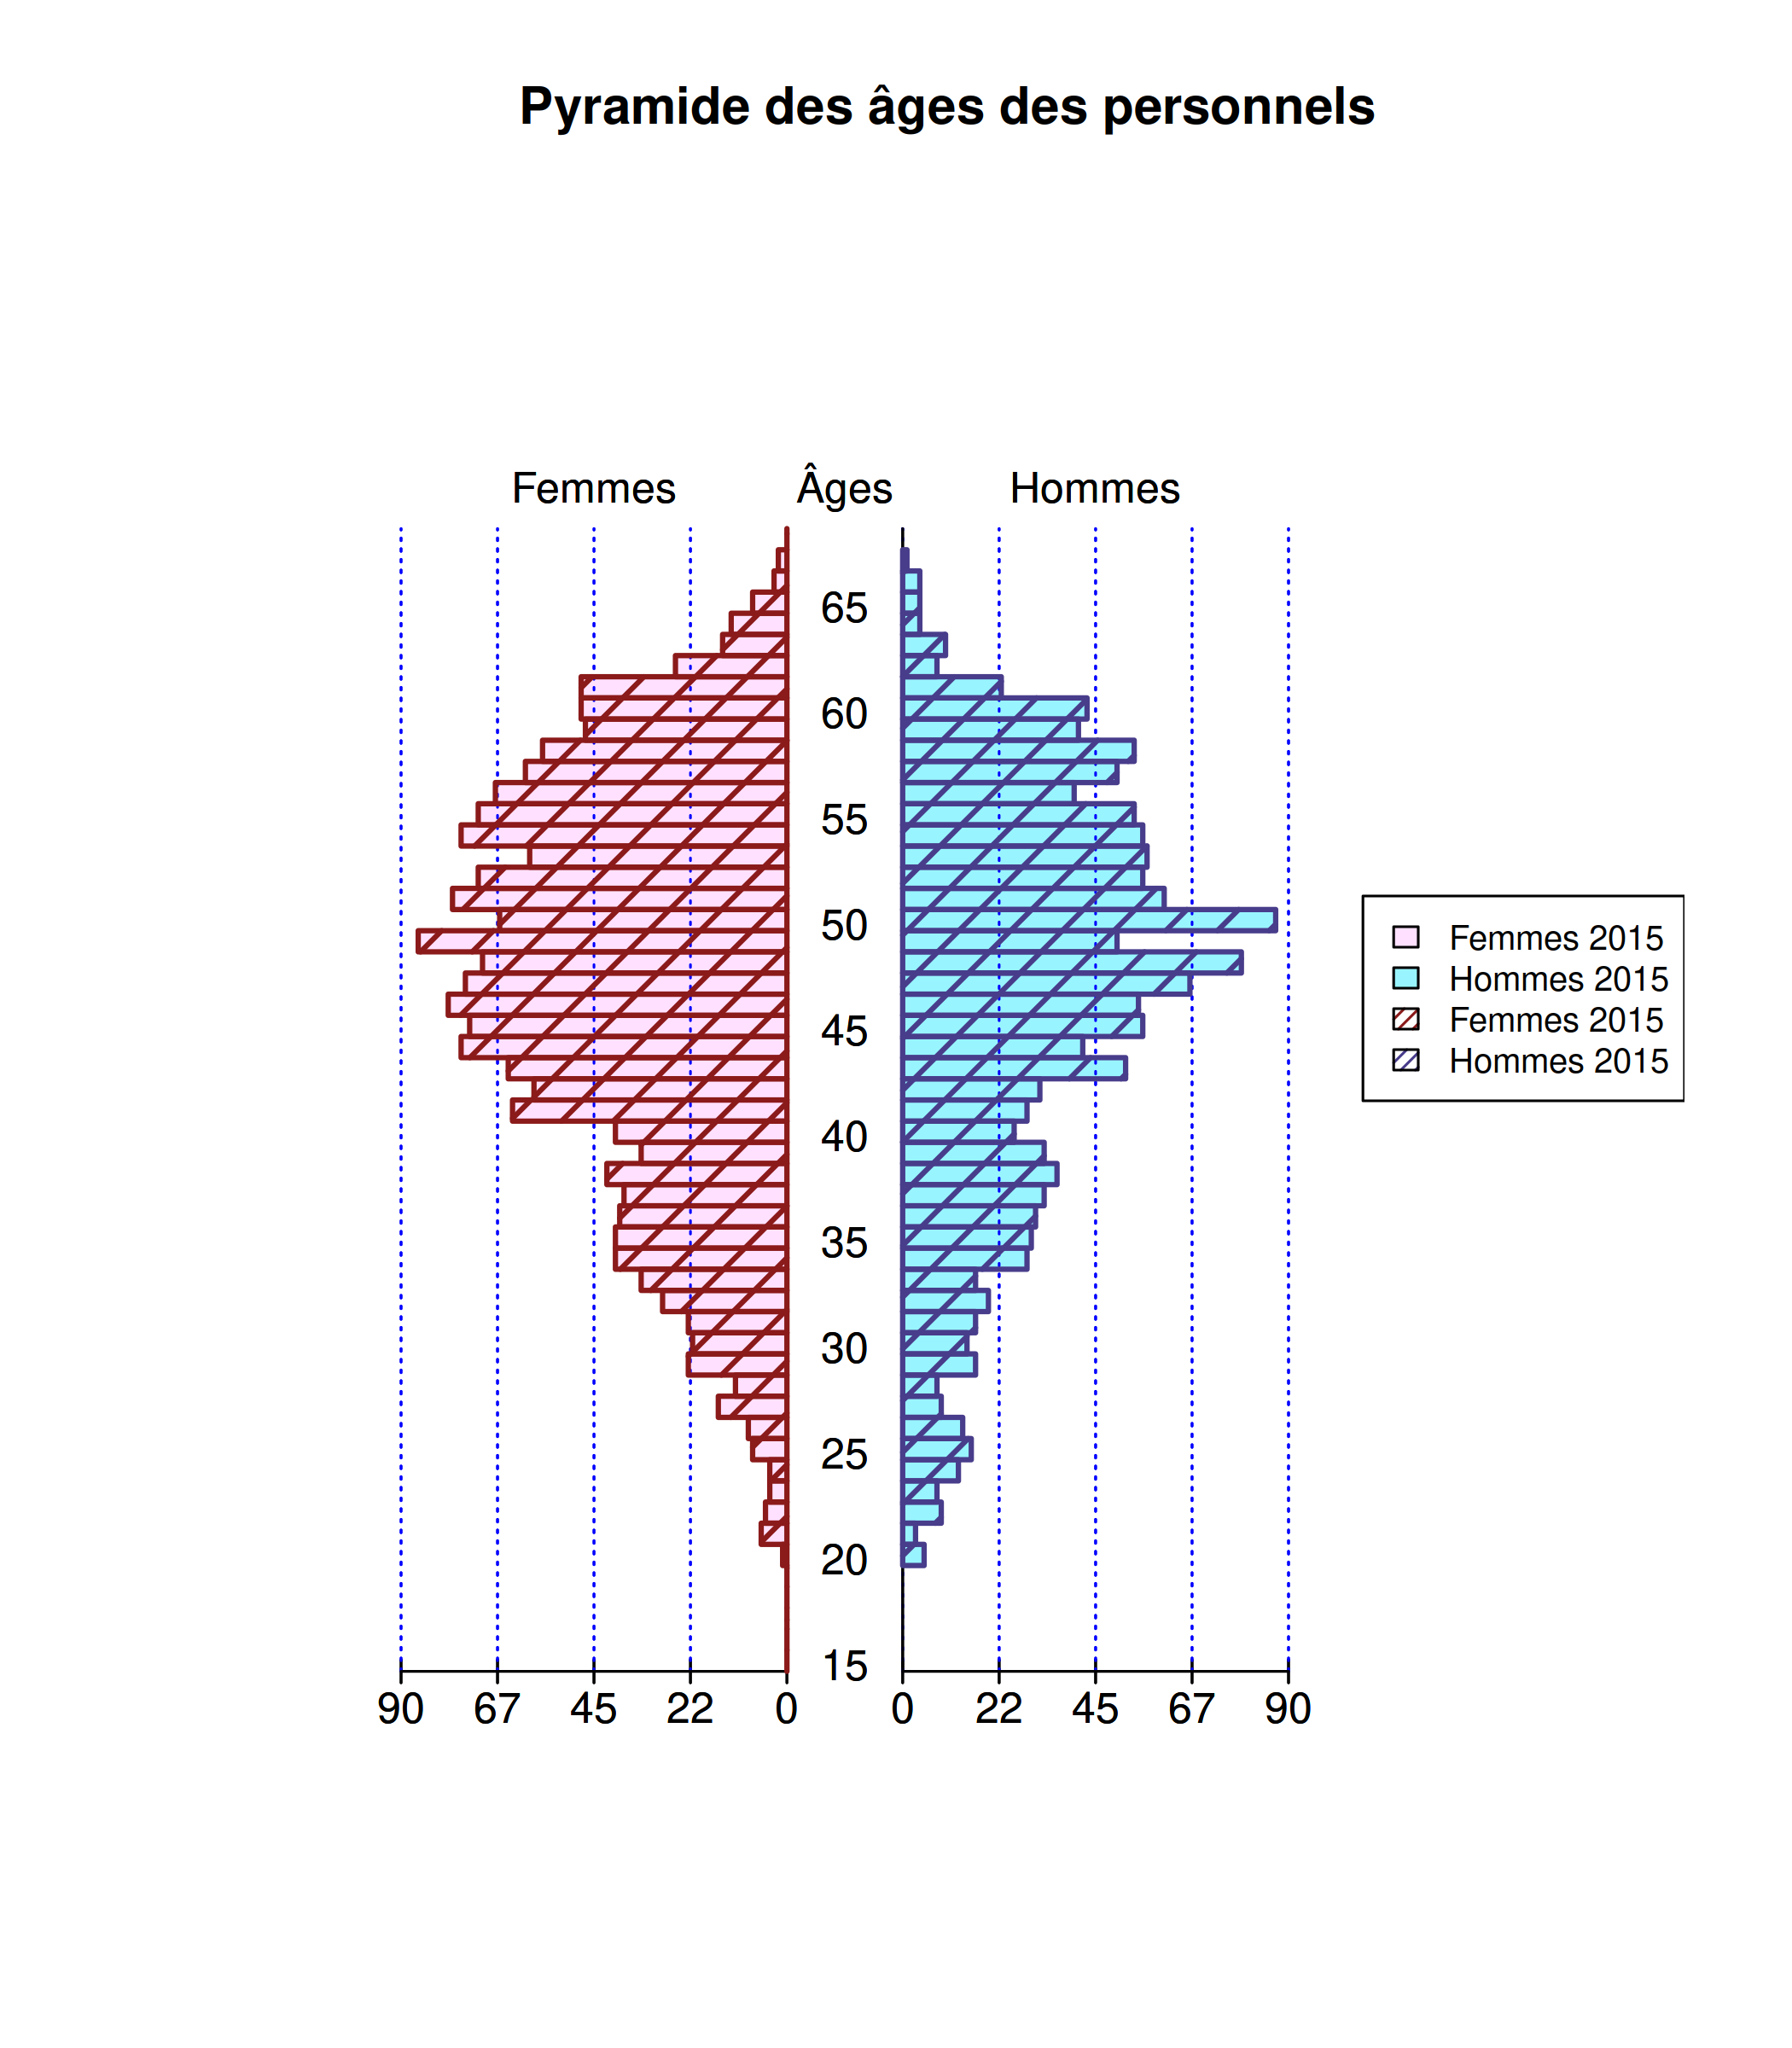
\includegraphics{altair_files/figure-latex/unnamed-chunk-11-1.png}
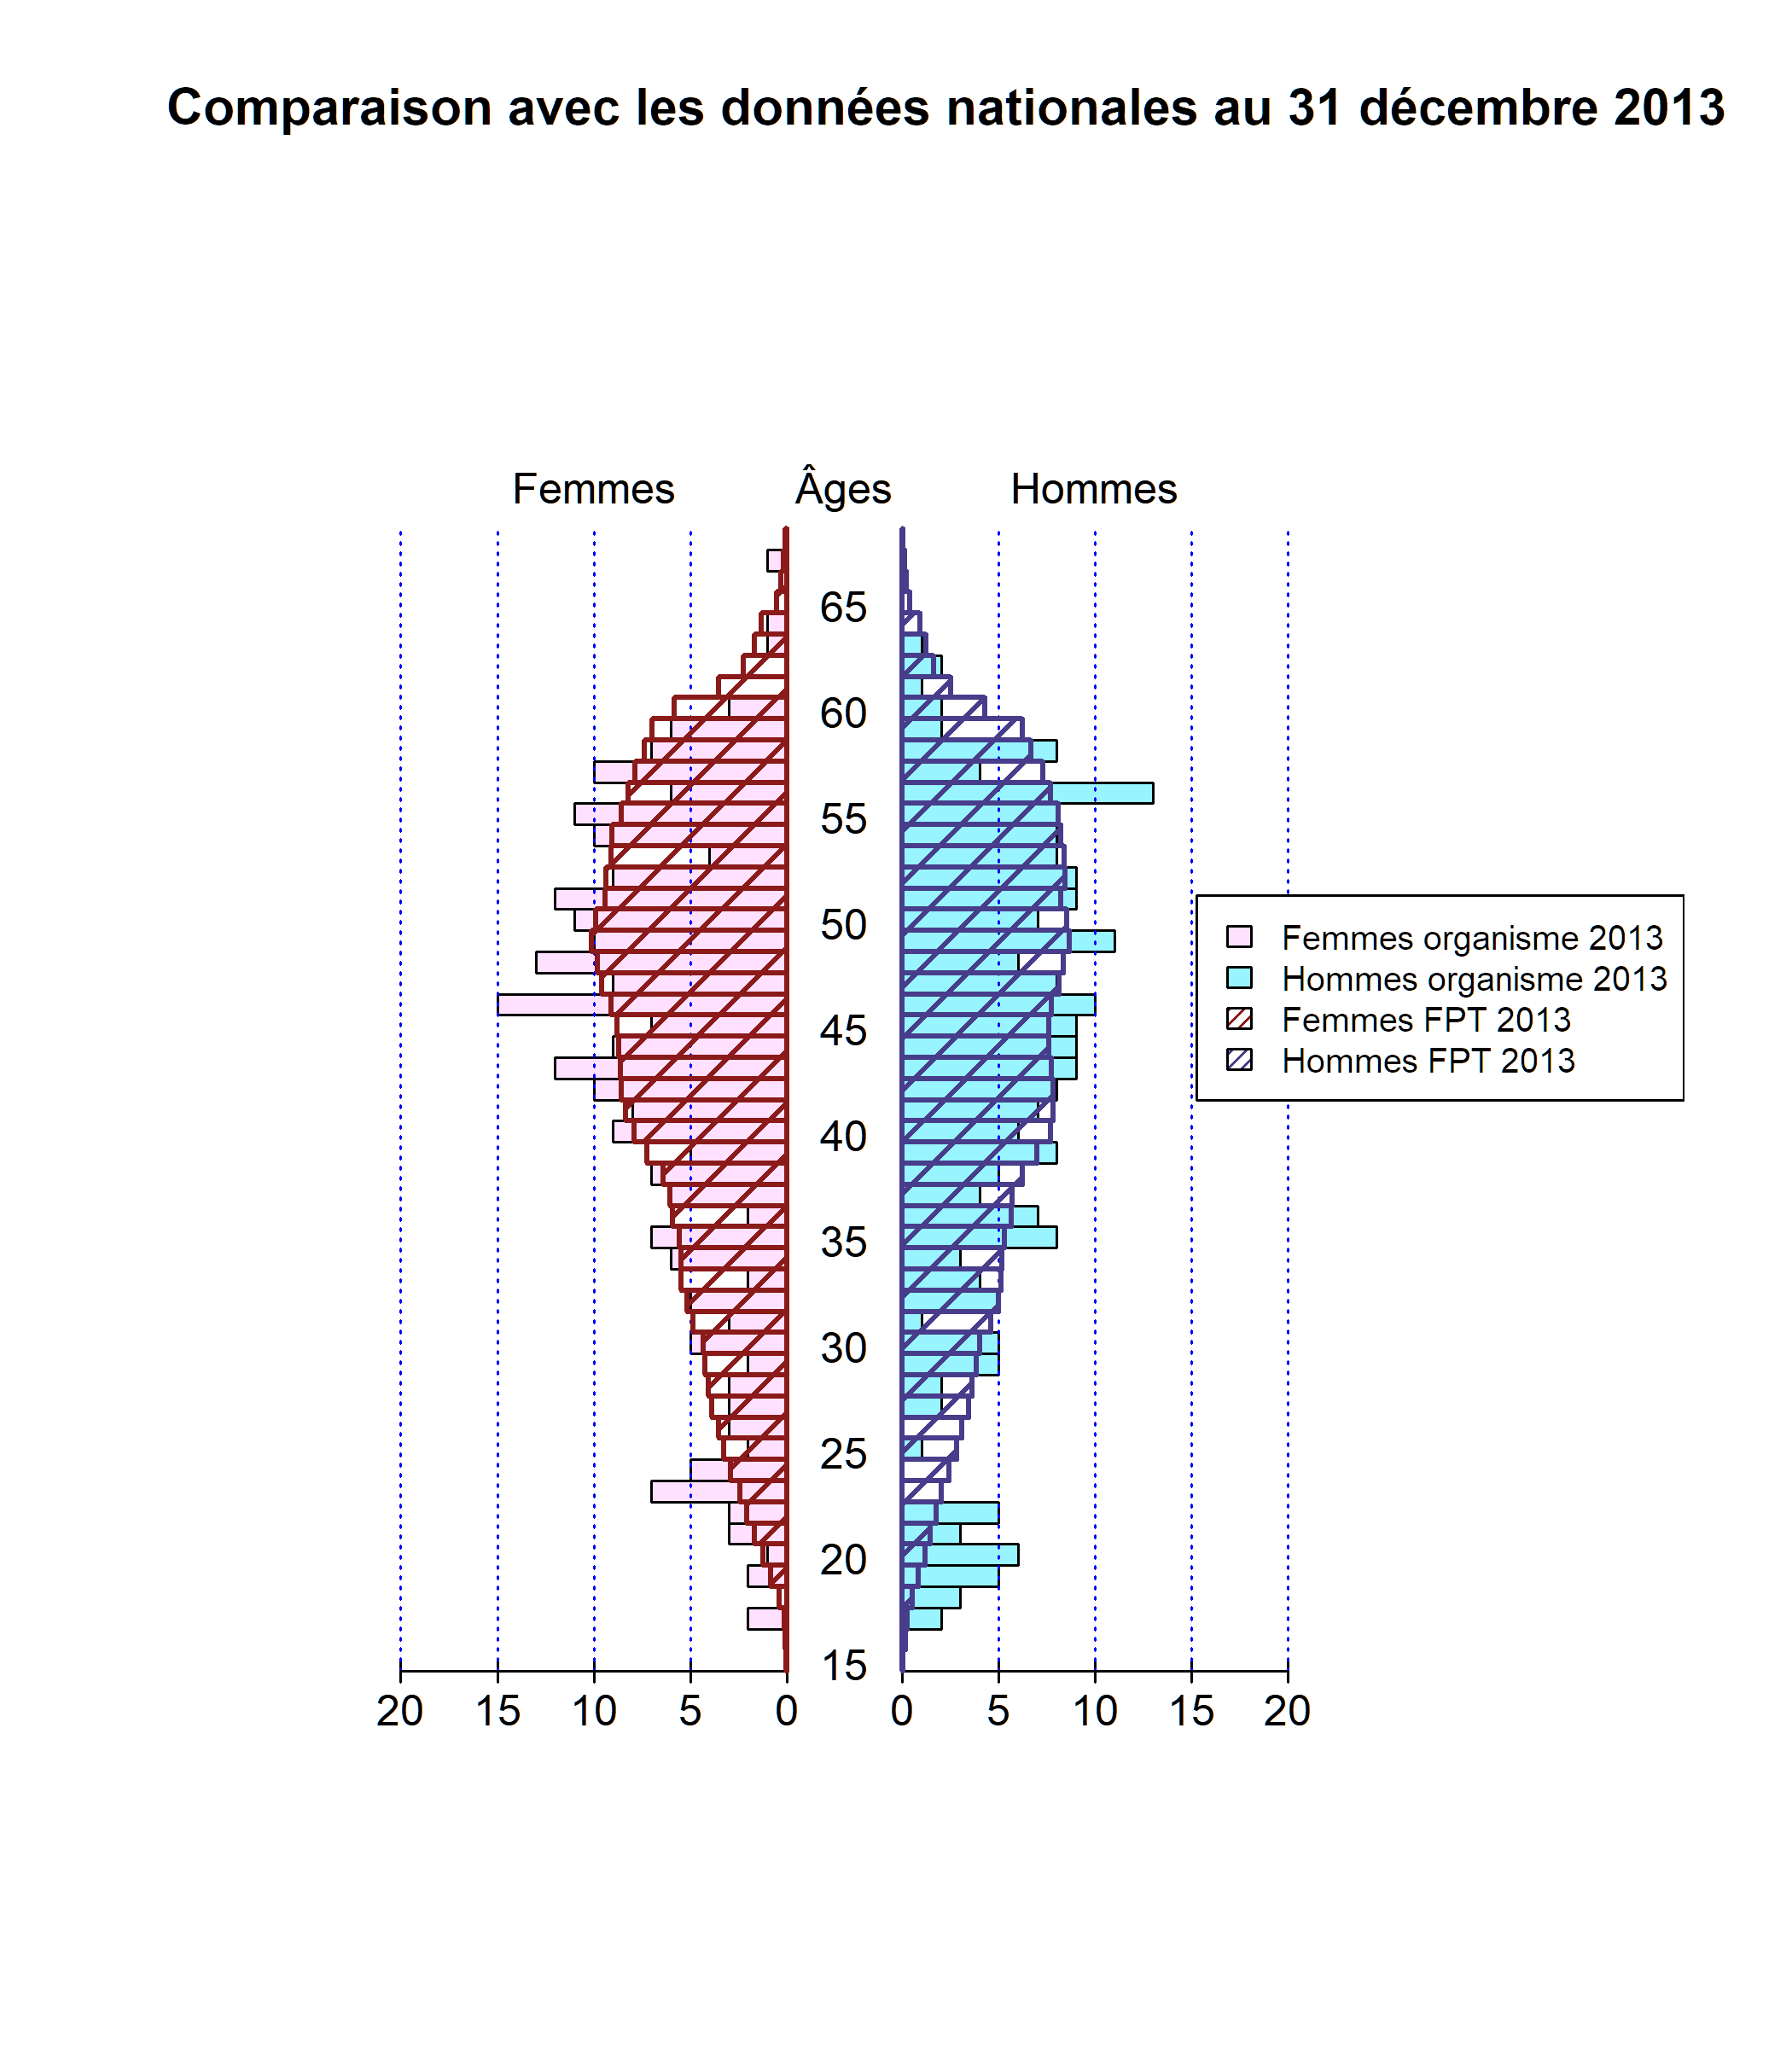
\includegraphics{altair_files/figure-latex/unnamed-chunk-11-2.png} Pour
obtenir les effectifs nationaux, multiplier les abscisses des hommes par
2 949 et les abscisses des femmes par 4 112\newpage
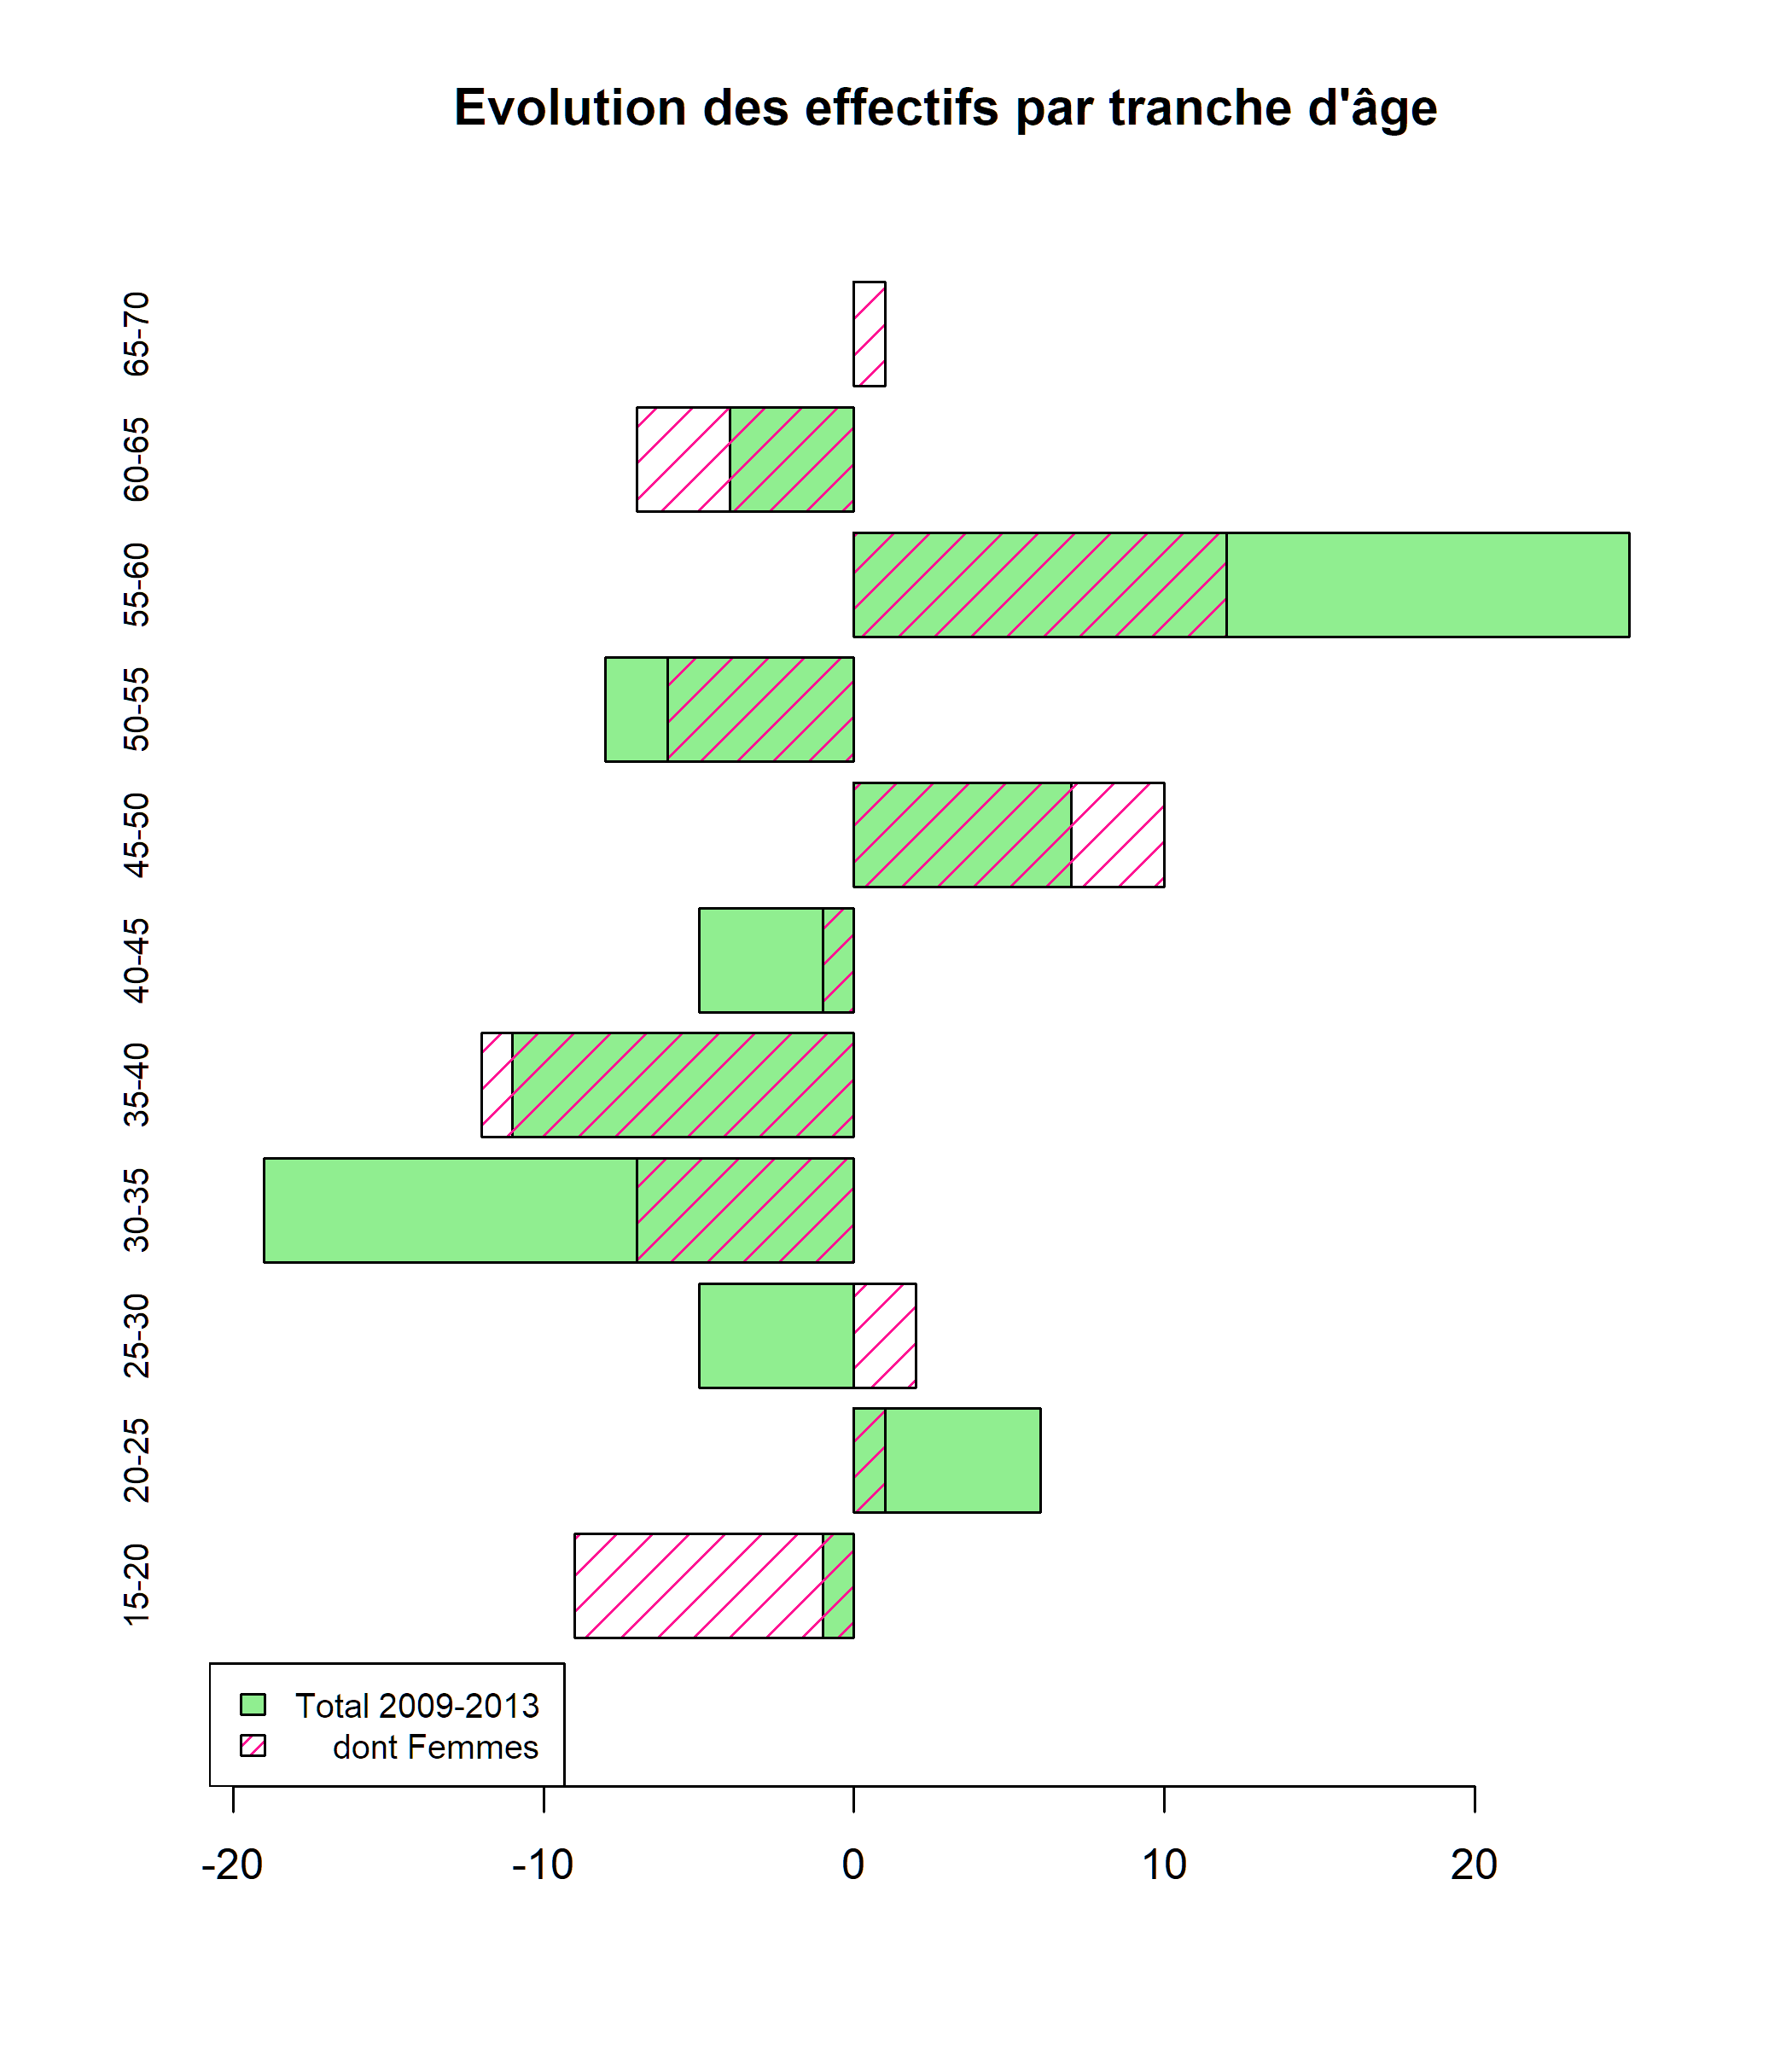
\includegraphics{altair_files/figure-latex/unnamed-chunk-11-3.png}

\href{Docs/Notices/fiche_3.odt}{
\includegraphics{icones/Notice.png}}

\newpage

~\emph{Tableau 1.2.1}

\begin{longtable}[]{@{}ccccc@{}}
\toprule
\begin{minipage}[b]{0.12\columnwidth}\centering
Statistique\strut
\end{minipage} & \begin{minipage}[b]{0.29\columnwidth}\centering
Âge des personnels au 31/12/2009\strut
\end{minipage} & \begin{minipage}[b]{0.08\columnwidth}\centering
Effectif\strut
\end{minipage} & \begin{minipage}[b]{0.29\columnwidth}\centering
Âge des personnels au 31/12/2013\strut
\end{minipage} & \begin{minipage}[b]{0.08\columnwidth}\centering
Effectif\strut
\end{minipage}\tabularnewline
\midrule
\endhead
\begin{minipage}[t]{0.12\columnwidth}\centering
Minimum\strut
\end{minipage} & \begin{minipage}[t]{0.29\columnwidth}\centering
16,0\strut
\end{minipage} & \begin{minipage}[t]{0.08\columnwidth}\centering
\strut
\end{minipage} & \begin{minipage}[t]{0.29\columnwidth}\centering
17,0\strut
\end{minipage} & \begin{minipage}[t]{0.08\columnwidth}\centering
\strut
\end{minipage}\tabularnewline
\begin{minipage}[t]{0.12\columnwidth}\centering
1er quartile\strut
\end{minipage} & \begin{minipage}[t]{0.29\columnwidth}\centering
35,0\strut
\end{minipage} & \begin{minipage}[t]{0.08\columnwidth}\centering
\strut
\end{minipage} & \begin{minipage}[t]{0.29\columnwidth}\centering
36,0\strut
\end{minipage} & \begin{minipage}[t]{0.08\columnwidth}\centering
\strut
\end{minipage}\tabularnewline
\begin{minipage}[t]{0.12\columnwidth}\centering
Médiane\strut
\end{minipage} & \begin{minipage}[t]{0.29\columnwidth}\centering
43,0\strut
\end{minipage} & \begin{minipage}[t]{0.08\columnwidth}\centering
\strut
\end{minipage} & \begin{minipage}[t]{0.29\columnwidth}\centering
45,0\strut
\end{minipage} & \begin{minipage}[t]{0.08\columnwidth}\centering
\strut
\end{minipage}\tabularnewline
\begin{minipage}[t]{0.12\columnwidth}\centering
Moyenne\strut
\end{minipage} & \begin{minipage}[t]{0.29\columnwidth}\centering
42,4\strut
\end{minipage} & \begin{minipage}[t]{0.08\columnwidth}\centering
542\strut
\end{minipage} & \begin{minipage}[t]{0.29\columnwidth}\centering
43,4\strut
\end{minipage} & \begin{minipage}[t]{0.08\columnwidth}\centering
528\strut
\end{minipage}\tabularnewline
\begin{minipage}[t]{0.12\columnwidth}\centering
3ème quartile\strut
\end{minipage} & \begin{minipage}[t]{0.29\columnwidth}\centering
51,0\strut
\end{minipage} & \begin{minipage}[t]{0.08\columnwidth}\centering
\strut
\end{minipage} & \begin{minipage}[t]{0.29\columnwidth}\centering
52,0\strut
\end{minipage} & \begin{minipage}[t]{0.08\columnwidth}\centering
\strut
\end{minipage}\tabularnewline
\begin{minipage}[t]{0.12\columnwidth}\centering
Maximum\strut
\end{minipage} & \begin{minipage}[t]{0.29\columnwidth}\centering
66,0\strut
\end{minipage} & \begin{minipage}[t]{0.08\columnwidth}\centering
\strut
\end{minipage} & \begin{minipage}[t]{0.29\columnwidth}\centering
70,0\strut
\end{minipage} & \begin{minipage}[t]{0.08\columnwidth}\centering
\strut
\end{minipage}\tabularnewline
\bottomrule
\end{longtable}

\href{Docs/Notices/fiche_1.odt}{
\includegraphics{icones/Notice.png}}

\href{Bases/Effectifs/Pyramide-des-ages-des-personnels_2009.csv}{Lien
vers la base des âges - début de periode}

\href{Bases/Effectifs/Pyramide-des-ages-des-personnels_2013.csv}{Lien
vers la base des âges - fin de periode}

\hypertarget{pyramide-des-ages-des-fonctionnaires}{%
\subsection{1.3 Pyramide des âges des fonctionnaires
~}\label{pyramide-des-ages-des-fonctionnaires}}

\href{Docs/Notices/fiche_2.odt}{
\includegraphics{icones/Notice.png}}

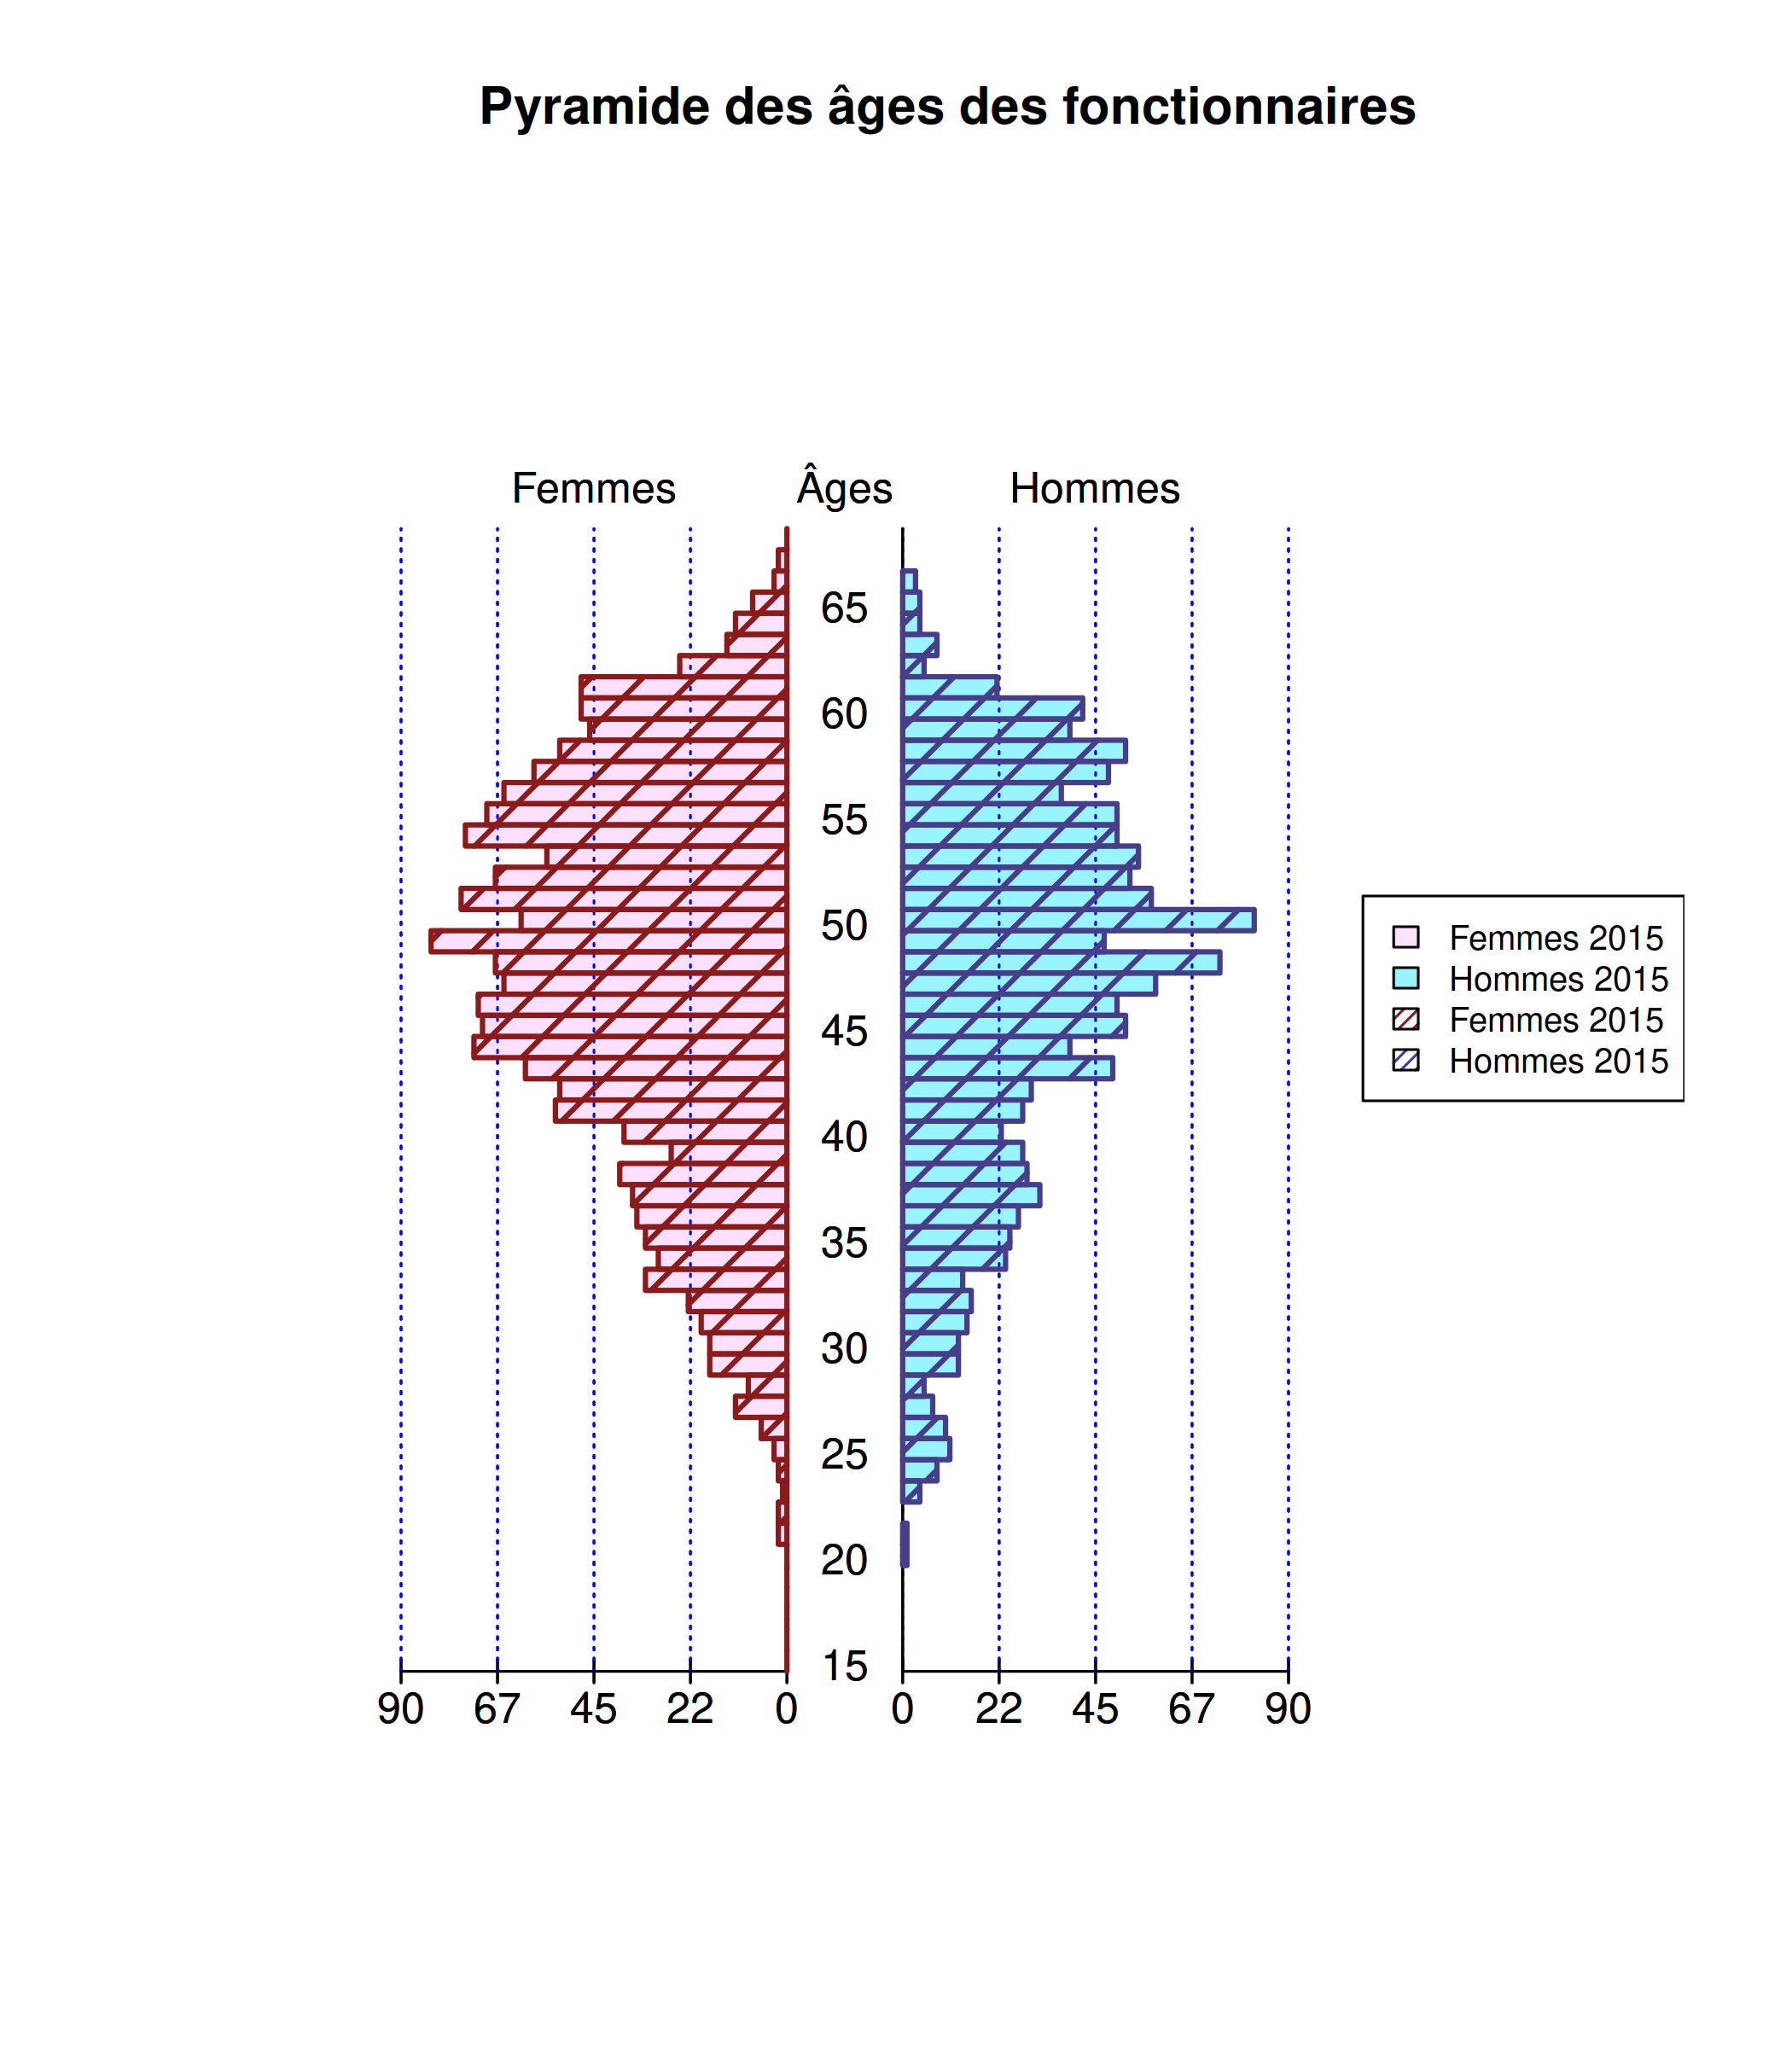
\includegraphics{altair_files/figure-latex/unnamed-chunk-17-1.png}
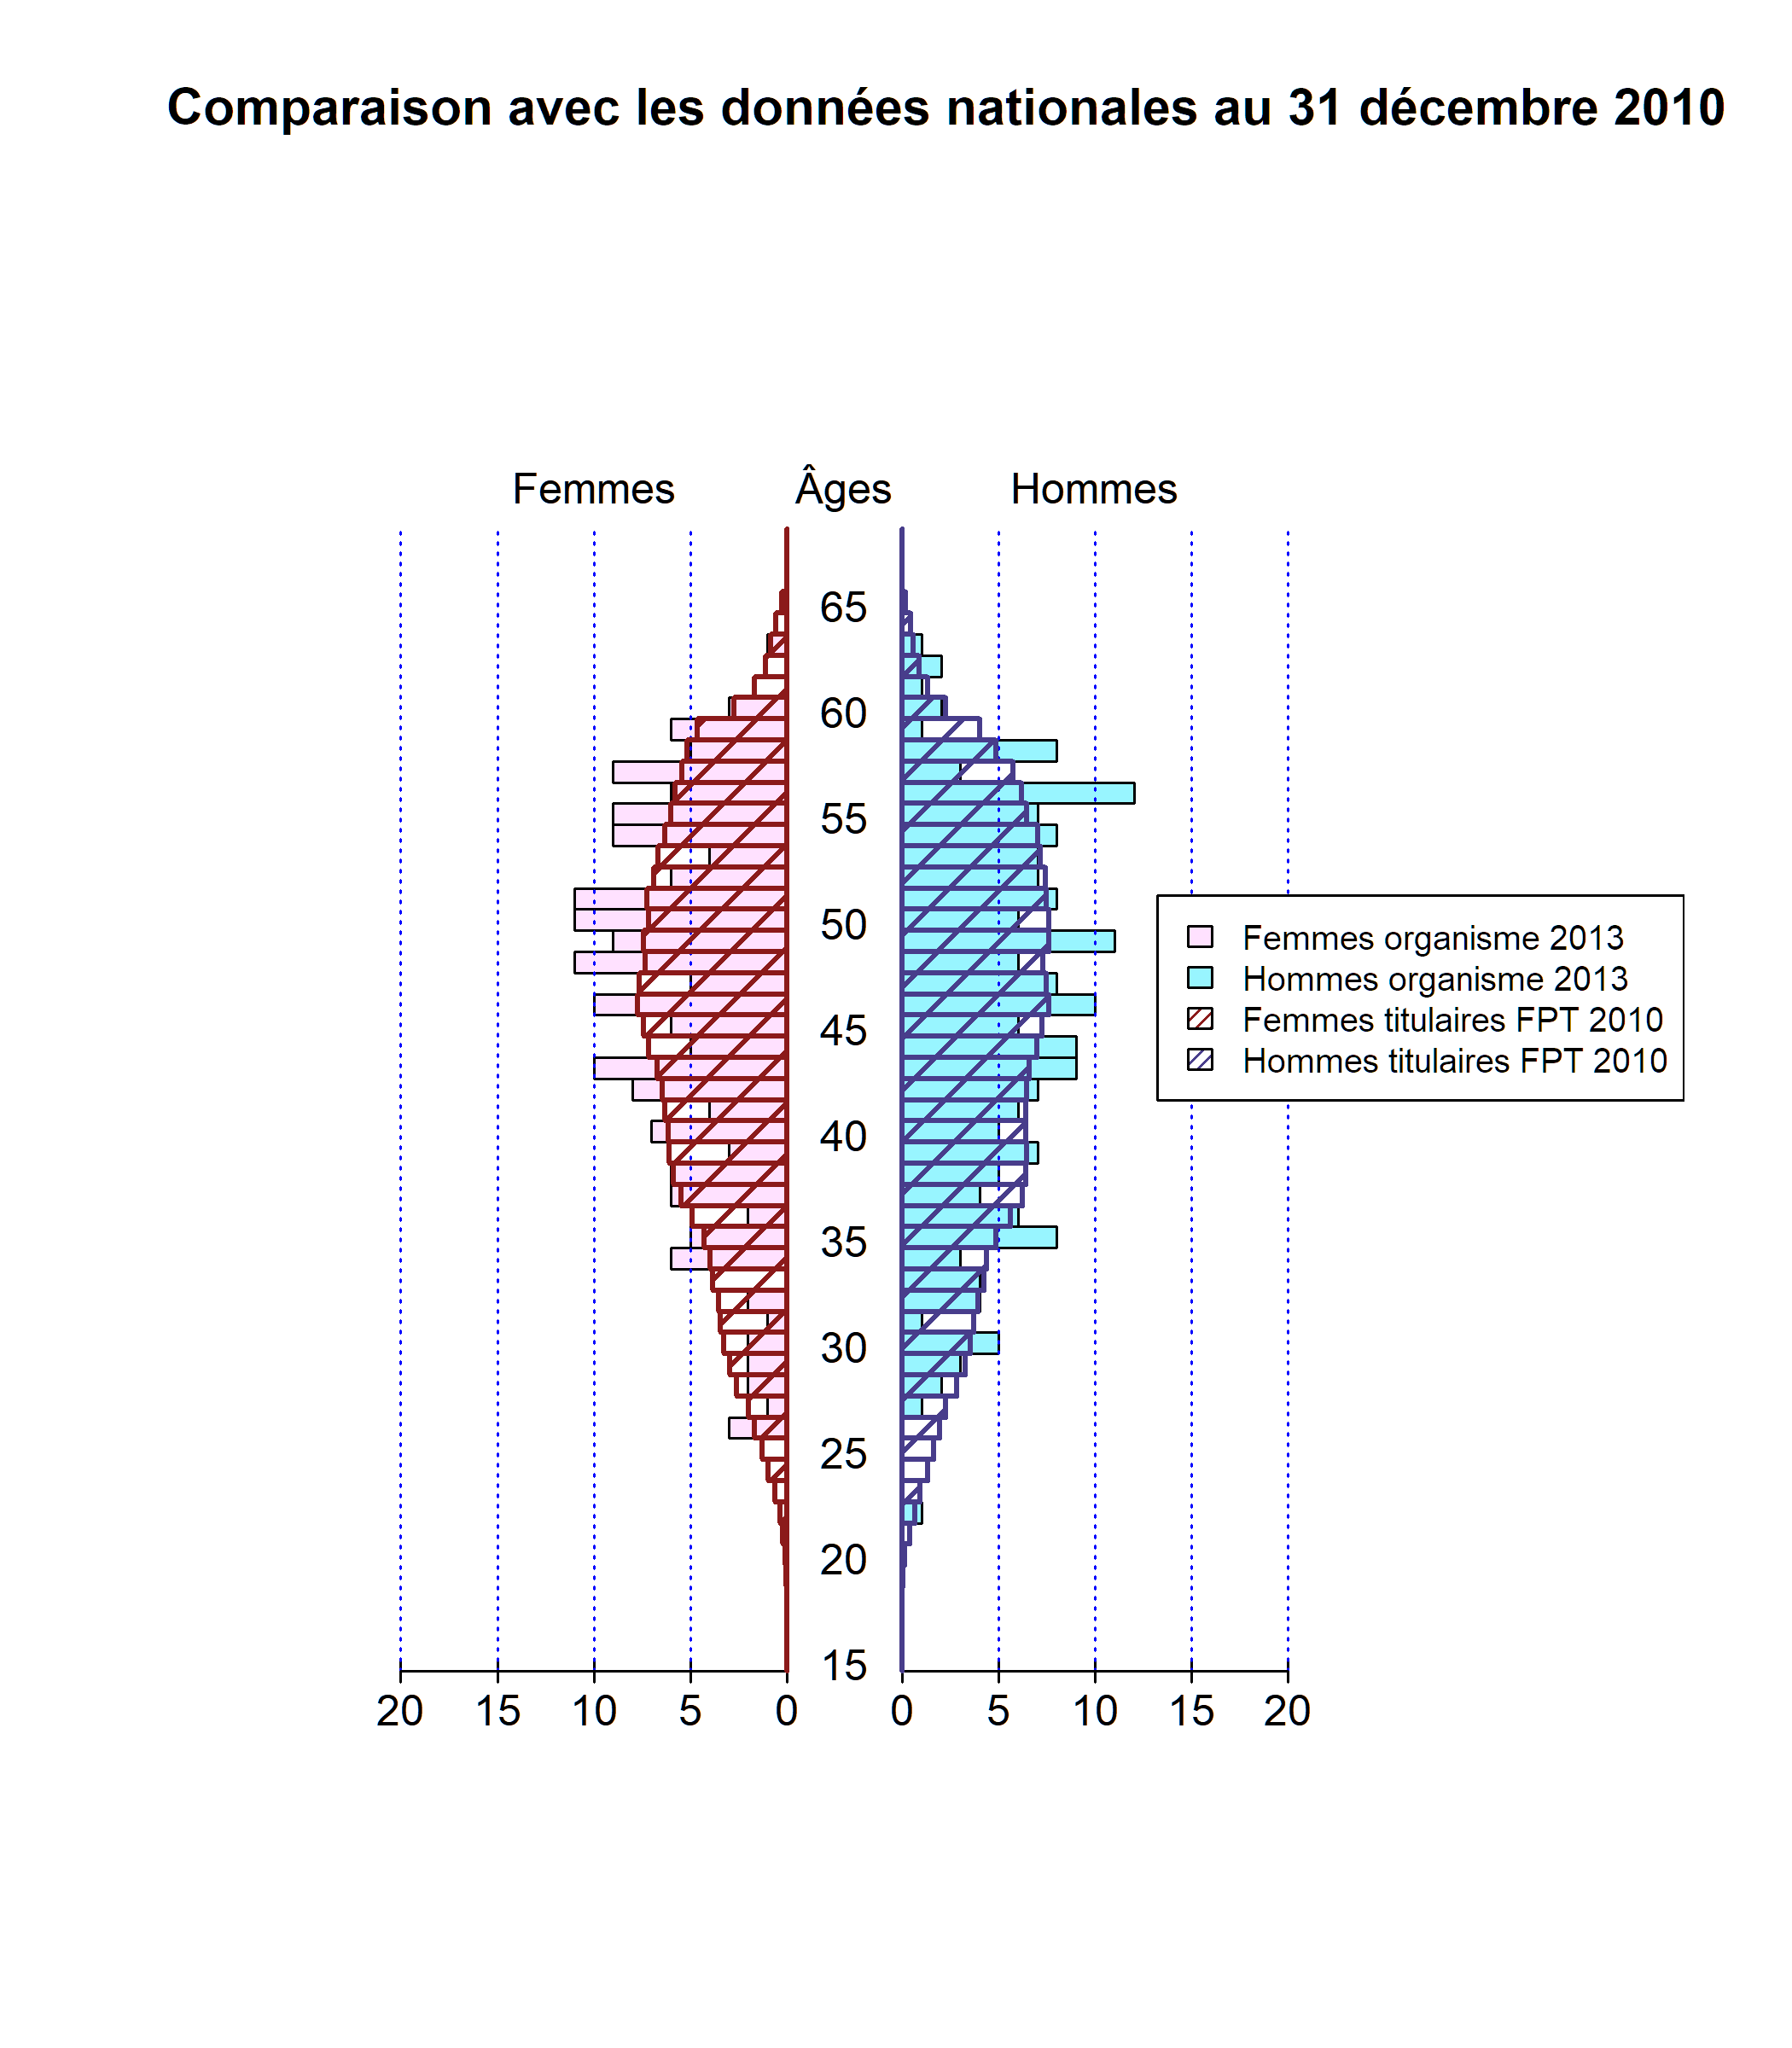
\includegraphics{altair_files/figure-latex/unnamed-chunk-17-2.png} Pour
obtenir les effectifs nationaux, multiplier les abscisses des hommes par
2 314 et les abscisses des femmes par 1 214\newpage
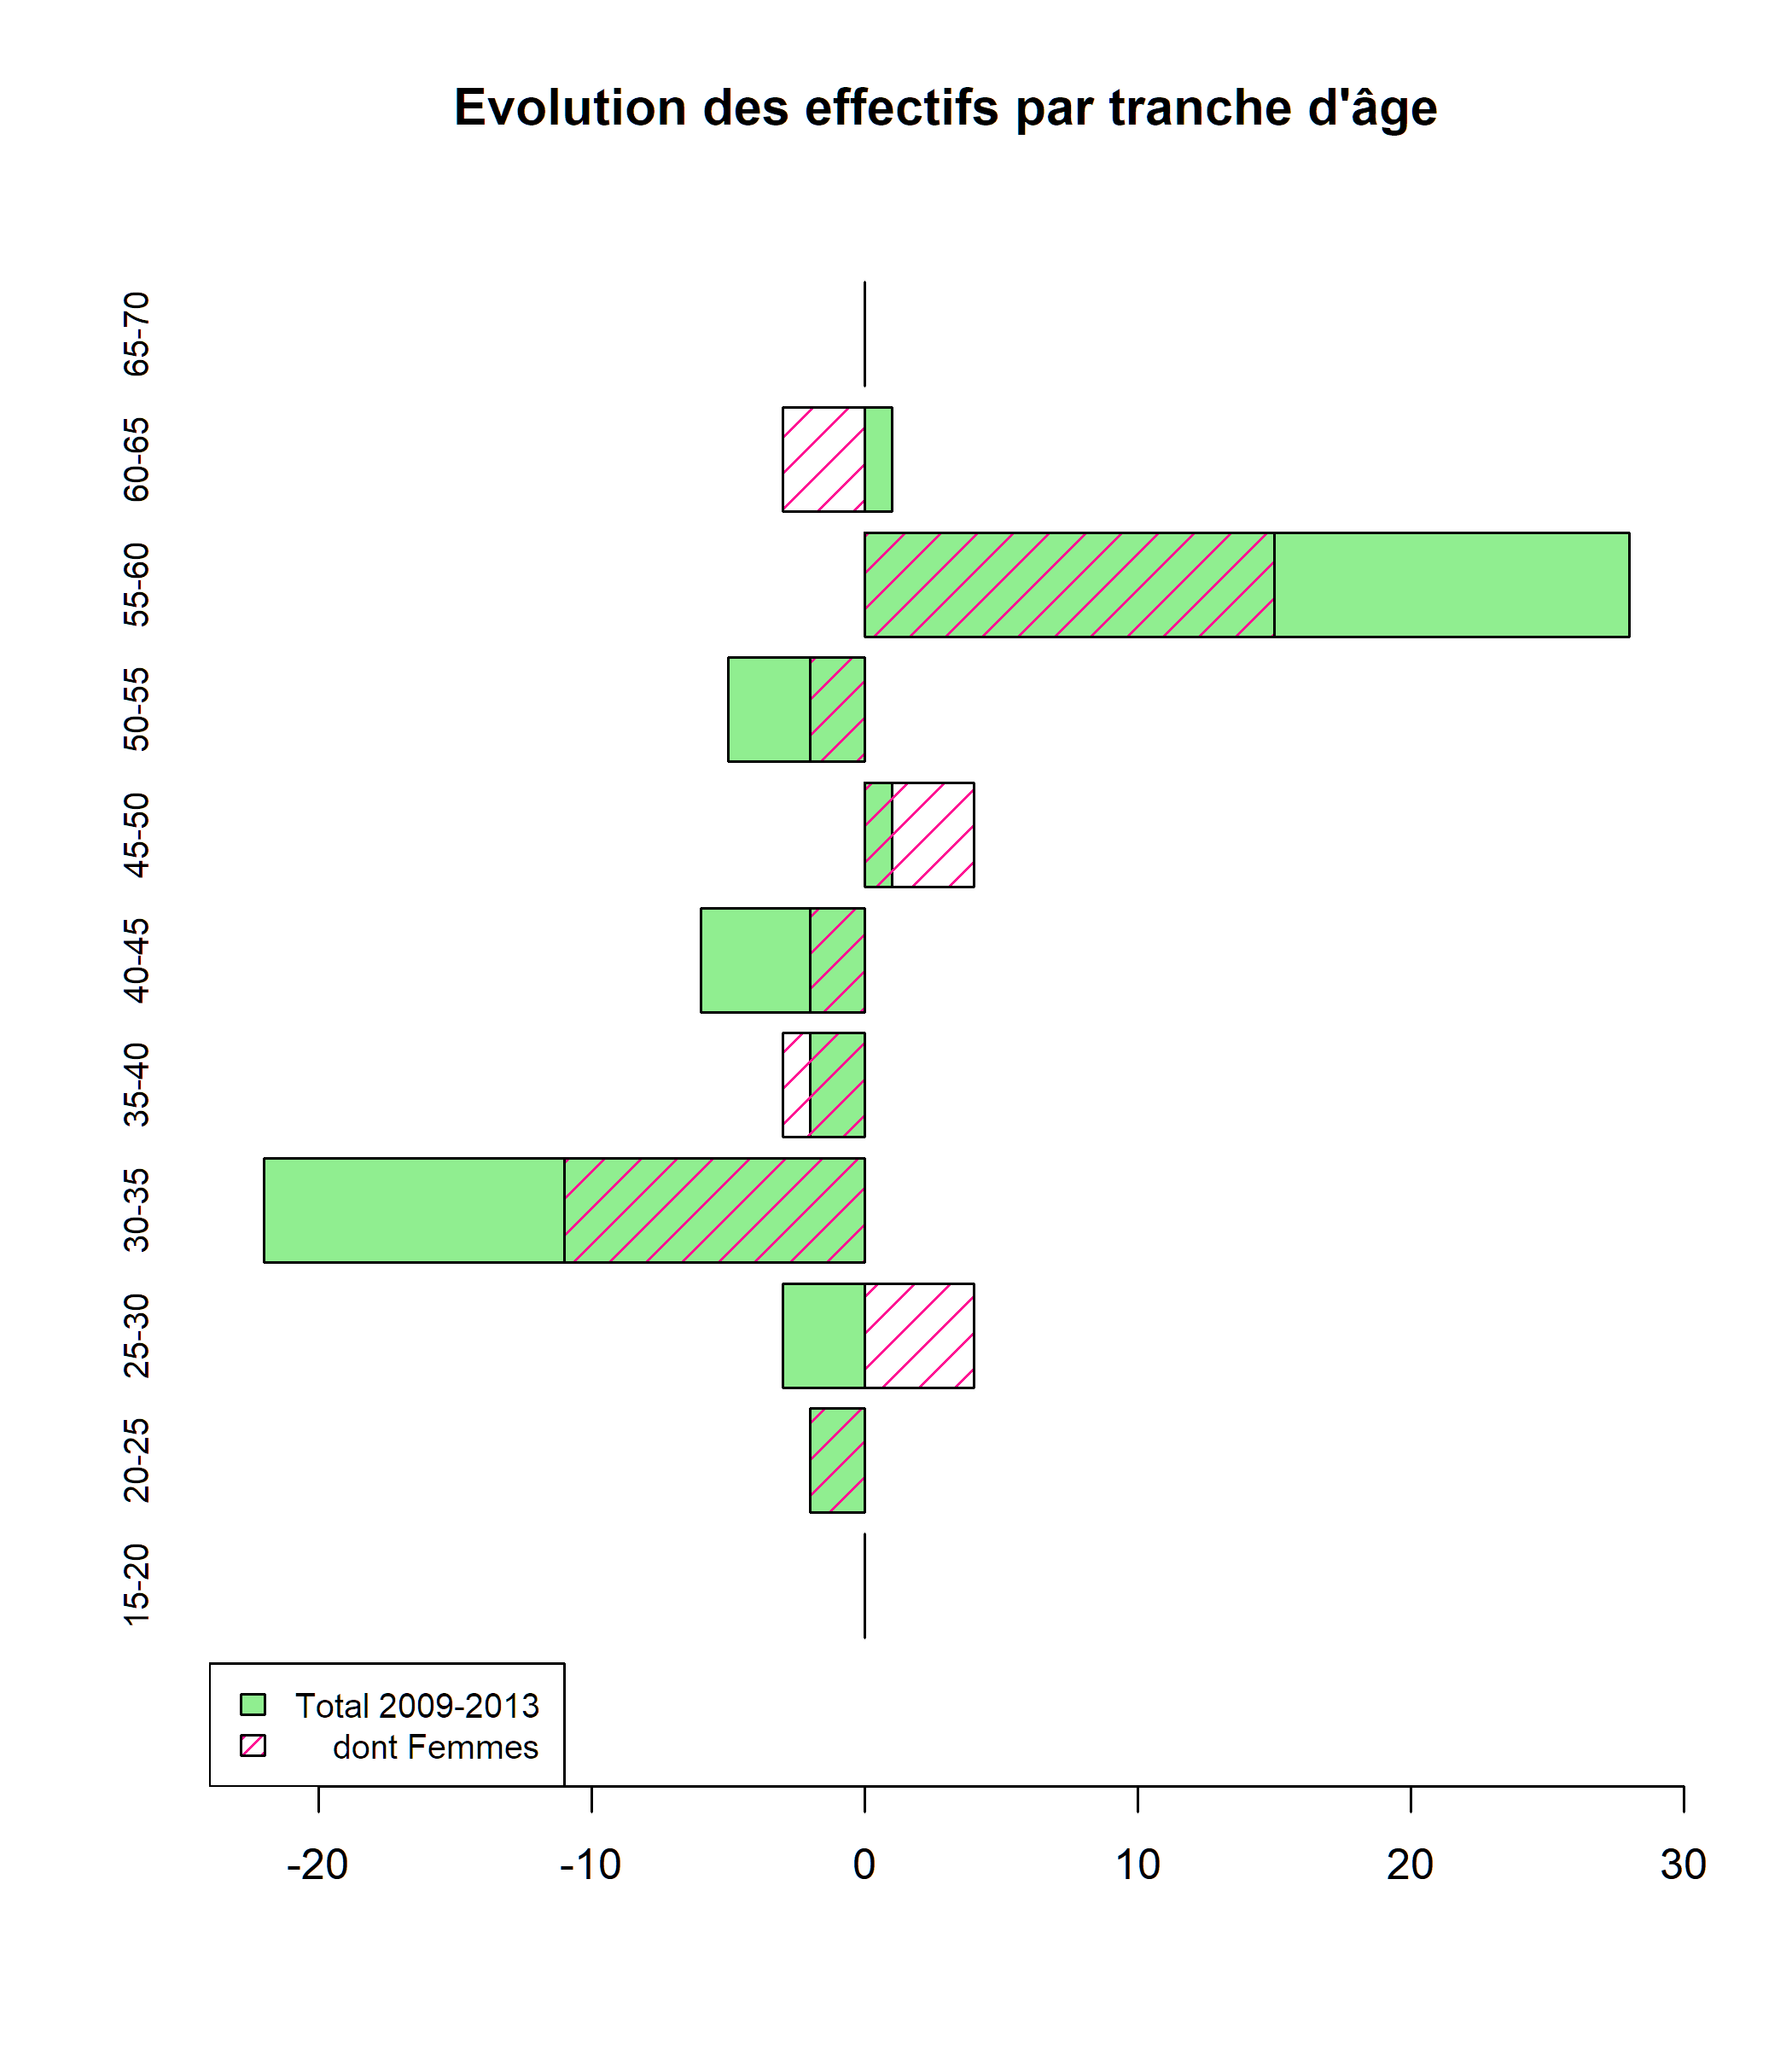
\includegraphics{altair_files/figure-latex/unnamed-chunk-17-3.png}

\href{Docs/Notices/fiche_3.odt}{
\includegraphics{icones/Notice.png}}

\newpage

~\emph{Tableau 1.3.1}

\begin{longtable}[]{@{}ccccc@{}}
\toprule
\begin{minipage}[b]{0.12\columnwidth}\centering
Statistique\strut
\end{minipage} & \begin{minipage}[b]{0.29\columnwidth}\centering
Âge des personnels au 31/12/2009\strut
\end{minipage} & \begin{minipage}[b]{0.08\columnwidth}\centering
Effectif\strut
\end{minipage} & \begin{minipage}[b]{0.29\columnwidth}\centering
Âge des personnels au 31/12/2013\strut
\end{minipage} & \begin{minipage}[b]{0.08\columnwidth}\centering
Effectif\strut
\end{minipage}\tabularnewline
\midrule
\endhead
\begin{minipage}[t]{0.12\columnwidth}\centering
Minimum\strut
\end{minipage} & \begin{minipage}[t]{0.29\columnwidth}\centering
24,0\strut
\end{minipage} & \begin{minipage}[t]{0.08\columnwidth}\centering
\strut
\end{minipage} & \begin{minipage}[t]{0.29\columnwidth}\centering
22,0\strut
\end{minipage} & \begin{minipage}[t]{0.08\columnwidth}\centering
\strut
\end{minipage}\tabularnewline
\begin{minipage}[t]{0.12\columnwidth}\centering
1er quartile\strut
\end{minipage} & \begin{minipage}[t]{0.29\columnwidth}\centering
38,0\strut
\end{minipage} & \begin{minipage}[t]{0.08\columnwidth}\centering
\strut
\end{minipage} & \begin{minipage}[t]{0.29\columnwidth}\centering
40,0\strut
\end{minipage} & \begin{minipage}[t]{0.08\columnwidth}\centering
\strut
\end{minipage}\tabularnewline
\begin{minipage}[t]{0.12\columnwidth}\centering
Médiane\strut
\end{minipage} & \begin{minipage}[t]{0.29\columnwidth}\centering
45,0\strut
\end{minipage} & \begin{minipage}[t]{0.08\columnwidth}\centering
\strut
\end{minipage} & \begin{minipage}[t]{0.29\columnwidth}\centering
47,0\strut
\end{minipage} & \begin{minipage}[t]{0.08\columnwidth}\centering
\strut
\end{minipage}\tabularnewline
\begin{minipage}[t]{0.12\columnwidth}\centering
Moyenne\strut
\end{minipage} & \begin{minipage}[t]{0.29\columnwidth}\centering
44,2\strut
\end{minipage} & \begin{minipage}[t]{0.08\columnwidth}\centering
410\strut
\end{minipage} & \begin{minipage}[t]{0.29\columnwidth}\centering
46,0\strut
\end{minipage} & \begin{minipage}[t]{0.08\columnwidth}\centering
400\strut
\end{minipage}\tabularnewline
\begin{minipage}[t]{0.12\columnwidth}\centering
3ème quartile\strut
\end{minipage} & \begin{minipage}[t]{0.29\columnwidth}\centering
51,0\strut
\end{minipage} & \begin{minipage}[t]{0.08\columnwidth}\centering
\strut
\end{minipage} & \begin{minipage}[t]{0.29\columnwidth}\centering
53,0\strut
\end{minipage} & \begin{minipage}[t]{0.08\columnwidth}\centering
\strut
\end{minipage}\tabularnewline
\begin{minipage}[t]{0.12\columnwidth}\centering
Maximum\strut
\end{minipage} & \begin{minipage}[t]{0.29\columnwidth}\centering
62,0\strut
\end{minipage} & \begin{minipage}[t]{0.08\columnwidth}\centering
\strut
\end{minipage} & \begin{minipage}[t]{0.29\columnwidth}\centering
63,0\strut
\end{minipage} & \begin{minipage}[t]{0.08\columnwidth}\centering
\strut
\end{minipage}\tabularnewline
\bottomrule
\end{longtable}

\href{Bases/Effectifs/Pyramide-des-ages-des-fonctionnaires_2009.csv}{Lien
vers la base des âges - début de periode}

\href{Bases/Effectifs/Pyramide-des-ages-des-fonctionnaires_2013.csv}{Lien
vers la base des âges - fin de periode}

\href{Docs/Notices/fiche_1.odt}{
\includegraphics{icones/Notice.png}}

\hypertarget{pyramide-des-ages-personnels-non-titulaires}{%
\subsection{1.4 Pyramide des âges, personnels non titulaires
~}\label{pyramide-des-ages-personnels-non-titulaires}}

\href{Docs/Notices/fiche_2.odt}{
\includegraphics{icones/Notice.png}}

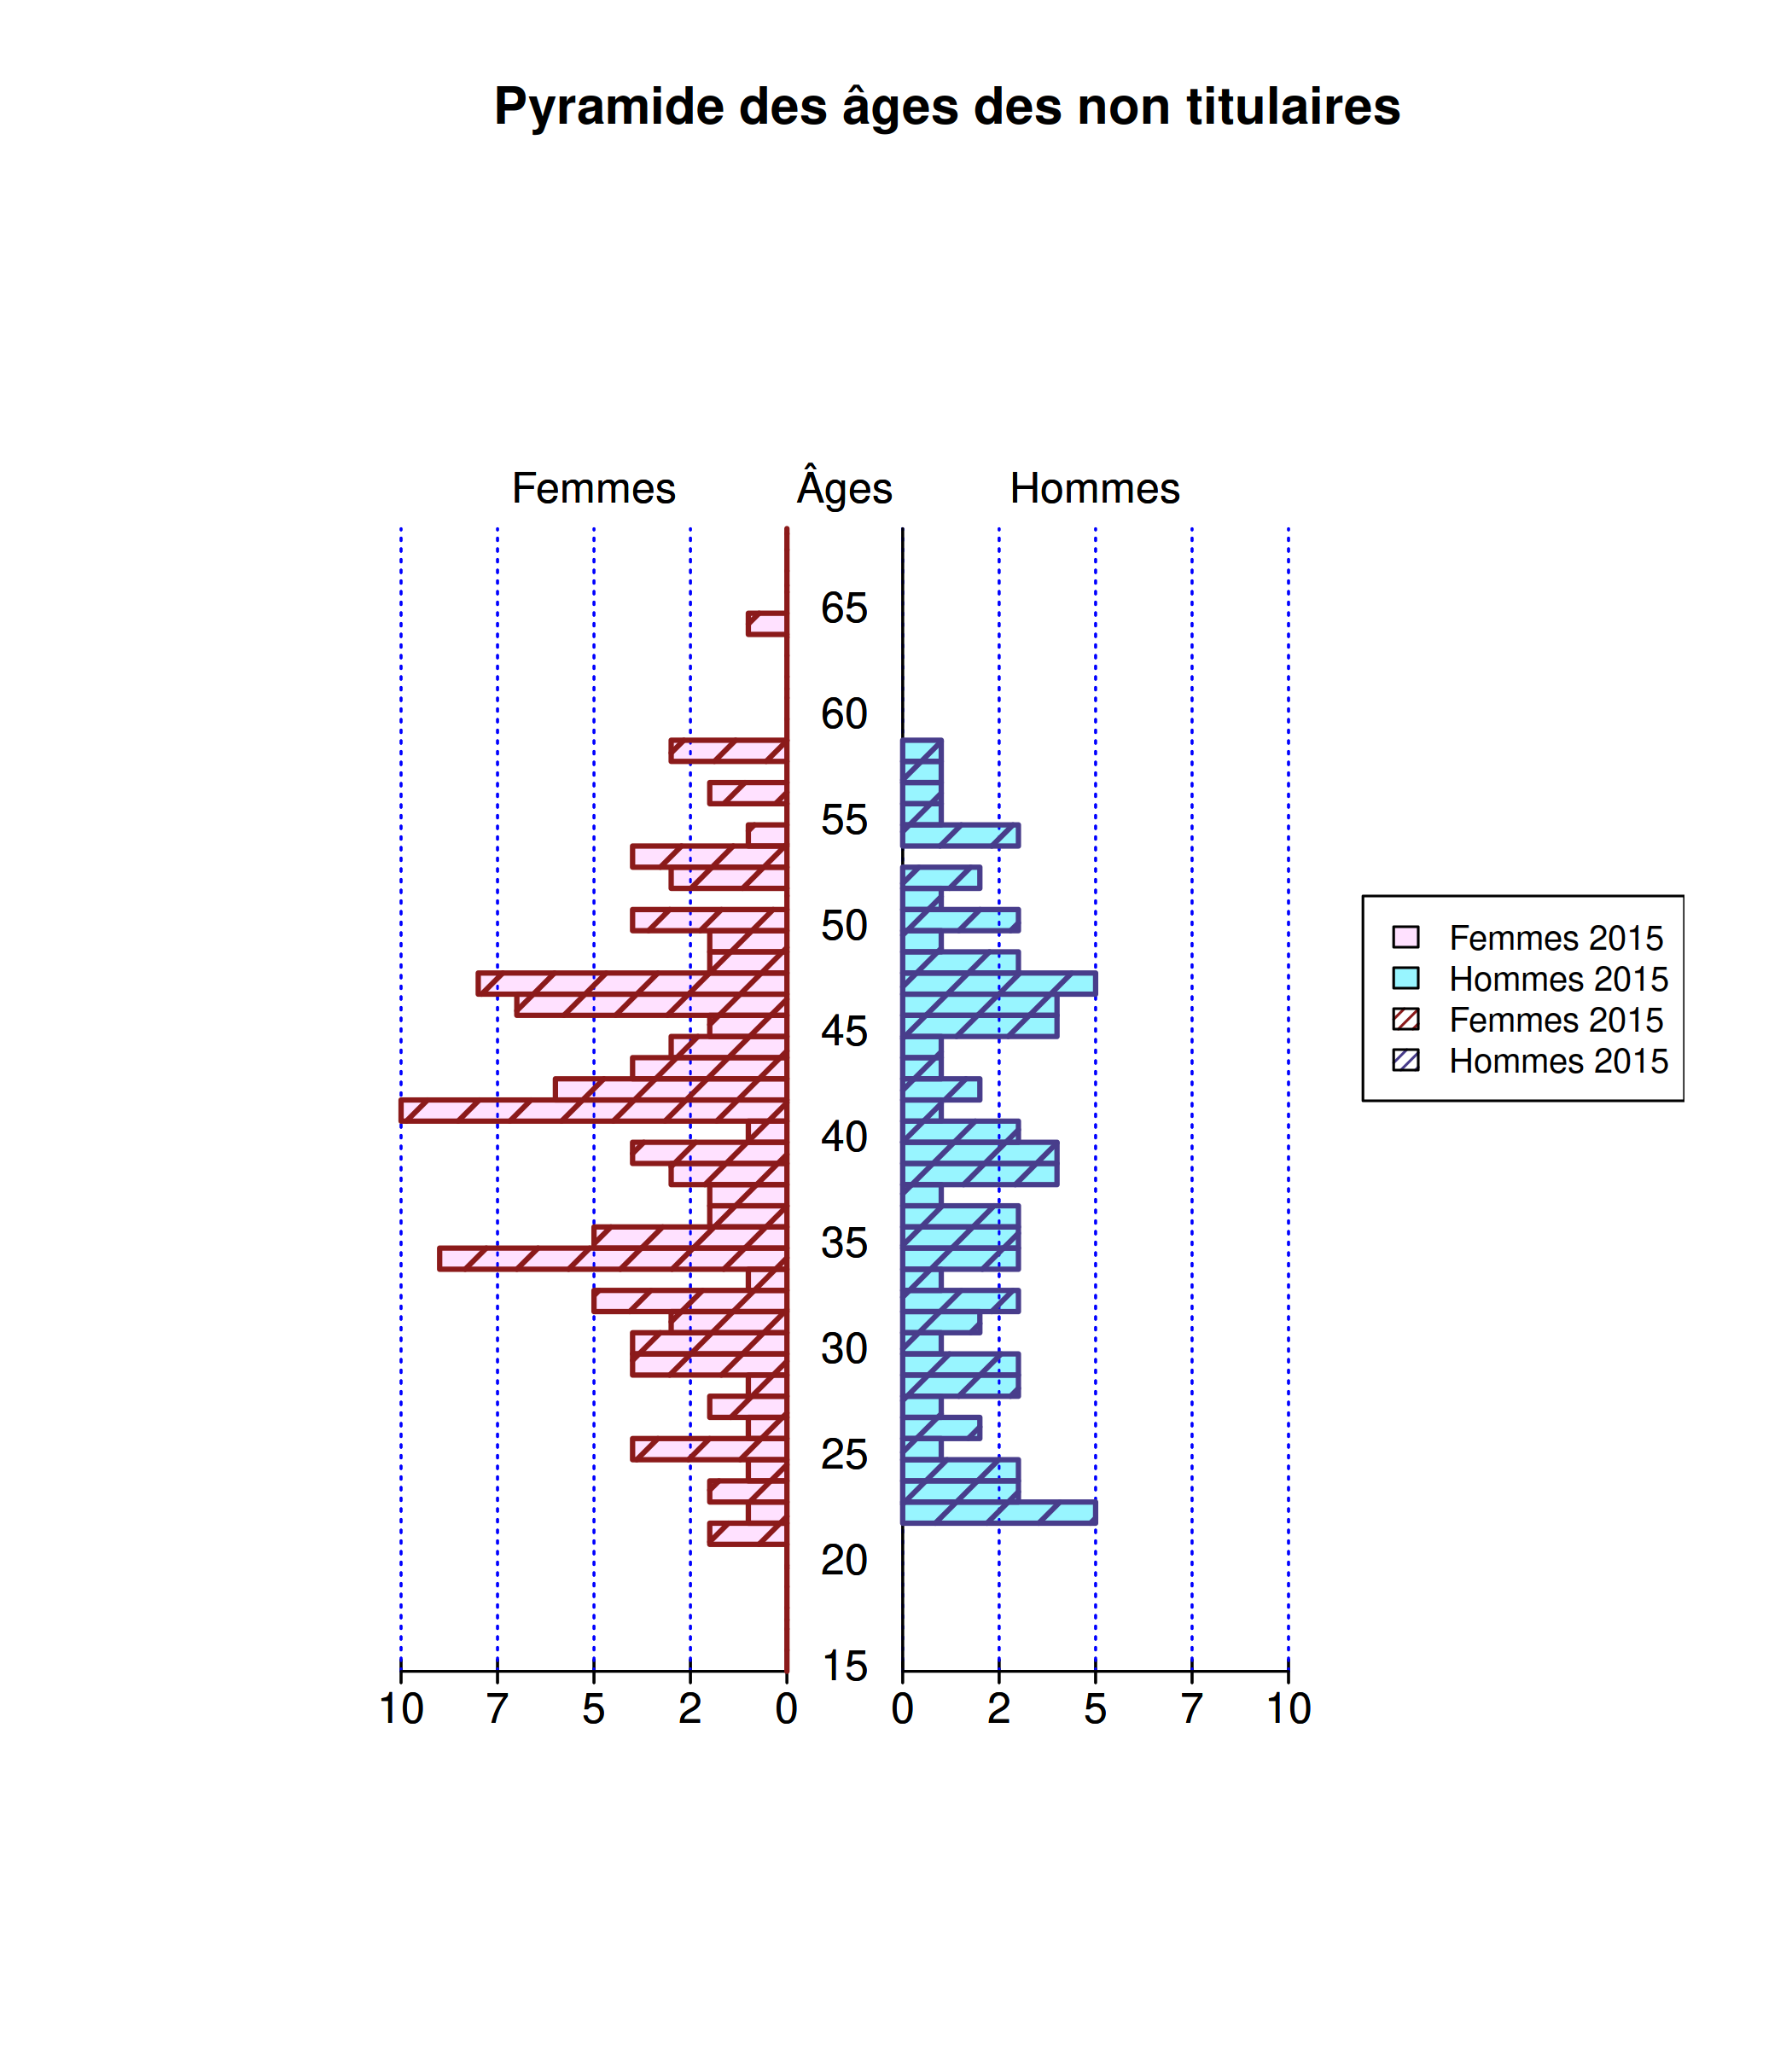
\includegraphics{altair_files/figure-latex/unnamed-chunk-23-1.png}
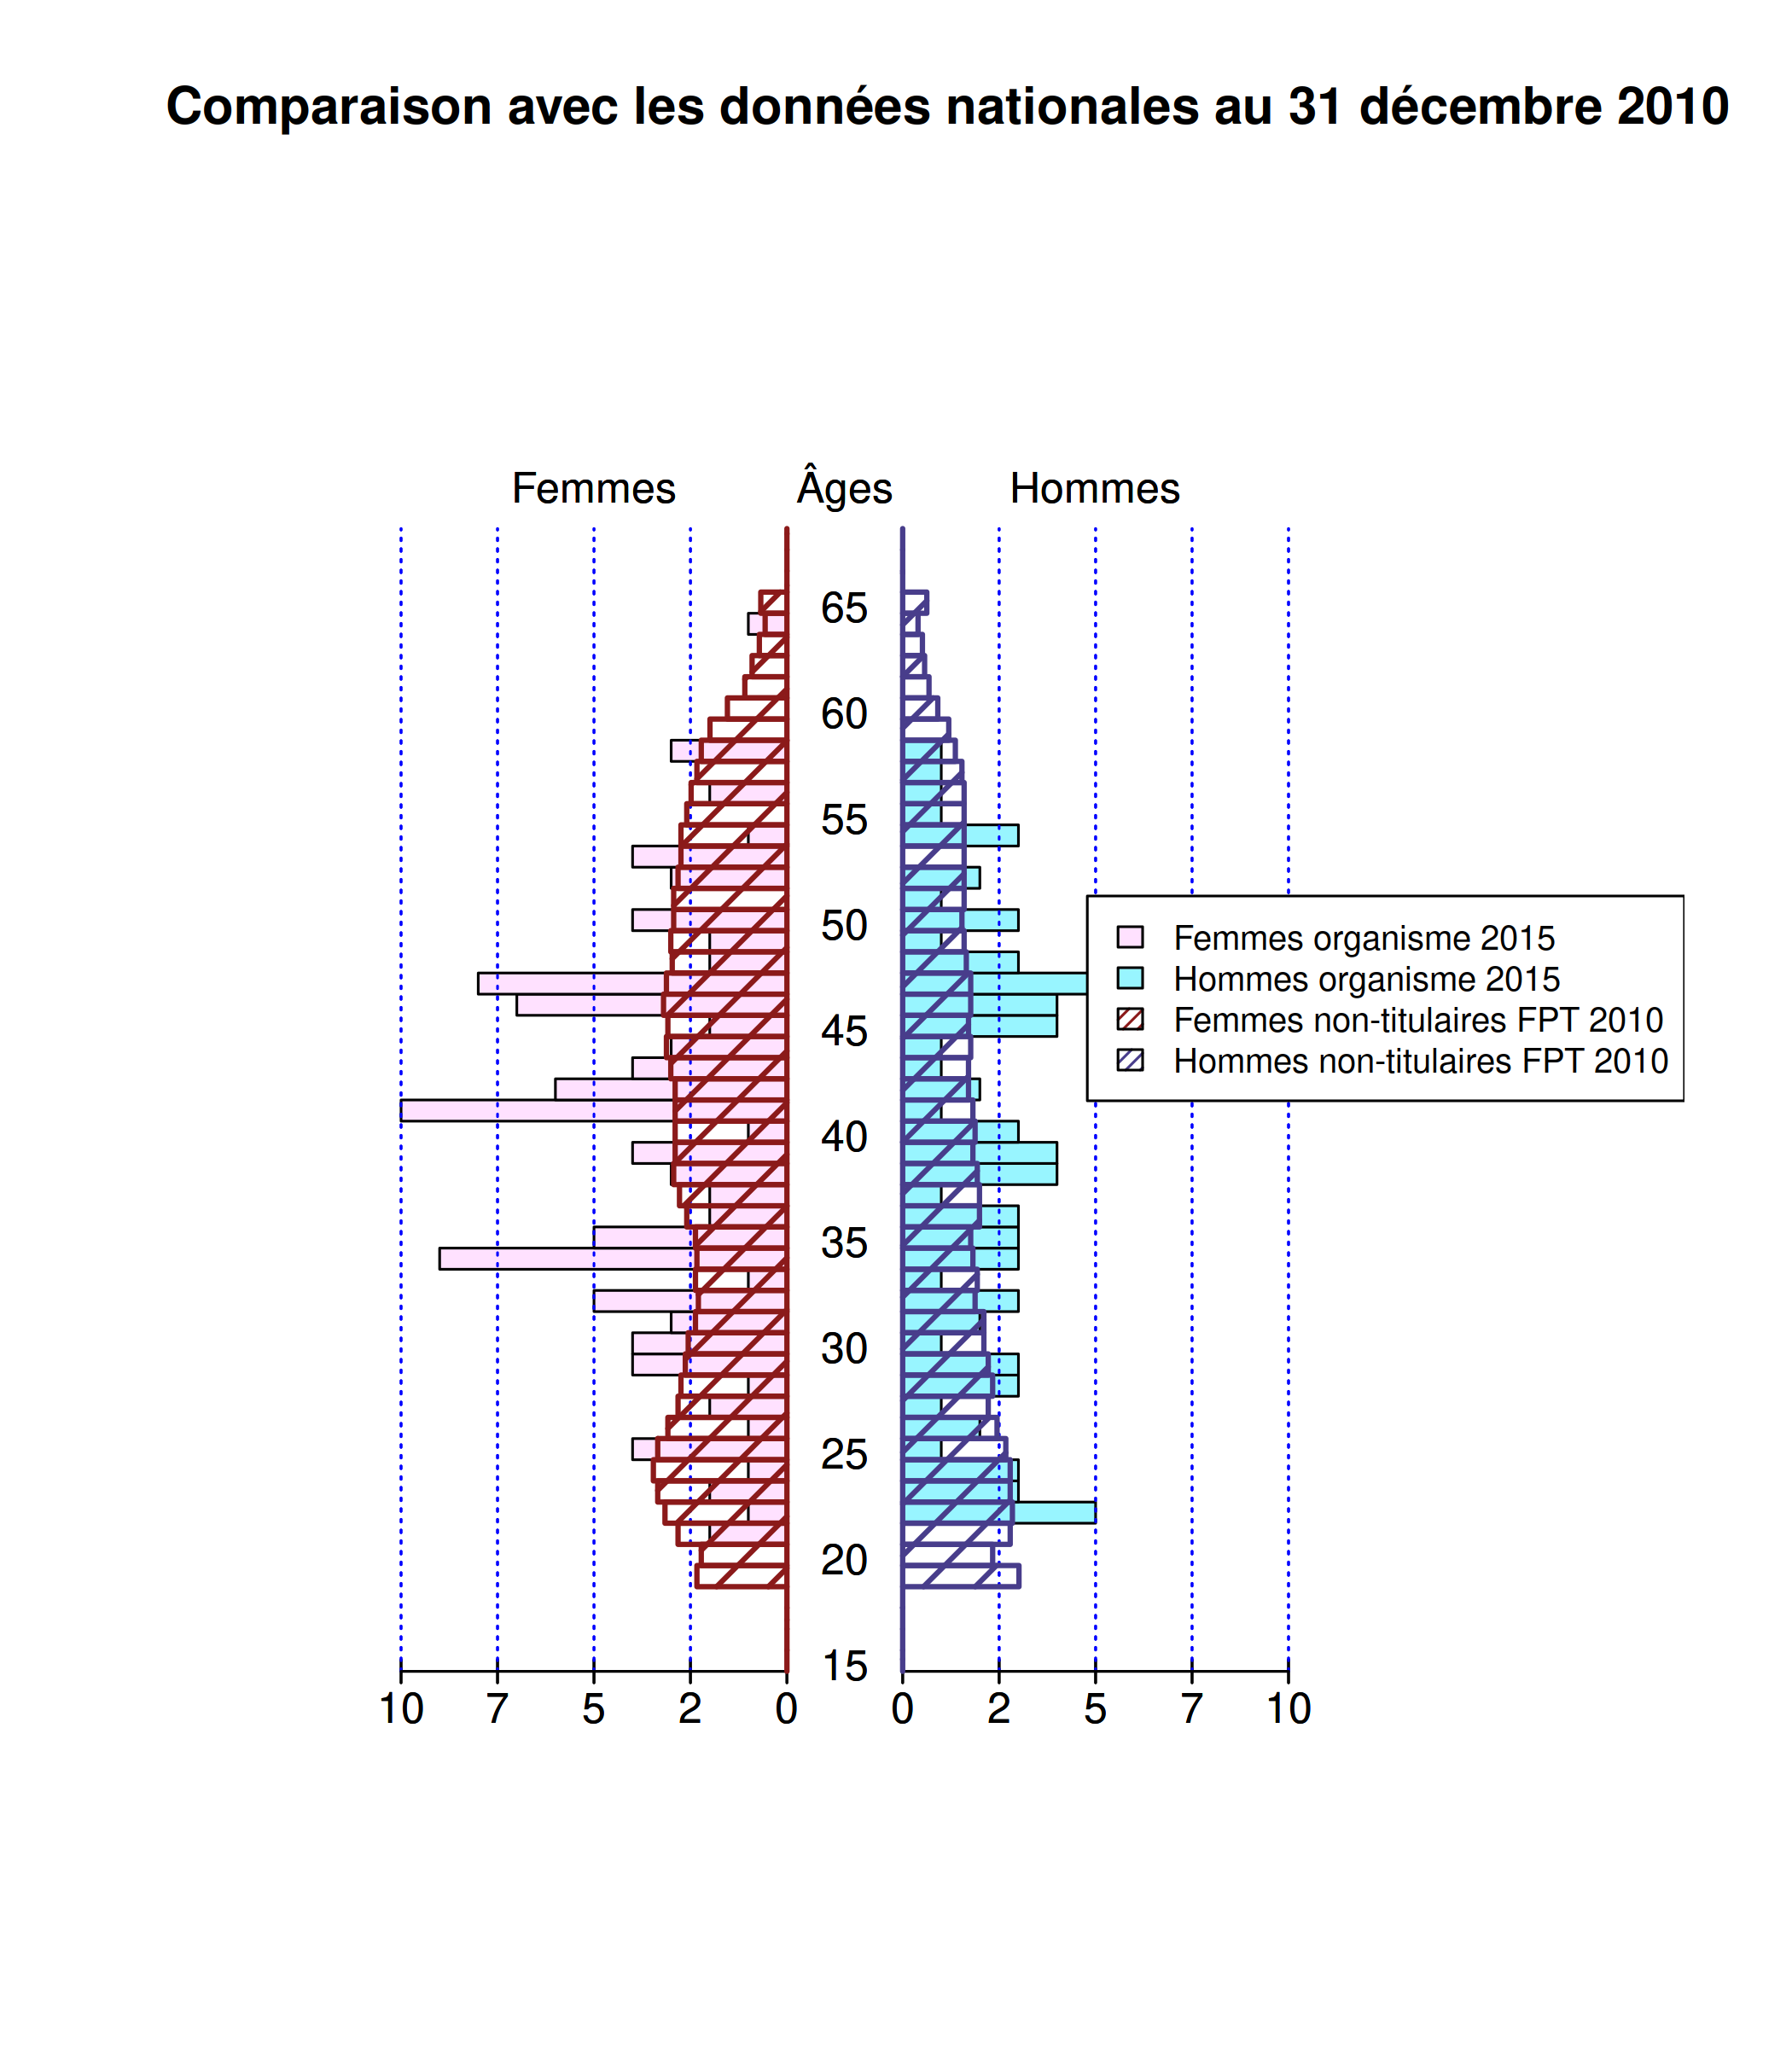
\includegraphics{altair_files/figure-latex/unnamed-chunk-23-2.png} Pour
obtenir les effectifs nationaux, multiplier les abscisses des hommes par
5 314 et les abscisses des femmes par 753\newpage
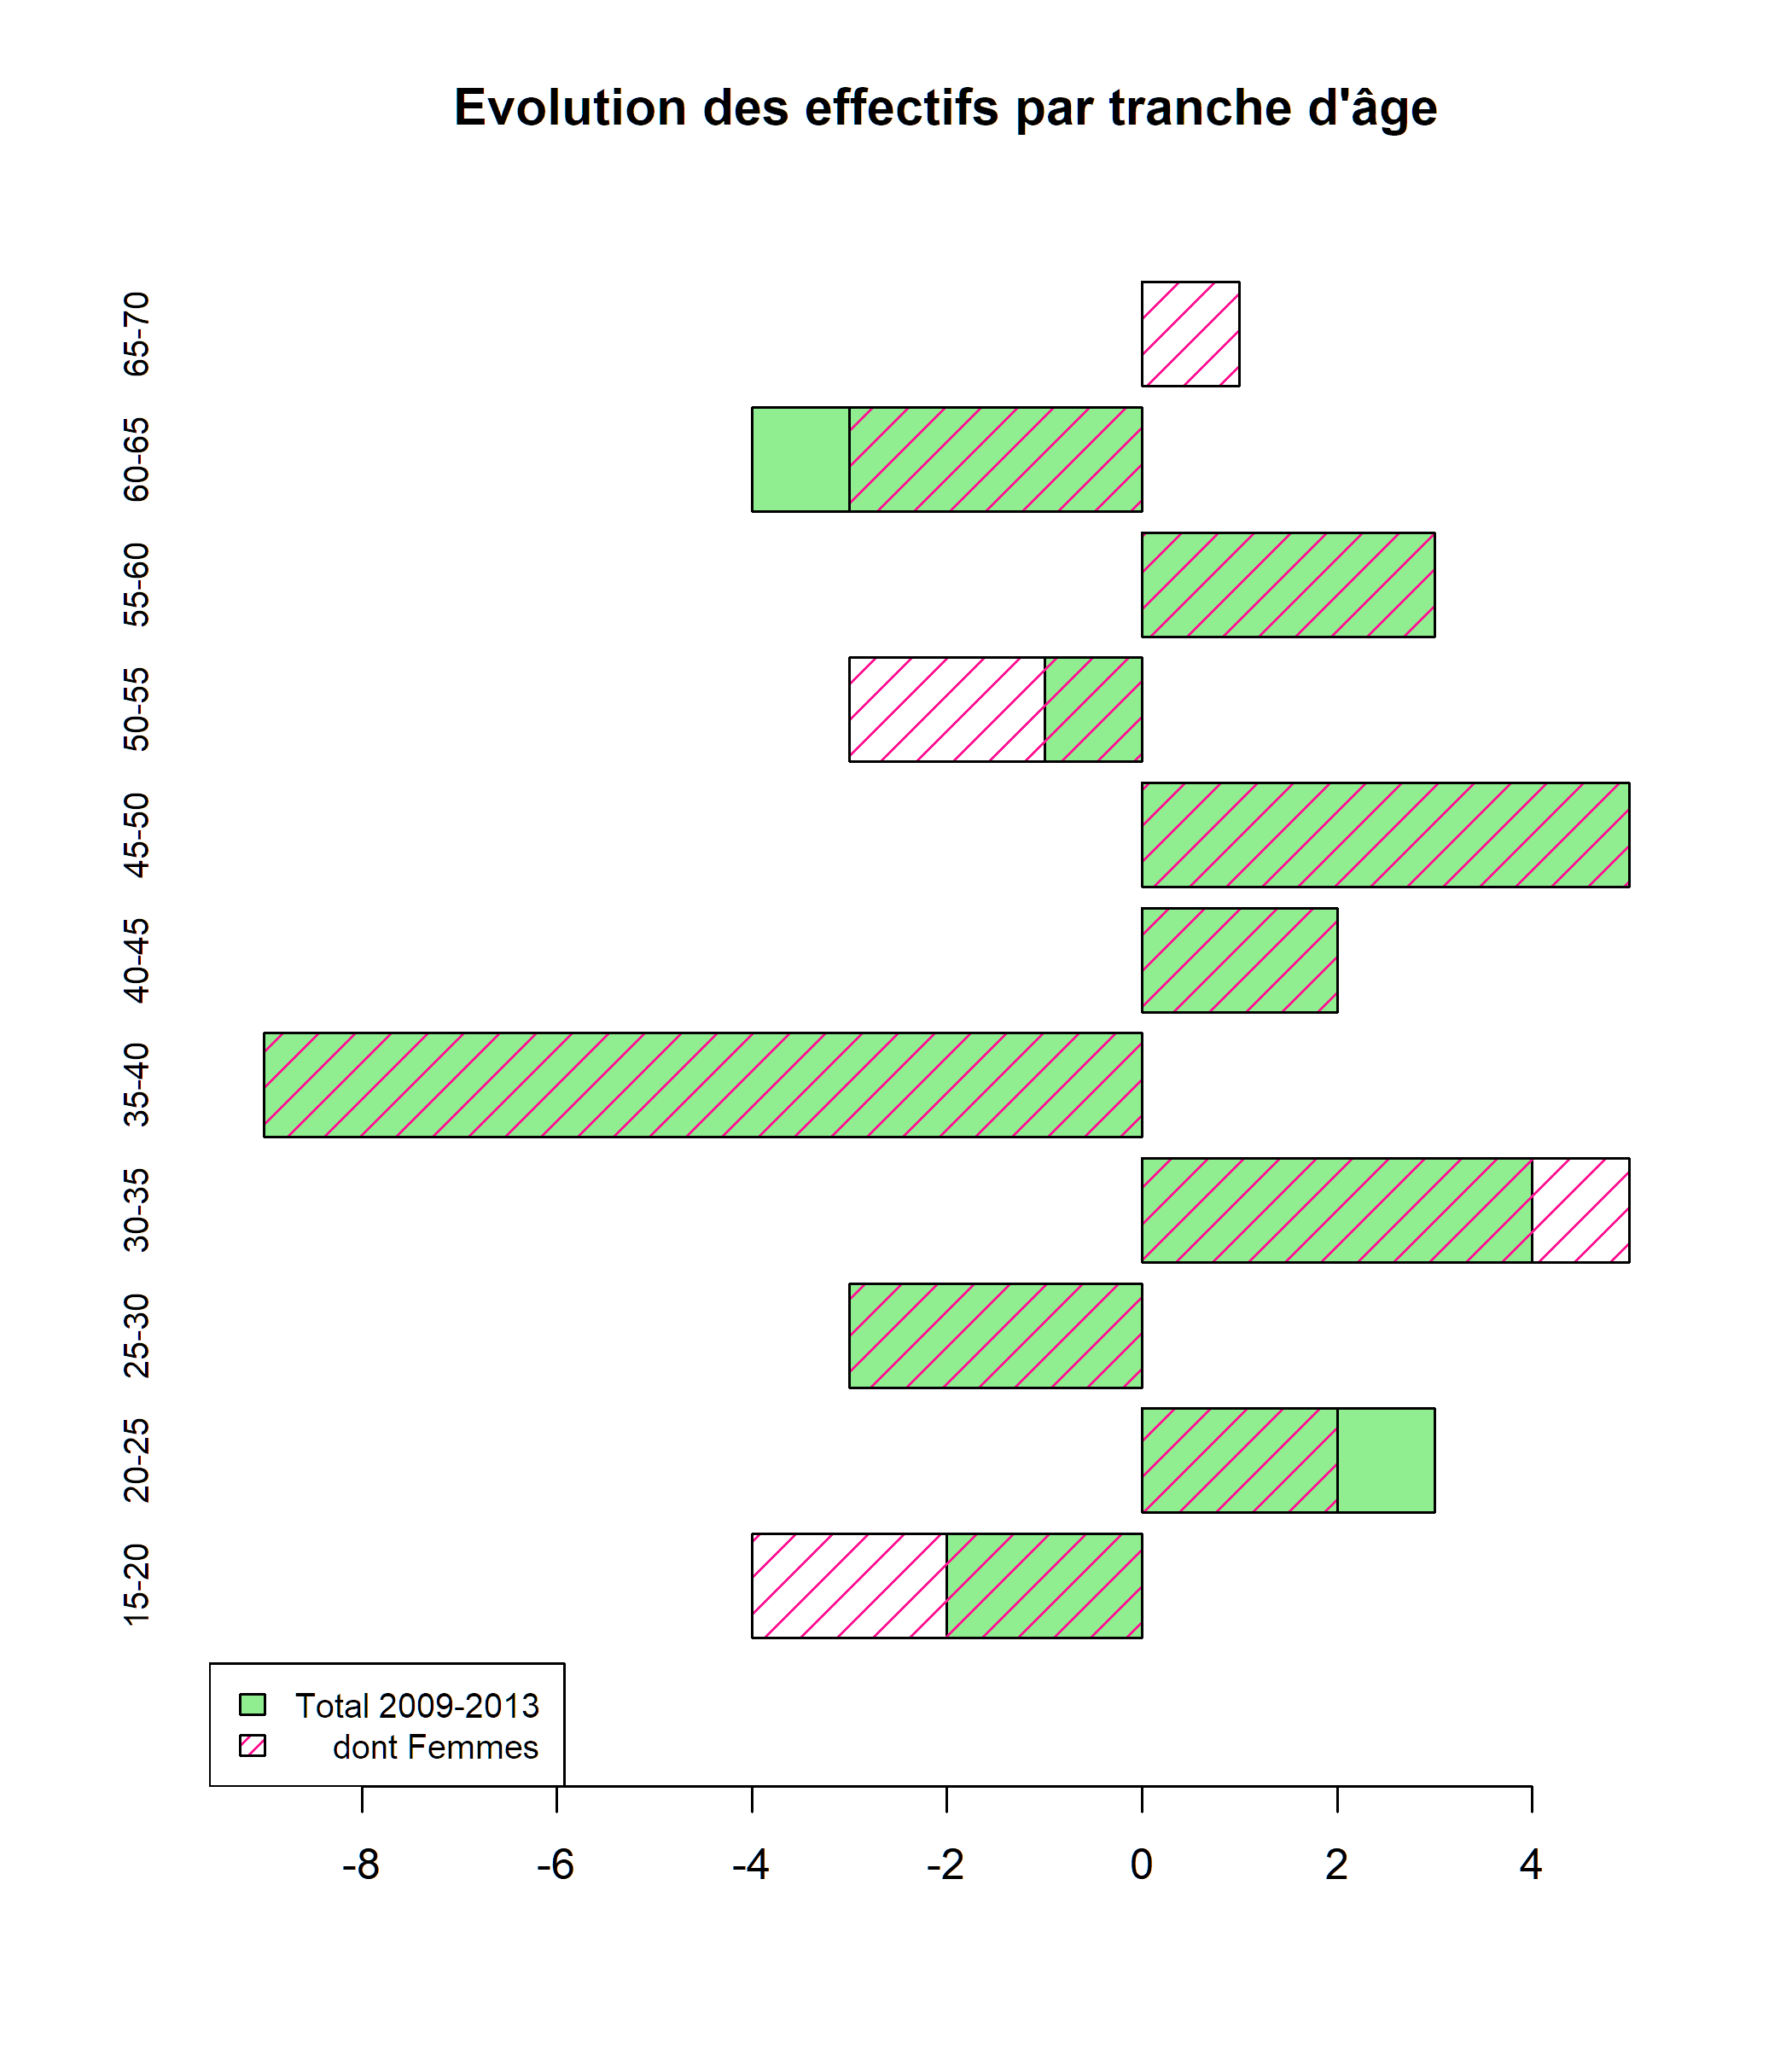
\includegraphics{altair_files/figure-latex/unnamed-chunk-23-3.png}

\href{Docs/Notices/fiche_3.odt}{
\includegraphics{icones/Notice.png}}

\newpage

~\emph{Tableau 1.4.1}

\begin{longtable}[]{@{}ccccc@{}}
\toprule
\begin{minipage}[b]{0.12\columnwidth}\centering
Statistique\strut
\end{minipage} & \begin{minipage}[b]{0.29\columnwidth}\centering
Âge des personnels au 31/12/2009\strut
\end{minipage} & \begin{minipage}[b]{0.08\columnwidth}\centering
Effectif\strut
\end{minipage} & \begin{minipage}[b]{0.29\columnwidth}\centering
Âge des personnels au 31/12/2013\strut
\end{minipage} & \begin{minipage}[b]{0.08\columnwidth}\centering
Effectif\strut
\end{minipage}\tabularnewline
\midrule
\endhead
\begin{minipage}[t]{0.12\columnwidth}\centering
Minimum\strut
\end{minipage} & \begin{minipage}[t]{0.29\columnwidth}\centering
17,0\strut
\end{minipage} & \begin{minipage}[t]{0.08\columnwidth}\centering
\strut
\end{minipage} & \begin{minipage}[t]{0.29\columnwidth}\centering
17,0\strut
\end{minipage} & \begin{minipage}[t]{0.08\columnwidth}\centering
\strut
\end{minipage}\tabularnewline
\begin{minipage}[t]{0.12\columnwidth}\centering
1er quartile\strut
\end{minipage} & \begin{minipage}[t]{0.29\columnwidth}\centering
24,0\strut
\end{minipage} & \begin{minipage}[t]{0.08\columnwidth}\centering
\strut
\end{minipage} & \begin{minipage}[t]{0.29\columnwidth}\centering
23,0\strut
\end{minipage} & \begin{minipage}[t]{0.08\columnwidth}\centering
\strut
\end{minipage}\tabularnewline
\begin{minipage}[t]{0.12\columnwidth}\centering
Médiane\strut
\end{minipage} & \begin{minipage}[t]{0.29\columnwidth}\centering
36,0\strut
\end{minipage} & \begin{minipage}[t]{0.08\columnwidth}\centering
\strut
\end{minipage} & \begin{minipage}[t]{0.29\columnwidth}\centering
35,0\strut
\end{minipage} & \begin{minipage}[t]{0.08\columnwidth}\centering
\strut
\end{minipage}\tabularnewline
\begin{minipage}[t]{0.12\columnwidth}\centering
Moyenne\strut
\end{minipage} & \begin{minipage}[t]{0.29\columnwidth}\centering
36,1\strut
\end{minipage} & \begin{minipage}[t]{0.08\columnwidth}\centering
110\strut
\end{minipage} & \begin{minipage}[t]{0.29\columnwidth}\centering
36,3\strut
\end{minipage} & \begin{minipage}[t]{0.08\columnwidth}\centering
109\strut
\end{minipage}\tabularnewline
\begin{minipage}[t]{0.12\columnwidth}\centering
3ème quartile\strut
\end{minipage} & \begin{minipage}[t]{0.29\columnwidth}\centering
45,8\strut
\end{minipage} & \begin{minipage}[t]{0.08\columnwidth}\centering
\strut
\end{minipage} & \begin{minipage}[t]{0.29\columnwidth}\centering
46,0\strut
\end{minipage} & \begin{minipage}[t]{0.08\columnwidth}\centering
\strut
\end{minipage}\tabularnewline
\begin{minipage}[t]{0.12\columnwidth}\centering
Maximum\strut
\end{minipage} & \begin{minipage}[t]{0.29\columnwidth}\centering
66,0\strut
\end{minipage} & \begin{minipage}[t]{0.08\columnwidth}\centering
\strut
\end{minipage} & \begin{minipage}[t]{0.29\columnwidth}\centering
70,0\strut
\end{minipage} & \begin{minipage}[t]{0.08\columnwidth}\centering
\strut
\end{minipage}\tabularnewline
\bottomrule
\end{longtable}

\href{Bases/Effectifs/Pyramide-des-ages-des-non-titulaires_2009.csv}{Lien
vers la base des âges - début de periode}

\href{Bases/Effectifs/Pyramide-des-ages-des-non-titulaires_2013.csv}{Lien
vers la base des âges - fin de periode}

\href{Docs/Notices/fiche_1.odt}{
\includegraphics{icones/Notice.png}}

\hypertarget{pyramide-des-ages-autres-statuts}{%
\subsection{1.5 Pyramide des âges, autres statuts
~}\label{pyramide-des-ages-autres-statuts}}

\href{Docs/Notices/fiche_2.odt}{
\includegraphics{icones/Notice.png}}

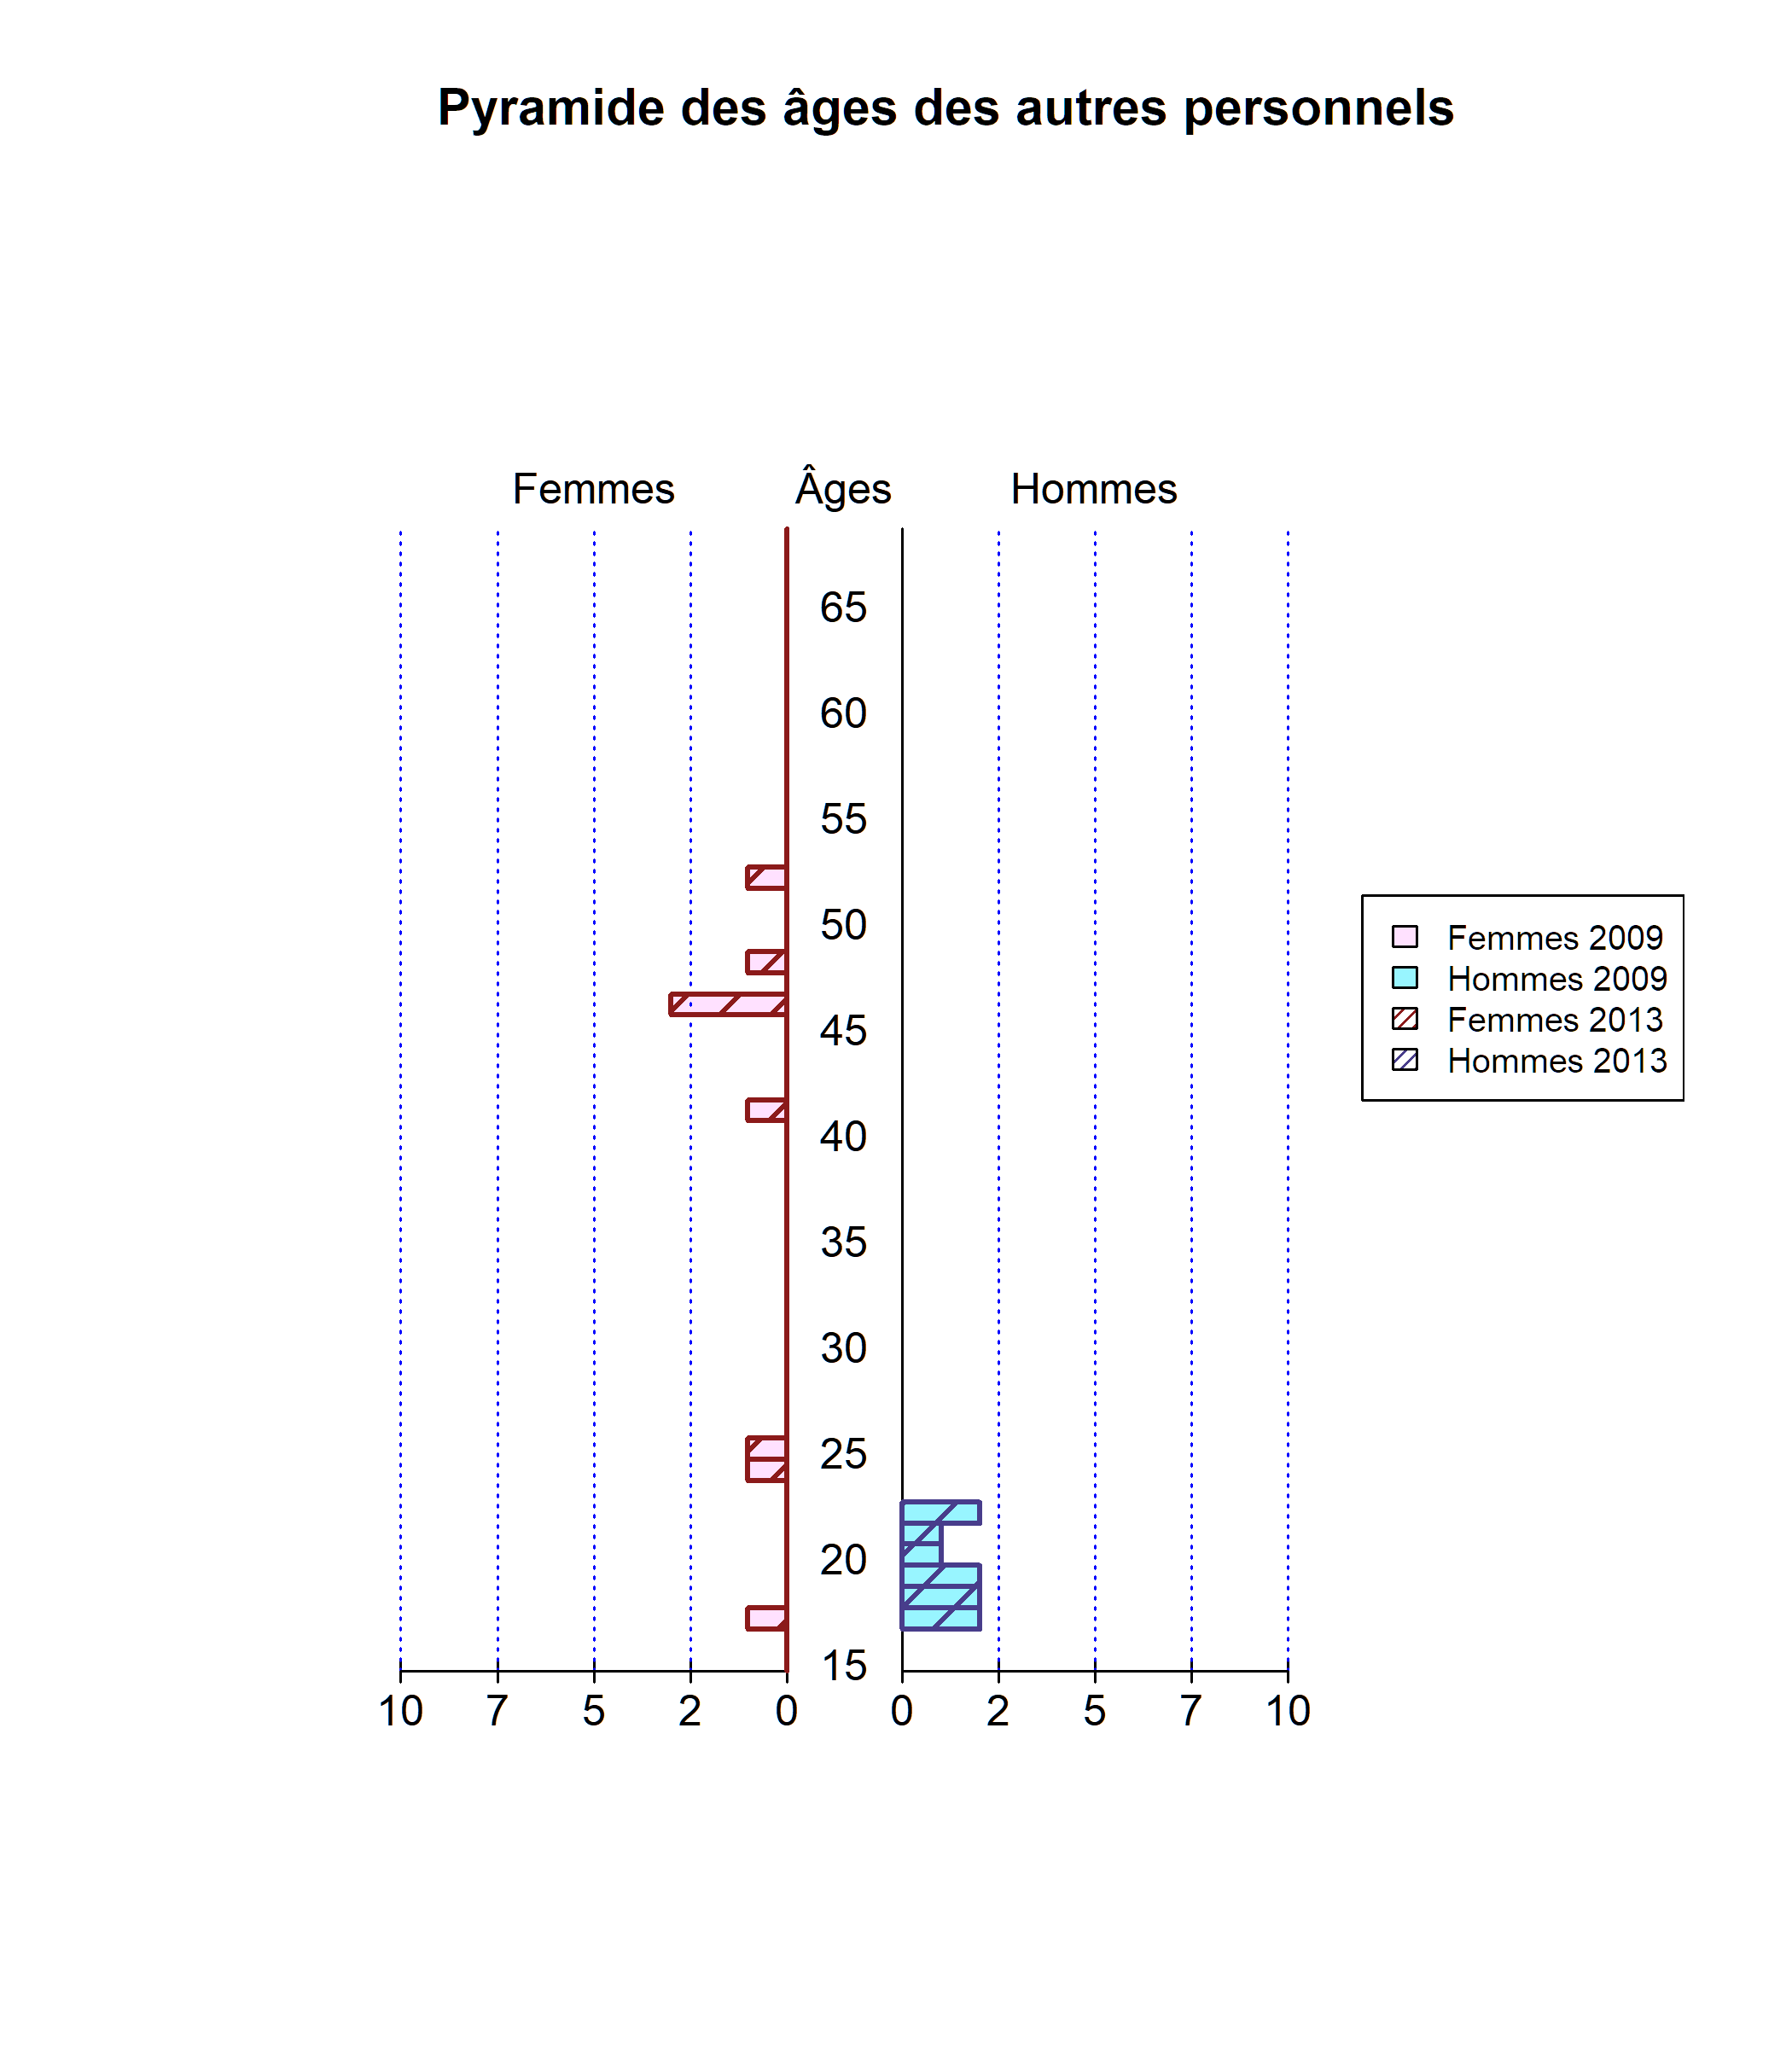
\includegraphics{altair_files/figure-latex/unnamed-chunk-29-1.png} La
pyramide des âges de début de periode ne peut être produite. \newpage Le
graphique des variations d'effectifs par tranche d'âge ne peut être
produit.

\href{Docs/Notices/fiche_3.odt}{
\includegraphics{icones/Notice.png}}

\newpage

~\emph{Tableau 1.5.1}

\begin{longtable}[]{@{}ccccc@{}}
\toprule
\begin{minipage}[b]{0.12\columnwidth}\centering
Statistique\strut
\end{minipage} & \begin{minipage}[b]{0.29\columnwidth}\centering
Âge des personnels au 31/12/2009\strut
\end{minipage} & \begin{minipage}[b]{0.08\columnwidth}\centering
Effectif\strut
\end{minipage} & \begin{minipage}[b]{0.29\columnwidth}\centering
Âge des personnels au 31/12/2013\strut
\end{minipage} & \begin{minipage}[b]{0.08\columnwidth}\centering
Effectif\strut
\end{minipage}\tabularnewline
\midrule
\endhead
\begin{minipage}[t]{0.12\columnwidth}\centering
Minimum\strut
\end{minipage} & \begin{minipage}[t]{0.29\columnwidth}\centering
16,0\strut
\end{minipage} & \begin{minipage}[t]{0.08\columnwidth}\centering
\strut
\end{minipage} & \begin{minipage}[t]{0.29\columnwidth}\centering
17,0\strut
\end{minipage} & \begin{minipage}[t]{0.08\columnwidth}\centering
\strut
\end{minipage}\tabularnewline
\begin{minipage}[t]{0.12\columnwidth}\centering
1er quartile\strut
\end{minipage} & \begin{minipage}[t]{0.29\columnwidth}\centering
21,8\strut
\end{minipage} & \begin{minipage}[t]{0.08\columnwidth}\centering
\strut
\end{minipage} & \begin{minipage}[t]{0.29\columnwidth}\centering
18,5\strut
\end{minipage} & \begin{minipage}[t]{0.08\columnwidth}\centering
\strut
\end{minipage}\tabularnewline
\begin{minipage}[t]{0.12\columnwidth}\centering
Médiane\strut
\end{minipage} & \begin{minipage}[t]{0.29\columnwidth}\centering
48,5\strut
\end{minipage} & \begin{minipage}[t]{0.08\columnwidth}\centering
\strut
\end{minipage} & \begin{minipage}[t]{0.29\columnwidth}\centering
22,0\strut
\end{minipage} & \begin{minipage}[t]{0.08\columnwidth}\centering
\strut
\end{minipage}\tabularnewline
\begin{minipage}[t]{0.12\columnwidth}\centering
Moyenne\strut
\end{minipage} & \begin{minipage}[t]{0.29\columnwidth}\centering
41,9\strut
\end{minipage} & \begin{minipage}[t]{0.08\columnwidth}\centering
22\strut
\end{minipage} & \begin{minipage}[t]{0.29\columnwidth}\centering
28,3\strut
\end{minipage} & \begin{minipage}[t]{0.08\columnwidth}\centering
19\strut
\end{minipage}\tabularnewline
\begin{minipage}[t]{0.12\columnwidth}\centering
3ème quartile\strut
\end{minipage} & \begin{minipage}[t]{0.29\columnwidth}\centering
56,0\strut
\end{minipage} & \begin{minipage}[t]{0.08\columnwidth}\centering
\strut
\end{minipage} & \begin{minipage}[t]{0.29\columnwidth}\centering
43,5\strut
\end{minipage} & \begin{minipage}[t]{0.08\columnwidth}\centering
\strut
\end{minipage}\tabularnewline
\begin{minipage}[t]{0.12\columnwidth}\centering
Maximum\strut
\end{minipage} & \begin{minipage}[t]{0.29\columnwidth}\centering
60,0\strut
\end{minipage} & \begin{minipage}[t]{0.08\columnwidth}\centering
\strut
\end{minipage} & \begin{minipage}[t]{0.29\columnwidth}\centering
52,0\strut
\end{minipage} & \begin{minipage}[t]{0.08\columnwidth}\centering
\strut
\end{minipage}\tabularnewline
\bottomrule
\end{longtable}

\href{Bases/Effectifs/Pyramide-des-ages-des-autres-personnels_2009.csv}{Lien
vers la base des âges - début de periode}

\href{Bases/Effectifs/Pyramide-des-ages-des-autres-personnels_2013.csv}{Lien
vers la base des âges - fin de periode}

\href{Docs/Notices/fiche_1.odt}{
\includegraphics{icones/Notice.png}}

\emph{Source des comparaisons avec les données nationales}

Rapport annuel sur l'état de la fonction publique pour 2016\\
\href{Docs/insee_pyramide_fph_2013.csv}{Pyramide 2013 FPH}\\
\href{Docs/insee_pyramide_fpt_2013.csv}{Pyramide 2013 FPT}\\
\emph{Toutes les pyramides des âges sont établies au 31 décembre de
l'annee considérée.}\\
\emph{Les élus ne sont pas compris dans le périmètre statistique.}

\hypertarget{effectifs-des-personnels-par-duree-de-service}{%
\subsection{1.6 Effectifs des personnels par duree de
service}\label{effectifs-des-personnels-par-duree-de-service}}

\textbf{Personnels en fonction (hors élus) des exercices 2009 à 2013
inclus :}

~\emph{Tableau 1.6.1}

\begin{longtable}[]{@{}cccc@{}}
\toprule
Plus de 2 ans & Moins de 2 ans & Moins d'un an & Moins de six
mois\tabularnewline
\midrule
\endhead
2 185 & 195 & 88 & 23\tabularnewline
\bottomrule
\end{longtable}

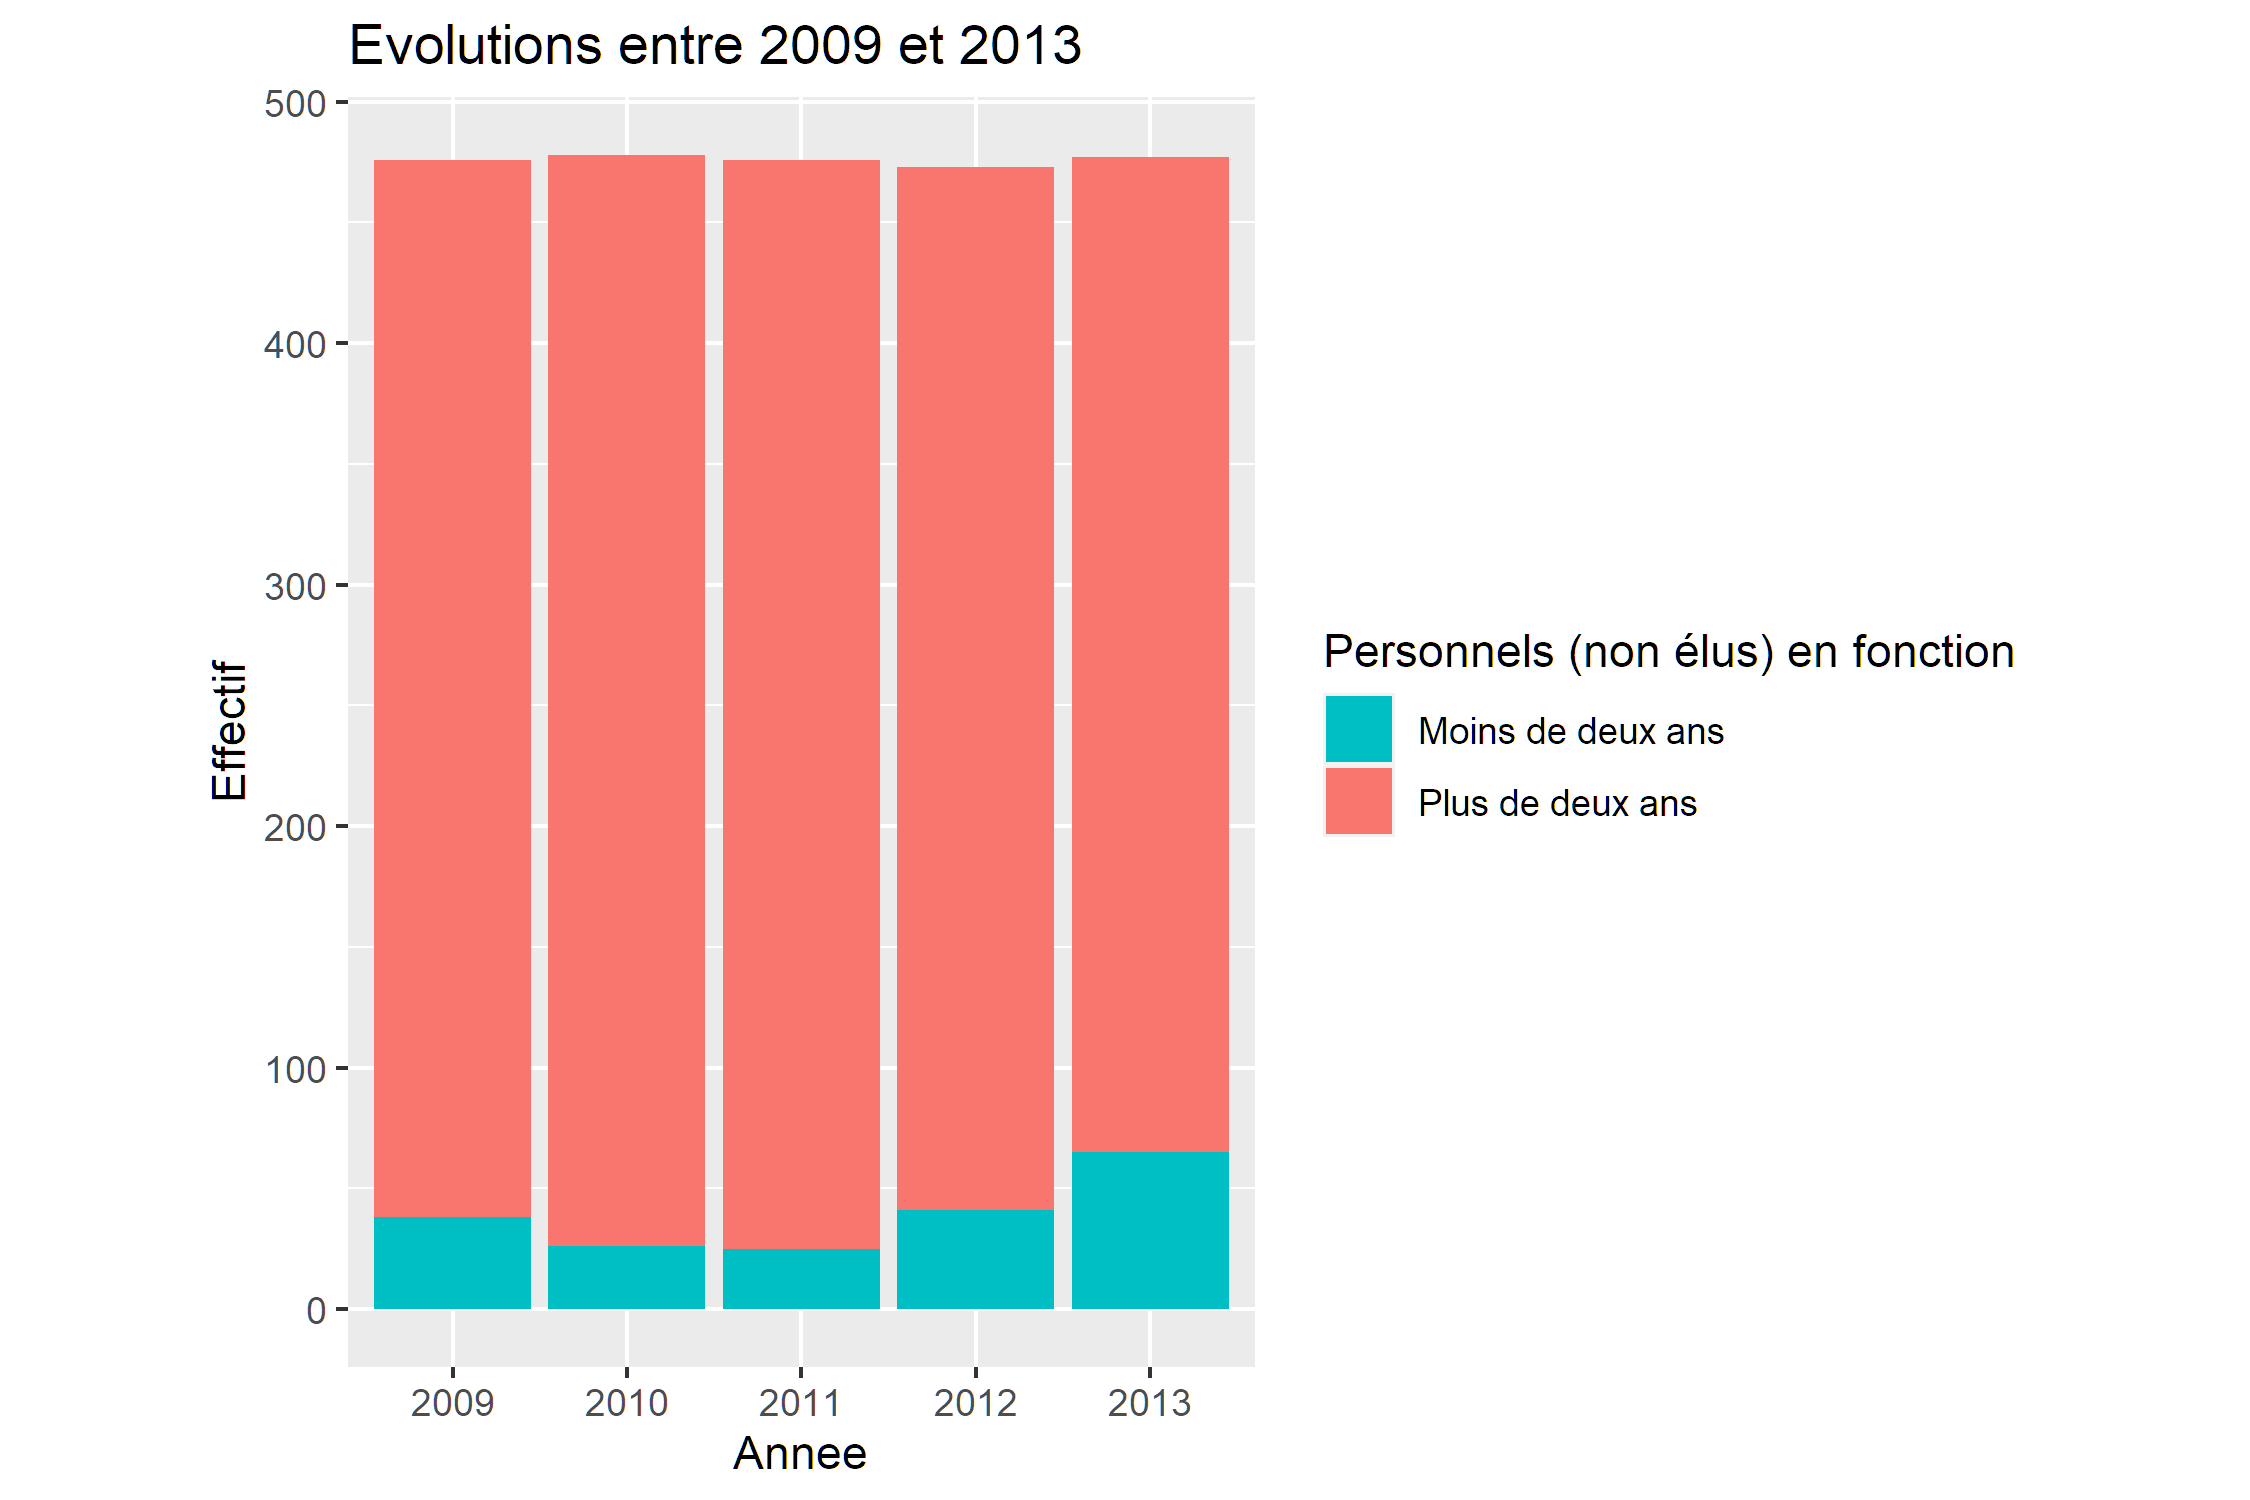
\includegraphics{altair_files/figure-latex/unnamed-chunk-35-1.png}

\textbf{Effectifs (hors élus)}

~\emph{Tableau 1.6.2}

\begin{longtable}[]{@{}lccccc@{}}
\toprule
& 2009 & 2010 & 2011 & 2012 & 2013\tabularnewline
\midrule
\endhead
Plus de deux ans & 438 & 452 & 451 & 432 & 412\tabularnewline
Moins de deux ans & 38 & 26 & 25 & 41 & 65\tabularnewline
Total & 476 & 478 & 476 & 473 & 477\tabularnewline
\bottomrule
\end{longtable}

\textbf{Nota :} \emph{Personnels en place : ayant servi au moins deux
années consécutives pendant la periode.}\\
\emph{Plus/moins de deux ans : plus/mois de 730 jours sur la periode
sous revue.}

\hypertarget{remunerations-brutes-analyse-pour-le-premier-exercice}{%
\section{2. Rémunérations brutes : analyse pour le premier
exercice}\label{remunerations-brutes-analyse-pour-le-premier-exercice}}

\textbf{Exercice : 2009 }

\hypertarget{masse-salariale-brute-de-lensemble-des-agents}{%
\subsection{2.1 Masse salariale brute de l'ensemble des
agents}\label{masse-salariale-brute-de-lensemble-des-agents}}

\textbf{Cumuls des rémunérations brutes pour l'exercice 2009 }

\emph{Personnels (hors élus)}

~\emph{Tableau 2.1.1}

\begin{longtable}[]{@{}ll@{}}
\toprule
Agrégats & k€\tabularnewline
\midrule
\endhead
Brut annuel (bulletins) & 10 647 917,6\tabularnewline
Brut annuel (lignes) : & 10 649 898,0\tabularnewline
~dont ~Primes : & 1 508 455,9\tabularnewline
~dont ~Autres rémunérations &\tabularnewline
Part de primes en \% & 14,2\tabularnewline
\bottomrule
\end{longtable}

\textbf{Définitions :}

\emph{Brut annuel (bulletins)} : somme du champ \emph{Brut}\\
\emph{Brut annuel (lignes)} : somme du champ \emph{Montant} des lignes
de paye, dont :\\
\emph{Primes} : indemnités sauf remboursements, certaines IJSS,
indemnités d'élu le cas échéant, Supplément familial de traitement et
Indemnité de résidence\\
\emph{Autres rémunérations} : acomptes, retenues sur brut, rémunérations
diverses, rappels

\textbf{Tests de cohérence}

Somme des rémunérations brutes versées aux personnels (non élus) :

~\emph{Tableau 2.1.2}

\begin{longtable}[]{@{}ll@{}}
\toprule
Agrégats & k€\tabularnewline
\midrule
\endhead
Bulletins de paie & 10 647 917,6\tabularnewline
Lignes de paie & 10 649 898,0\tabularnewline
Difference & -1 980,4\tabularnewline
\bottomrule
\end{longtable}

à comparer aux soldes des comptes 641 et 648 du compte de gestion.

\hypertarget{masse-salariale-brute-des-fonctionnaires}{%
\subsection{2.2 Masse salariale brute des
fonctionnaires}\label{masse-salariale-brute-des-fonctionnaires}}

\emph{Cette section concerne les personnels fonctionnaires titulaires et
stagiaires}

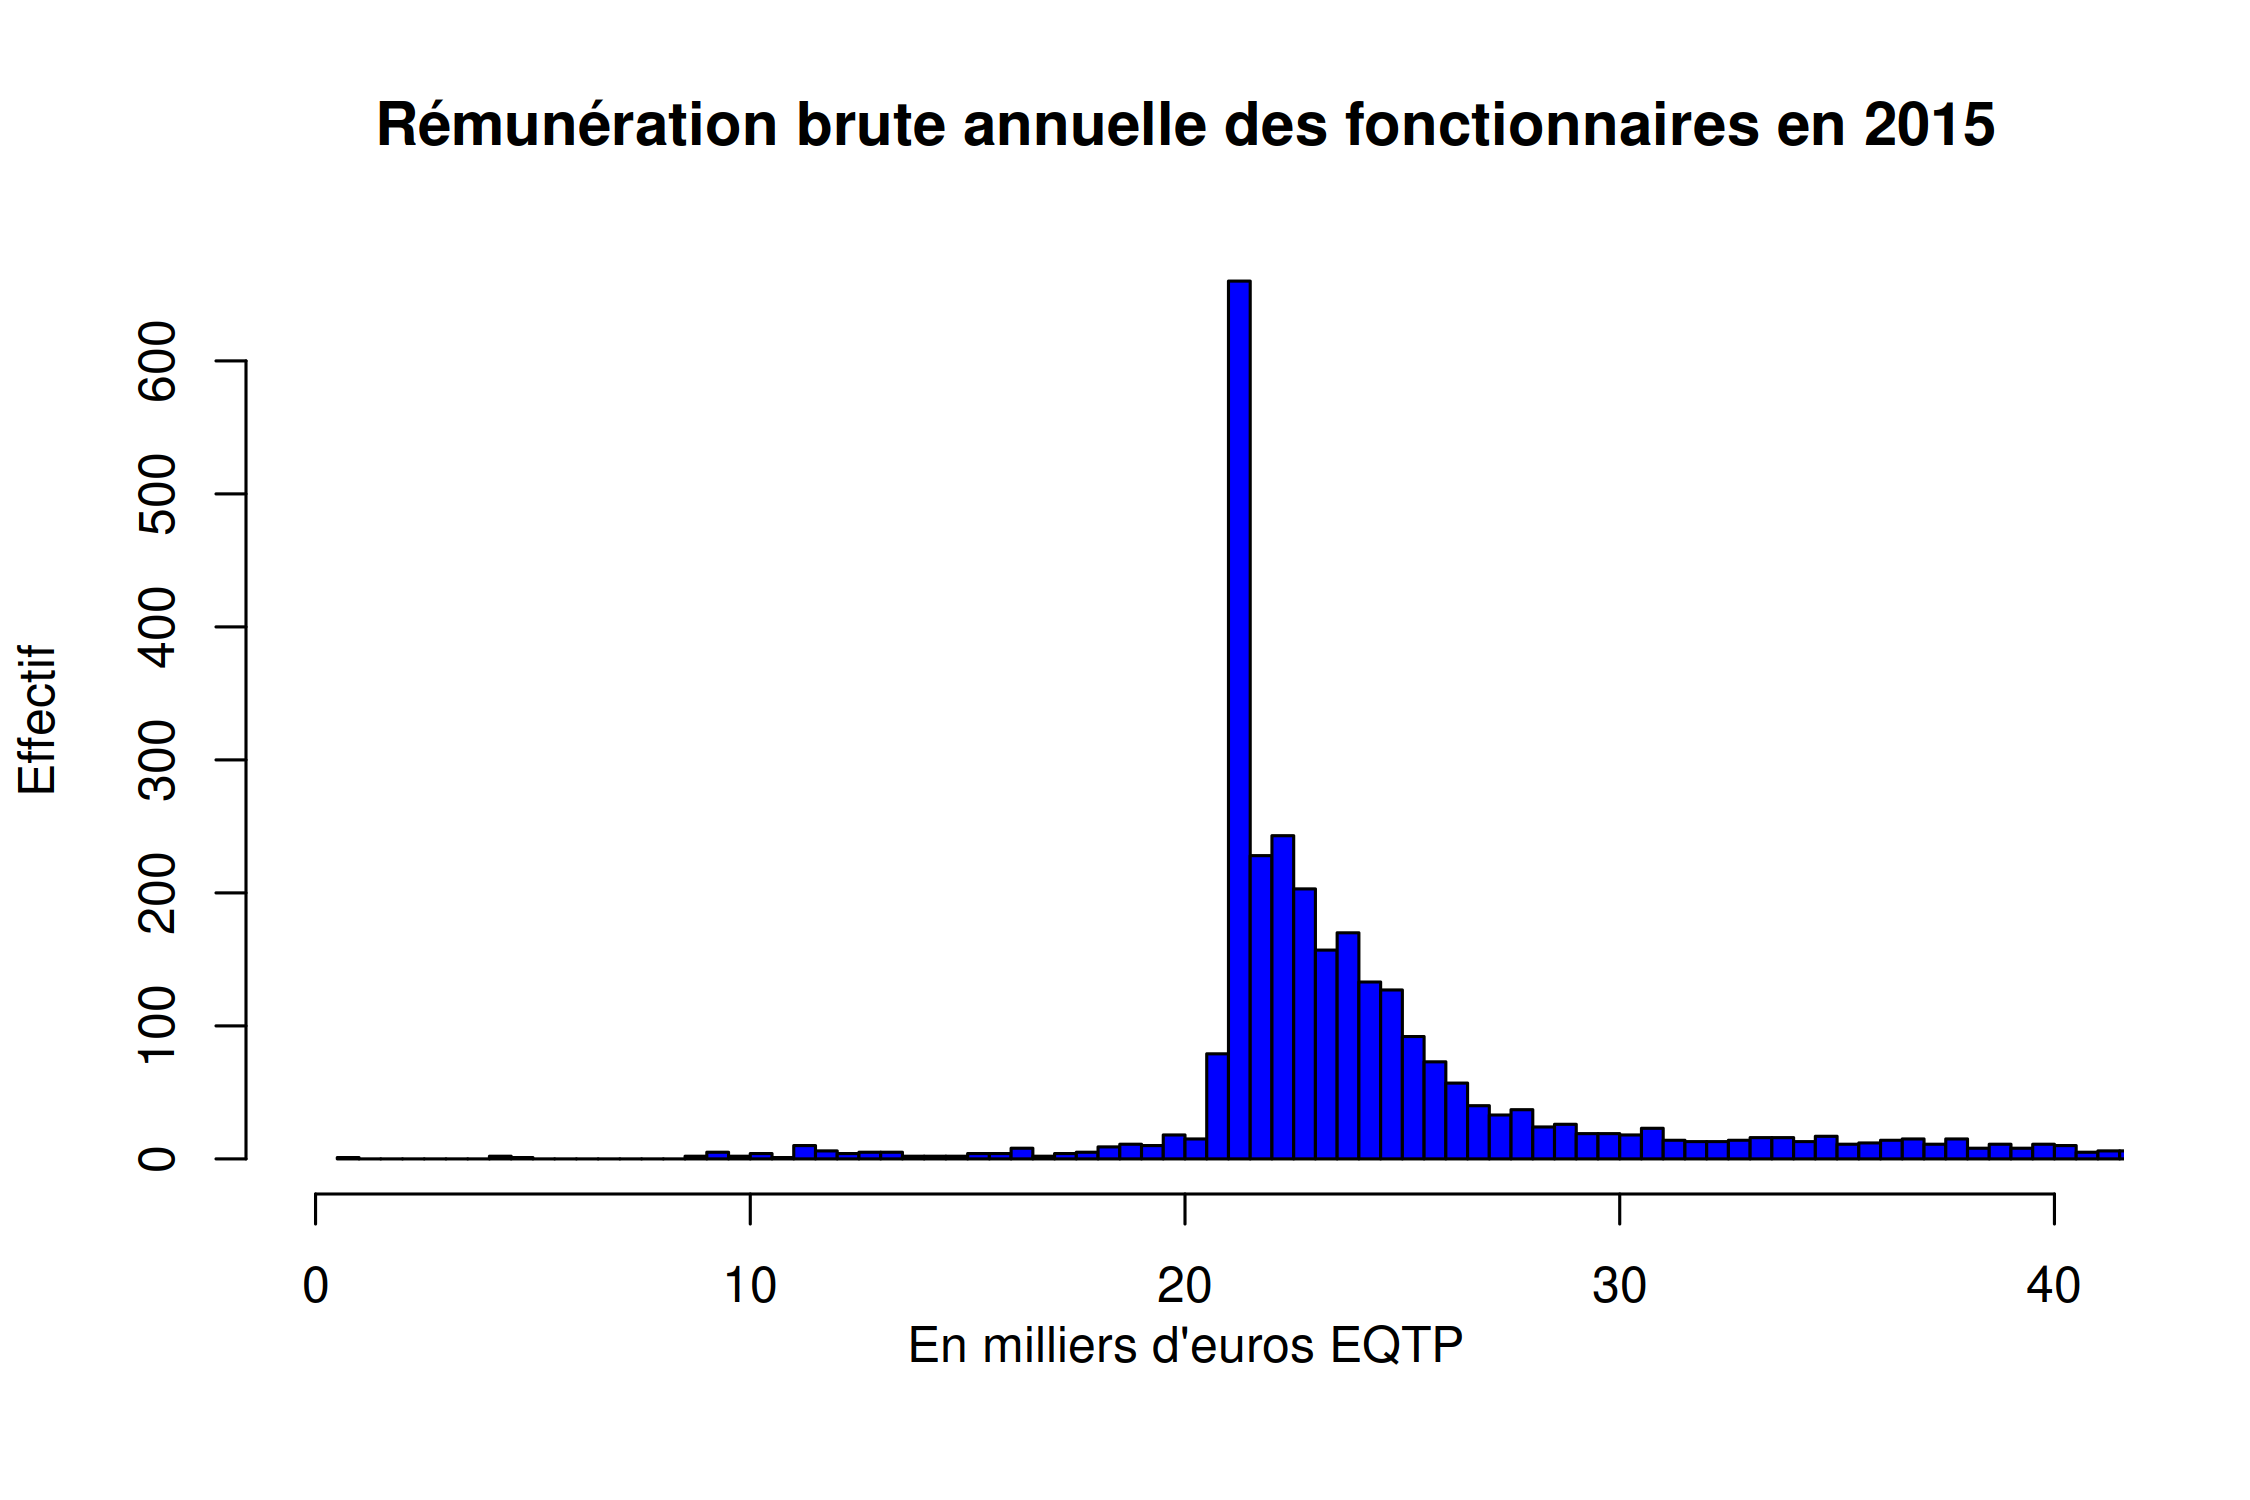
\includegraphics{altair_files/figure-latex/unnamed-chunk-43-1.png}

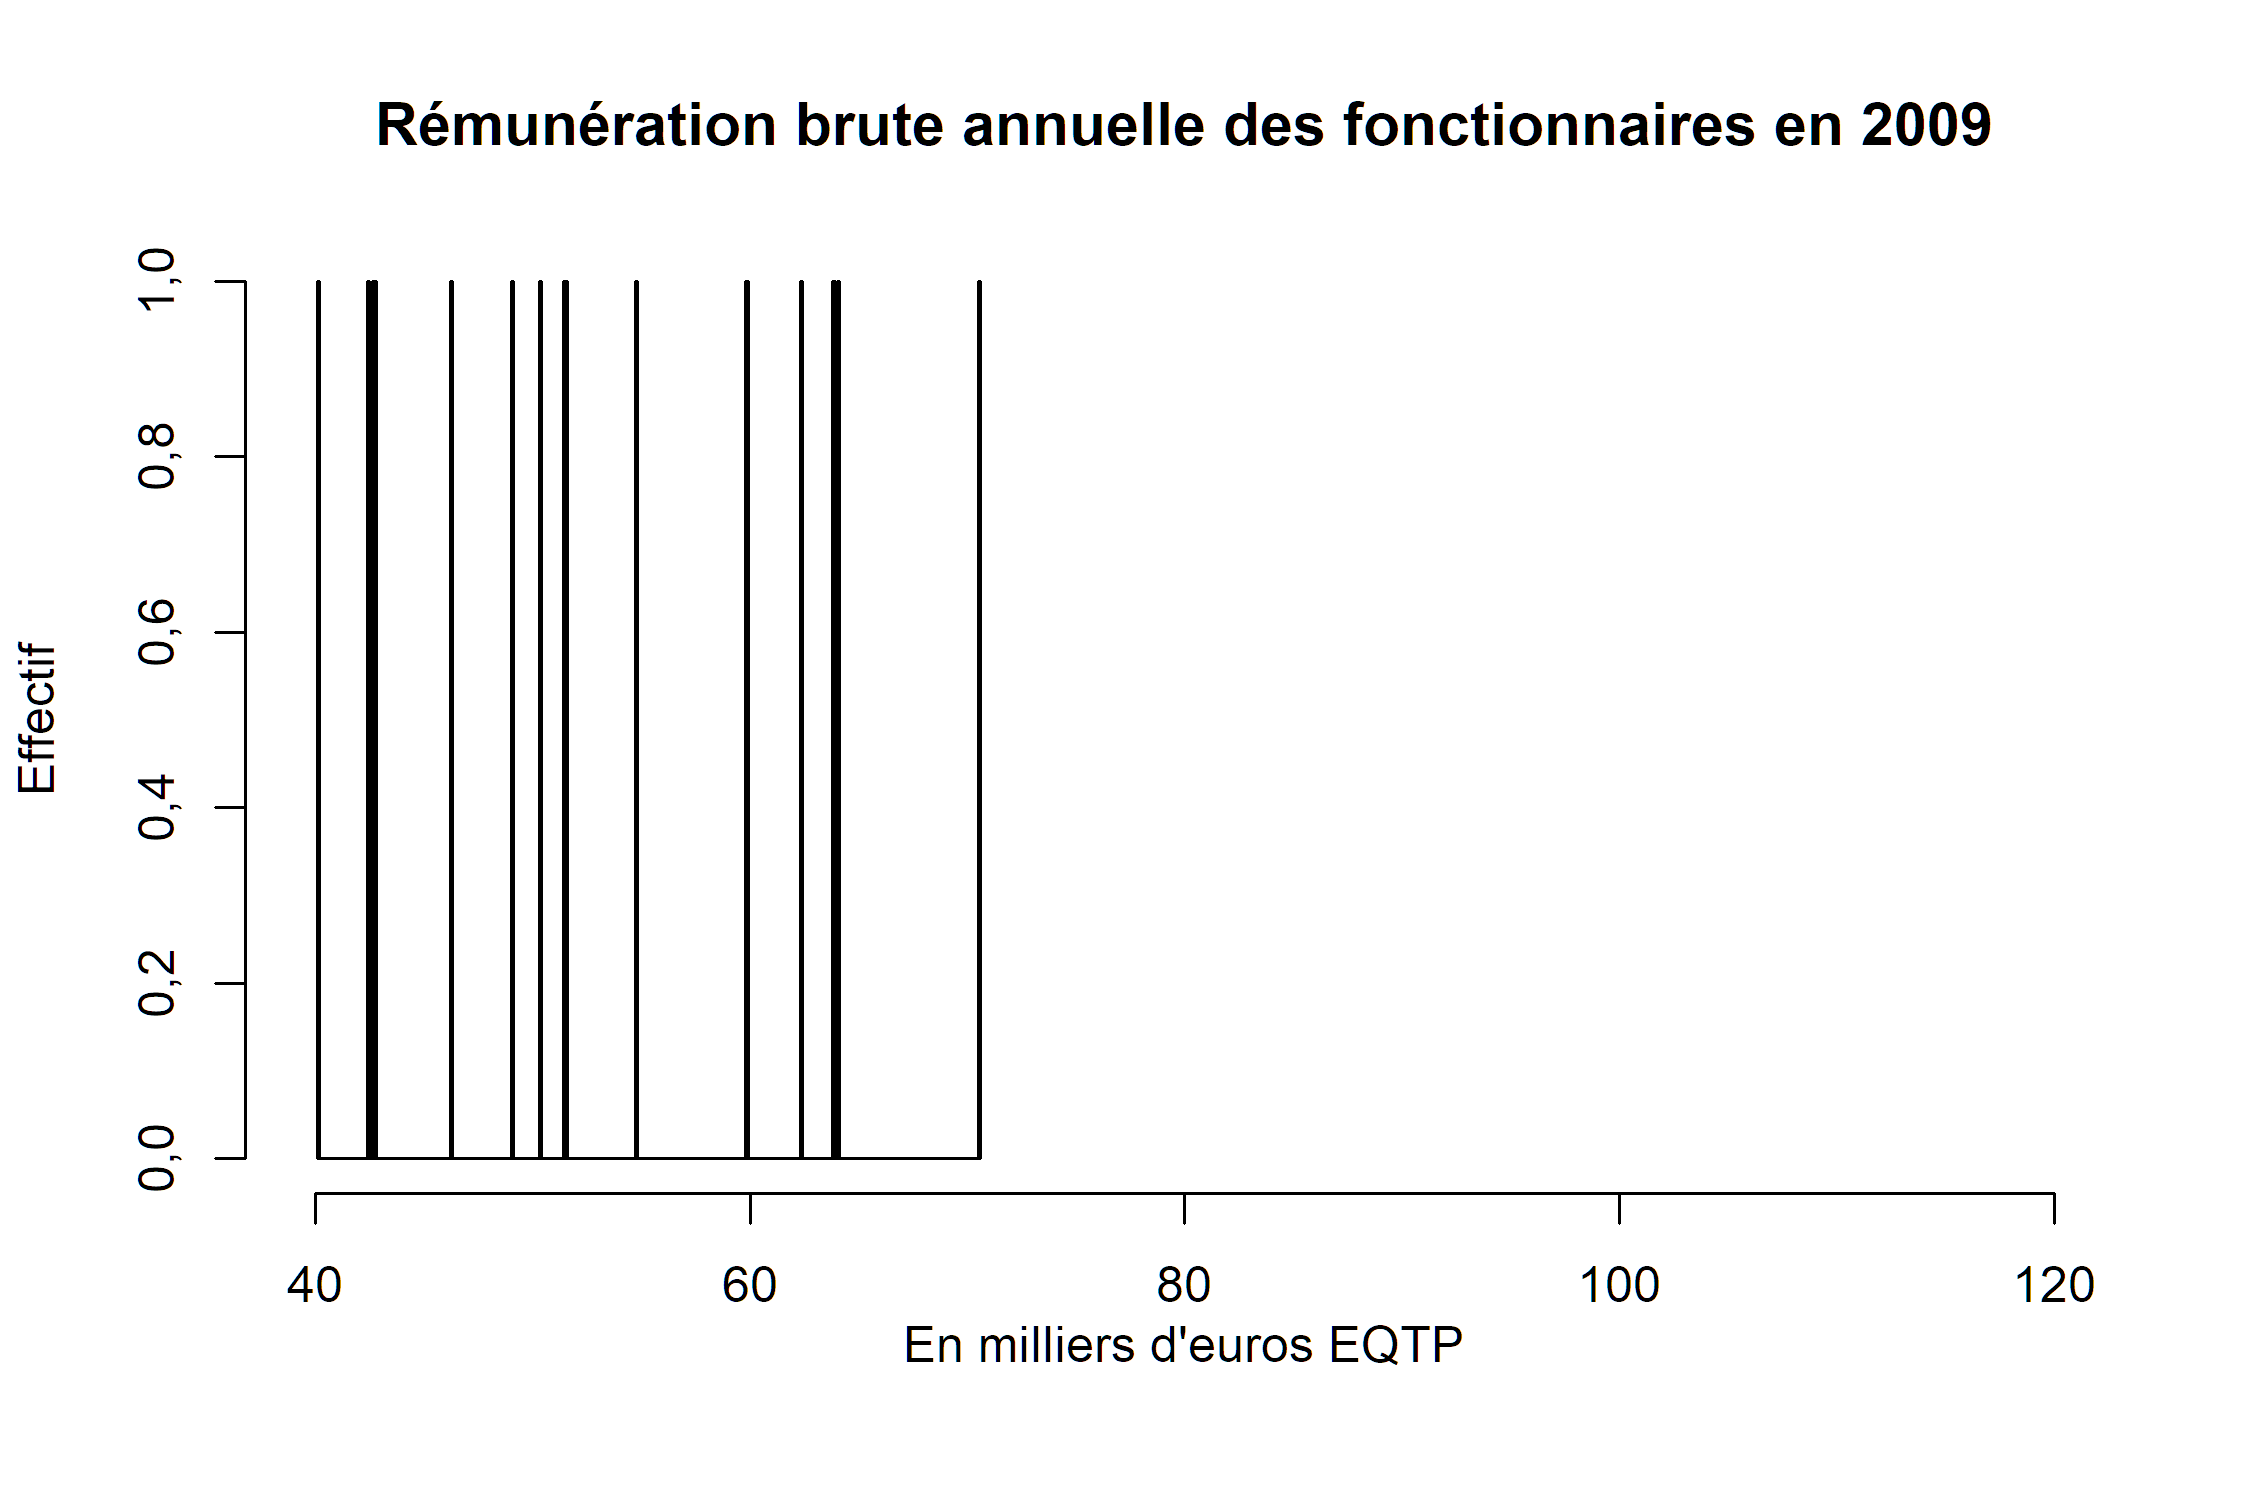
\includegraphics{altair_files/figure-latex/unnamed-chunk-43-2.png}

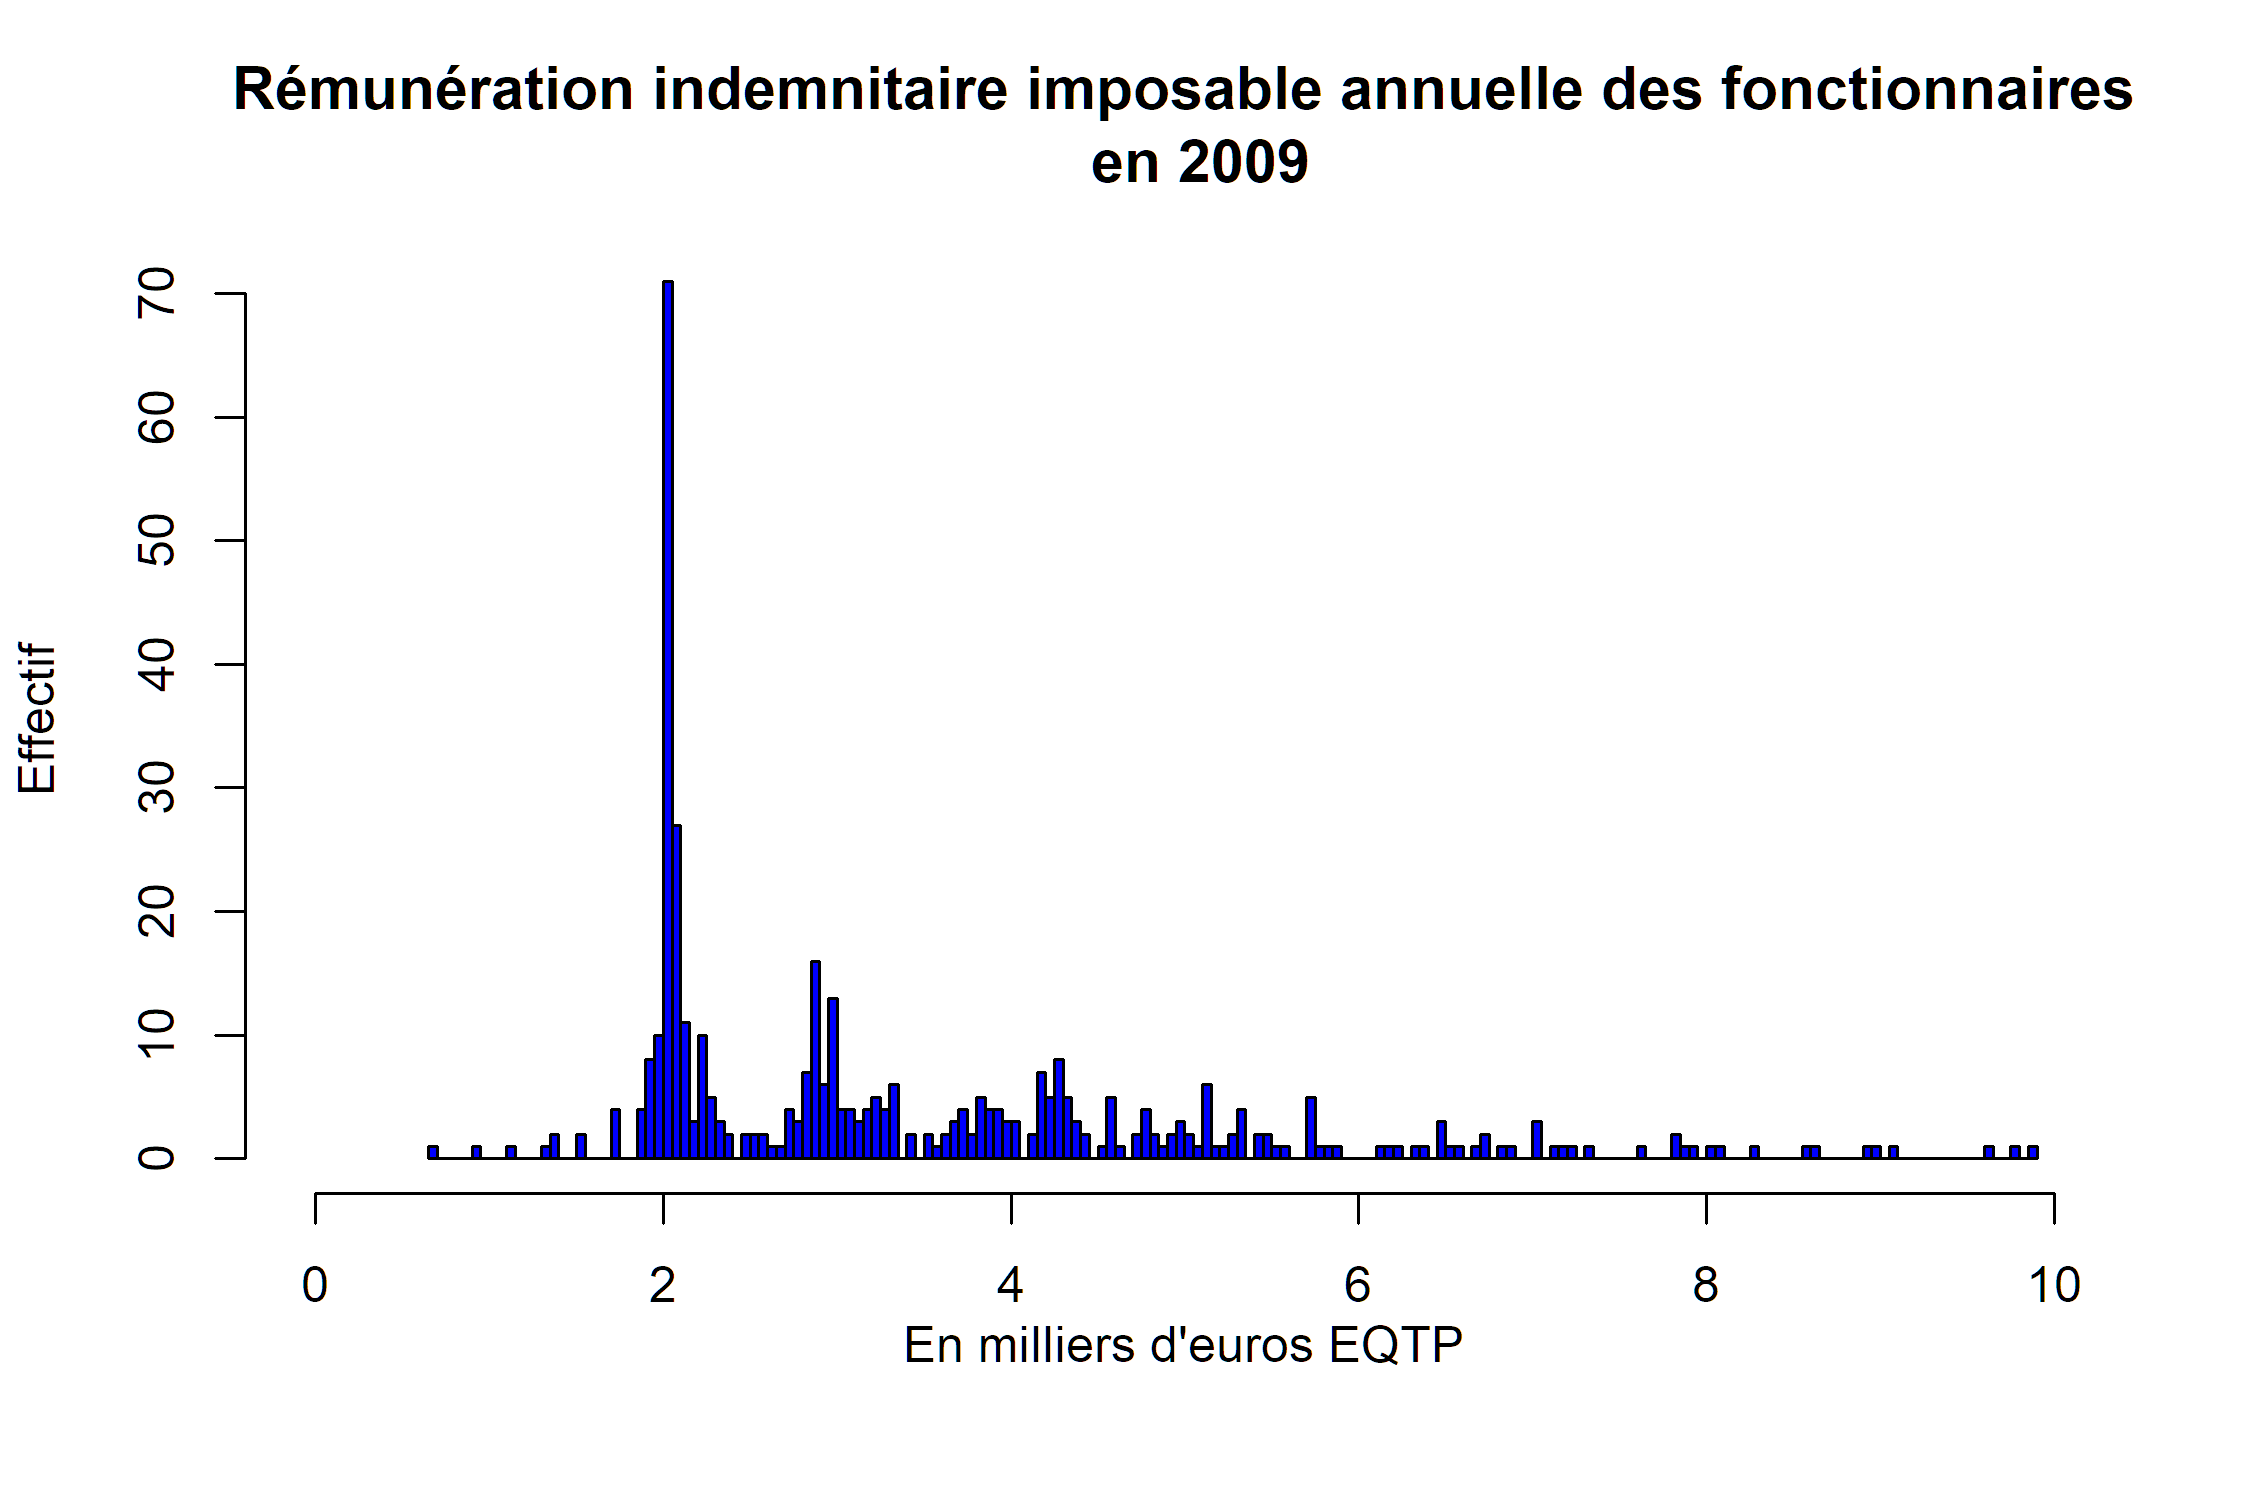
\includegraphics{altair_files/figure-latex/unnamed-chunk-43-3.png}

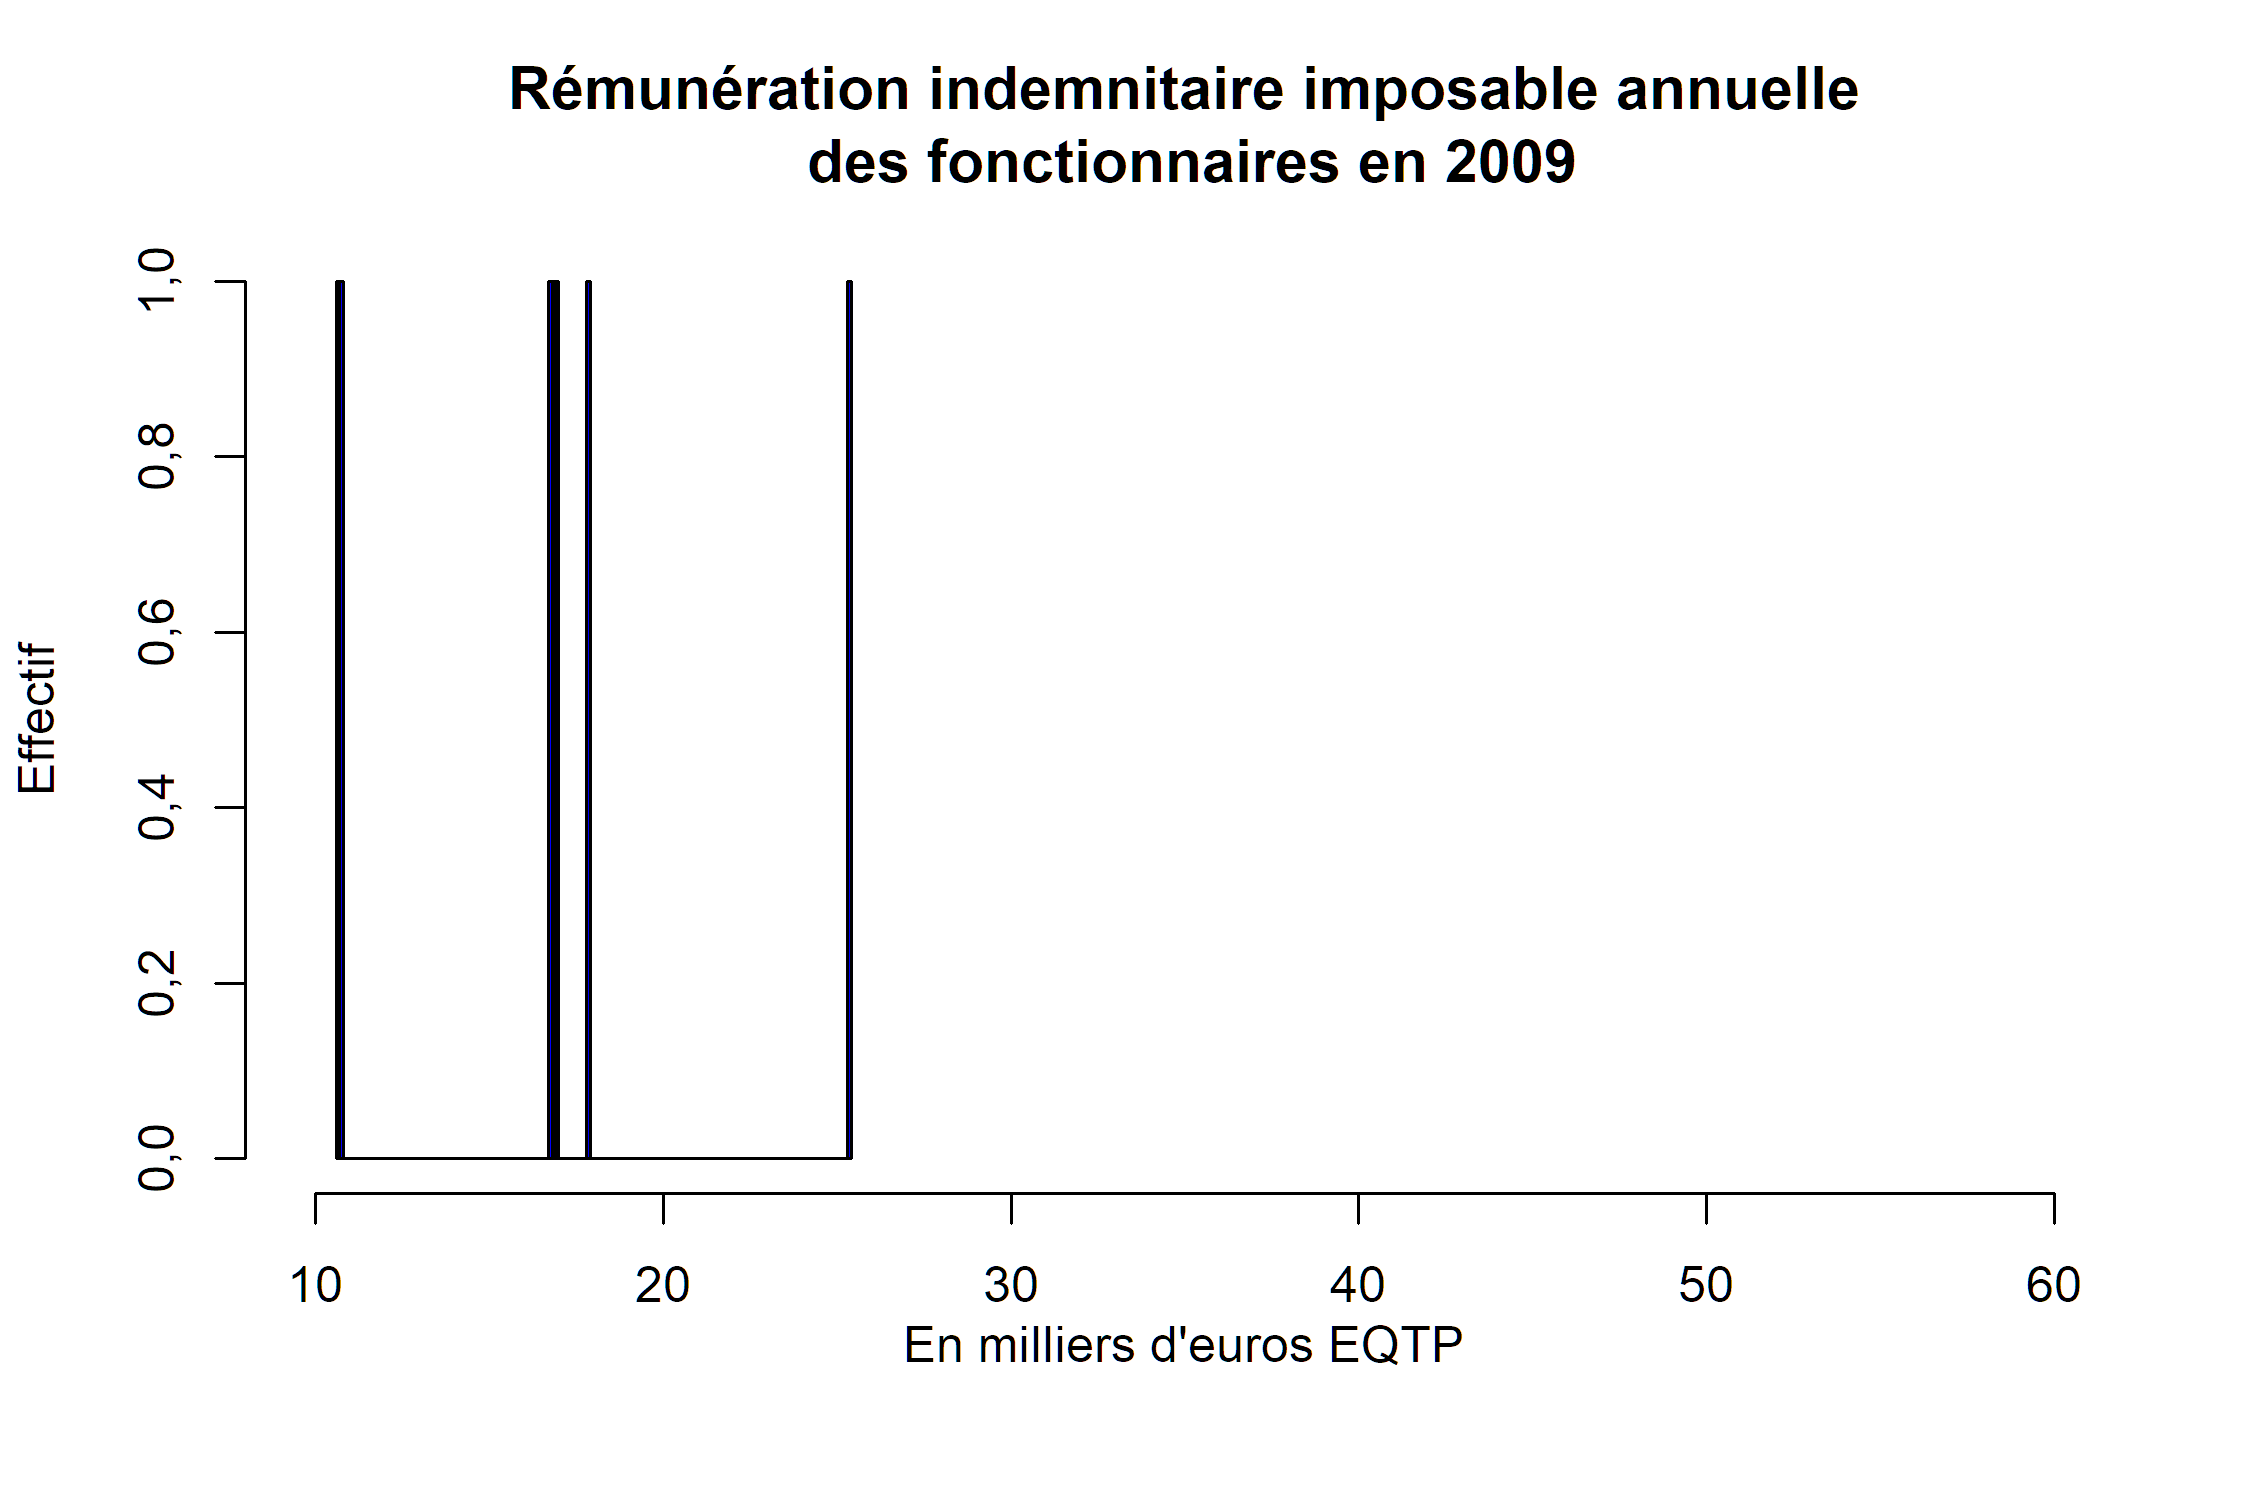
\includegraphics{altair_files/figure-latex/unnamed-chunk-43-4.png}

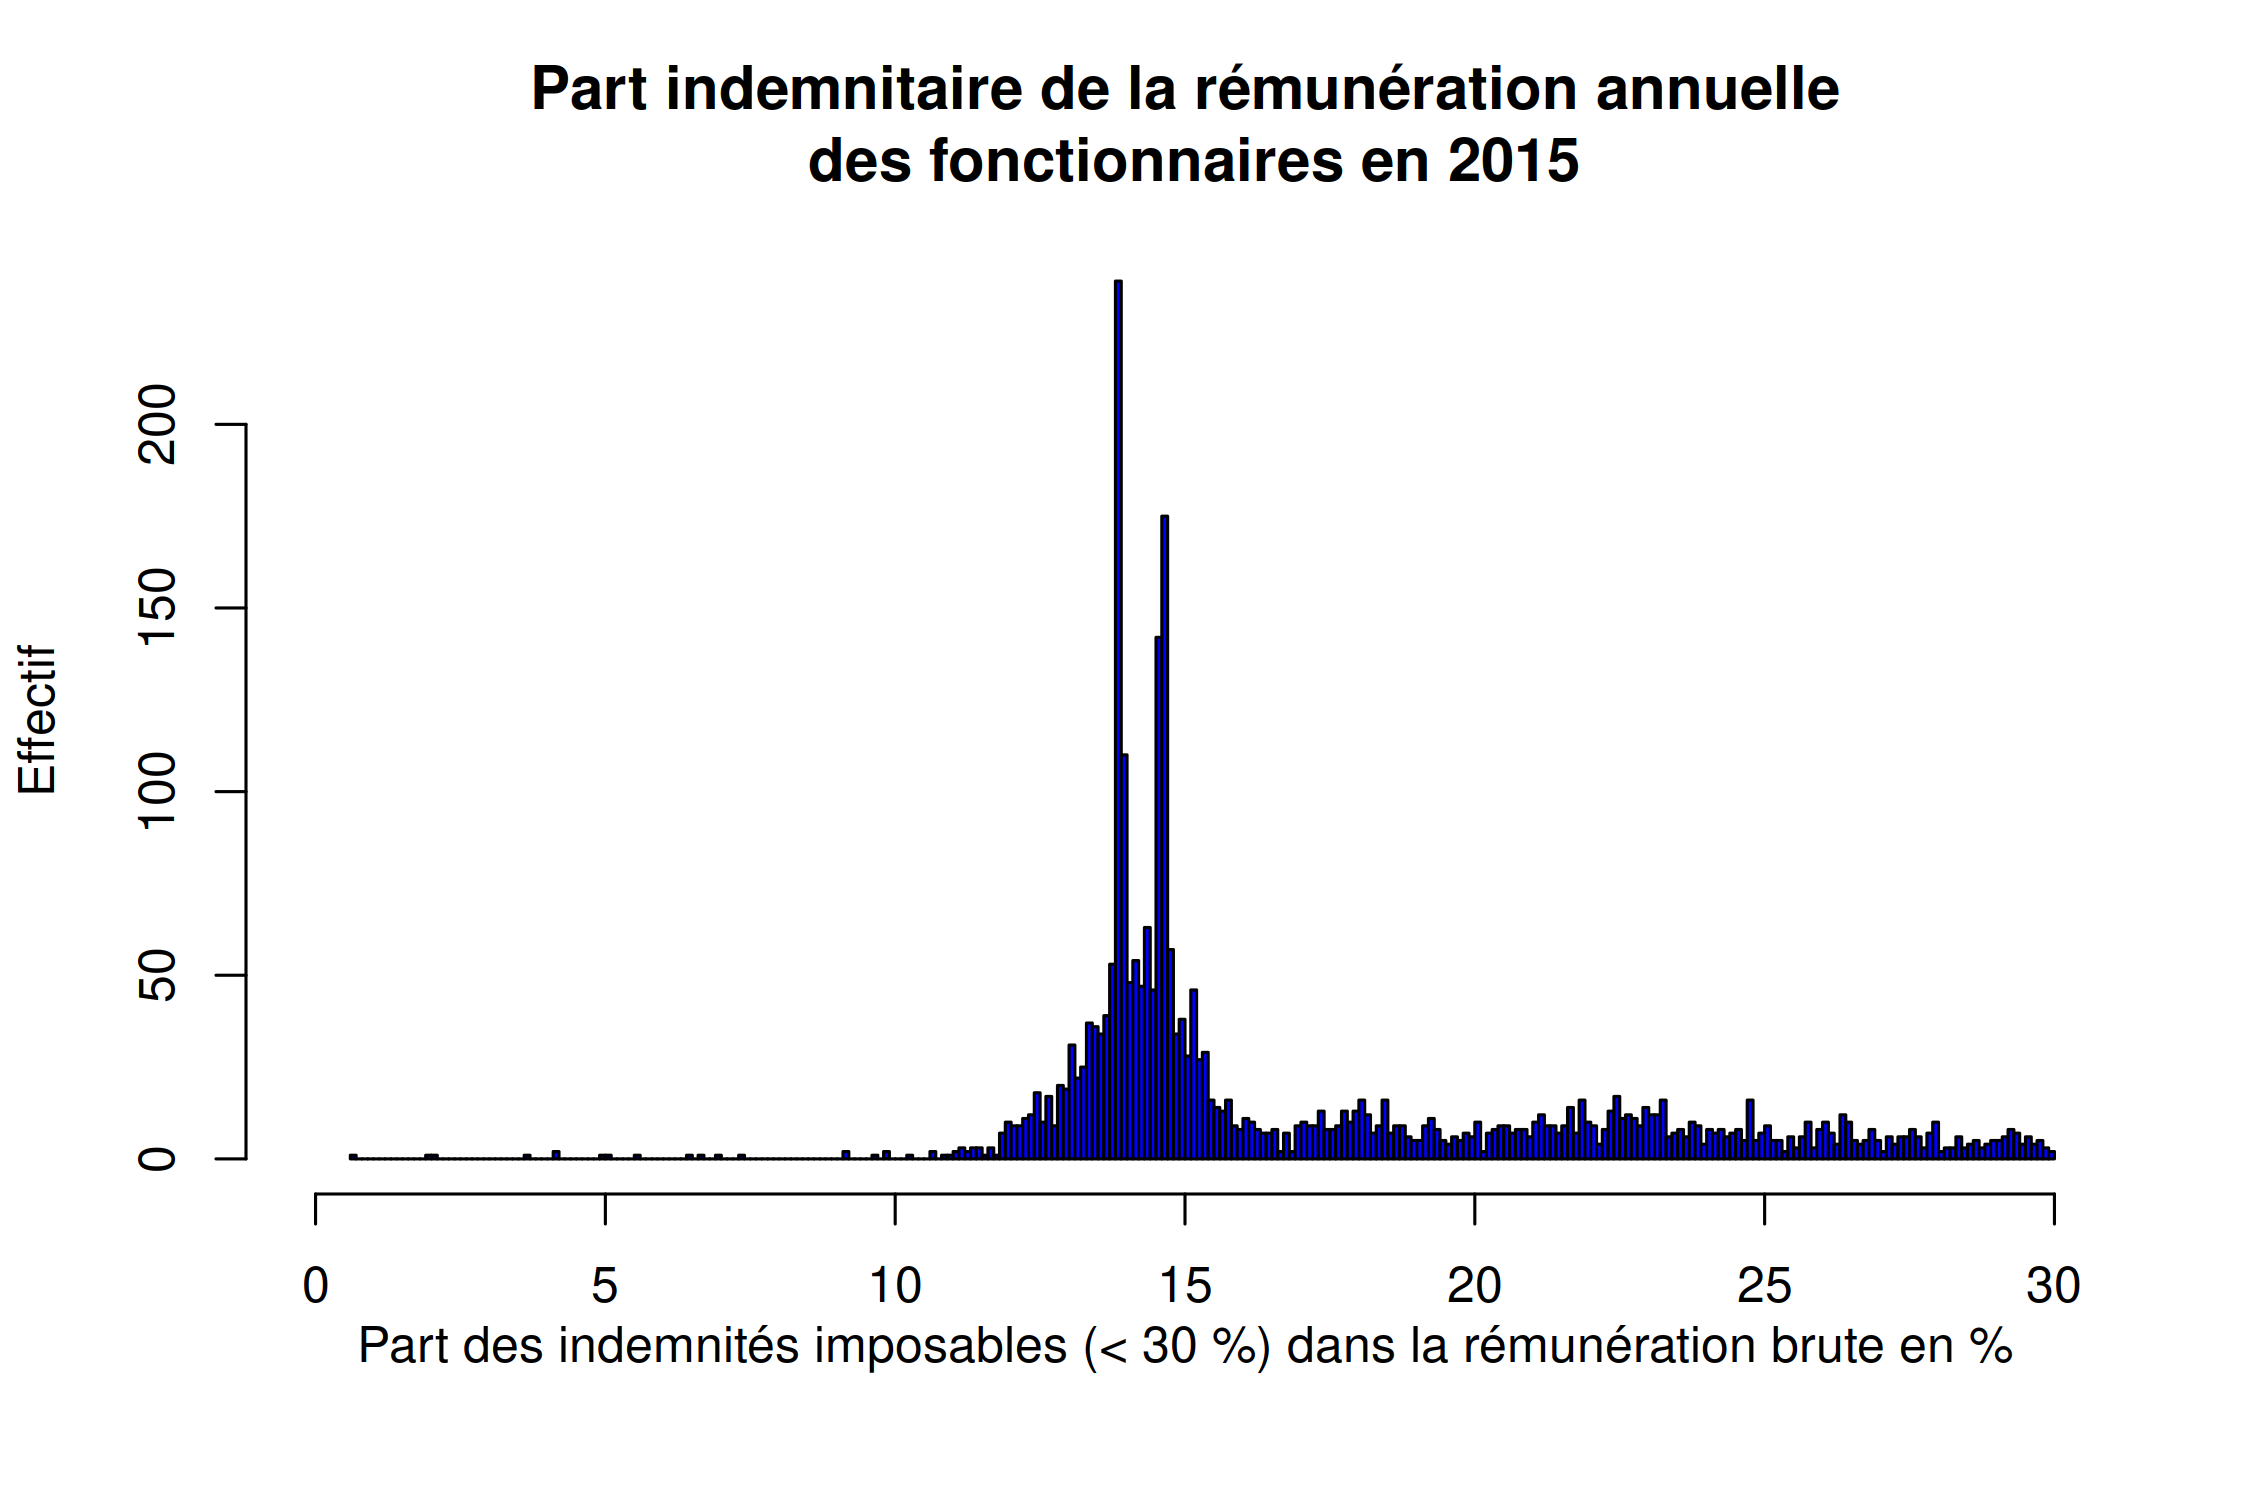
\includegraphics{altair_files/figure-latex/unnamed-chunk-43-5.png}

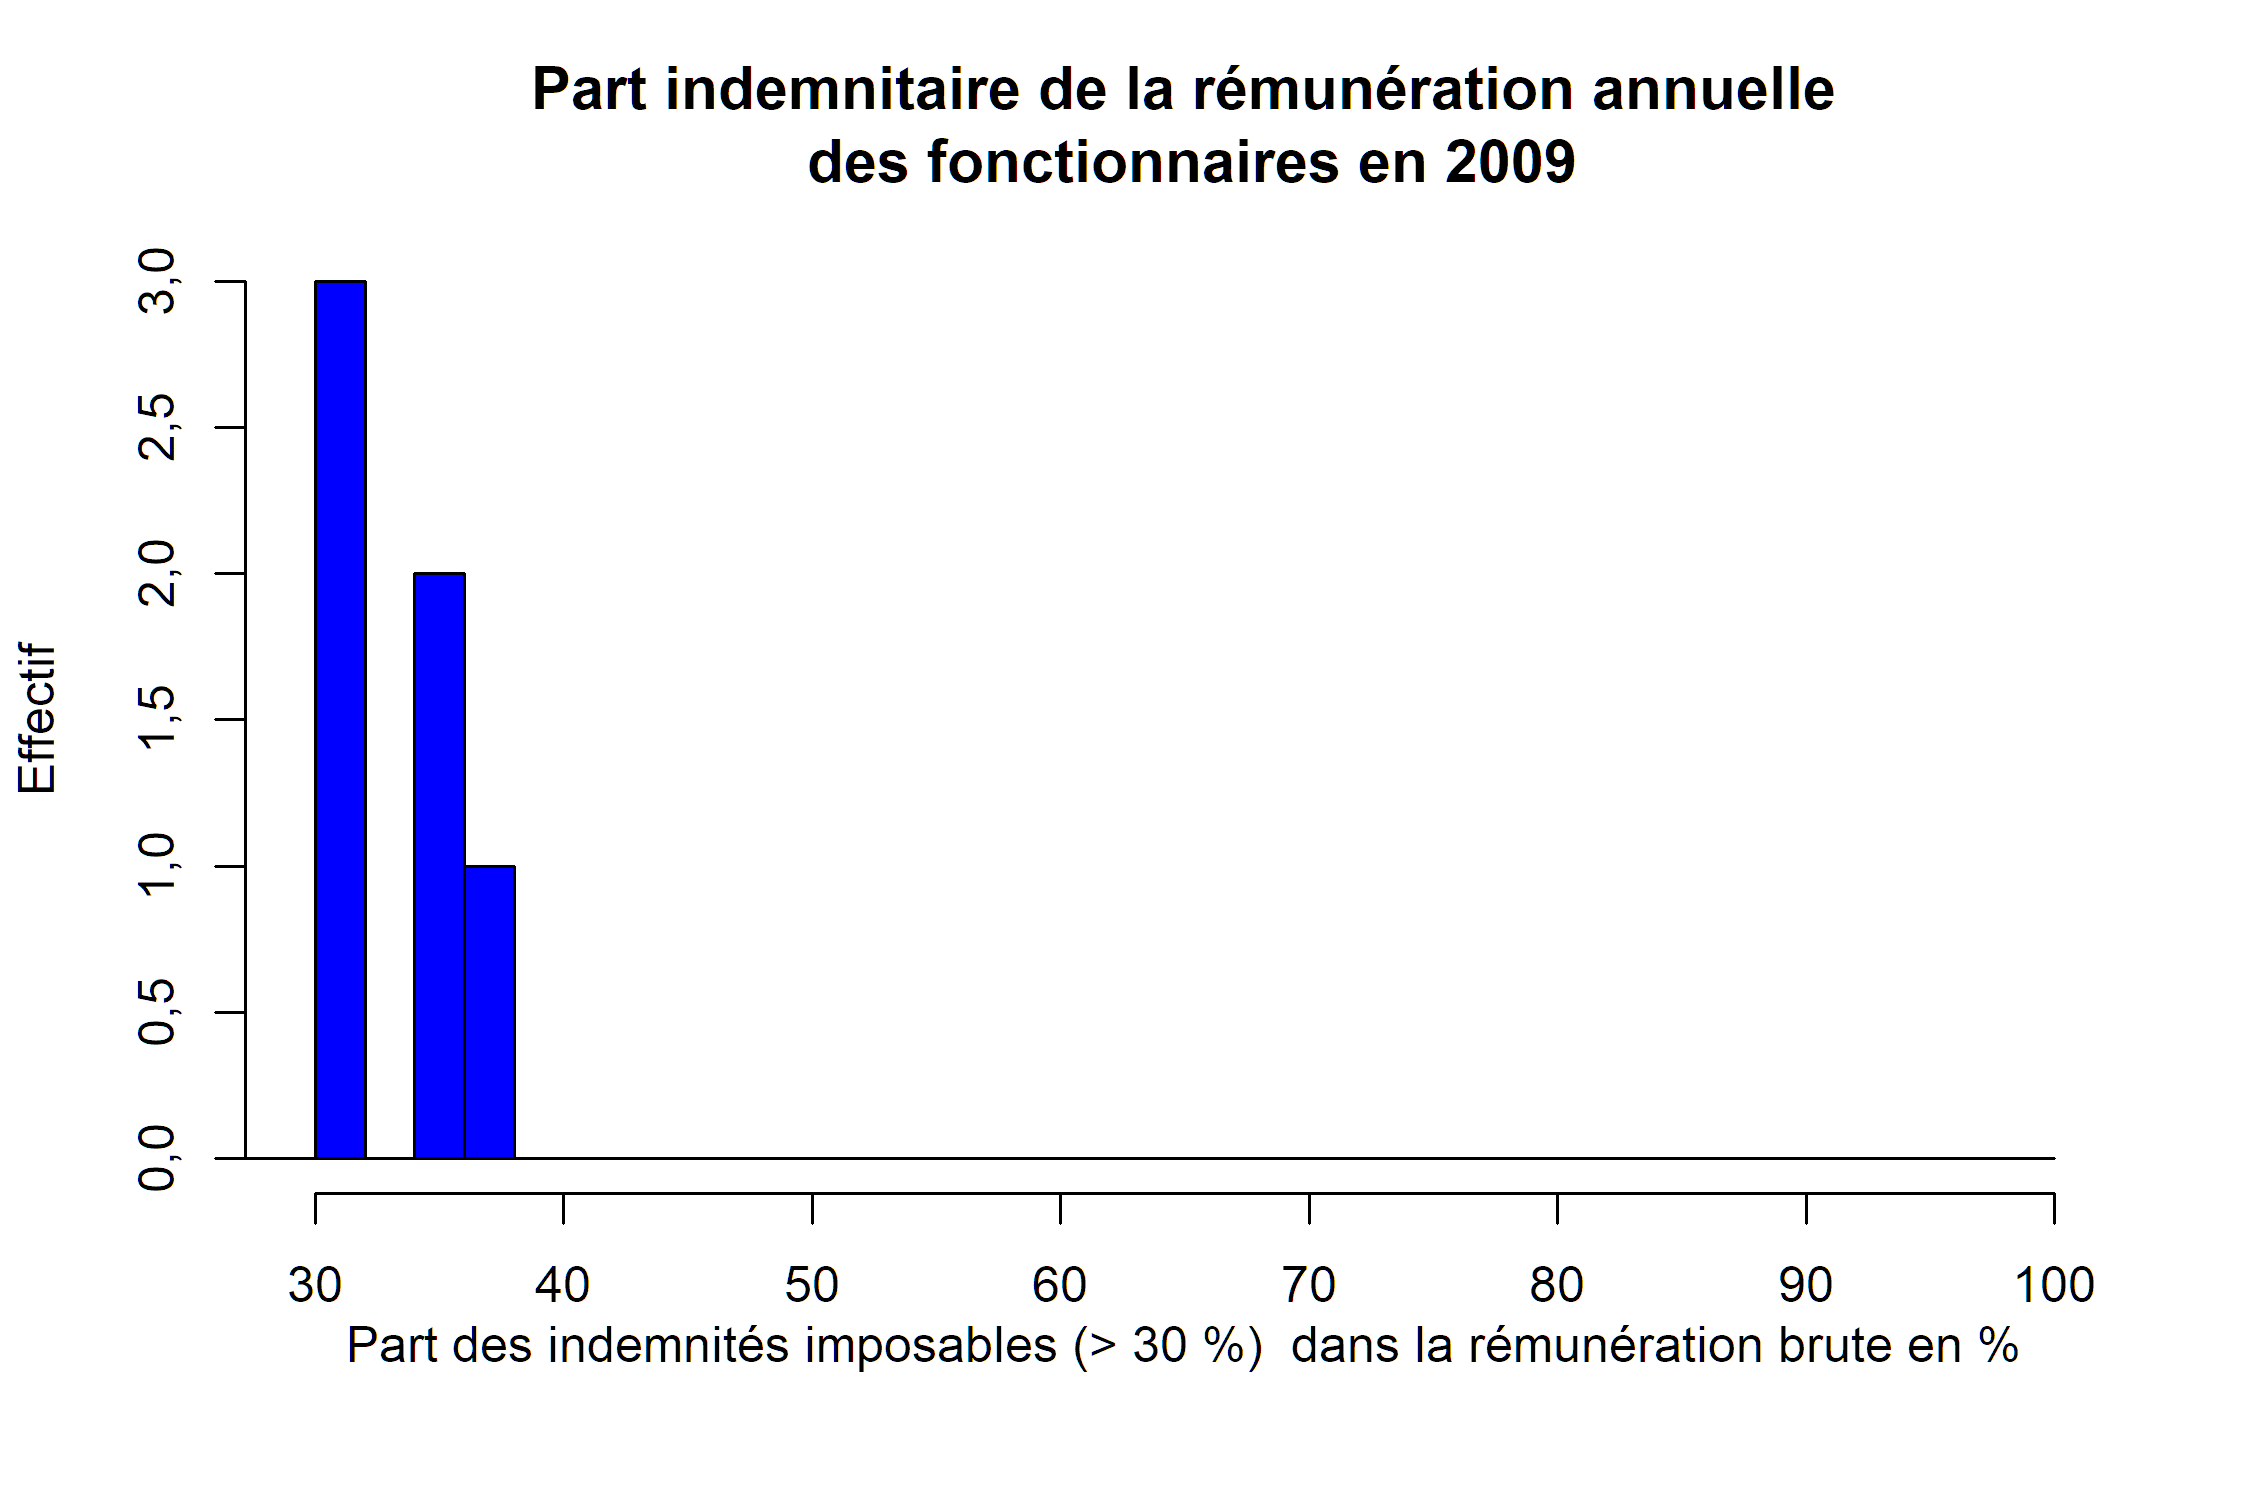
\includegraphics{altair_files/figure-latex/unnamed-chunk-43-6.png}

\textbf{Nota :}\\
\emph{Cet histogramme décrit l'évolution de la rémunération moyenne des
personnes en place (RMPP), définies comme présentes deux annees entières
consécutives avec la même quotité}\\
\emph{L'évolution de la RMPP permet d'étudier le glissement
vieillesse-technicité ``positif'', à effectifs constants sur deux
années}

\textbf{Effectif : 433 }

\textbf{Tests de cohérence}

Somme des rémunérations brutes versées aux personnels titulaires et
stagiaires :

~\emph{Tableau 2.2.1}

\begin{longtable}[]{@{}ll@{}}
\toprule
Agrégats & k€\tabularnewline
\midrule
\endhead
Brut annuel (bulletins) & 9 264 307,7\tabularnewline
Brut annuel (lignes) : & 9 263 639,5\tabularnewline
~dont ~~primes : & 1 419 599,3\tabularnewline
~dont ~autres rémunérations : &\tabularnewline
Part de primes en \% & 15,3\tabularnewline
\bottomrule
\end{longtable}

\textbf{Définitions :}

\emph{Brut annuel (bulletins)} : somme du champ \emph{Brut}\\
\emph{Brut annuel (lignes)} : somme du champ \emph{Montant} des lignes
de paye, dont :\\
\emph{Primes} : indemnités sauf remboursements, certaines IJSS,
Supplément familial de traitement et Indemnité de résidence\\
\emph{Autres rémunérations} : acomptes, retenues sur brut, rémunérations
diverses, rappels

\textbf{Tests de cohérence}

Somme des rémunérations brutes versées aux personnels (fonctionnaires) :

~\emph{Tableau 2.2.2}

\begin{longtable}[]{@{}ll@{}}
\toprule
Agrégats & k€\tabularnewline
\midrule
\endhead
Bulletins de paie & 9 264 307,7\tabularnewline
Lignes de paie & 9 263 639,5\tabularnewline
Difference & 668,2\tabularnewline
\bottomrule
\end{longtable}

A comparer aux soldes des comptes 6411, 6419 et 648 du compte de
gestion.

\textbf{Formation et distribution du salaire brut moyen par tête (SMPT)
en EQTP pour l'annee 2009 }

~\emph{Tableau 2.2.3}

\begin{longtable}[]{@{}rrrrrr@{}}
\toprule
\begin{minipage}[b]{0.14\columnwidth}\raggedleft
Statistique\strut
\end{minipage} & \begin{minipage}[b]{0.23\columnwidth}\raggedleft
Traitement indiciaire\strut
\end{minipage} & \begin{minipage}[b]{0.07\columnwidth}\raggedleft
Primes\strut
\end{minipage} & \begin{minipage}[b]{0.22\columnwidth}\raggedleft
Autres rémunérations\strut
\end{minipage} & \begin{minipage}[b]{0.08\columnwidth}\raggedleft
Quotité\strut
\end{minipage} & \begin{minipage}[b]{0.09\columnwidth}\raggedleft
Effectif\strut
\end{minipage}\tabularnewline
\midrule
\endhead
\begin{minipage}[t]{0.14\columnwidth}\raggedleft
Minimum\strut
\end{minipage} & \begin{minipage}[t]{0.23\columnwidth}\raggedleft
6 727\strut
\end{minipage} & \begin{minipage}[t]{0.07\columnwidth}\raggedleft
913\strut
\end{minipage} & \begin{minipage}[t]{0.22\columnwidth}\raggedleft
0\strut
\end{minipage} & \begin{minipage}[t]{0.08\columnwidth}\raggedleft
0,4\strut
\end{minipage} & \begin{minipage}[t]{0.09\columnwidth}\raggedleft
\strut
\end{minipage}\tabularnewline
\begin{minipage}[t]{0.14\columnwidth}\raggedleft
1er quartile\strut
\end{minipage} & \begin{minipage}[t]{0.23\columnwidth}\raggedleft
16 233\strut
\end{minipage} & \begin{minipage}[t]{0.07\columnwidth}\raggedleft
2 019\strut
\end{minipage} & \begin{minipage}[t]{0.22\columnwidth}\raggedleft
0\strut
\end{minipage} & \begin{minipage}[t]{0.08\columnwidth}\raggedleft
1\strut
\end{minipage} & \begin{minipage}[t]{0.09\columnwidth}\raggedleft
\strut
\end{minipage}\tabularnewline
\begin{minipage}[t]{0.14\columnwidth}\raggedleft
Médiane\strut
\end{minipage} & \begin{minipage}[t]{0.23\columnwidth}\raggedleft
17 567\strut
\end{minipage} & \begin{minipage}[t]{0.07\columnwidth}\raggedleft
2 884\strut
\end{minipage} & \begin{minipage}[t]{0.22\columnwidth}\raggedleft
0\strut
\end{minipage} & \begin{minipage}[t]{0.08\columnwidth}\raggedleft
1\strut
\end{minipage} & \begin{minipage}[t]{0.09\columnwidth}\raggedleft
\strut
\end{minipage}\tabularnewline
\begin{minipage}[t]{0.14\columnwidth}\raggedleft
Moyenne\strut
\end{minipage} & \begin{minipage}[t]{0.23\columnwidth}\raggedleft
19 203\strut
\end{minipage} & \begin{minipage}[t]{0.07\columnwidth}\raggedleft
3 511\strut
\end{minipage} & \begin{minipage}[t]{0.22\columnwidth}\raggedleft
0\strut
\end{minipage} & \begin{minipage}[t]{0.08\columnwidth}\raggedleft
0,96\strut
\end{minipage} & \begin{minipage}[t]{0.09\columnwidth}\raggedleft
411\strut
\end{minipage}\tabularnewline
\begin{minipage}[t]{0.14\columnwidth}\raggedleft
3ème quartile\strut
\end{minipage} & \begin{minipage}[t]{0.23\columnwidth}\raggedleft
20 855\strut
\end{minipage} & \begin{minipage}[t]{0.07\columnwidth}\raggedleft
4 215\strut
\end{minipage} & \begin{minipage}[t]{0.22\columnwidth}\raggedleft
0\strut
\end{minipage} & \begin{minipage}[t]{0.08\columnwidth}\raggedleft
1\strut
\end{minipage} & \begin{minipage}[t]{0.09\columnwidth}\raggedleft
\strut
\end{minipage}\tabularnewline
\begin{minipage}[t]{0.14\columnwidth}\raggedleft
Maximum\strut
\end{minipage} & \begin{minipage}[t]{0.23\columnwidth}\raggedleft
52 990\strut
\end{minipage} & \begin{minipage}[t]{0.07\columnwidth}\raggedleft
25 332\strut
\end{minipage} & \begin{minipage}[t]{0.22\columnwidth}\raggedleft
0\strut
\end{minipage} & \begin{minipage}[t]{0.08\columnwidth}\raggedleft
1\strut
\end{minipage} & \begin{minipage}[t]{0.09\columnwidth}\raggedleft
\strut
\end{minipage}\tabularnewline
\bottomrule
\end{longtable}

~\emph{Tableau 2.2.4}

\begin{longtable}[]{@{}rrrrrrr@{}}
\toprule
\begin{minipage}[b]{0.11\columnwidth}\raggedleft
Statistique\strut
\end{minipage} & \begin{minipage}[b]{0.20\columnwidth}\raggedleft
Total lignes hors rappels\strut
\end{minipage} & \begin{minipage}[b]{0.09\columnwidth}\raggedleft
Total brut\strut
\end{minipage} & \begin{minipage}[b]{0.14\columnwidth}\raggedleft
SMPT brut en EQTP\strut
\end{minipage} & \begin{minipage}[b]{0.14\columnwidth}\raggedleft
Part indemnitaire\strut
\end{minipage} & \begin{minipage}[b]{0.06\columnwidth}\raggedleft
Quotité\strut
\end{minipage} & \begin{minipage}[b]{0.07\columnwidth}\raggedleft
Effectif\strut
\end{minipage}\tabularnewline
\midrule
\endhead
\begin{minipage}[t]{0.11\columnwidth}\raggedleft
Minimum\strut
\end{minipage} & \begin{minipage}[t]{0.20\columnwidth}\raggedleft
8 139\strut
\end{minipage} & \begin{minipage}[t]{0.09\columnwidth}\raggedleft
8 139\strut
\end{minipage} & \begin{minipage}[t]{0.14\columnwidth}\raggedleft
9 585\strut
\end{minipage} & \begin{minipage}[t]{0.14\columnwidth}\raggedleft
5,1\strut
\end{minipage} & \begin{minipage}[t]{0.06\columnwidth}\raggedleft
0,4\strut
\end{minipage} & \begin{minipage}[t]{0.07\columnwidth}\raggedleft
\strut
\end{minipage}\tabularnewline
\begin{minipage}[t]{0.11\columnwidth}\raggedleft
1er quartile\strut
\end{minipage} & \begin{minipage}[t]{0.20\columnwidth}\raggedleft
18 923\strut
\end{minipage} & \begin{minipage}[t]{0.09\columnwidth}\raggedleft
19 014\strut
\end{minipage} & \begin{minipage}[t]{0.14\columnwidth}\raggedleft
19 087\strut
\end{minipage} & \begin{minipage}[t]{0.14\columnwidth}\raggedleft
11\strut
\end{minipage} & \begin{minipage}[t]{0.06\columnwidth}\raggedleft
1\strut
\end{minipage} & \begin{minipage}[t]{0.07\columnwidth}\raggedleft
\strut
\end{minipage}\tabularnewline
\begin{minipage}[t]{0.11\columnwidth}\raggedleft
Médiane\strut
\end{minipage} & \begin{minipage}[t]{0.20\columnwidth}\raggedleft
21 005\strut
\end{minipage} & \begin{minipage}[t]{0.09\columnwidth}\raggedleft
20 993\strut
\end{minipage} & \begin{minipage}[t]{0.14\columnwidth}\raggedleft
21 178\strut
\end{minipage} & \begin{minipage}[t]{0.14\columnwidth}\raggedleft
13\strut
\end{minipage} & \begin{minipage}[t]{0.06\columnwidth}\raggedleft
1\strut
\end{minipage} & \begin{minipage}[t]{0.07\columnwidth}\raggedleft
\strut
\end{minipage}\tabularnewline
\begin{minipage}[t]{0.11\columnwidth}\raggedleft
Moyenne\strut
\end{minipage} & \begin{minipage}[t]{0.20\columnwidth}\raggedleft
22 913\strut
\end{minipage} & \begin{minipage}[t]{0.09\columnwidth}\raggedleft
22 922\strut
\end{minipage} & \begin{minipage}[t]{0.14\columnwidth}\raggedleft
23 100\strut
\end{minipage} & \begin{minipage}[t]{0.14\columnwidth}\raggedleft
15\strut
\end{minipage} & \begin{minipage}[t]{0.06\columnwidth}\raggedleft
0,96\strut
\end{minipage} & \begin{minipage}[t]{0.07\columnwidth}\raggedleft
411\strut
\end{minipage}\tabularnewline
\begin{minipage}[t]{0.11\columnwidth}\raggedleft
3ème quartile\strut
\end{minipage} & \begin{minipage}[t]{0.20\columnwidth}\raggedleft
24 995\strut
\end{minipage} & \begin{minipage}[t]{0.09\columnwidth}\raggedleft
24 945\strut
\end{minipage} & \begin{minipage}[t]{0.14\columnwidth}\raggedleft
25 073\strut
\end{minipage} & \begin{minipage}[t]{0.14\columnwidth}\raggedleft
17\strut
\end{minipage} & \begin{minipage}[t]{0.06\columnwidth}\raggedleft
1\strut
\end{minipage} & \begin{minipage}[t]{0.07\columnwidth}\raggedleft
\strut
\end{minipage}\tabularnewline
\begin{minipage}[t]{0.11\columnwidth}\raggedleft
Maximum\strut
\end{minipage} & \begin{minipage}[t]{0.20\columnwidth}\raggedleft
70 613\strut
\end{minipage} & \begin{minipage}[t]{0.09\columnwidth}\raggedleft
70 580\strut
\end{minipage} & \begin{minipage}[t]{0.14\columnwidth}\raggedleft
70 580\strut
\end{minipage} & \begin{minipage}[t]{0.14\columnwidth}\raggedleft
37\strut
\end{minipage} & \begin{minipage}[t]{0.06\columnwidth}\raggedleft
1\strut
\end{minipage} & \begin{minipage}[t]{0.07\columnwidth}\raggedleft
\strut
\end{minipage}\tabularnewline
\bottomrule
\end{longtable}

\emph{Hors vacataires identifiés, assistantes maternelles, élus locaux
et pour les postes actifs non annexes}

\textbf{Categorie A}

~\emph{Tableau 2.2.5}

\begin{longtable}[]{@{}rrrrr@{}}
\toprule
Statistique & Traitement indiciaire & Primes & Autres rémunérations &
Quotité\tabularnewline
\midrule
\endhead
Minimum & 23 712 & 4 681 & 0 & 0,67\tabularnewline
1er quartile & 30 649 & 6 700 & 0 & 1\tabularnewline
Médiane & 35 877 & 8 056 & 0 & 1\tabularnewline
Moyenne & 36 281 & 10 177 & 0 & 0,98\tabularnewline
3ème quartile & 43 509 & 10 698 & 0 & 1\tabularnewline
Maximum & 52 990 & 25 332 & 0 & 1\tabularnewline
\bottomrule
\end{longtable}

~\emph{Tableau 2.2.6}

\begin{longtable}[]{@{}rrrrr@{}}
\toprule
\begin{minipage}[b]{0.14\columnwidth}\raggedleft
Statistique\strut
\end{minipage} & \begin{minipage}[b]{0.20\columnwidth}\raggedleft
Total rémunérations\strut
\end{minipage} & \begin{minipage}[b]{0.25\columnwidth}\raggedleft
Total rémunérations EQTP\strut
\end{minipage} & \begin{minipage}[b]{0.18\columnwidth}\raggedleft
Part indemnitaire\strut
\end{minipage} & \begin{minipage}[b]{0.08\columnwidth}\raggedleft
Quotité\strut
\end{minipage}\tabularnewline
\midrule
\endhead
\begin{minipage}[t]{0.14\columnwidth}\raggedleft
Minimum\strut
\end{minipage} & \begin{minipage}[t]{0.20\columnwidth}\raggedleft
29 430\strut
\end{minipage} & \begin{minipage}[t]{0.25\columnwidth}\raggedleft
29 430\strut
\end{minipage} & \begin{minipage}[t]{0.18\columnwidth}\raggedleft
14\strut
\end{minipage} & \begin{minipage}[t]{0.08\columnwidth}\raggedleft
0,67\strut
\end{minipage}\tabularnewline
\begin{minipage}[t]{0.14\columnwidth}\raggedleft
1er quartile\strut
\end{minipage} & \begin{minipage}[t]{0.20\columnwidth}\raggedleft
38 406\strut
\end{minipage} & \begin{minipage}[t]{0.25\columnwidth}\raggedleft
39 056\strut
\end{minipage} & \begin{minipage}[t]{0.18\columnwidth}\raggedleft
17\strut
\end{minipage} & \begin{minipage}[t]{0.08\columnwidth}\raggedleft
1\strut
\end{minipage}\tabularnewline
\begin{minipage}[t]{0.14\columnwidth}\raggedleft
Médiane\strut
\end{minipage} & \begin{minipage}[t]{0.20\columnwidth}\raggedleft
42 616\strut
\end{minipage} & \begin{minipage}[t]{0.25\columnwidth}\raggedleft
46 221\strut
\end{minipage} & \begin{minipage}[t]{0.18\columnwidth}\raggedleft
19\strut
\end{minipage} & \begin{minipage}[t]{0.08\columnwidth}\raggedleft
1\strut
\end{minipage}\tabularnewline
\begin{minipage}[t]{0.14\columnwidth}\raggedleft
Moyenne\strut
\end{minipage} & \begin{minipage}[t]{0.20\columnwidth}\raggedleft
46 273\strut
\end{minipage} & \begin{minipage}[t]{0.25\columnwidth}\raggedleft
47 275\strut
\end{minipage} & \begin{minipage}[t]{0.18\columnwidth}\raggedleft
21\strut
\end{minipage} & \begin{minipage}[t]{0.08\columnwidth}\raggedleft
0,98\strut
\end{minipage}\tabularnewline
\begin{minipage}[t]{0.14\columnwidth}\raggedleft
3ème quartile\strut
\end{minipage} & \begin{minipage}[t]{0.20\columnwidth}\raggedleft
54 772\strut
\end{minipage} & \begin{minipage}[t]{0.25\columnwidth}\raggedleft
54 772\strut
\end{minipage} & \begin{minipage}[t]{0.18\columnwidth}\raggedleft
26\strut
\end{minipage} & \begin{minipage}[t]{0.08\columnwidth}\raggedleft
1\strut
\end{minipage}\tabularnewline
\begin{minipage}[t]{0.14\columnwidth}\raggedleft
Maximum\strut
\end{minipage} & \begin{minipage}[t]{0.20\columnwidth}\raggedleft
70 580\strut
\end{minipage} & \begin{minipage}[t]{0.25\columnwidth}\raggedleft
70 580\strut
\end{minipage} & \begin{minipage}[t]{0.18\columnwidth}\raggedleft
36\strut
\end{minipage} & \begin{minipage}[t]{0.08\columnwidth}\raggedleft
1\strut
\end{minipage}\tabularnewline
\bottomrule
\end{longtable}

\textbf{Effectif : 24 }

\textbf{Categorie B}

~\emph{Tableau 2.2.7}

\begin{longtable}[]{@{}rrrrr@{}}
\toprule
Statistique & Traitement indiciaire & Primes & Autres rémunérations &
Quotité\tabularnewline
\midrule
\endhead
Minimum & 15 174 & 3 650 & 0 & 0,7\tabularnewline
1er quartile & 19 856 & 4 336 & 0 & 1\tabularnewline
Médiane & 22 770 & 4 983 & 0 & 1\tabularnewline
Moyenne & 22 494 & 5 541 & 0 & 0,97\tabularnewline
3ème quartile & 25 060 & 6 782 & 0 & 1\tabularnewline
Maximum & 29 384 & 10 775 & 0 & 1\tabularnewline
\bottomrule
\end{longtable}

~\emph{Tableau 2.2.8}

\begin{longtable}[]{@{}rrrrr@{}}
\toprule
\begin{minipage}[b]{0.12\columnwidth}\raggedleft
Statistique\strut
\end{minipage} & \begin{minipage}[b]{0.17\columnwidth}\raggedleft
Total rémunérations\strut
\end{minipage} & \begin{minipage}[b]{0.21\columnwidth}\raggedleft
Total rémunérations EQTP\strut
\end{minipage} & \begin{minipage}[b]{0.31\columnwidth}\raggedleft
Part de la rémunération indemnitaire\strut
\end{minipage} & \begin{minipage}[b]{0.07\columnwidth}\raggedleft
Quotité\strut
\end{minipage}\tabularnewline
\midrule
\endhead
\begin{minipage}[t]{0.12\columnwidth}\raggedleft
Minimum\strut
\end{minipage} & \begin{minipage}[t]{0.17\columnwidth}\raggedleft
20 857\strut
\end{minipage} & \begin{minipage}[t]{0.21\columnwidth}\raggedleft
22 485\strut
\end{minipage} & \begin{minipage}[t]{0.31\columnwidth}\raggedleft
14\strut
\end{minipage} & \begin{minipage}[t]{0.07\columnwidth}\raggedleft
0,7\strut
\end{minipage}\tabularnewline
\begin{minipage}[t]{0.12\columnwidth}\raggedleft
1er quartile\strut
\end{minipage} & \begin{minipage}[t]{0.17\columnwidth}\raggedleft
24 665\strut
\end{minipage} & \begin{minipage}[t]{0.21\columnwidth}\raggedleft
25 045\strut
\end{minipage} & \begin{minipage}[t]{0.31\columnwidth}\raggedleft
16\strut
\end{minipage} & \begin{minipage}[t]{0.07\columnwidth}\raggedleft
1\strut
\end{minipage}\tabularnewline
\begin{minipage}[t]{0.12\columnwidth}\raggedleft
Médiane\strut
\end{minipage} & \begin{minipage}[t]{0.17\columnwidth}\raggedleft
27 569\strut
\end{minipage} & \begin{minipage}[t]{0.21\columnwidth}\raggedleft
27 711\strut
\end{minipage} & \begin{minipage}[t]{0.31\columnwidth}\raggedleft
19\strut
\end{minipage} & \begin{minipage}[t]{0.07\columnwidth}\raggedleft
1\strut
\end{minipage}\tabularnewline
\begin{minipage}[t]{0.12\columnwidth}\raggedleft
Moyenne\strut
\end{minipage} & \begin{minipage}[t]{0.17\columnwidth}\raggedleft
28 045\strut
\end{minipage} & \begin{minipage}[t]{0.21\columnwidth}\raggedleft
28 310\strut
\end{minipage} & \begin{minipage}[t]{0.31\columnwidth}\raggedleft
20\strut
\end{minipage} & \begin{minipage}[t]{0.07\columnwidth}\raggedleft
0,97\strut
\end{minipage}\tabularnewline
\begin{minipage}[t]{0.12\columnwidth}\raggedleft
3ème quartile\strut
\end{minipage} & \begin{minipage}[t]{0.17\columnwidth}\raggedleft
31 469\strut
\end{minipage} & \begin{minipage}[t]{0.21\columnwidth}\raggedleft
31 469\strut
\end{minipage} & \begin{minipage}[t]{0.31\columnwidth}\raggedleft
23\strut
\end{minipage} & \begin{minipage}[t]{0.07\columnwidth}\raggedleft
1\strut
\end{minipage}\tabularnewline
\begin{minipage}[t]{0.12\columnwidth}\raggedleft
Maximum\strut
\end{minipage} & \begin{minipage}[t]{0.17\columnwidth}\raggedleft
36 959\strut
\end{minipage} & \begin{minipage}[t]{0.21\columnwidth}\raggedleft
36 959\strut
\end{minipage} & \begin{minipage}[t]{0.31\columnwidth}\raggedleft
31\strut
\end{minipage} & \begin{minipage}[t]{0.07\columnwidth}\raggedleft
1\strut
\end{minipage}\tabularnewline
\bottomrule
\end{longtable}

\textbf{Effectif : 53 }

\textbf{Categorie C}

~\emph{Tableau 2.2.9}

\begin{longtable}[]{@{}rrrrr@{}}
\toprule
Statistique & Traitement indiciaire & Primes & Autres rémunérations &
Quotité\tabularnewline
\midrule
\endhead
Minimum & 6 727 & 913 & 0 & 0,4\tabularnewline
1er quartile & 16 149 & 2 018 & 0 & 1\tabularnewline
Médiane & 17 016 & 2 284 & 0 & 1\tabularnewline
Moyenne & 17 489 & 2 771 & 0 & 0,95\tabularnewline
3ème quartile & 19 259 & 3 278 & 0 & 1\tabularnewline
Maximum & 25 843 & 7 200 & 0 & 1\tabularnewline
\bottomrule
\end{longtable}

~\emph{Tableau 2.2.10}

\begin{longtable}[]{@{}rrrrr@{}}
\toprule
\begin{minipage}[b]{0.12\columnwidth}\raggedleft
Statistique\strut
\end{minipage} & \begin{minipage}[b]{0.17\columnwidth}\raggedleft
Total rémunérations\strut
\end{minipage} & \begin{minipage}[b]{0.21\columnwidth}\raggedleft
Total rémunérations EQTP\strut
\end{minipage} & \begin{minipage}[b]{0.31\columnwidth}\raggedleft
Part de la rémunération indemnitaire\strut
\end{minipage} & \begin{minipage}[b]{0.07\columnwidth}\raggedleft
Quotité\strut
\end{minipage}\tabularnewline
\midrule
\endhead
\begin{minipage}[t]{0.12\columnwidth}\raggedleft
Minimum\strut
\end{minipage} & \begin{minipage}[t]{0.17\columnwidth}\raggedleft
8 139\strut
\end{minipage} & \begin{minipage}[t]{0.21\columnwidth}\raggedleft
9 585\strut
\end{minipage} & \begin{minipage}[t]{0.31\columnwidth}\raggedleft
5,1\strut
\end{minipage} & \begin{minipage}[t]{0.07\columnwidth}\raggedleft
0,4\strut
\end{minipage}\tabularnewline
\begin{minipage}[t]{0.12\columnwidth}\raggedleft
1er quartile\strut
\end{minipage} & \begin{minipage}[t]{0.17\columnwidth}\raggedleft
18 540\strut
\end{minipage} & \begin{minipage}[t]{0.21\columnwidth}\raggedleft
18 657\strut
\end{minipage} & \begin{minipage}[t]{0.31\columnwidth}\raggedleft
10\strut
\end{minipage} & \begin{minipage}[t]{0.07\columnwidth}\raggedleft
1\strut
\end{minipage}\tabularnewline
\begin{minipage}[t]{0.12\columnwidth}\raggedleft
Médiane\strut
\end{minipage} & \begin{minipage}[t]{0.17\columnwidth}\raggedleft
19 989\strut
\end{minipage} & \begin{minipage}[t]{0.21\columnwidth}\raggedleft
20 046\strut
\end{minipage} & \begin{minipage}[t]{0.31\columnwidth}\raggedleft
12\strut
\end{minipage} & \begin{minipage}[t]{0.07\columnwidth}\raggedleft
1\strut
\end{minipage}\tabularnewline
\begin{minipage}[t]{0.12\columnwidth}\raggedleft
Moyenne\strut
\end{minipage} & \begin{minipage}[t]{0.17\columnwidth}\raggedleft
20 550\strut
\end{minipage} & \begin{minipage}[t]{0.21\columnwidth}\raggedleft
20 667\strut
\end{minipage} & \begin{minipage}[t]{0.31\columnwidth}\raggedleft
13\strut
\end{minipage} & \begin{minipage}[t]{0.07\columnwidth}\raggedleft
0,95\strut
\end{minipage}\tabularnewline
\begin{minipage}[t]{0.12\columnwidth}\raggedleft
3ème quartile\strut
\end{minipage} & \begin{minipage}[t]{0.17\columnwidth}\raggedleft
22 645\strut
\end{minipage} & \begin{minipage}[t]{0.21\columnwidth}\raggedleft
22 743\strut
\end{minipage} & \begin{minipage}[t]{0.31\columnwidth}\raggedleft
15\strut
\end{minipage} & \begin{minipage}[t]{0.07\columnwidth}\raggedleft
1\strut
\end{minipage}\tabularnewline
\begin{minipage}[t]{0.12\columnwidth}\raggedleft
Maximum\strut
\end{minipage} & \begin{minipage}[t]{0.17\columnwidth}\raggedleft
33 991\strut
\end{minipage} & \begin{minipage}[t]{0.21\columnwidth}\raggedleft
33 991\strut
\end{minipage} & \begin{minipage}[t]{0.31\columnwidth}\raggedleft
37\strut
\end{minipage} & \begin{minipage}[t]{0.07\columnwidth}\raggedleft
1\strut
\end{minipage}\tabularnewline
\bottomrule
\end{longtable}

\textbf{Effectif : 310 }

\hypertarget{contractuels-vacataires-et-stagiaires-inclus}{%
\subsection{2.3 Contractuels, vacataires et stagiaires
inclus}\label{contractuels-vacataires-et-stagiaires-inclus}}

\emph{Les assistantes maternelles et les vacataires sont ici inclus,
pour les postes non annexes}

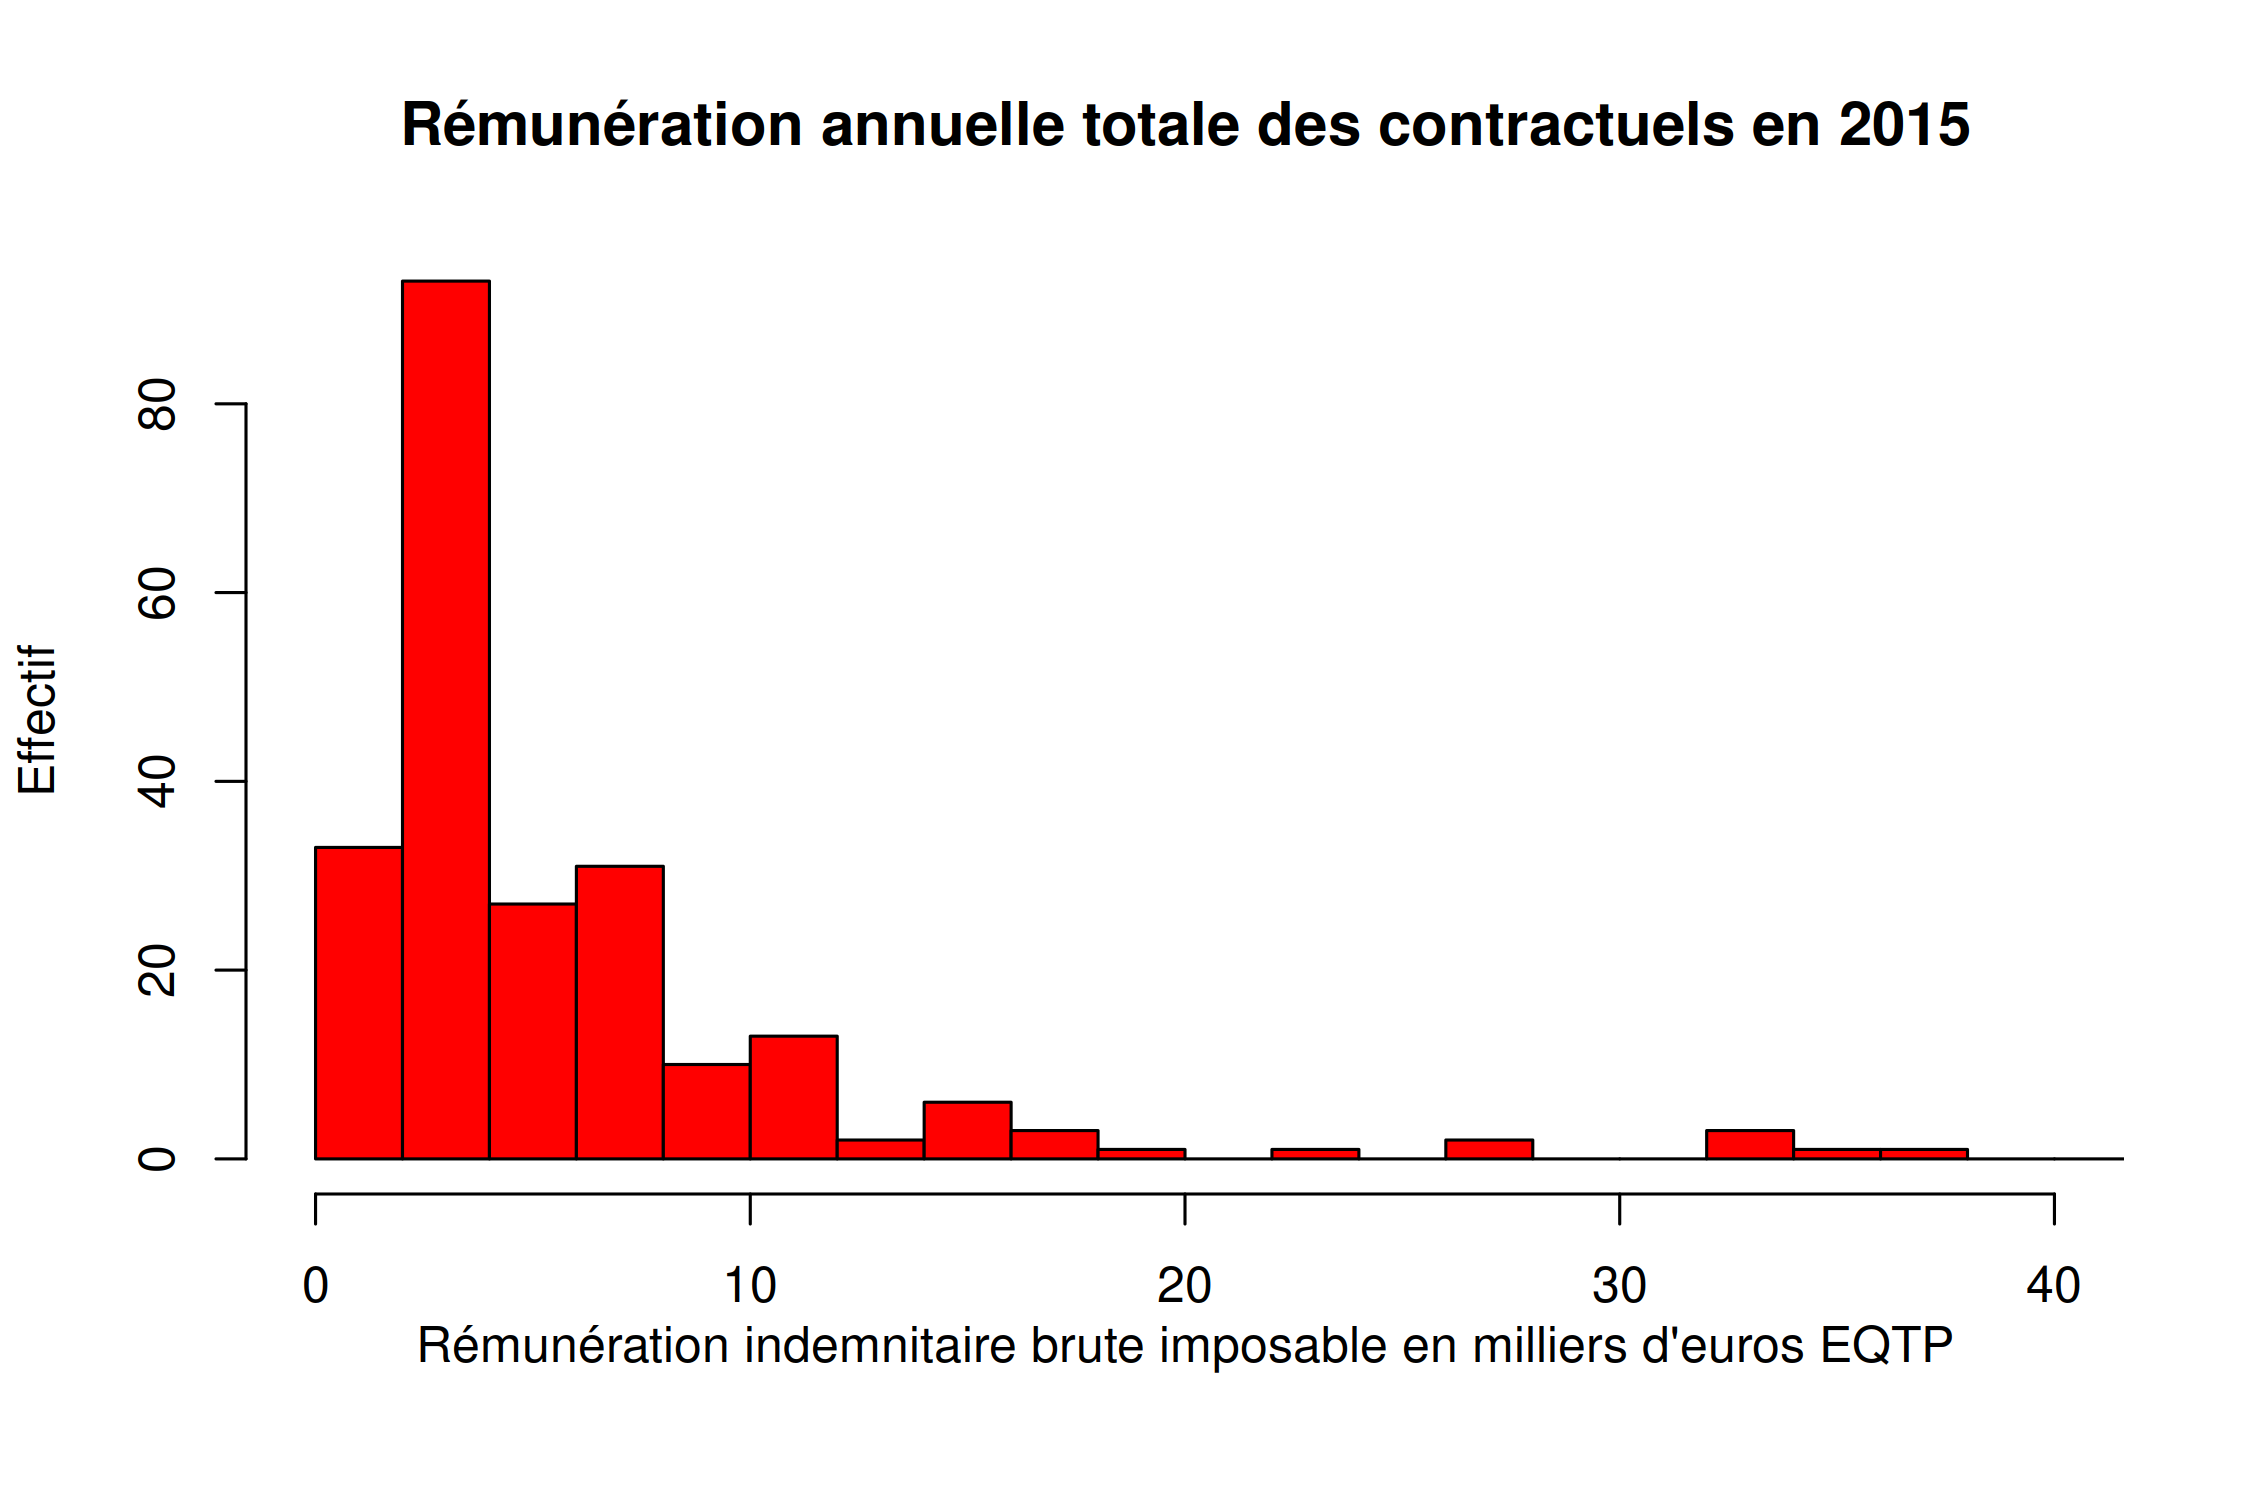
\includegraphics{altair_files/figure-latex/unnamed-chunk-61-1.png}

\textbf{Nota :} Ne sont retenues que les rémunérations supérieures à 1
000 k€. Les élus ne sont pas pris en compte.

\textbf{Formation et distribution du salaire brut moyen par tête (SMPT)
en EQTP pour l'année 2009 }

~\emph{Tableau 2.3.1}

\begin{longtable}[]{@{}rrrrr@{}}
\toprule
Statistique & Primes & Autres rémunérations & Quotité &
Effectif\tabularnewline
\midrule
\endhead
Minimum & -80 & 0 & 0,28 &\tabularnewline
1er quartile & 31 & 0 & 0,62 &\tabularnewline
Médiane & 800 & 0 & 0,89 &\tabularnewline
Moyenne & 1 426 & 0 & 0,79 & 65\tabularnewline
3ème quartile & 1 949 & 0 & 1 &\tabularnewline
Maximum & 6 358 & 0 & 1 &\tabularnewline
\bottomrule
\end{longtable}

~\emph{Tableau 2.3.2}

\begin{longtable}[]{@{}rrrrr@{}}
\toprule
Statistique & Total rémunérations & Total rémunérations EQTP & Quotité &
Effectif\tabularnewline
\midrule
\endhead
Minimum & 4 912 & 7 968 & 0,28 &\tabularnewline
1er quartile & 10 776 & 14 089 & 0,62 &\tabularnewline
Médiane & 16 453 & 16 576 & 0,89 &\tabularnewline
Moyenne & 17 244 & 18 637 & 0,79 & 65\tabularnewline
3ème quartile & 20 254 & 20 692 & 1 &\tabularnewline
Maximum & 52 654 & 52 654 & 1 &\tabularnewline
\bottomrule
\end{longtable}

\href{Bases/Remunerations/Analyse.remunerations.csv}{Lien vers la base
des rémunérations}

\newpage

\hypertarget{remunerations-brutes-analyse-pour-le-dernier-exercice}{%
\section{3. Rémunérations brutes : analyse pour le dernier
exercice}\label{remunerations-brutes-analyse-pour-le-dernier-exercice}}

\textbf{Exercice : 2013 }

\hypertarget{masse-salariale-brute-de-lensemble-des-agents-1}{%
\subsection{3.1 Masse salariale brute de l'ensemble des
agents}\label{masse-salariale-brute-de-lensemble-des-agents-1}}

\textbf{Cumuls des rémunérations brutes pour l'exercice 2013 }

\emph{Personnels (hors élus)}

~\emph{Tableau 3.1.1}

\begin{longtable}[]{@{}ll@{}}
\toprule
Agrégats & k€\tabularnewline
\midrule
\endhead
Brut annuel (bulletins) & 10 785 759,3\tabularnewline
Brut annuel (lignes) : & 10 804 648,0\tabularnewline
~dont ~Primes : & 1 780 299,9\tabularnewline
~dont ~Autres rémunérations &\tabularnewline
Part de primes en \% & 16,5\tabularnewline
\bottomrule
\end{longtable}

\textbf{Définitions :}

\emph{Brut annuel (bulletins)} : somme du champ \emph{Brut}\\
\emph{Brut annuel (lignes)} : somme du champ \emph{Montant} des lignes
de paye, dont :\\
\emph{Primes} : indemnités sauf remboursements, certaines IJSS,
indemnités d'élu le cas échéant, Supplément familial de traitement et
Indemnité de résidence\\
\emph{Autres rémunérations} : acomptes, retenues sur brut, rémunérations
diverses, rappels

\textbf{Tests de cohérence}

Somme des rémunérations brutes versées aux personnels (non élus) :

~\emph{Tableau 3.1.2}

\begin{longtable}[]{@{}ll@{}}
\toprule
Agrégats & k€\tabularnewline
\midrule
\endhead
Bulletins de paie & 10 785 759,3\tabularnewline
Lignes de paie & 10 804 648,0\tabularnewline
Difference & -18 888,7\tabularnewline
\bottomrule
\end{longtable}

à comparer aux soldes des comptes 641 et 648 du compte de gestion.

\hypertarget{masse-salariale-brute-des-fonctionnaires-1}{%
\subsection{3.2 Masse salariale brute des
fonctionnaires}\label{masse-salariale-brute-des-fonctionnaires-1}}

\emph{Cette section concerne les personnels fonctionnaires titulaires et
stagiaires}

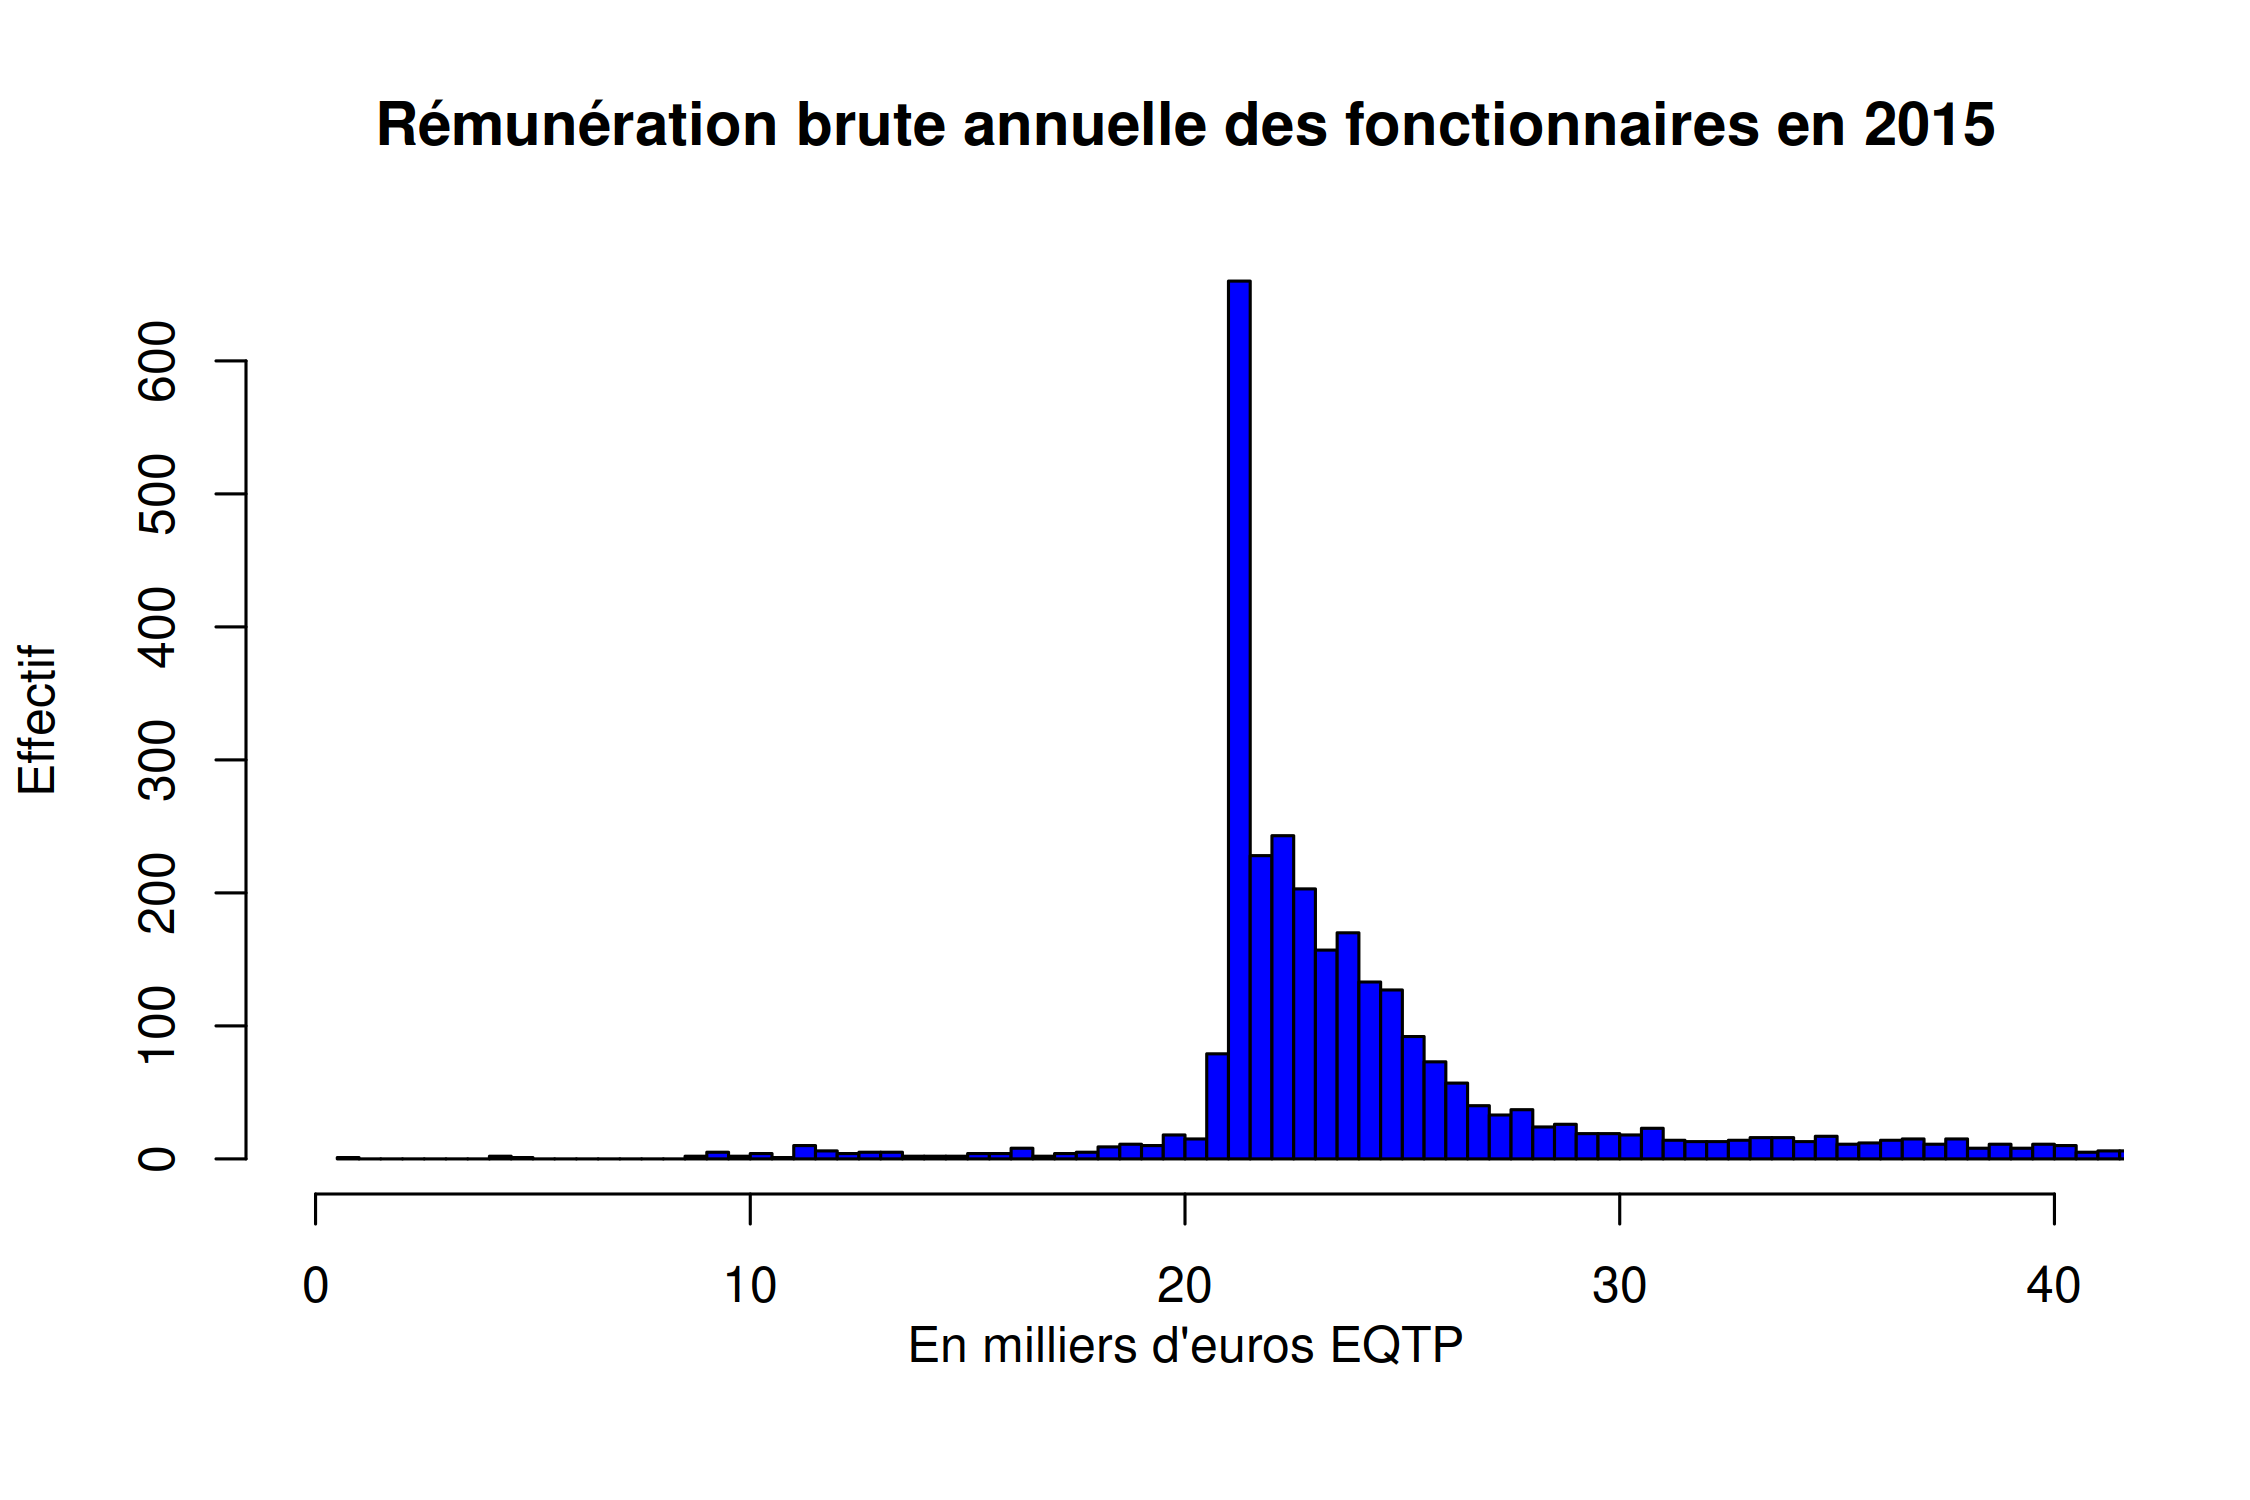
\includegraphics{altair_files/figure-latex/unnamed-chunk-76-1.png}

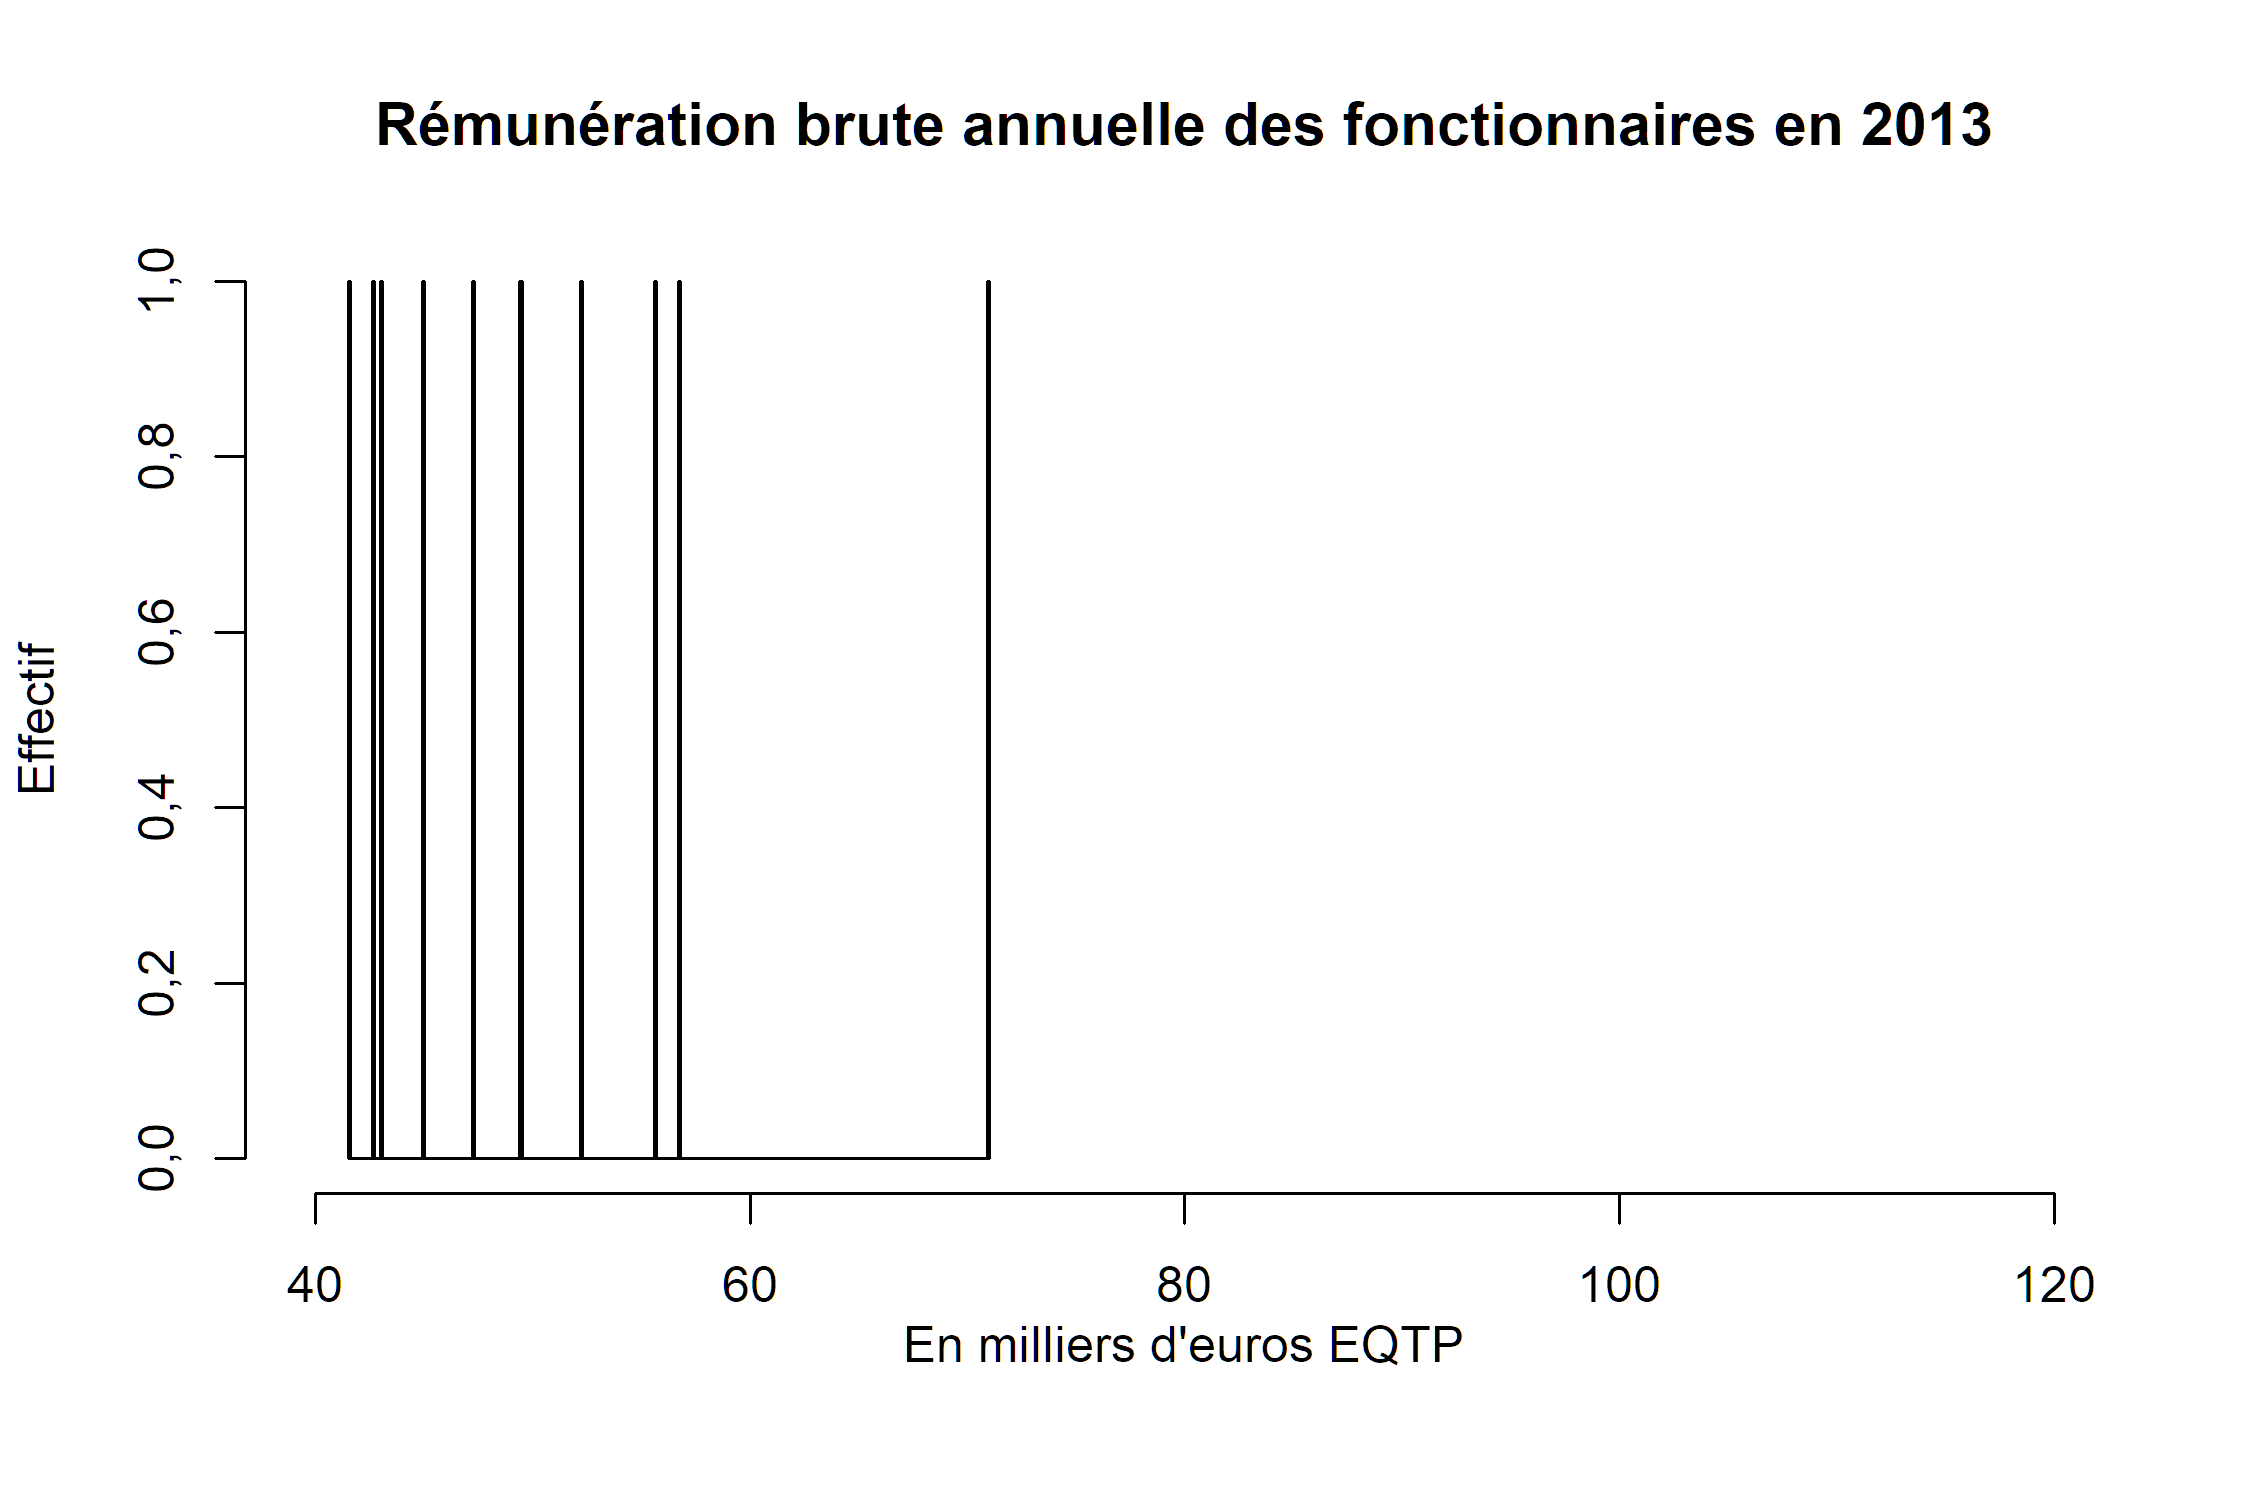
\includegraphics{altair_files/figure-latex/unnamed-chunk-76-2.png}

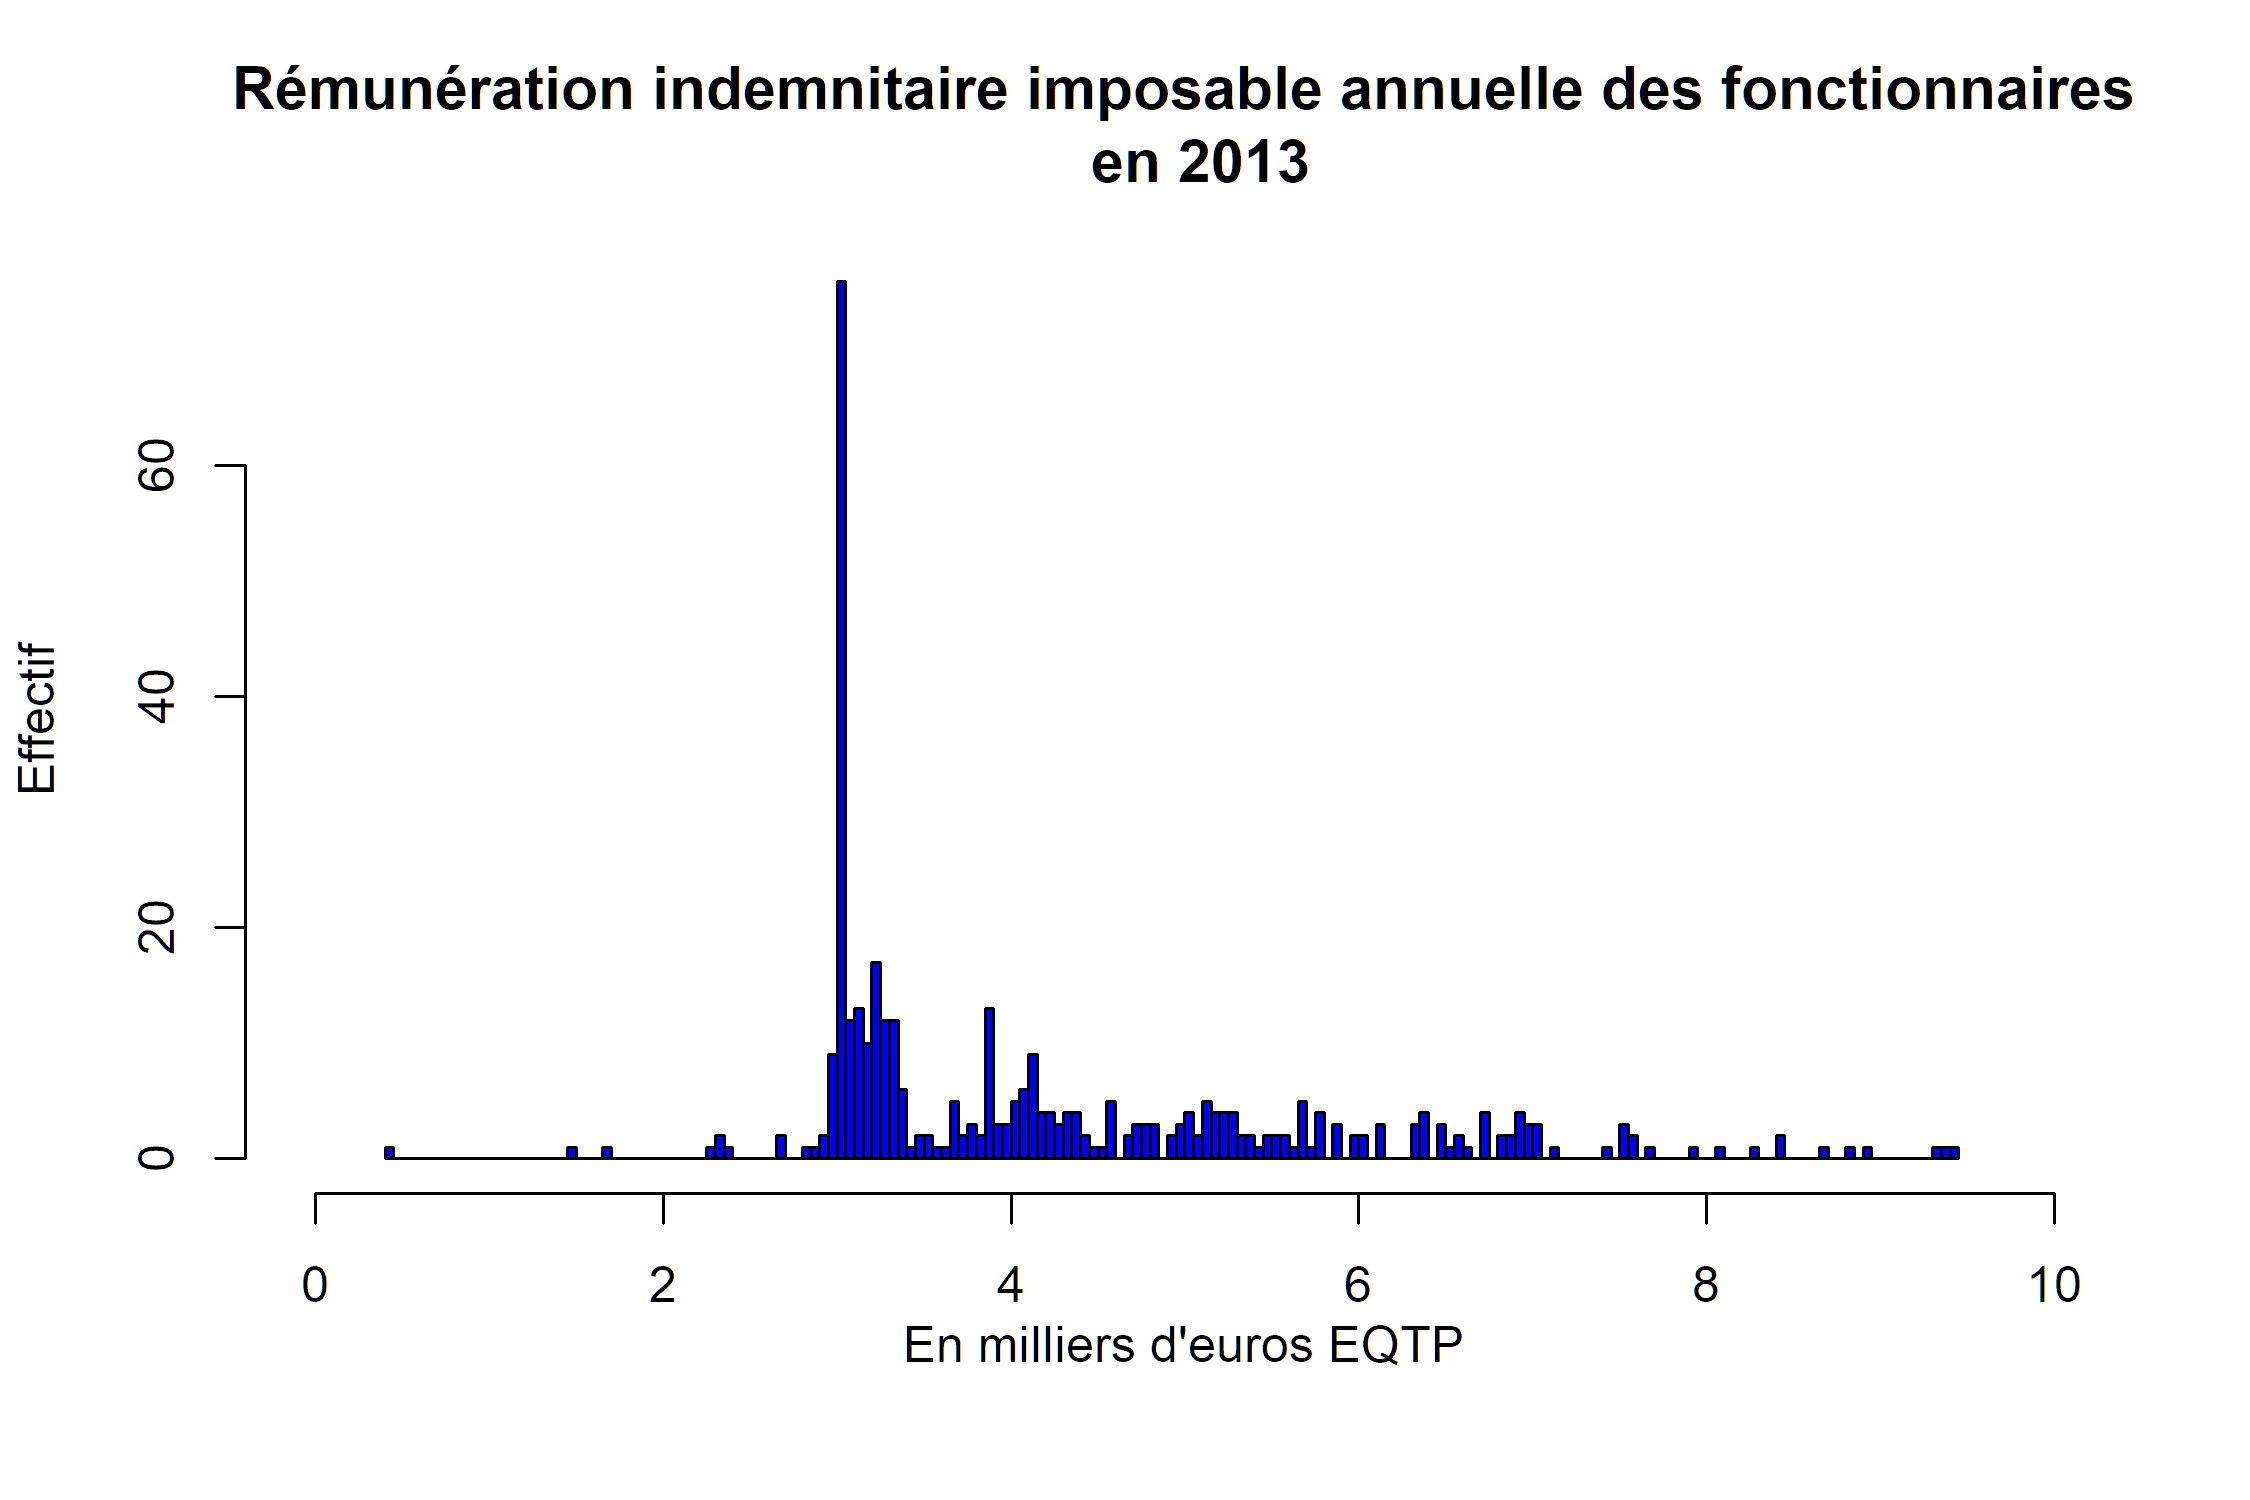
\includegraphics{altair_files/figure-latex/unnamed-chunk-76-3.png}

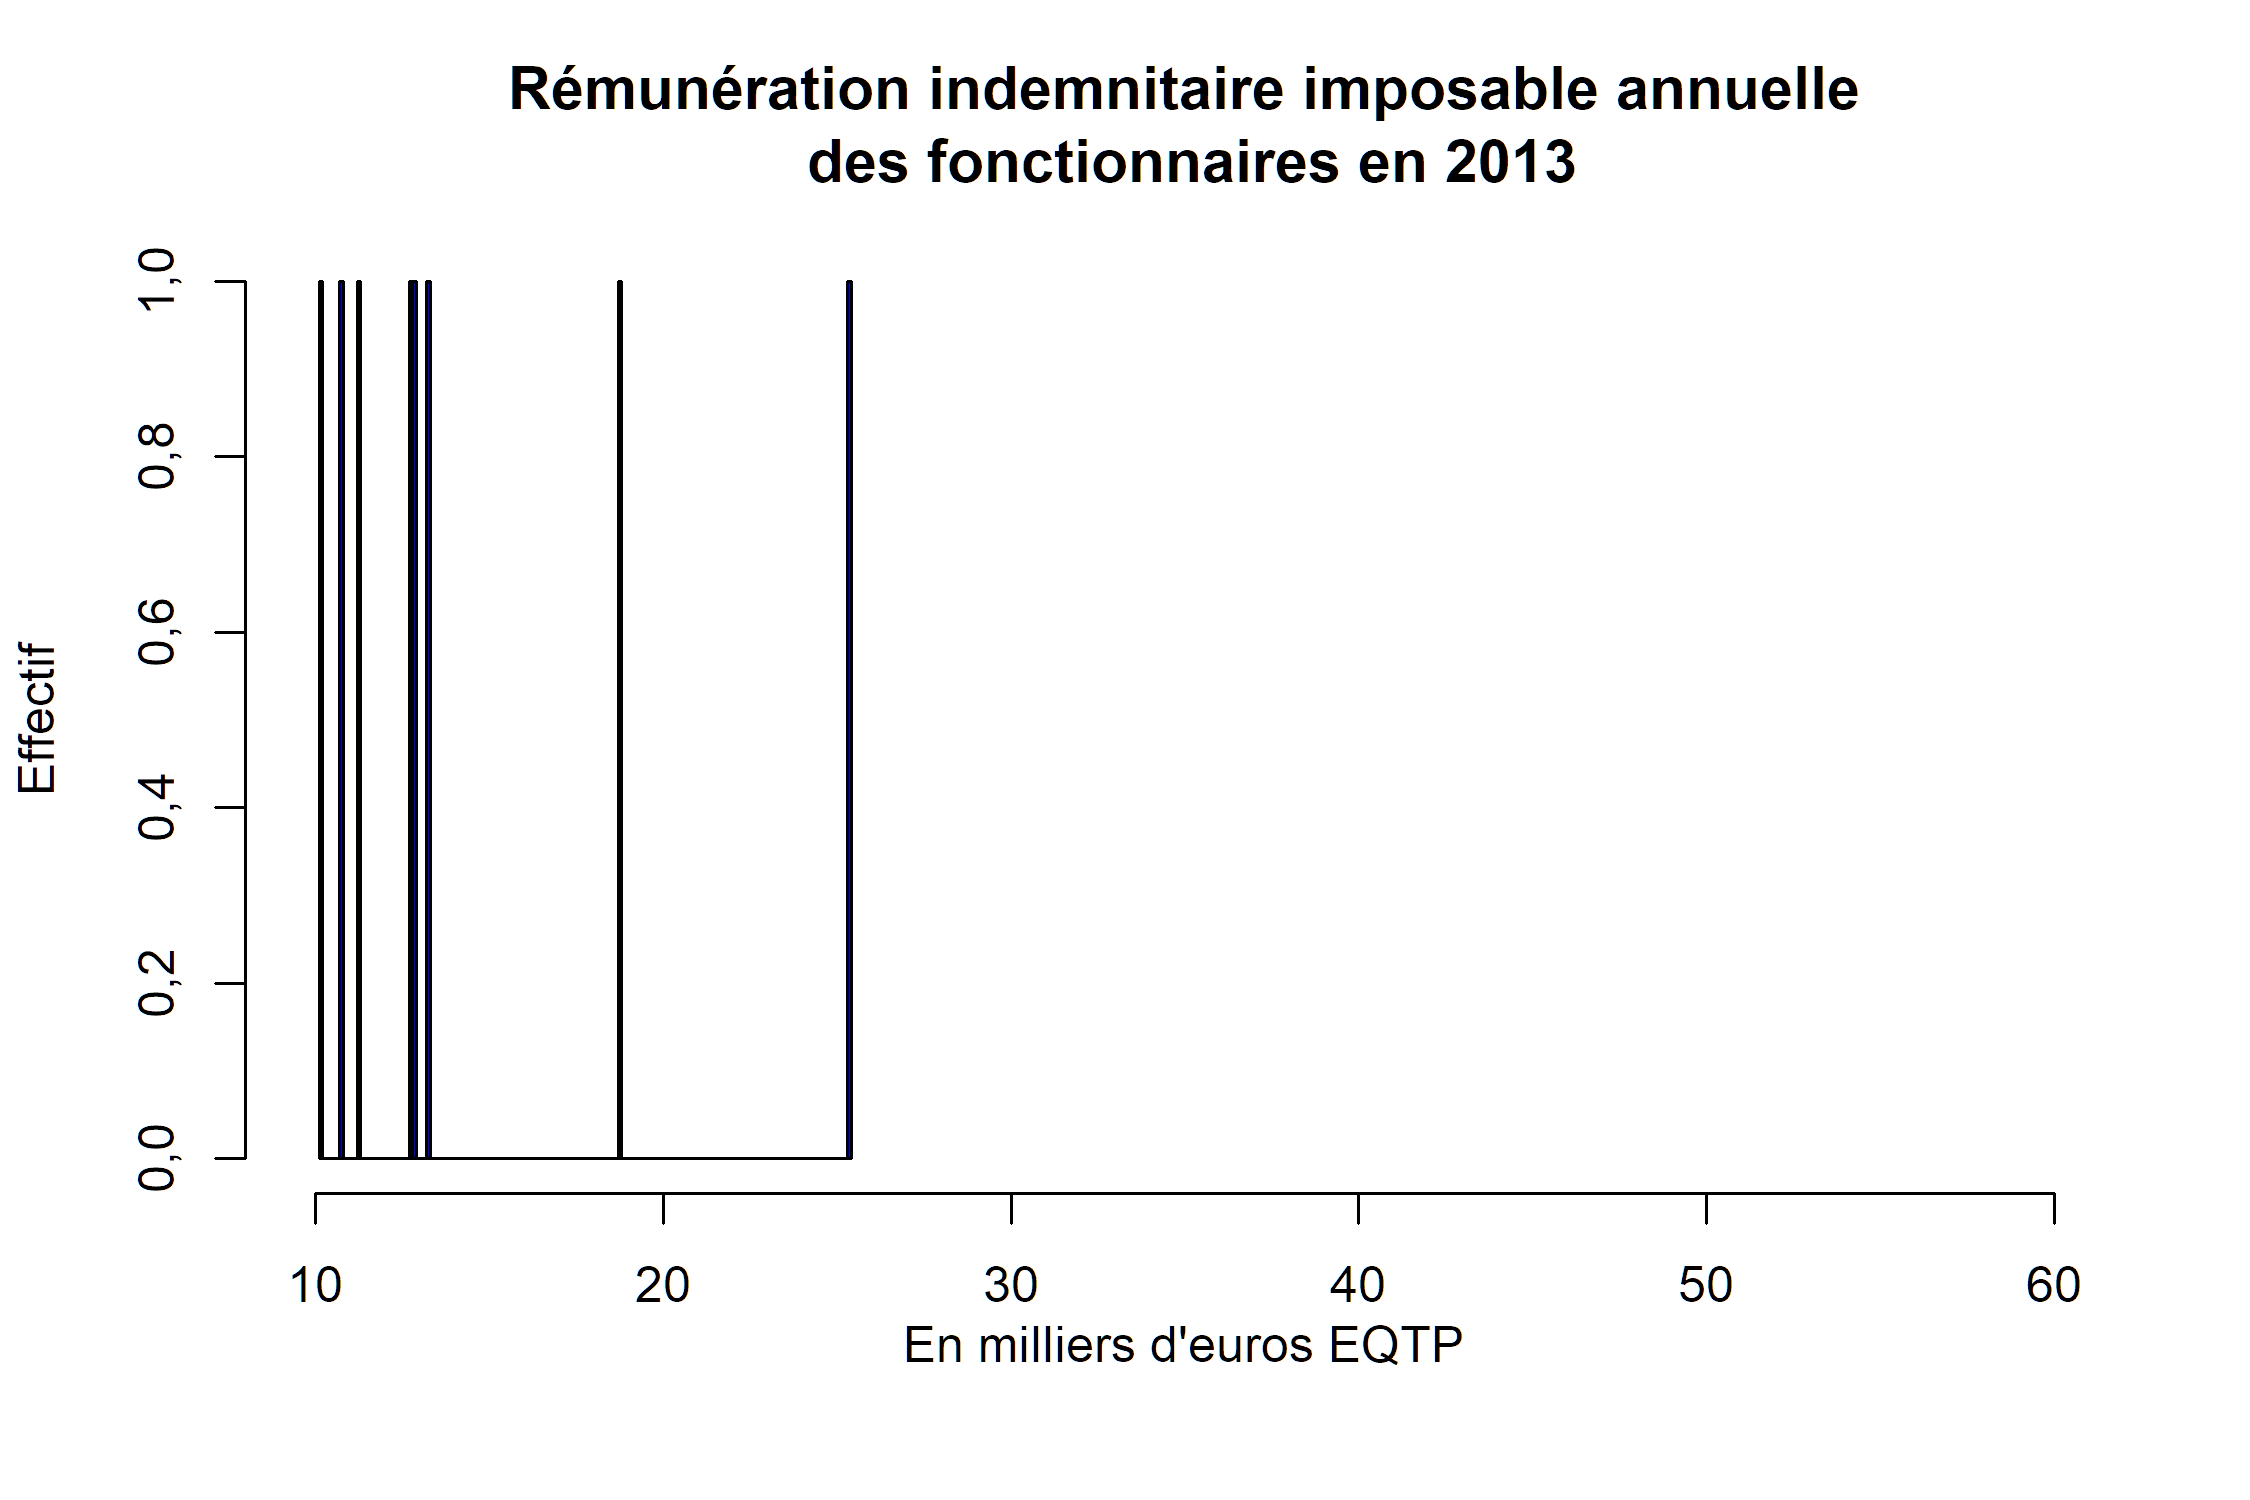
\includegraphics{altair_files/figure-latex/unnamed-chunk-76-4.png}

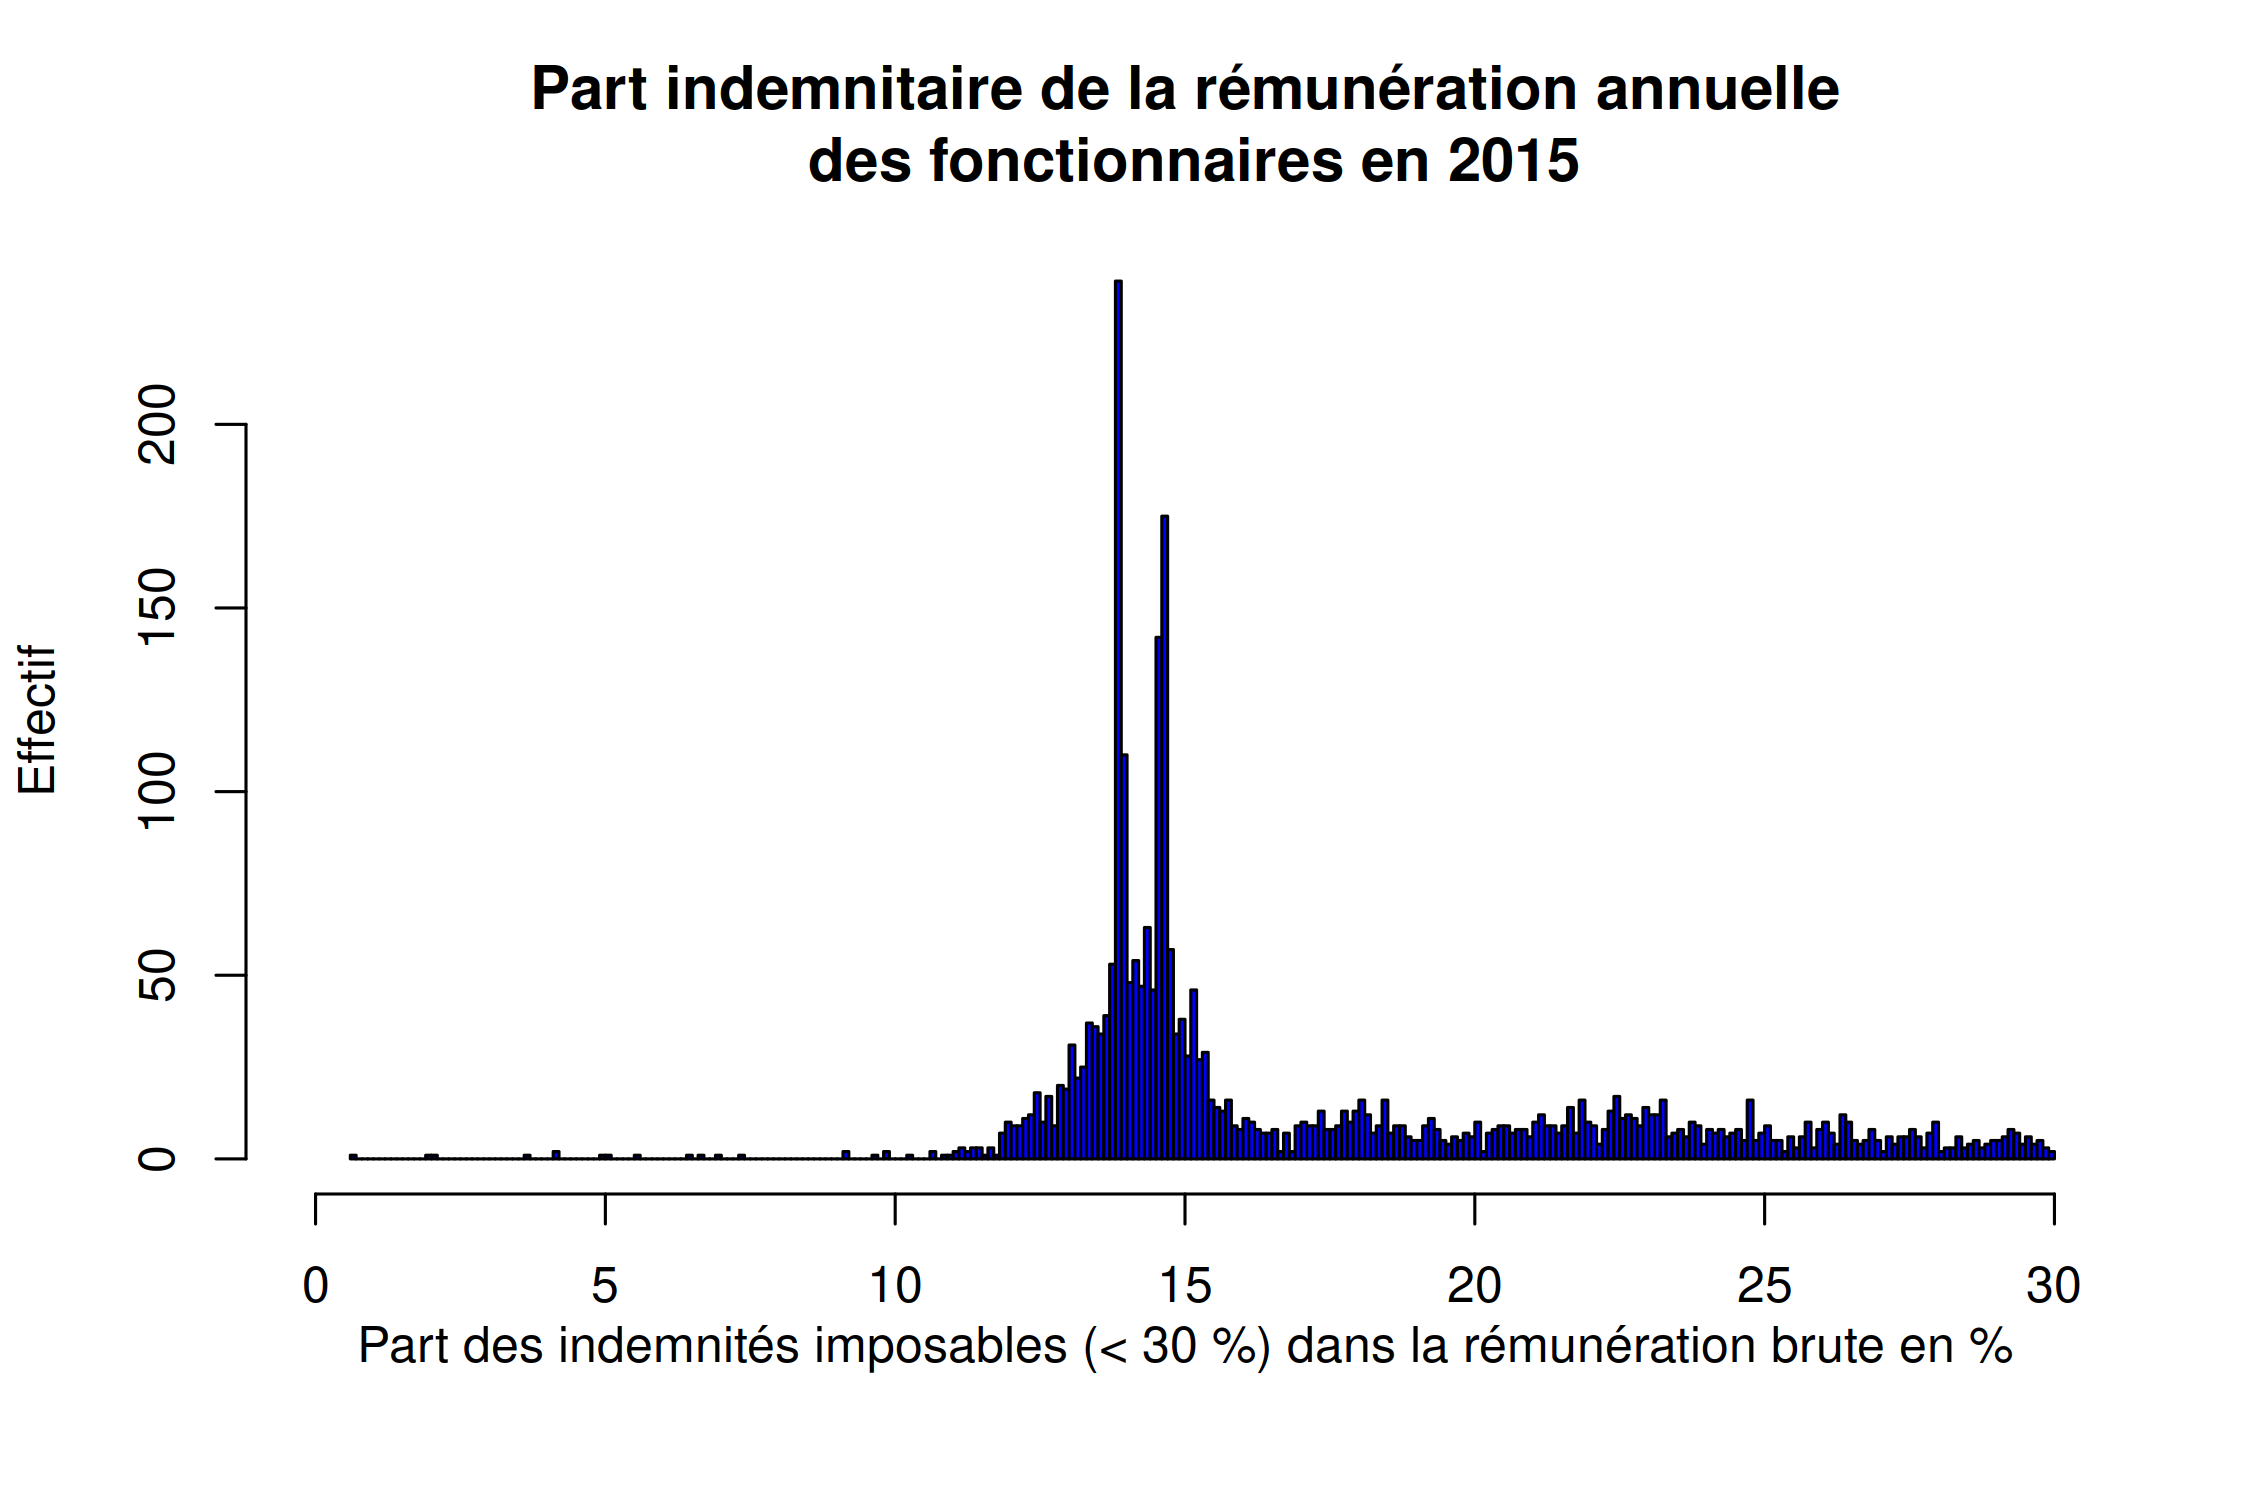
\includegraphics{altair_files/figure-latex/unnamed-chunk-76-5.png}

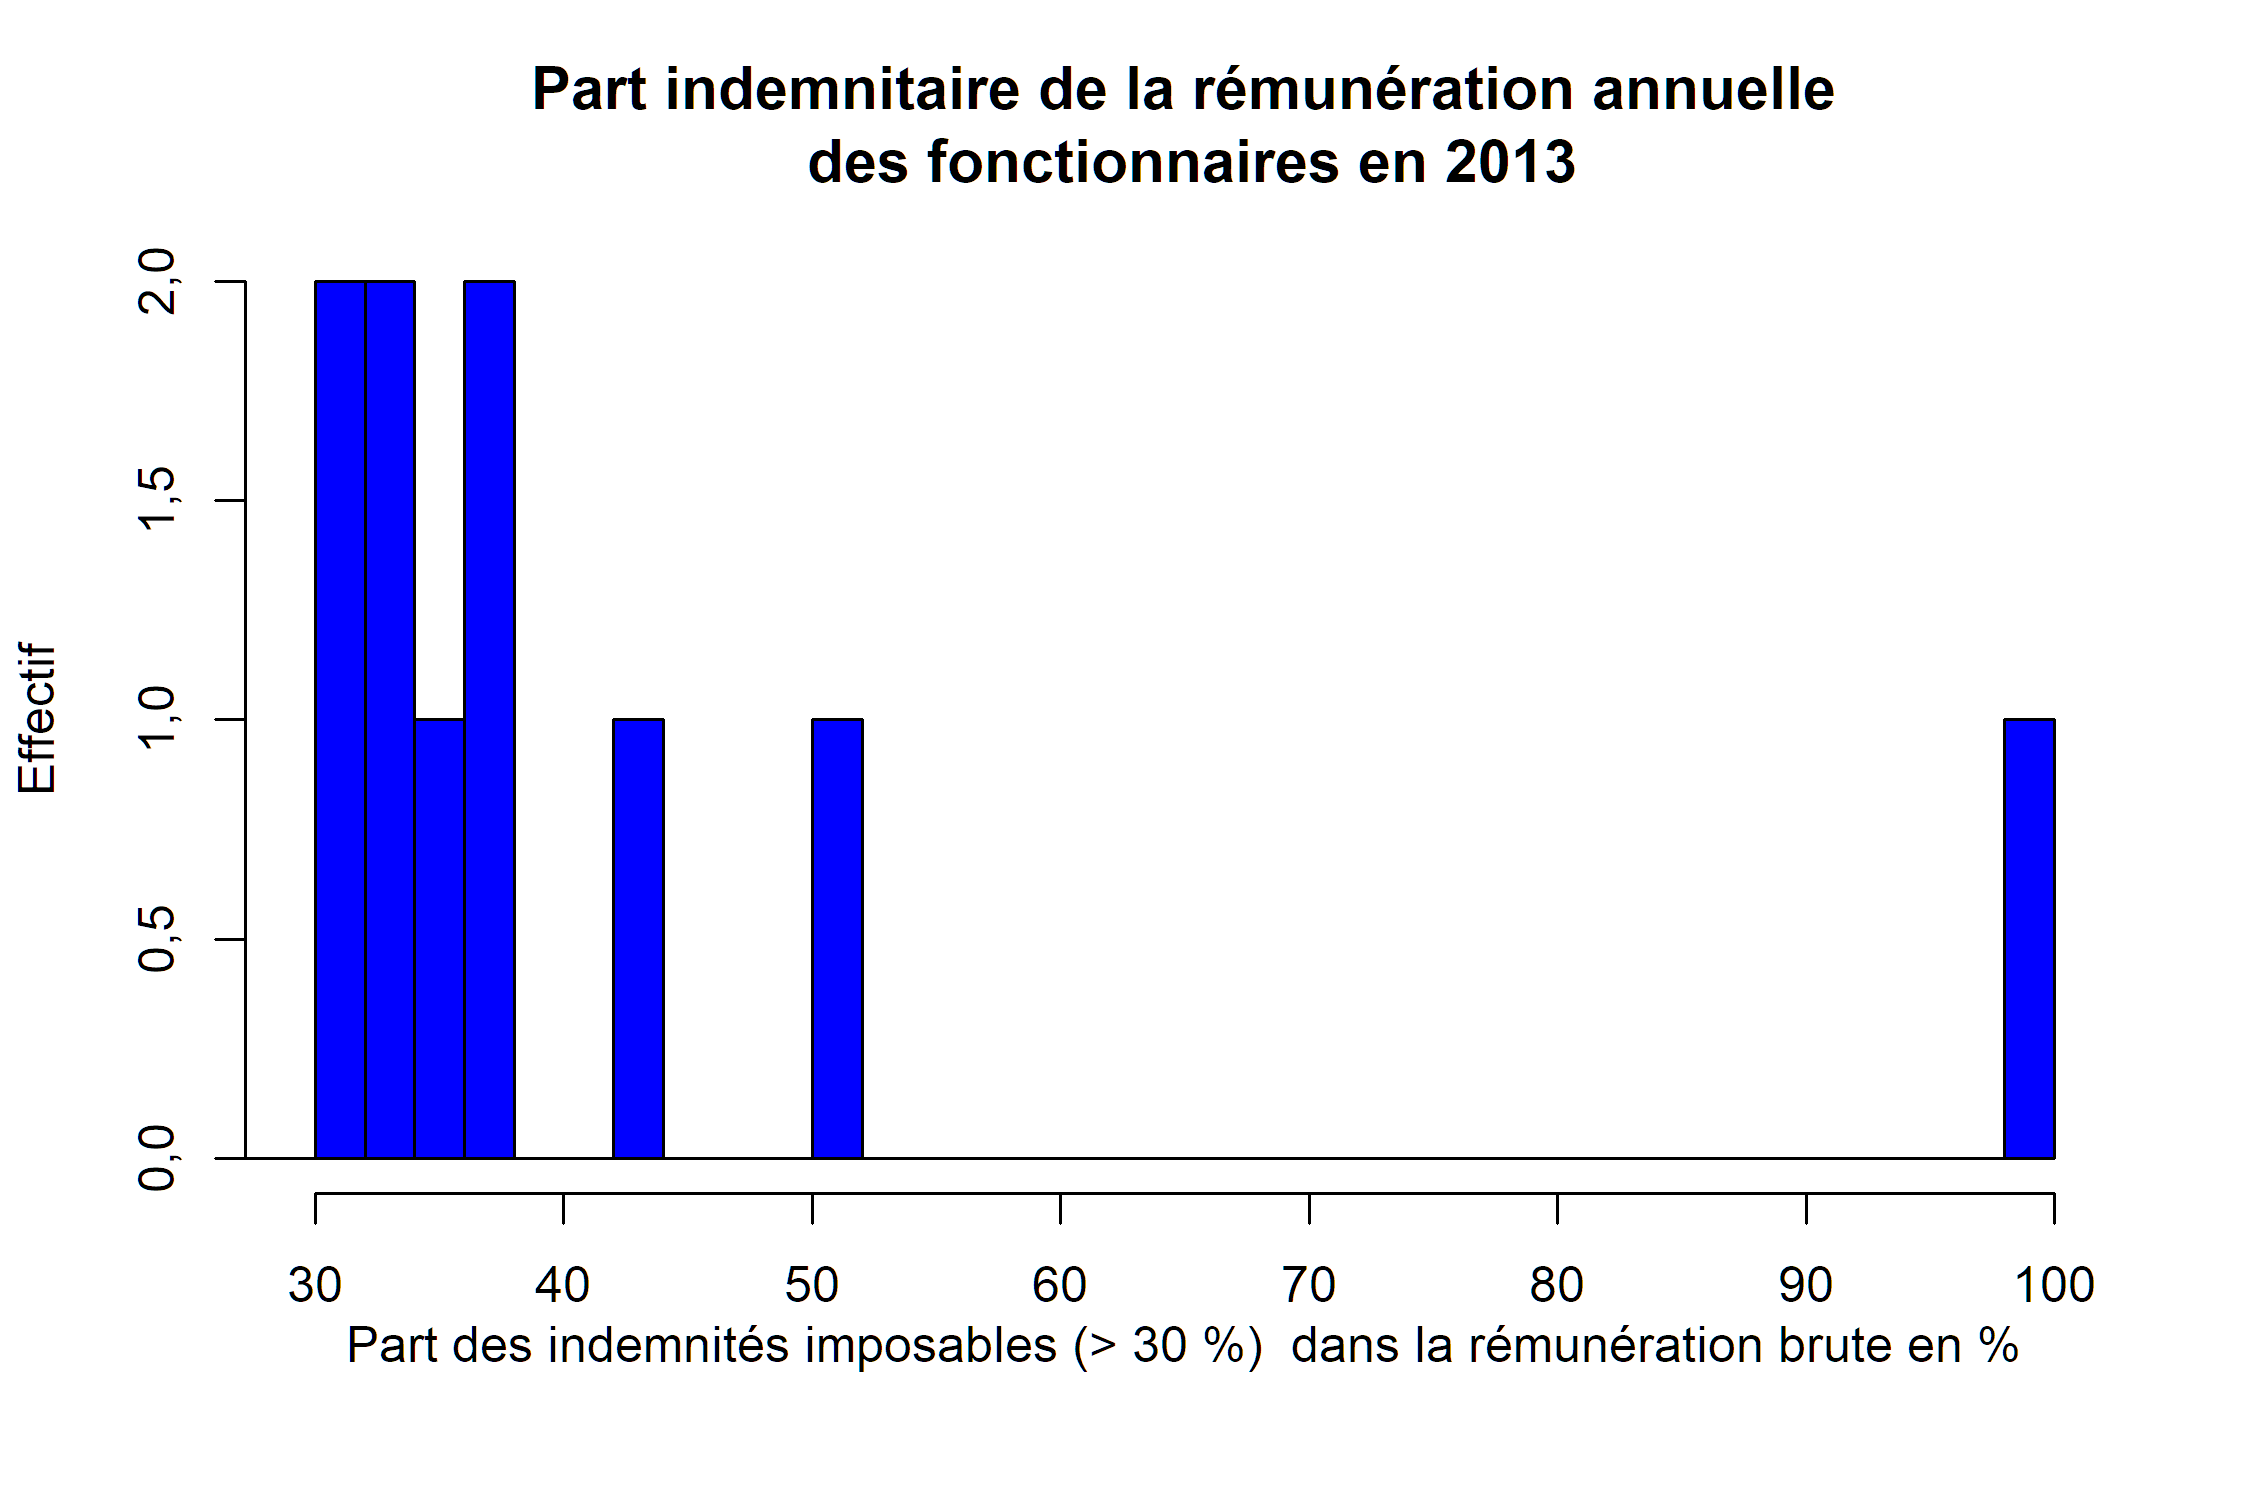
\includegraphics{altair_files/figure-latex/unnamed-chunk-76-6.png}

\textbf{Nota :}\\
\emph{Cet histogramme décrit l'évolution de la rémunération moyenne des
personnes en place (RMPP), définies comme présentes deux annees entières
consécutives avec la même quotité}\\
\emph{L'évolution de la RMPP permet d'étudier le glissement
vieillesse-technicité ``positif'', à effectifs constants sur deux
années}

\textbf{Effectif : 411 }

\textbf{Tests de cohérence}

Somme des rémunérations brutes versées aux personnels titulaires et
stagiaires :

~\emph{Tableau 3.2.1}

\begin{longtable}[]{@{}ll@{}}
\toprule
Agrégats & k€\tabularnewline
\midrule
\endhead
Brut annuel (bulletins) & 9 511 343,6\tabularnewline
Brut annuel (lignes) : & 9 520 372,0\tabularnewline
~dont ~~primes : & 1 662 312,8\tabularnewline
~dont ~autres rémunérations : &\tabularnewline
Part de primes en \% & 17,5\tabularnewline
\bottomrule
\end{longtable}

\textbf{Définitions :}

\emph{Brut annuel (bulletins)} : somme du champ \emph{Brut}\\
\emph{Brut annuel (lignes)} : somme du champ \emph{Montant} des lignes
de paye, dont :\\
\emph{Primes} : indemnités sauf remboursements, certaines IJSS,
Supplément familial de traitement et Indemnité de résidence\\
\emph{Autres rémunérations} : acomptes, retenues sur brut, rémunérations
diverses, rappels

\textbf{Tests de cohérence}

Somme des rémunérations brutes versées aux personnels (fonctionnaires) :

~\emph{Tableau 3.2.2}

\begin{longtable}[]{@{}ll@{}}
\toprule
Agrégats & k€\tabularnewline
\midrule
\endhead
Bulletins de paie & 9 511 343,6\tabularnewline
Lignes de paie & 9 520 372,0\tabularnewline
Difference & -9 028,3\tabularnewline
\bottomrule
\end{longtable}

A comparer aux soldes des comptes 6411, 6419 et 648 du compte de
gestion.

\textbf{Formation et distribution du salaire brut moyen par tête (SMPT)
en EQTP pour l'année 2013 }

~\emph{Tableau 3.2.3}

\begin{longtable}[]{@{}rrrrrr@{}}
\toprule
\begin{minipage}[b]{0.14\columnwidth}\raggedleft
Statistique\strut
\end{minipage} & \begin{minipage}[b]{0.23\columnwidth}\raggedleft
Traitement indiciaire\strut
\end{minipage} & \begin{minipage}[b]{0.07\columnwidth}\raggedleft
Primes\strut
\end{minipage} & \begin{minipage}[b]{0.22\columnwidth}\raggedleft
Autres rémunérations\strut
\end{minipage} & \begin{minipage}[b]{0.08\columnwidth}\raggedleft
Quotité\strut
\end{minipage} & \begin{minipage}[b]{0.09\columnwidth}\raggedleft
Effectif\strut
\end{minipage}\tabularnewline
\midrule
\endhead
\begin{minipage}[t]{0.14\columnwidth}\raggedleft
Minimum\strut
\end{minipage} & \begin{minipage}[t]{0.23\columnwidth}\raggedleft
8 666\strut
\end{minipage} & \begin{minipage}[t]{0.07\columnwidth}\raggedleft
1 363\strut
\end{minipage} & \begin{minipage}[t]{0.22\columnwidth}\raggedleft
0\strut
\end{minipage} & \begin{minipage}[t]{0.08\columnwidth}\raggedleft
0,45\strut
\end{minipage} & \begin{minipage}[t]{0.09\columnwidth}\raggedleft
\strut
\end{minipage}\tabularnewline
\begin{minipage}[t]{0.14\columnwidth}\raggedleft
1er quartile\strut
\end{minipage} & \begin{minipage}[t]{0.23\columnwidth}\raggedleft
17 438\strut
\end{minipage} & \begin{minipage}[t]{0.07\columnwidth}\raggedleft
3 023\strut
\end{minipage} & \begin{minipage}[t]{0.22\columnwidth}\raggedleft
0\strut
\end{minipage} & \begin{minipage}[t]{0.08\columnwidth}\raggedleft
1\strut
\end{minipage} & \begin{minipage}[t]{0.09\columnwidth}\raggedleft
\strut
\end{minipage}\tabularnewline
\begin{minipage}[t]{0.14\columnwidth}\raggedleft
Médiane\strut
\end{minipage} & \begin{minipage}[t]{0.23\columnwidth}\raggedleft
18 614\strut
\end{minipage} & \begin{minipage}[t]{0.07\columnwidth}\raggedleft
3 399\strut
\end{minipage} & \begin{minipage}[t]{0.22\columnwidth}\raggedleft
0\strut
\end{minipage} & \begin{minipage}[t]{0.08\columnwidth}\raggedleft
1\strut
\end{minipage} & \begin{minipage}[t]{0.09\columnwidth}\raggedleft
\strut
\end{minipage}\tabularnewline
\begin{minipage}[t]{0.14\columnwidth}\raggedleft
Moyenne\strut
\end{minipage} & \begin{minipage}[t]{0.23\columnwidth}\raggedleft
20 015\strut
\end{minipage} & \begin{minipage}[t]{0.07\columnwidth}\raggedleft
4 253\strut
\end{minipage} & \begin{minipage}[t]{0.22\columnwidth}\raggedleft
0\strut
\end{minipage} & \begin{minipage}[t]{0.08\columnwidth}\raggedleft
0,96\strut
\end{minipage} & \begin{minipage}[t]{0.09\columnwidth}\raggedleft
395\strut
\end{minipage}\tabularnewline
\begin{minipage}[t]{0.14\columnwidth}\raggedleft
3ème quartile\strut
\end{minipage} & \begin{minipage}[t]{0.23\columnwidth}\raggedleft
21 892\strut
\end{minipage} & \begin{minipage}[t]{0.07\columnwidth}\raggedleft
4 936\strut
\end{minipage} & \begin{minipage}[t]{0.22\columnwidth}\raggedleft
0\strut
\end{minipage} & \begin{minipage}[t]{0.08\columnwidth}\raggedleft
1\strut
\end{minipage} & \begin{minipage}[t]{0.09\columnwidth}\raggedleft
\strut
\end{minipage}\tabularnewline
\begin{minipage}[t]{0.14\columnwidth}\raggedleft
Maximum\strut
\end{minipage} & \begin{minipage}[t]{0.23\columnwidth}\raggedleft
47 256\strut
\end{minipage} & \begin{minipage}[t]{0.07\columnwidth}\raggedleft
25 307\strut
\end{minipage} & \begin{minipage}[t]{0.22\columnwidth}\raggedleft
0\strut
\end{minipage} & \begin{minipage}[t]{0.08\columnwidth}\raggedleft
1\strut
\end{minipage} & \begin{minipage}[t]{0.09\columnwidth}\raggedleft
\strut
\end{minipage}\tabularnewline
\bottomrule
\end{longtable}

~\emph{Tableau 3.2.4}

\begin{longtable}[]{@{}rrrrrrr@{}}
\toprule
\begin{minipage}[b]{0.11\columnwidth}\raggedleft
Statistique\strut
\end{minipage} & \begin{minipage}[b]{0.20\columnwidth}\raggedleft
Total lignes hors rappels\strut
\end{minipage} & \begin{minipage}[b]{0.09\columnwidth}\raggedleft
Total brut\strut
\end{minipage} & \begin{minipage}[b]{0.14\columnwidth}\raggedleft
SMPT brut en EQTP\strut
\end{minipage} & \begin{minipage}[b]{0.14\columnwidth}\raggedleft
Part indemnitaire\strut
\end{minipage} & \begin{minipage}[b]{0.06\columnwidth}\raggedleft
Quotité\strut
\end{minipage} & \begin{minipage}[b]{0.07\columnwidth}\raggedleft
Effectif\strut
\end{minipage}\tabularnewline
\midrule
\endhead
\begin{minipage}[t]{0.11\columnwidth}\raggedleft
Minimum\strut
\end{minipage} & \begin{minipage}[t]{0.20\columnwidth}\raggedleft
5 946\strut
\end{minipage} & \begin{minipage}[t]{0.09\columnwidth}\raggedleft
5 946\strut
\end{minipage} & \begin{minipage}[t]{0.14\columnwidth}\raggedleft
10 547\strut
\end{minipage} & \begin{minipage}[t]{0.14\columnwidth}\raggedleft
10\strut
\end{minipage} & \begin{minipage}[t]{0.06\columnwidth}\raggedleft
0,45\strut
\end{minipage} & \begin{minipage}[t]{0.07\columnwidth}\raggedleft
\strut
\end{minipage}\tabularnewline
\begin{minipage}[t]{0.11\columnwidth}\raggedleft
1er quartile\strut
\end{minipage} & \begin{minipage}[t]{0.20\columnwidth}\raggedleft
20 802\strut
\end{minipage} & \begin{minipage}[t]{0.09\columnwidth}\raggedleft
20 869\strut
\end{minipage} & \begin{minipage}[t]{0.14\columnwidth}\raggedleft
20 878\strut
\end{minipage} & \begin{minipage}[t]{0.14\columnwidth}\raggedleft
14\strut
\end{minipage} & \begin{minipage}[t]{0.06\columnwidth}\raggedleft
1\strut
\end{minipage} & \begin{minipage}[t]{0.07\columnwidth}\raggedleft
\strut
\end{minipage}\tabularnewline
\begin{minipage}[t]{0.11\columnwidth}\raggedleft
Médiane\strut
\end{minipage} & \begin{minipage}[t]{0.20\columnwidth}\raggedleft
22 941\strut
\end{minipage} & \begin{minipage}[t]{0.09\columnwidth}\raggedleft
22 962\strut
\end{minipage} & \begin{minipage}[t]{0.14\columnwidth}\raggedleft
23 019\strut
\end{minipage} & \begin{minipage}[t]{0.14\columnwidth}\raggedleft
16\strut
\end{minipage} & \begin{minipage}[t]{0.06\columnwidth}\raggedleft
1\strut
\end{minipage} & \begin{minipage}[t]{0.07\columnwidth}\raggedleft
\strut
\end{minipage}\tabularnewline
\begin{minipage}[t]{0.11\columnwidth}\raggedleft
Moyenne\strut
\end{minipage} & \begin{minipage}[t]{0.20\columnwidth}\raggedleft
24 510\strut
\end{minipage} & \begin{minipage}[t]{0.09\columnwidth}\raggedleft
24 488\strut
\end{minipage} & \begin{minipage}[t]{0.14\columnwidth}\raggedleft
24 613\strut
\end{minipage} & \begin{minipage}[t]{0.14\columnwidth}\raggedleft
17\strut
\end{minipage} & \begin{minipage}[t]{0.06\columnwidth}\raggedleft
0,96\strut
\end{minipage} & \begin{minipage}[t]{0.07\columnwidth}\raggedleft
395\strut
\end{minipage}\tabularnewline
\begin{minipage}[t]{0.11\columnwidth}\raggedleft
3ème quartile\strut
\end{minipage} & \begin{minipage}[t]{0.20\columnwidth}\raggedleft
27 108\strut
\end{minipage} & \begin{minipage}[t]{0.09\columnwidth}\raggedleft
27 109\strut
\end{minipage} & \begin{minipage}[t]{0.14\columnwidth}\raggedleft
27 109\strut
\end{minipage} & \begin{minipage}[t]{0.14\columnwidth}\raggedleft
20\strut
\end{minipage} & \begin{minipage}[t]{0.06\columnwidth}\raggedleft
1\strut
\end{minipage} & \begin{minipage}[t]{0.07\columnwidth}\raggedleft
\strut
\end{minipage}\tabularnewline
\begin{minipage}[t]{0.11\columnwidth}\raggedleft
Maximum\strut
\end{minipage} & \begin{minipage}[t]{0.20\columnwidth}\raggedleft
70 925\strut
\end{minipage} & \begin{minipage}[t]{0.09\columnwidth}\raggedleft
70 925\strut
\end{minipage} & \begin{minipage}[t]{0.14\columnwidth}\raggedleft
70 925\strut
\end{minipage} & \begin{minipage}[t]{0.14\columnwidth}\raggedleft
49\strut
\end{minipage} & \begin{minipage}[t]{0.06\columnwidth}\raggedleft
1\strut
\end{minipage} & \begin{minipage}[t]{0.07\columnwidth}\raggedleft
\strut
\end{minipage}\tabularnewline
\bottomrule
\end{longtable}

\emph{Hors vacataires identifiés, assistantes maternelles, élus locaux
et pour les postes actifs non annexes}

\textbf{Categorie A}

~\emph{Tableau 3.2.5}

\begin{longtable}[]{@{}rrrrr@{}}
\toprule
Statistique & Traitement indiciaire & Primes & Autres rémunérations &
Quotité\tabularnewline
\midrule
\endhead
Minimum & 21 275 & 5 783 & 0 & 0,7\tabularnewline
1er quartile & 26 467 & 7 424 & 0 & 1\tabularnewline
Médiane & 30 426 & 8 862 & 0 & 1\tabularnewline
Moyenne & 32 383 & 10 091 & 0 & 0,97\tabularnewline
3ème quartile & 39 891 & 10 746 & 0 & 1\tabularnewline
Maximum & 47 256 & 25 307 & 0 & 1\tabularnewline
\bottomrule
\end{longtable}

~\emph{Tableau 3.2.6}

\begin{longtable}[]{@{}rrrrr@{}}
\toprule
\begin{minipage}[b]{0.14\columnwidth}\raggedleft
Statistique\strut
\end{minipage} & \begin{minipage}[b]{0.20\columnwidth}\raggedleft
Total rémunérations\strut
\end{minipage} & \begin{minipage}[b]{0.25\columnwidth}\raggedleft
Total rémunérations EQTP\strut
\end{minipage} & \begin{minipage}[b]{0.18\columnwidth}\raggedleft
Part indemnitaire\strut
\end{minipage} & \begin{minipage}[b]{0.08\columnwidth}\raggedleft
Quotité\strut
\end{minipage}\tabularnewline
\midrule
\endhead
\begin{minipage}[t]{0.14\columnwidth}\raggedleft
Minimum\strut
\end{minipage} & \begin{minipage}[t]{0.20\columnwidth}\raggedleft
27 166\strut
\end{minipage} & \begin{minipage}[t]{0.25\columnwidth}\raggedleft
27 166\strut
\end{minipage} & \begin{minipage}[t]{0.18\columnwidth}\raggedleft
17\strut
\end{minipage} & \begin{minipage}[t]{0.08\columnwidth}\raggedleft
0,7\strut
\end{minipage}\tabularnewline
\begin{minipage}[t]{0.14\columnwidth}\raggedleft
1er quartile\strut
\end{minipage} & \begin{minipage}[t]{0.20\columnwidth}\raggedleft
35 566\strut
\end{minipage} & \begin{minipage}[t]{0.25\columnwidth}\raggedleft
35 566\strut
\end{minipage} & \begin{minipage}[t]{0.18\columnwidth}\raggedleft
19\strut
\end{minipage} & \begin{minipage}[t]{0.08\columnwidth}\raggedleft
1\strut
\end{minipage}\tabularnewline
\begin{minipage}[t]{0.14\columnwidth}\raggedleft
Médiane\strut
\end{minipage} & \begin{minipage}[t]{0.20\columnwidth}\raggedleft
37 648\strut
\end{minipage} & \begin{minipage}[t]{0.25\columnwidth}\raggedleft
40 002\strut
\end{minipage} & \begin{minipage}[t]{0.18\columnwidth}\raggedleft
23\strut
\end{minipage} & \begin{minipage}[t]{0.08\columnwidth}\raggedleft
1\strut
\end{minipage}\tabularnewline
\begin{minipage}[t]{0.14\columnwidth}\raggedleft
Moyenne\strut
\end{minipage} & \begin{minipage}[t]{0.20\columnwidth}\raggedleft
41 987\strut
\end{minipage} & \begin{minipage}[t]{0.25\columnwidth}\raggedleft
42 340\strut
\end{minipage} & \begin{minipage}[t]{0.18\columnwidth}\raggedleft
23\strut
\end{minipage} & \begin{minipage}[t]{0.08\columnwidth}\raggedleft
0,97\strut
\end{minipage}\tabularnewline
\begin{minipage}[t]{0.14\columnwidth}\raggedleft
3ème quartile\strut
\end{minipage} & \begin{minipage}[t]{0.20\columnwidth}\raggedleft
49 870\strut
\end{minipage} & \begin{minipage}[t]{0.25\columnwidth}\raggedleft
49 870\strut
\end{minipage} & \begin{minipage}[t]{0.18\columnwidth}\raggedleft
26\strut
\end{minipage} & \begin{minipage}[t]{0.08\columnwidth}\raggedleft
1\strut
\end{minipage}\tabularnewline
\begin{minipage}[t]{0.14\columnwidth}\raggedleft
Maximum\strut
\end{minipage} & \begin{minipage}[t]{0.20\columnwidth}\raggedleft
70 925\strut
\end{minipage} & \begin{minipage}[t]{0.25\columnwidth}\raggedleft
70 925\strut
\end{minipage} & \begin{minipage}[t]{0.18\columnwidth}\raggedleft
36\strut
\end{minipage} & \begin{minipage}[t]{0.08\columnwidth}\raggedleft
1\strut
\end{minipage}\tabularnewline
\bottomrule
\end{longtable}

\textbf{Effectif : 18 }

\textbf{Categorie B}

~\emph{Tableau 3.2.7}

\begin{longtable}[]{@{}rrrrr@{}}
\toprule
Statistique & Traitement indiciaire & Primes & Autres rémunérations &
Quotité\tabularnewline
\midrule
\endhead
Minimum & 11 908 & 3 358 & 0 & 0,51\tabularnewline
1er quartile & 20 833 & 5 132 & 0 & 0,95\tabularnewline
Médiane & 23 500 & 5 473 & 0 & 1\tabularnewline
Moyenne & 23 273 & 5 859 & 0 & 0,94\tabularnewline
3ème quartile & 25 992 & 6 360 & 0 & 1\tabularnewline
Maximum & 33 338 & 12 899 & 0 & 1\tabularnewline
\bottomrule
\end{longtable}

~\emph{Tableau 3.2.8}

\begin{longtable}[]{@{}rrrrr@{}}
\toprule
\begin{minipage}[b]{0.12\columnwidth}\raggedleft
Statistique\strut
\end{minipage} & \begin{minipage}[b]{0.17\columnwidth}\raggedleft
Total rémunérations\strut
\end{minipage} & \begin{minipage}[b]{0.21\columnwidth}\raggedleft
Total rémunérations EQTP\strut
\end{minipage} & \begin{minipage}[b]{0.31\columnwidth}\raggedleft
Part de la rémunération indemnitaire\strut
\end{minipage} & \begin{minipage}[b]{0.07\columnwidth}\raggedleft
Quotité\strut
\end{minipage}\tabularnewline
\midrule
\endhead
\begin{minipage}[t]{0.12\columnwidth}\raggedleft
Minimum\strut
\end{minipage} & \begin{minipage}[t]{0.17\columnwidth}\raggedleft
15 643\strut
\end{minipage} & \begin{minipage}[t]{0.21\columnwidth}\raggedleft
16 695\strut
\end{minipage} & \begin{minipage}[t]{0.31\columnwidth}\raggedleft
13\strut
\end{minipage} & \begin{minipage}[t]{0.07\columnwidth}\raggedleft
0,51\strut
\end{minipage}\tabularnewline
\begin{minipage}[t]{0.12\columnwidth}\raggedleft
1er quartile\strut
\end{minipage} & \begin{minipage}[t]{0.17\columnwidth}\raggedleft
26 303\strut
\end{minipage} & \begin{minipage}[t]{0.21\columnwidth}\raggedleft
26 303\strut
\end{minipage} & \begin{minipage}[t]{0.31\columnwidth}\raggedleft
17\strut
\end{minipage} & \begin{minipage}[t]{0.07\columnwidth}\raggedleft
0,95\strut
\end{minipage}\tabularnewline
\begin{minipage}[t]{0.12\columnwidth}\raggedleft
Médiane\strut
\end{minipage} & \begin{minipage}[t]{0.17\columnwidth}\raggedleft
29 410\strut
\end{minipage} & \begin{minipage}[t]{0.21\columnwidth}\raggedleft
29 410\strut
\end{minipage} & \begin{minipage}[t]{0.31\columnwidth}\raggedleft
20\strut
\end{minipage} & \begin{minipage}[t]{0.07\columnwidth}\raggedleft
1\strut
\end{minipage}\tabularnewline
\begin{minipage}[t]{0.12\columnwidth}\raggedleft
Moyenne\strut
\end{minipage} & \begin{minipage}[t]{0.17\columnwidth}\raggedleft
29 515\strut
\end{minipage} & \begin{minipage}[t]{0.21\columnwidth}\raggedleft
29 540\strut
\end{minipage} & \begin{minipage}[t]{0.31\columnwidth}\raggedleft
20\strut
\end{minipage} & \begin{minipage}[t]{0.07\columnwidth}\raggedleft
0,94\strut
\end{minipage}\tabularnewline
\begin{minipage}[t]{0.12\columnwidth}\raggedleft
3ème quartile\strut
\end{minipage} & \begin{minipage}[t]{0.17\columnwidth}\raggedleft
33 160\strut
\end{minipage} & \begin{minipage}[t]{0.21\columnwidth}\raggedleft
33 160\strut
\end{minipage} & \begin{minipage}[t]{0.31\columnwidth}\raggedleft
22\strut
\end{minipage} & \begin{minipage}[t]{0.07\columnwidth}\raggedleft
1\strut
\end{minipage}\tabularnewline
\begin{minipage}[t]{0.12\columnwidth}\raggedleft
Maximum\strut
\end{minipage} & \begin{minipage}[t]{0.17\columnwidth}\raggedleft
42 627\strut
\end{minipage} & \begin{minipage}[t]{0.21\columnwidth}\raggedleft
42 627\strut
\end{minipage} & \begin{minipage}[t]{0.31\columnwidth}\raggedleft
51\strut
\end{minipage} & \begin{minipage}[t]{0.07\columnwidth}\raggedleft
1\strut
\end{minipage}\tabularnewline
\bottomrule
\end{longtable}

\textbf{Effectif : 61 }

\textbf{Categorie C}

~\emph{Tableau 3.2.9}

\begin{longtable}[]{@{}rrrrr@{}}
\toprule
Statistique & Traitement indiciaire & Primes & Autres rémunérations &
Quotité\tabularnewline
\midrule
\endhead
Minimum & 8 666 & 1 363 & 0 & 0,45\tabularnewline
1er quartile & 17 396 & 3 015 & 0 & 1\tabularnewline
Médiane & 18 157 & 3 236 & 0 & 1\tabularnewline
Moyenne & 18 680 & 3 638 & 0 & 0,96\tabularnewline
3ème quartile & 20 739 & 4 053 & 0 & 1\tabularnewline
Maximum & 26 147 & 8 587 & 0 & 1\tabularnewline
\bottomrule
\end{longtable}

~\emph{Tableau 3.2.10}

\begin{longtable}[]{@{}rrrrr@{}}
\toprule
\begin{minipage}[b]{0.12\columnwidth}\raggedleft
Statistique\strut
\end{minipage} & \begin{minipage}[b]{0.17\columnwidth}\raggedleft
Total rémunérations\strut
\end{minipage} & \begin{minipage}[b]{0.21\columnwidth}\raggedleft
Total rémunérations EQTP\strut
\end{minipage} & \begin{minipage}[b]{0.31\columnwidth}\raggedleft
Part de la rémunération indemnitaire\strut
\end{minipage} & \begin{minipage}[b]{0.07\columnwidth}\raggedleft
Quotité\strut
\end{minipage}\tabularnewline
\midrule
\endhead
\begin{minipage}[t]{0.12\columnwidth}\raggedleft
Minimum\strut
\end{minipage} & \begin{minipage}[t]{0.17\columnwidth}\raggedleft
5 946\strut
\end{minipage} & \begin{minipage}[t]{0.21\columnwidth}\raggedleft
10 547\strut
\end{minipage} & \begin{minipage}[t]{0.31\columnwidth}\raggedleft
10\strut
\end{minipage} & \begin{minipage}[t]{0.07\columnwidth}\raggedleft
0,45\strut
\end{minipage}\tabularnewline
\begin{minipage}[t]{0.12\columnwidth}\raggedleft
1er quartile\strut
\end{minipage} & \begin{minipage}[t]{0.17\columnwidth}\raggedleft
20 590\strut
\end{minipage} & \begin{minipage}[t]{0.21\columnwidth}\raggedleft
20 668\strut
\end{minipage} & \begin{minipage}[t]{0.31\columnwidth}\raggedleft
14\strut
\end{minipage} & \begin{minipage}[t]{0.07\columnwidth}\raggedleft
1\strut
\end{minipage}\tabularnewline
\begin{minipage}[t]{0.12\columnwidth}\raggedleft
Médiane\strut
\end{minipage} & \begin{minipage}[t]{0.17\columnwidth}\raggedleft
21 862\strut
\end{minipage} & \begin{minipage}[t]{0.21\columnwidth}\raggedleft
21 862\strut
\end{minipage} & \begin{minipage}[t]{0.31\columnwidth}\raggedleft
15\strut
\end{minipage} & \begin{minipage}[t]{0.07\columnwidth}\raggedleft
1\strut
\end{minipage}\tabularnewline
\begin{minipage}[t]{0.12\columnwidth}\raggedleft
Moyenne\strut
\end{minipage} & \begin{minipage}[t]{0.17\columnwidth}\raggedleft
22 569\strut
\end{minipage} & \begin{minipage}[t]{0.21\columnwidth}\raggedleft
22 689\strut
\end{minipage} & \begin{minipage}[t]{0.31\columnwidth}\raggedleft
16\strut
\end{minipage} & \begin{minipage}[t]{0.07\columnwidth}\raggedleft
0,96\strut
\end{minipage}\tabularnewline
\begin{minipage}[t]{0.12\columnwidth}\raggedleft
3ème quartile\strut
\end{minipage} & \begin{minipage}[t]{0.17\columnwidth}\raggedleft
25 080\strut
\end{minipage} & \begin{minipage}[t]{0.21\columnwidth}\raggedleft
25 080\strut
\end{minipage} & \begin{minipage}[t]{0.31\columnwidth}\raggedleft
18\strut
\end{minipage} & \begin{minipage}[t]{0.07\columnwidth}\raggedleft
1\strut
\end{minipage}\tabularnewline
\begin{minipage}[t]{0.12\columnwidth}\raggedleft
Maximum\strut
\end{minipage} & \begin{minipage}[t]{0.17\columnwidth}\raggedleft
37 515\strut
\end{minipage} & \begin{minipage}[t]{0.21\columnwidth}\raggedleft
37 515\strut
\end{minipage} & \begin{minipage}[t]{0.31\columnwidth}\raggedleft
42\strut
\end{minipage} & \begin{minipage}[t]{0.07\columnwidth}\raggedleft
1\strut
\end{minipage}\tabularnewline
\bottomrule
\end{longtable}

\textbf{Effectif : 293 }

\hypertarget{contractuels-vacataires-et-stagiaires-inclus-1}{%
\subsection{3.3 Contractuels, vacataires et stagiaires
inclus}\label{contractuels-vacataires-et-stagiaires-inclus-1}}

\emph{Les assistantes maternelles et les vacataires sont ici inclus,
pour les postes non annexes}

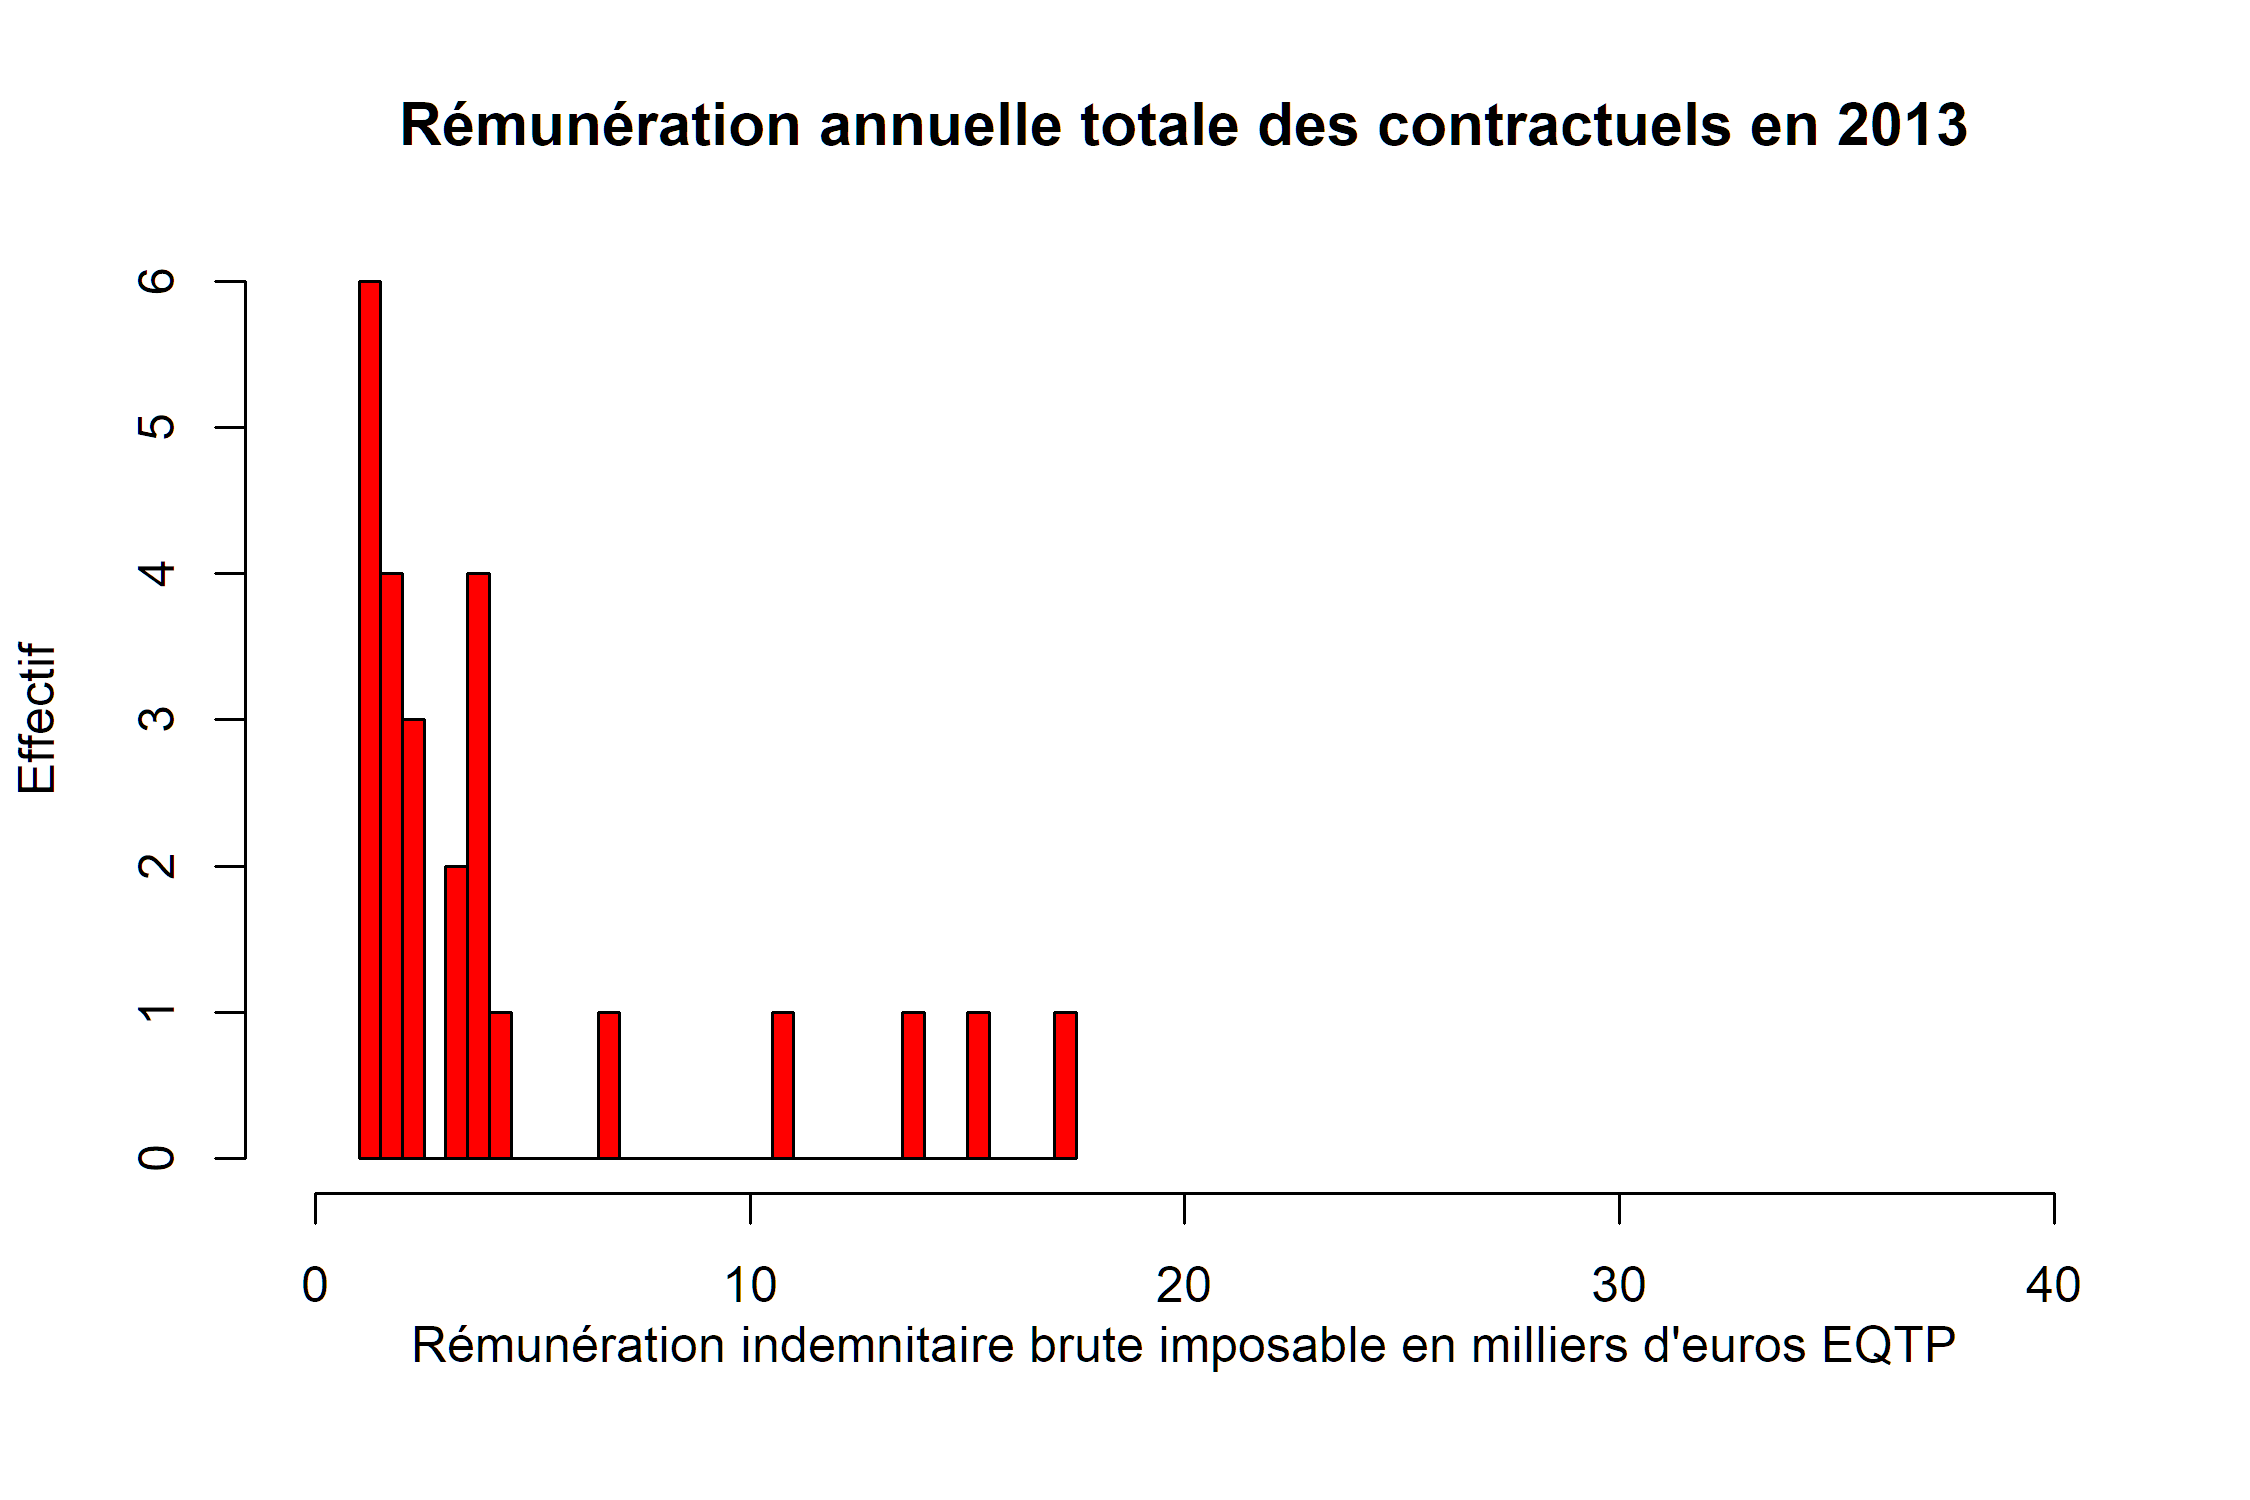
\includegraphics{altair_files/figure-latex/unnamed-chunk-94-1.png}

\textbf{Nota :} Ne sont retenues que les rémunérations supérieures à 1
000 k€. Les élus ne sont pas pris en compte.

\textbf{Formation et distribution du salaire brut moyen par tête (SMPT)
en EQTP pour l'année 2013 }

~\emph{Tableau 3.3.1}

\begin{longtable}[]{@{}rrrrr@{}}
\toprule
Statistique & Primes & Autres rémunérations & Quotité &
Effectif\tabularnewline
\midrule
\endhead
Minimum & -22 & 0 & 0,25 &\tabularnewline
1er quartile & 0 & 0 & 0,5 &\tabularnewline
Médiane & 495 & 0 & 0,71 &\tabularnewline
Moyenne & 2 023 & 0 & 0,71 & 82\tabularnewline
3ème quartile & 1 986 & 0 & 1 &\tabularnewline
Maximum & 17 494 & 0 & 1 &\tabularnewline
\bottomrule
\end{longtable}

~\emph{Tableau 3.3.2}

\begin{longtable}[]{@{}rrrrr@{}}
\toprule
Statistique & Total rémunérations & Total rémunérations EQTP & Quotité &
Effectif\tabularnewline
\midrule
\endhead
Minimum & 4 211 & 4 806 & 0,25 &\tabularnewline
1er quartile & 8 926 & 11 077 & 0,5 &\tabularnewline
Médiane & 12 419 & 16 251 & 0,71 &\tabularnewline
Moyenne & 15 493 & 17 917 & 0,71 & 82\tabularnewline
3ème quartile & 17 776 & 20 174 & 1 &\tabularnewline
Maximum & 58 944 & 58 944 & 1 &\tabularnewline
\bottomrule
\end{longtable}

\href{Bases/Remunerations/Analyse.remunerations.csv}{Lien vers la base
des rémunérations}

\newpage

\hypertarget{remunerations-brutes-par-grade-et-par-emploi}{%
\subsection{3.4 Rémunérations brutes par grade et par
emploi}\label{remunerations-brutes-par-grade-et-par-emploi}}

\href{Bases/Remunerations/brut.eqtp.csv}{Rémunérations brutes par grade}

\href{Bases/Remunerations/brut.eqtp.emploi.csv}{Rémunérations brutes par
emploi}

\hypertarget{comparaisons-source-inseedgcl}{%
\subsection{3.5 Comparaisons source
INSEE/DGCL}\label{comparaisons-source-inseedgcl}}

\emph{Salaires annnuels bruts moyens 2011-2017 en EQTP (hors assistantes
maternelles)}

~\emph{Tableau 3.5.1}

\begin{longtable}[]{@{}llllllll@{}}
\toprule
Agrégat (euros) & 2011 & 2012 & 2013 & 2014 & 2015 & 2016 &
2017\tabularnewline
\midrule
\endhead
Ensemble & 25 908 & 26 340 & 26 616 & 26 844 & 27 384 & 27 636 & 28
356\tabularnewline
Titulaires & 26 676 & 27 108 & 27 444 & 28 044 & 28 464 & 28 764 & 29
472\tabularnewline
Autres salariés* & 22 836 & NA & 24 360 & 24 504 & 24 696 & 24 828 & 25
320\tabularnewline
\bottomrule
\end{longtable}

\begin{itemize}
\tightlist
\item
  \emph{Contractuels à partir de 2017} *
\end{itemize}

\textbf{Eléments de la rémunération brute pour les titulaires de la
fonction publique territoriale}

~\emph{Tableau 3.5.2}

\begin{longtable}[]{@{}lllllll@{}}
\toprule
Rém. annuelles & 2011 & Primes & 2012 & Primes & 2013 &
Primes\tabularnewline
\midrule
\endhead
Salaire brut & 26 660 & & 27 108 & & 27 444 &\tabularnewline
Traitement brut & 20 562 & 22,9 \% & 20 724 & 23,6 \% & 21 060 & 23,6
\%\tabularnewline
Primes et rémunérations annexes & & & & & &\tabularnewline
y compris IR et SFT & 6 098 & & 6 384 & & 6 384 &\tabularnewline
\bottomrule
\end{longtable}

\begin{longtable}[]{@{}lllllll@{}}
\toprule
Rém. annuelles & 2014 & Primes & 2015 & Primes & 2016 &
Primes\tabularnewline
\midrule
\endhead
Salaire brut & 28 044 & & 28 464 & & 28 764 &\tabularnewline
Traitement brut & 21 456 & 23,5 \% & 21 816 & 23,4 \% & 22 104 & 23,2
\%\tabularnewline
Primes et rémunérations annexes & & & & & &\tabularnewline
y compris IR et SFT & 6 588 & & 6 648 & & 6 660 &\tabularnewline
\bottomrule
\end{longtable}

\emph{Champ : France. Salariés en équivalent-temps plein (EQTP) des
collectivités territoriales (y compris bénéficiaires de contrats aidés,
hors assistantes maternelles).}\\
\emph{Les primes sont cumulées au supplément familial de traitement
(SFT) et à l'indemnité de résidence (IR). Le cumul est rapporté à la
rémunération brute totale.}\\
\href{Docs/ip1486.xls}{Source INSEE}\\
\href{Docs/Vue3_Remuneration_2017.xlsx}{Source DGCL}\\
\href{Docs/Vue-Remunerations-2018.xlsx}{Source DGCL}\\
\href{Docs/RA_2015.pdf}{Source RAEFP 2015}\\
\href{Docs/RA_2016.pdf}{Source RAEFP 2016}\\
\href{Docs/RA_2017.pdf}{Source RAEFP 2017}\\
\href{Docs/RA_2018.pdf}{Source RAEFP 2018}

\hypertarget{cout-charge}{%
\subsection{3.6 Coût chargé}\label{cout-charge}}

\textbf{Les liens ci-après renvoient vers des tableaux présentant le
coût moyen chargé par agent}

\href{Bases/Remunerations/cout.eqtp.csv}{Coût moyen chargé par grade}

\href{Bases/Remunerations/cout.eqtp.emploi.csv}{Coût moyen chargé par
emploi}

\hypertarget{remunerations-nettes-evolutions-sur-la-periode-sous-revue}{%
\section{4. Rémunérations nettes : évolutions sur la periode sous
revue}\label{remunerations-nettes-evolutions-sur-la-periode-sous-revue}}

\textbf{Nombre d'exercices: 5 }

\textbf{Périmètre des données}\\
\textbf{Les données présentées dans cette section sont toutes relatives
à des rémunérations nettes en équivalent temps plein (EQTP)}\\
\textbf{Les élus, les vacataires et les assistantes maternelles ont été
retirés de la population étudiée}\\
\textbf{Seuls sont considérés les postes actifs et non annexes}

\emph{Nota :}\\
\emph{Rémunération annualisée en EQTP (Equivalent temps plein) : la
rémunération annuelle équivalente pour un temps plein en année pleine
est calculée pour chaque agent}\\
\emph{Chaque agent est rentre ensuite dans la somme avec la pondération
correspondant à son temps de travail annuel. }

\hypertarget{distribution-de-la-remuneration-nette-moyenne-sur-la-periode}{%
\subsection{4.1 Distribution de la rémunération nette moyenne sur la
periode}\label{distribution-de-la-remuneration-nette-moyenne-sur-la-periode}}

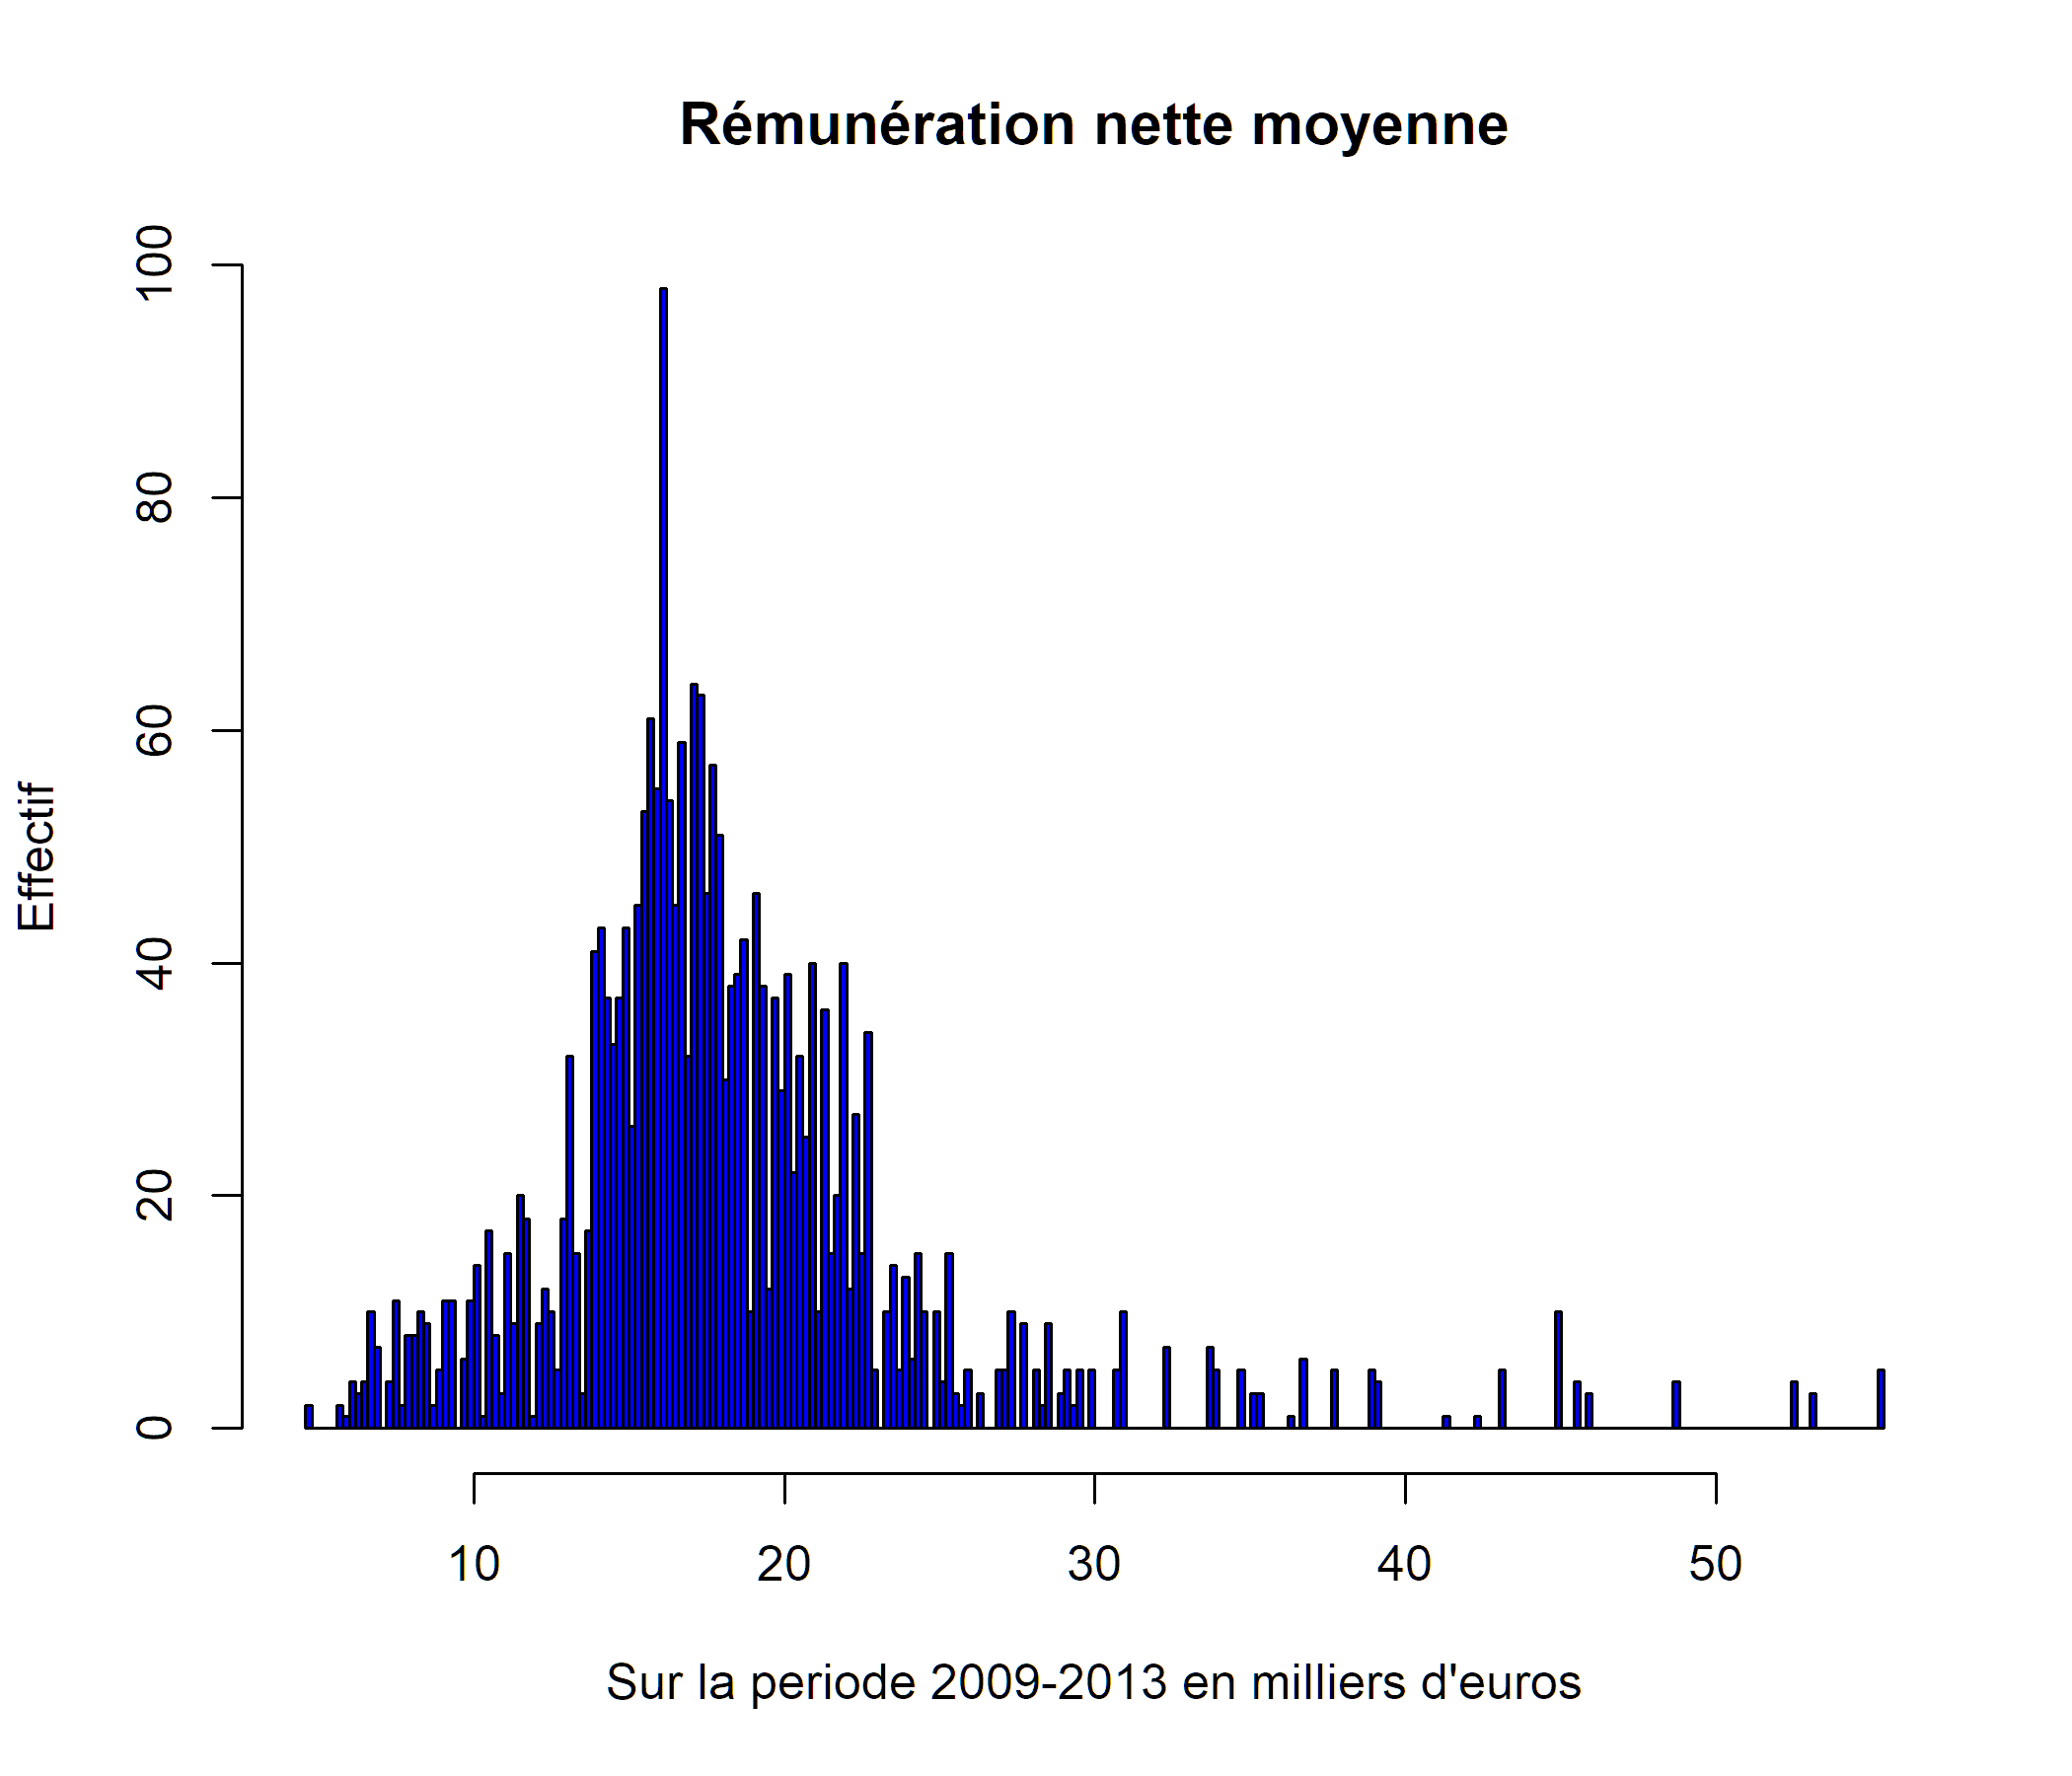
\includegraphics{altair_files/figure-latex/unnamed-chunk-115-1.png}

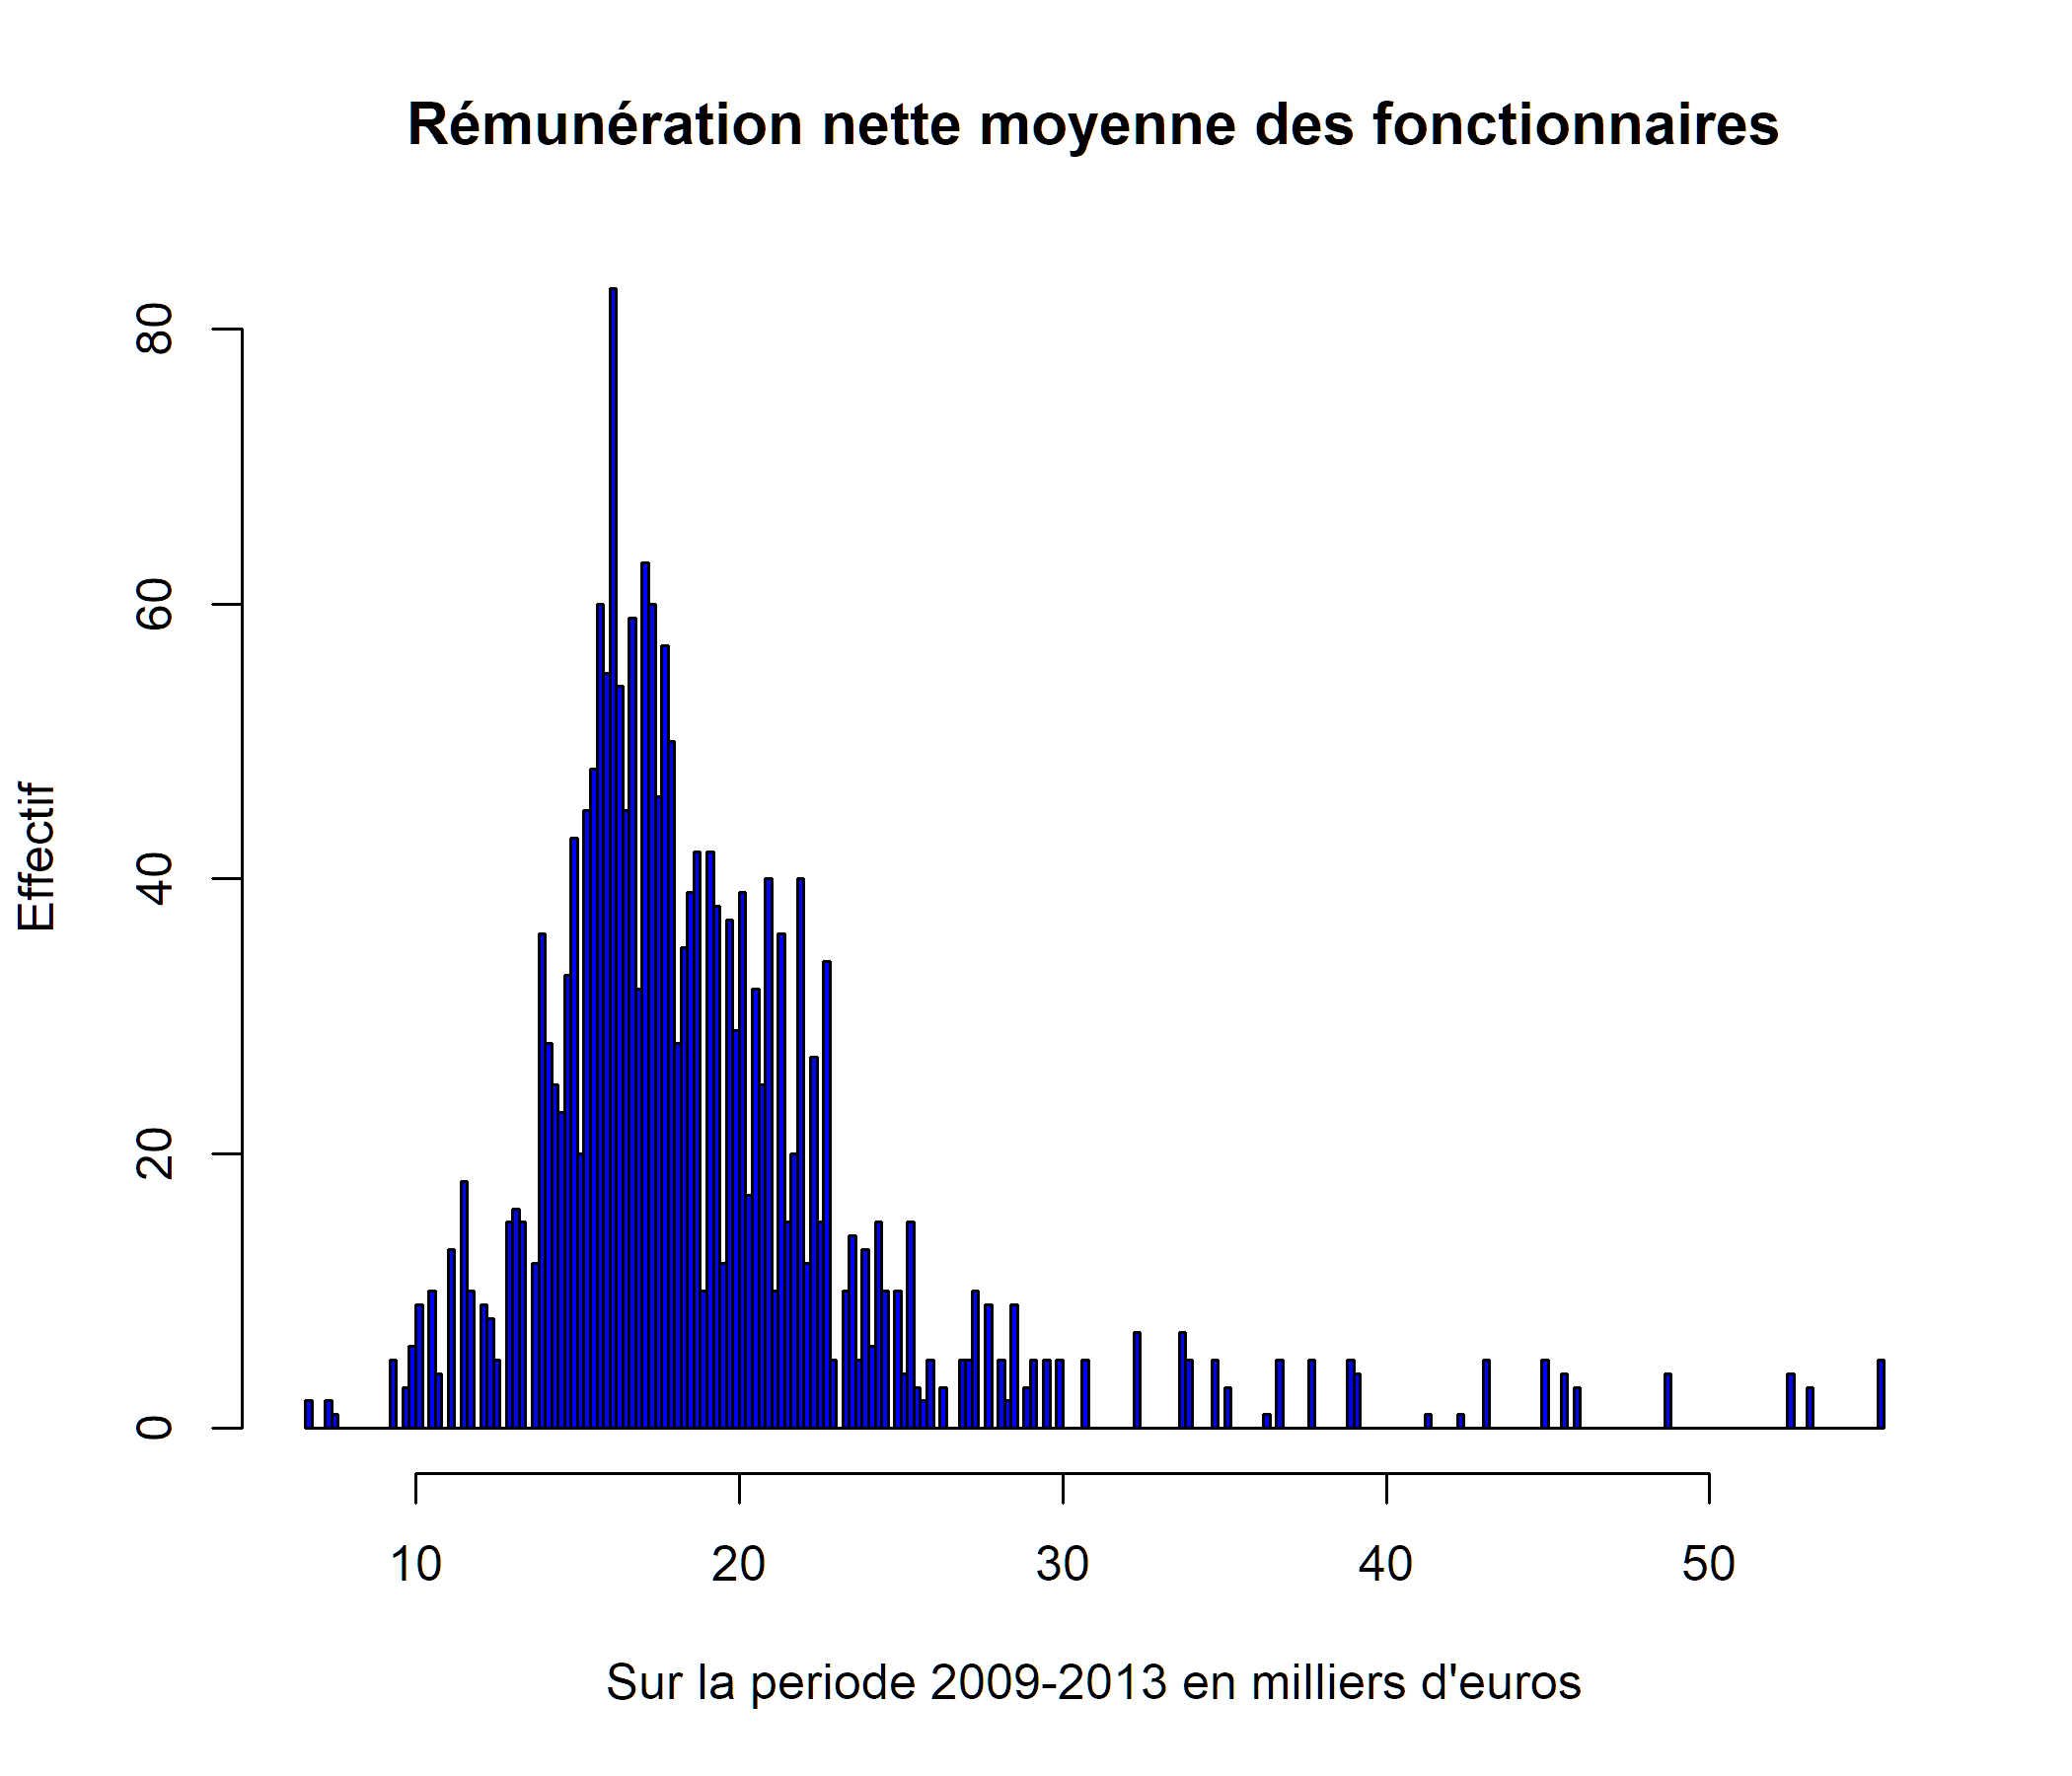
\includegraphics{altair_files/figure-latex/unnamed-chunk-116-1.png}

\href{Bases/Remunerations/Analyse.variations.csv}{Lien vers la base de
données synthétique}\\
\href{Bases/Remunerations/Analyse.variations.par.exercice.csv}{Lien vers
la base de données détaillée par année}

\hypertarget{evolutions-du-smpt-sur-la-periode-sous-revue}{%
\subsection{4.2 Evolutions du SMPT sur la periode sous
revue}\label{evolutions-du-smpt-sur-la-periode-sous-revue}}

\hypertarget{evolution-du-smpt-pour-lensemble-des-personnels-fonctionnaires-et-non-titulaires-hors-elus}{%
\subsubsection{4.2.1 Evolution du SMPT pour l'ensemble des personnels
fonctionnaires et non titulaires (hors
élus)}\label{evolution-du-smpt-pour-lensemble-des-personnels-fonctionnaires-et-non-titulaires-hors-elus}}

\textbf{Salaire net moyen par tête (SMPT net) en EQTP, hors élus}

~\emph{Tableau 4.2.1.1}

\begin{longtable}[]{@{}ccccc@{}}
\toprule
\begin{minipage}[b]{0.07\columnwidth}\centering
Annee\strut
\end{minipage} & \begin{minipage}[b]{0.18\columnwidth}\centering
smpt net (euros)\strut
\end{minipage} & \begin{minipage}[b]{0.15\columnwidth}\centering
Variation (\%)\strut
\end{minipage} & \begin{minipage}[b]{0.32\columnwidth}\centering
smpt net temps complet (euros)\strut
\end{minipage} & \begin{minipage}[b]{0.15\columnwidth}\centering
Variation (\%)\strut
\end{minipage}\tabularnewline
\midrule
\endhead
\begin{minipage}[t]{0.07\columnwidth}\centering
2009\strut
\end{minipage} & \begin{minipage}[t]{0.18\columnwidth}\centering
18 548\strut
\end{minipage} & \begin{minipage}[t]{0.15\columnwidth}\centering
\strut
\end{minipage} & \begin{minipage}[t]{0.32\columnwidth}\centering
19 565\strut
\end{minipage} & \begin{minipage}[t]{0.15\columnwidth}\centering
\strut
\end{minipage}\tabularnewline
\begin{minipage}[t]{0.07\columnwidth}\centering
2010\strut
\end{minipage} & \begin{minipage}[t]{0.18\columnwidth}\centering
18 564\strut
\end{minipage} & \begin{minipage}[t]{0.15\columnwidth}\centering
\strut
\end{minipage} & \begin{minipage}[t]{0.32\columnwidth}\centering
19 870\strut
\end{minipage} & \begin{minipage}[t]{0.15\columnwidth}\centering
\strut
\end{minipage}\tabularnewline
\begin{minipage}[t]{0.07\columnwidth}\centering
2011\strut
\end{minipage} & \begin{minipage}[t]{0.18\columnwidth}\centering
18 698\strut
\end{minipage} & \begin{minipage}[t]{0.15\columnwidth}\centering
4,18\strut
\end{minipage} & \begin{minipage}[t]{0.32\columnwidth}\centering
20 155\strut
\end{minipage} & \begin{minipage}[t]{0.15\columnwidth}\centering
9,09\strut
\end{minipage}\tabularnewline
\begin{minipage}[t]{0.07\columnwidth}\centering
2012\strut
\end{minipage} & \begin{minipage}[t]{0.18\columnwidth}\centering
18 933\strut
\end{minipage} & \begin{minipage}[t]{0.15\columnwidth}\centering
\strut
\end{minipage} & \begin{minipage}[t]{0.32\columnwidth}\centering
20 869\strut
\end{minipage} & \begin{minipage}[t]{0.15\columnwidth}\centering
\strut
\end{minipage}\tabularnewline
\begin{minipage}[t]{0.07\columnwidth}\centering
2013\strut
\end{minipage} & \begin{minipage}[t]{0.18\columnwidth}\centering
19 324\strut
\end{minipage} & \begin{minipage}[t]{0.15\columnwidth}\centering
\strut
\end{minipage} & \begin{minipage}[t]{0.32\columnwidth}\centering
21 343\strut
\end{minipage} & \begin{minipage}[t]{0.15\columnwidth}\centering
\strut
\end{minipage}\tabularnewline
\bottomrule
\end{longtable}

\textbf{Distribution et variation sur la periode du salaire moyen net
par tête (SMPT net) en EQTP}\\
\textbf{pour les salariés à temps complet}

~\emph{Tableau 4.2.1.2}

\begin{longtable}[]{@{}rrrrrrrrr@{}}
\toprule
Statistique & 2009 & Effectif & 2009 TC & Effectif & 2013 & Effectif &
2013 TC & Effectif\tabularnewline
\midrule
\endhead
Minimum & 6 172 & & 13 922 & & 4 794 & & 4 794 &\tabularnewline
1er quartile & 15 338 & & 16 047 & & 16 580 & & 17 624 &\tabularnewline
Médiane & 17 019 & & 17 882 & & 18 237 & & 19 820 &\tabularnewline
Moyenne & 18 548 & 476 & 19 565 & 246 & 19 324 & 477 & 21 343 &
237\tabularnewline
3ème quartile & 20 215 & & 20 913 & & 21 609 & & 23 114 &\tabularnewline
Maximum & 56 154 & & 56 154 & & 54 534 & & 54 534 &\tabularnewline
\bottomrule
\end{longtable}

\emph{Nota :} La population retenue est constituée des agents qui ne
font pas partie des 2 centiles extrêmaux

Les élus, vacataires et assistantes maternelles sont retirés du
périmètre.\\
TC : personnels à temps complet sur toute l'annee\\
Seuls sont pris en compte les agents ayant connu au moins un mois actif
et ayant eu, sur l'annee, des rémunérations non annexes.\\
\href{Docs/méthodologie.pdf}{Compléments méthodologiques}

\textbf{Comparaisons source INSEE/DGCL}

\textbf{Salaires nets annuels moyens en EQTP (hors assistantes
maternelles) dans la FPT}

~\emph{Tableau 4.2.1.3}

\begin{longtable}[]{@{}lrrrrrr@{}}
\toprule
net (euros) & 2011 & 2012 & 2013 & 2014 & 2016 & 2017\tabularnewline
\midrule
\endhead
Ensemble & 21 876 & 22 176 & 22 224 & 22 524 & 22 824 & 23
328\tabularnewline
Titulaires & 22 632 & 22 920 & 22 920 & 23 424 & 23 820 & 24
312\tabularnewline
Autres salariés* & 18 864 & NA & NA & 18 732 & 20 207 & 20
532\tabularnewline
\bottomrule
\end{longtable}

*Contractuels à partir de 2017

\emph{Champ : France. Salariés en équivalent-temps plein (EQTP) des
collectivités territoriales (y compris bénéficiaires de contrats aidés,
hors assistantes maternelles).}

\textbf{Distribution des salaires nets annuels en EQTP dans la fonction
publique territoriale (2011-2016)}

~\emph{Tableau 4.2.1.4}

\begin{longtable}[]{@{}llllll@{}}
\toprule
Décile ~euros & 2011 FPT & 2013 FPT & 2014 FPT & 2016 FPT & 2017
FPT\tabularnewline
\midrule
\endhead
D1 & 15 288 & 15 600 & 15 768 & 15 912 & 16 272\tabularnewline
D2 & 16 512 & 16 860 & 17 124 & 17 340 & 17 688\tabularnewline
D3 & 17 508 & 17 844 & 18 156 & 18 432 & 18 828\tabularnewline
D4 & 18 480 & 18 816 & 19 164 & 19 476 & 19 908\tabularnewline
D5 (médiane) & 19 632 & 19 908 & 20 256 & 20 616 & 21 096\tabularnewline
D6 & 21 012 & 21 300 & 21 648 & 22 020 & 22 548\tabularnewline
D7 & 22 860 & 23 160 & 23 496 & 23 868 & 24 444\tabularnewline
D8 & 25 596 & 25 956 & 26 292 & 26 700 & 27 336\tabularnewline
D9 & 30 876 & 31 272 & 31 596 & 31 968 & 32 652\tabularnewline
Moyenne & 21 876 & 22 212 & 22 524 & 22 824 & 23 328\tabularnewline
\bottomrule
\end{longtable}

\textbf{Distribution des salaires nets annuels en EQTP dans la fonction
publique d'Etat (2011-2016)}

~\emph{Tableau 4.2.1.5}

\begin{longtable}[]{@{}llll@{}}
\toprule
Décile ~euros & 2011 & 2013 & 2016\tabularnewline
\midrule
\endhead
D1 & 17 496 & 18 012 & 17 928\tabularnewline
D2 & 20 916 & 21 348 & 21 588\tabularnewline
D3 & 23 052 & 23 376 & 23 844\tabularnewline
D4 & 24 912 & 25 248 & 25 764\tabularnewline
D5 (médiane) & 26 832 & 27 120 & 27 720\tabularnewline
D6 & 28 944 & 29 220 & 29 760\tabularnewline
D7 & 31 632 & 31 968 & 32 604\tabularnewline
D8 & 35 592 & 35 964 & 36 588\tabularnewline
D9 & 42 456 & 42 780 & 43 332\tabularnewline
Moyenne & 29 208 & 29 628 & 30 060\tabularnewline
\bottomrule
\end{longtable}

\textbf{Distribution des salaires nets annuels en EQTP dans la fonction
publique hospitalière (hôpitaux) (2011-2016)}

~\emph{Tableau 4.2.1.6}

\begin{longtable}[]{@{}lllll@{}}
\toprule
Décile ~euros & 2011 & 2013 & 2016 & 2017\tabularnewline
\midrule
\endhead
D1 & 16 584 & 17 016 & 17 460 & 17 688\tabularnewline
D2 & 18 168 & 18 492 & 18 852 & 19 104\tabularnewline
D3 & 19 620 & 19 872 & 20 160 & 20 460\tabularnewline
D4 & 21 048 & 21 192 & 21 456 & 21 816\tabularnewline
D5 (médiane) & 22 596 & 22 656 & 22 848 & 23 220\tabularnewline
D6 & 24 504 & 24 516 & 24 540 & 24 888\tabularnewline
D7 & 27 216 & 27 252 & 27 108 & 27 408\tabularnewline
D8 & 30 996 & 31 176 & 31 092 & 31 404\tabularnewline
D9 & 37 812 & 38 100 & 38 064 & 38 388\tabularnewline
Moyenne & 26 496 & 26 916 & 27 096 & 27 456\tabularnewline
\bottomrule
\end{longtable}

\href{Docs/ip1486.xls}{Source INSEE, onglets Figure3, F1web et F3web -
2011}\\
\href{Docs/vue3_remunerations.xls}{Source INSEE, onglets F V3.1-2, F
V3.1-5 - 2013}\\
\href{Docs/Vue-Remunerations-2018.xlsx}{Source INSEE, onglet v3-2, V3-5
2016}

\hypertarget{evolution-du-smpt-des-fonctionnaires}{%
\subsubsection{4.2.2 Evolution du SMPT des
fonctionnaires}\label{evolution-du-smpt-des-fonctionnaires}}

\hypertarget{toutes-categories-statutaires}{%
\subparagraph{4.2.2.1 Toutes categories
statutaires}\label{toutes-categories-statutaires}}

\textbf{Salaire net moyen par tête (SMPT net) en EQTP}

~\emph{Tableau 4.2.2.1.1}

\begin{longtable}[]{@{}ccccc@{}}
\toprule
\begin{minipage}[b]{0.07\columnwidth}\centering
Annee\strut
\end{minipage} & \begin{minipage}[b]{0.18\columnwidth}\centering
smpt net (euros)\strut
\end{minipage} & \begin{minipage}[b]{0.15\columnwidth}\centering
Variation (\%)\strut
\end{minipage} & \begin{minipage}[b]{0.32\columnwidth}\centering
smpt net temps complet (euros)\strut
\end{minipage} & \begin{minipage}[b]{0.15\columnwidth}\centering
Variation (\%)\strut
\end{minipage}\tabularnewline
\midrule
\endhead
\begin{minipage}[t]{0.07\columnwidth}\centering
2009\strut
\end{minipage} & \begin{minipage}[t]{0.18\columnwidth}\centering
18 903\strut
\end{minipage} & \begin{minipage}[t]{0.15\columnwidth}\centering
\strut
\end{minipage} & \begin{minipage}[t]{0.32\columnwidth}\centering
19 454\strut
\end{minipage} & \begin{minipage}[t]{0.15\columnwidth}\centering
\strut
\end{minipage}\tabularnewline
\begin{minipage}[t]{0.07\columnwidth}\centering
2010\strut
\end{minipage} & \begin{minipage}[t]{0.18\columnwidth}\centering
18 952\strut
\end{minipage} & \begin{minipage}[t]{0.15\columnwidth}\centering
\strut
\end{minipage} & \begin{minipage}[t]{0.32\columnwidth}\centering
19 730\strut
\end{minipage} & \begin{minipage}[t]{0.15\columnwidth}\centering
\strut
\end{minipage}\tabularnewline
\begin{minipage}[t]{0.07\columnwidth}\centering
2011\strut
\end{minipage} & \begin{minipage}[t]{0.18\columnwidth}\centering
19 158\strut
\end{minipage} & \begin{minipage}[t]{0.15\columnwidth}\centering
5,5\strut
\end{minipage} & \begin{minipage}[t]{0.32\columnwidth}\centering
20 044\strut
\end{minipage} & \begin{minipage}[t]{0.15\columnwidth}\centering
9,21\strut
\end{minipage}\tabularnewline
\begin{minipage}[t]{0.07\columnwidth}\centering
2012\strut
\end{minipage} & \begin{minipage}[t]{0.18\columnwidth}\centering
19 509\strut
\end{minipage} & \begin{minipage}[t]{0.15\columnwidth}\centering
\strut
\end{minipage} & \begin{minipage}[t]{0.32\columnwidth}\centering
20 708\strut
\end{minipage} & \begin{minipage}[t]{0.15\columnwidth}\centering
\strut
\end{minipage}\tabularnewline
\begin{minipage}[t]{0.07\columnwidth}\centering
2013\strut
\end{minipage} & \begin{minipage}[t]{0.18\columnwidth}\centering
19 943\strut
\end{minipage} & \begin{minipage}[t]{0.15\columnwidth}\centering
\strut
\end{minipage} & \begin{minipage}[t]{0.32\columnwidth}\centering
21 245\strut
\end{minipage} & \begin{minipage}[t]{0.15\columnwidth}\centering
\strut
\end{minipage}\tabularnewline
\bottomrule
\end{longtable}

\hypertarget{par-categorie-statutaire}{%
\subparagraph{4.2.2.2 Par categorie
statutaire}\label{par-categorie-statutaire}}

\textbf{Categorie A}

~\emph{Tableau 4.2.2.2.1}

\begin{longtable}[]{@{}ccccc@{}}
\toprule
\begin{minipage}[b]{0.07\columnwidth}\centering
Annee\strut
\end{minipage} & \begin{minipage}[b]{0.18\columnwidth}\centering
smpt net (euros)\strut
\end{minipage} & \begin{minipage}[b]{0.15\columnwidth}\centering
Variation (\%)\strut
\end{minipage} & \begin{minipage}[b]{0.32\columnwidth}\centering
smpt net temps complet (euros)\strut
\end{minipage} & \begin{minipage}[b]{0.15\columnwidth}\centering
Variation (\%)\strut
\end{minipage}\tabularnewline
\midrule
\endhead
\begin{minipage}[t]{0.07\columnwidth}\centering
2009\strut
\end{minipage} & \begin{minipage}[t]{0.18\columnwidth}\centering
38 873\strut
\end{minipage} & \begin{minipage}[t]{0.15\columnwidth}\centering
\strut
\end{minipage} & \begin{minipage}[t]{0.32\columnwidth}\centering
36 699\strut
\end{minipage} & \begin{minipage}[t]{0.15\columnwidth}\centering
\strut
\end{minipage}\tabularnewline
\begin{minipage}[t]{0.07\columnwidth}\centering
2010\strut
\end{minipage} & \begin{minipage}[t]{0.18\columnwidth}\centering
38 080\strut
\end{minipage} & \begin{minipage}[t]{0.15\columnwidth}\centering
\strut
\end{minipage} & \begin{minipage}[t]{0.32\columnwidth}\centering
36 440\strut
\end{minipage} & \begin{minipage}[t]{0.15\columnwidth}\centering
\strut
\end{minipage}\tabularnewline
\begin{minipage}[t]{0.07\columnwidth}\centering
2011\strut
\end{minipage} & \begin{minipage}[t]{0.18\columnwidth}\centering
37 960\strut
\end{minipage} & \begin{minipage}[t]{0.15\columnwidth}\centering
-11,1\strut
\end{minipage} & \begin{minipage}[t]{0.32\columnwidth}\centering
36 643\strut
\end{minipage} & \begin{minipage}[t]{0.15\columnwidth}\centering
1,57\strut
\end{minipage}\tabularnewline
\begin{minipage}[t]{0.07\columnwidth}\centering
2012\strut
\end{minipage} & \begin{minipage}[t]{0.18\columnwidth}\centering
35 970\strut
\end{minipage} & \begin{minipage}[t]{0.15\columnwidth}\centering
\strut
\end{minipage} & \begin{minipage}[t]{0.32\columnwidth}\centering
36 788\strut
\end{minipage} & \begin{minipage}[t]{0.15\columnwidth}\centering
\strut
\end{minipage}\tabularnewline
\begin{minipage}[t]{0.07\columnwidth}\centering
2013\strut
\end{minipage} & \begin{minipage}[t]{0.18\columnwidth}\centering
34 574\strut
\end{minipage} & \begin{minipage}[t]{0.15\columnwidth}\centering
\strut
\end{minipage} & \begin{minipage}[t]{0.32\columnwidth}\centering
37 276\strut
\end{minipage} & \begin{minipage}[t]{0.15\columnwidth}\centering
\strut
\end{minipage}\tabularnewline
\bottomrule
\end{longtable}

\emph{Comparaisons nationales}\\
\emph{FPT categorie A}

\begin{longtable}[]{@{}lllll@{}}
\toprule
Décile ~euros & 2011 & 2013 & 2014 & 2016\tabularnewline
\midrule
\endhead
D1 & 26 040 & 26 340 & 26 460 & 26 724\tabularnewline
D2 & 28 992 & & &\tabularnewline
D3 & 31 272 & & &\tabularnewline
D4 & 33 468 & & &\tabularnewline
D5 (médiane) & 35 820 & 36 312 & 36 580 & 37 020\tabularnewline
D6 & 38 664 & & &\tabularnewline
D7 & 42 276 & & &\tabularnewline
D8 & 47 124 & & &\tabularnewline
D9 & 54 840 & 55 032 & 55 440 & 55 284\tabularnewline
Moyenne & 38 700 & 39 120 & 39 360 & 39 564\tabularnewline
\bottomrule
\end{longtable}

\textbf{Categorie B}

~\emph{Tableau 4.2.2.2.2}

\begin{longtable}[]{@{}ccccc@{}}
\toprule
\begin{minipage}[b]{0.07\columnwidth}\centering
Annee\strut
\end{minipage} & \begin{minipage}[b]{0.18\columnwidth}\centering
smpt net (euros)\strut
\end{minipage} & \begin{minipage}[b]{0.15\columnwidth}\centering
Variation (\%)\strut
\end{minipage} & \begin{minipage}[b]{0.32\columnwidth}\centering
smpt net temps complet (euros)\strut
\end{minipage} & \begin{minipage}[b]{0.15\columnwidth}\centering
Variation (\%)\strut
\end{minipage}\tabularnewline
\midrule
\endhead
\begin{minipage}[t]{0.07\columnwidth}\centering
2009\strut
\end{minipage} & \begin{minipage}[t]{0.18\columnwidth}\centering
23 324\strut
\end{minipage} & \begin{minipage}[t]{0.15\columnwidth}\centering
\strut
\end{minipage} & \begin{minipage}[t]{0.32\columnwidth}\centering
24 328\strut
\end{minipage} & \begin{minipage}[t]{0.15\columnwidth}\centering
\strut
\end{minipage}\tabularnewline
\begin{minipage}[t]{0.07\columnwidth}\centering
2010\strut
\end{minipage} & \begin{minipage}[t]{0.18\columnwidth}\centering
23 168\strut
\end{minipage} & \begin{minipage}[t]{0.15\columnwidth}\centering
\strut
\end{minipage} & \begin{minipage}[t]{0.32\columnwidth}\centering
24 309\strut
\end{minipage} & \begin{minipage}[t]{0.15\columnwidth}\centering
\strut
\end{minipage}\tabularnewline
\begin{minipage}[t]{0.07\columnwidth}\centering
2011\strut
\end{minipage} & \begin{minipage}[t]{0.18\columnwidth}\centering
23 044\strut
\end{minipage} & \begin{minipage}[t]{0.15\columnwidth}\centering
2,6\strut
\end{minipage} & \begin{minipage}[t]{0.32\columnwidth}\centering
24 467\strut
\end{minipage} & \begin{minipage}[t]{0.15\columnwidth}\centering
4,96\strut
\end{minipage}\tabularnewline
\begin{minipage}[t]{0.07\columnwidth}\centering
2012\strut
\end{minipage} & \begin{minipage}[t]{0.18\columnwidth}\centering
22 773\strut
\end{minipage} & \begin{minipage}[t]{0.15\columnwidth}\centering
\strut
\end{minipage} & \begin{minipage}[t]{0.32\columnwidth}\centering
24 144\strut
\end{minipage} & \begin{minipage}[t]{0.15\columnwidth}\centering
\strut
\end{minipage}\tabularnewline
\begin{minipage}[t]{0.07\columnwidth}\centering
2013\strut
\end{minipage} & \begin{minipage}[t]{0.18\columnwidth}\centering
23 931\strut
\end{minipage} & \begin{minipage}[t]{0.15\columnwidth}\centering
\strut
\end{minipage} & \begin{minipage}[t]{0.32\columnwidth}\centering
25 535\strut
\end{minipage} & \begin{minipage}[t]{0.15\columnwidth}\centering
\strut
\end{minipage}\tabularnewline
\bottomrule
\end{longtable}

\emph{Comparaisons nationales}\\
\emph{FPT categorie B}

\begin{longtable}[]{@{}lllll@{}}
\toprule
Décile ~euros & 2011 & 2013 & 2014 & 2016\tabularnewline
\midrule
\endhead
D1 & 20 580 & 20 964 & 21 108 & 21 372\tabularnewline
D2 & 22 272 & & &\tabularnewline
D3 & 23 652 & & &\tabularnewline
D4 & 24 960 & & &\tabularnewline
D5 (médiane) & 26 244 & 26 820 & 27 000 & 27 216\tabularnewline
D6 & 27 636 & & &\tabularnewline
D7 & 29 160 & & &\tabularnewline
D8 & 30 984 & & &\tabularnewline
D9 & 33 804 & 34 224 & 34 344 & 34 560\tabularnewline
Moyenne & 26 940 & 27 408 & 27 588 & 27 828\tabularnewline
\bottomrule
\end{longtable}

\textbf{Categorie C}

~\emph{Tableau 4.2.2.2.3}

\begin{longtable}[]{@{}ccccc@{}}
\toprule
\begin{minipage}[b]{0.07\columnwidth}\centering
Annee\strut
\end{minipage} & \begin{minipage}[b]{0.18\columnwidth}\centering
smpt net (euros)\strut
\end{minipage} & \begin{minipage}[b]{0.15\columnwidth}\centering
Variation (\%)\strut
\end{minipage} & \begin{minipage}[b]{0.32\columnwidth}\centering
smpt net temps complet (euros)\strut
\end{minipage} & \begin{minipage}[b]{0.15\columnwidth}\centering
Variation (\%)\strut
\end{minipage}\tabularnewline
\midrule
\endhead
\begin{minipage}[t]{0.07\columnwidth}\centering
2009\strut
\end{minipage} & \begin{minipage}[t]{0.18\columnwidth}\centering
16 877\strut
\end{minipage} & \begin{minipage}[t]{0.15\columnwidth}\centering
\strut
\end{minipage} & \begin{minipage}[t]{0.32\columnwidth}\centering
17 731\strut
\end{minipage} & \begin{minipage}[t]{0.15\columnwidth}\centering
\strut
\end{minipage}\tabularnewline
\begin{minipage}[t]{0.07\columnwidth}\centering
2010\strut
\end{minipage} & \begin{minipage}[t]{0.18\columnwidth}\centering
17 008\strut
\end{minipage} & \begin{minipage}[t]{0.15\columnwidth}\centering
\strut
\end{minipage} & \begin{minipage}[t]{0.32\columnwidth}\centering
17 963\strut
\end{minipage} & \begin{minipage}[t]{0.15\columnwidth}\centering
\strut
\end{minipage}\tabularnewline
\begin{minipage}[t]{0.07\columnwidth}\centering
2011\strut
\end{minipage} & \begin{minipage}[t]{0.18\columnwidth}\centering
17 155\strut
\end{minipage} & \begin{minipage}[t]{0.15\columnwidth}\centering
8,89\strut
\end{minipage} & \begin{minipage}[t]{0.32\columnwidth}\centering
18 168\strut
\end{minipage} & \begin{minipage}[t]{0.15\columnwidth}\centering
8,58\strut
\end{minipage}\tabularnewline
\begin{minipage}[t]{0.07\columnwidth}\centering
2012\strut
\end{minipage} & \begin{minipage}[t]{0.18\columnwidth}\centering
17 916\strut
\end{minipage} & \begin{minipage}[t]{0.15\columnwidth}\centering
\strut
\end{minipage} & \begin{minipage}[t]{0.32\columnwidth}\centering
18 902\strut
\end{minipage} & \begin{minipage}[t]{0.15\columnwidth}\centering
\strut
\end{minipage}\tabularnewline
\begin{minipage}[t]{0.07\columnwidth}\centering
2013\strut
\end{minipage} & \begin{minipage}[t]{0.18\columnwidth}\centering
18 378\strut
\end{minipage} & \begin{minipage}[t]{0.15\columnwidth}\centering
\strut
\end{minipage} & \begin{minipage}[t]{0.32\columnwidth}\centering
19 252\strut
\end{minipage} & \begin{minipage}[t]{0.15\columnwidth}\centering
\strut
\end{minipage}\tabularnewline
\bottomrule
\end{longtable}

\emph{Comparaisons nationales}\\
\emph{FPT categorie C}

\begin{longtable}[]{@{}lllll@{}}
\toprule
Décile ~euros & 2011 & 2013 & 2014 & 2016\tabularnewline
\midrule
\endhead
D1 & 15 972 & 16 296 & 16 632 & 16 920\tabularnewline
D2 & 16 896 & & &\tabularnewline
D3 & 17 652 & & &\tabularnewline
D4 & 18 360 & & &\tabularnewline
D5 (médiane) & 19 164 & 19 464 & 19 884 & 20 256\tabularnewline
D6 & 20 100 & & &\tabularnewline
D7 & 21 216 & & &\tabularnewline
D8 & 22 680 & & &\tabularnewline
D9 & 24 996 & 25 176 & 25 608 & 26 028\tabularnewline
Moyenne & 20 016 & 20 268 & 20 676 & 21 024\tabularnewline
\bottomrule
\end{longtable}

\hypertarget{distribution-et-variation-sur-la-periode-du-smpt-net-en-eqtp}{%
\subsubsection{4.2.3 Distribution et variation sur la periode du SMPT
net en
EQTP}\label{distribution-et-variation-sur-la-periode-du-smpt-net-en-eqtp}}

\hypertarget{pour-lensemble-des-categories-statutaires}{%
\paragraph{4.2.3.1 Pour l'ensemble des categories
statutaires}\label{pour-lensemble-des-categories-statutaires}}

\textbf{Fonctionnaires}\\
\hspace*{0.333em}\emph{Tableau 4.2.3.1.1}

\begin{longtable}[]{@{}rrrrrrrrr@{}}
\toprule
Statistique & 2009 & Effectif & 2009 TC & Effectif & 2013 & Effectif &
2013 TC & Effectif\tabularnewline
\midrule
\endhead
Minimum & 7 081 & & 13 922 & & 5 741 & & 8 898 &\tabularnewline
1er quartile & 15 640 & & 16 054 & & 16 991 & & 17 631 &\tabularnewline
Médiane & 17 241 & & 17 796 & & 18 859 & & 19 800 &\tabularnewline
Moyenne & 18 903 & 411 & 19 454 & 236 & 19 943 & 395 & 21 245 &
230\tabularnewline
3ème quartile & 20 410 & & 20 737 & & 21 976 & & 23 011 &\tabularnewline
Maximum & 56 154 & & 56 154 & & 54 534 & & 54 534 &\tabularnewline
\bottomrule
\end{longtable}

\hypertarget{par-categorie-statutaire-1}{%
\paragraph{4.2.3.2 Par categorie
statutaire}\label{par-categorie-statutaire-1}}

\textbf{Categorie A}\\
\hspace*{0.333em}\emph{Tableau 4.2.3.2.1}

\begin{longtable}[]{@{}rrrrrrrrr@{}}
\toprule
Statistique & 2009 & Effectif & 2009 TC & Effectif & 2013 & Effectif &
2013 TC & Effectif\tabularnewline
\midrule
\endhead
Minimum & 23 657 & & 23 657 & & 20 433 & & 28 540 &\tabularnewline
1er quartile & 32 165 & & 32 709 & & 28 540 & & 29 829 &\tabularnewline
Médiane & 36 270 & & 36 197 & & 33 089 & & 35 255 &\tabularnewline
Moyenne & 38 873 & 24 & 36 699 & 13 & 34 574 & 18 & 37 276 &
13\tabularnewline
3ème quartile & 45 114 & & 42 346 & & 40 490 & & 41 158 &\tabularnewline
Maximum & 56 154 & & 56 154 & & 54 534 & & 54 534 &\tabularnewline
\bottomrule
\end{longtable}

\textbf{Categorie B}\\
\hspace*{0.333em}\emph{Tableau 4.2.3.2.2}

\begin{longtable}[]{@{}rrrrrrrrr@{}}
\toprule
Statistique & 2009 & Effectif & 2009 TC & Effectif & 2013 & Effectif &
2013 TC & Effectif\tabularnewline
\midrule
\endhead
Minimum & 17 781 & & 19 172 & & 13 409 & & 20 056 &\tabularnewline
1er quartile & 20 810 & & 22 576 & & 21 517 & & 22 424 &\tabularnewline
Médiane & 22 734 & & 23 503 & & 23 500 & & 25 050 &\tabularnewline
Moyenne & 23 324 & 53 & 24 328 & 25 & 23 931 & 61 & 25 535 &
37\tabularnewline
3ème quartile & 25 842 & & 26 105 & & 26 093 & & 26 735 &\tabularnewline
Maximum & 30 876 & & 30 876 & & 35 160 & & 35 160 &\tabularnewline
\bottomrule
\end{longtable}

\textbf{Categorie C}\\
\hspace*{0.333em}\emph{Tableau 4.2.3.2.3}

\begin{longtable}[]{@{}rrrrrrrrr@{}}
\toprule
Statistique & 2009 & Effectif & 2009 TC & Effectif & 2013 & Effectif &
2013 TC & Effectif\tabularnewline
\midrule
\endhead
Minimum & 7 081 & & 13 922 & & 5 741 & & 8 898 &\tabularnewline
1er quartile & 15 429 & & 15 886 & & 16 791 & & 17 346 &\tabularnewline
Médiane & 16 526 & & 17 101 & & 17 916 & & 18 863 &\tabularnewline
Moyenne & 16 877 & 310 & 17 731 & 186 & 18 378 & 293 & 19 252 &
169\tabularnewline
3ème quartile & 18 664 & & 19 248 & & 20 258 & & 21 066 &\tabularnewline
Maximum & 28 668 & & 28 668 & & 31 084 & & 31 084 &\tabularnewline
\bottomrule
\end{longtable}

\href{Bases/Remunerations/Analyse.variations.par.exercice.csv}{Lien vers
la base de données}

\hypertarget{remuneration-moyenne-des-personnes-en-place-rmpp-et-effet-de-noria}{%
\subsection{4.3 Rémunération moyenne des personnes en place (RMPP) et
effet de
noria}\label{remuneration-moyenne-des-personnes-en-place-rmpp-et-effet-de-noria}}

\hypertarget{rmpp-de-lensemble-des-personnels-titulaires-et-non-titulaires}{%
\subsubsection{4.3.1 RMPP de l'ensemble des personnels titulaires et
non-titulaires}\label{rmpp-de-lensemble-des-personnels-titulaires-et-non-titulaires}}

\hypertarget{application-de-filtres-sur-les-donnees}{%
\subsubsection{Application de filtres sur les
données}\label{application-de-filtres-sur-les-donnees}}

\textbf{Afin d'apprécier la sensibilité des résultats à la qualité ou
aux valeurs extrêmes des données, le filtrage suivant est à présent
appliqué.}\\
\textbf{Sont retirés les valeurs manquantes des variations, les centiles
extrêmaux, les rémunérations nettes négatives (rappels) ou proche de
zéro.}

\textbf{Un statut explicite doit être renseigné en fin de periode. Des
rémunérations doivent être versées à la fois en début et en fin de
periode de paiement de l'agent, supérieures à 0,5 . Le nombre de jours
d'exercice doit être supérieur à 4 .}

\textbf{Ces filtres sont référencés ci-après par les termes ``filtres
sur RMPP''.}

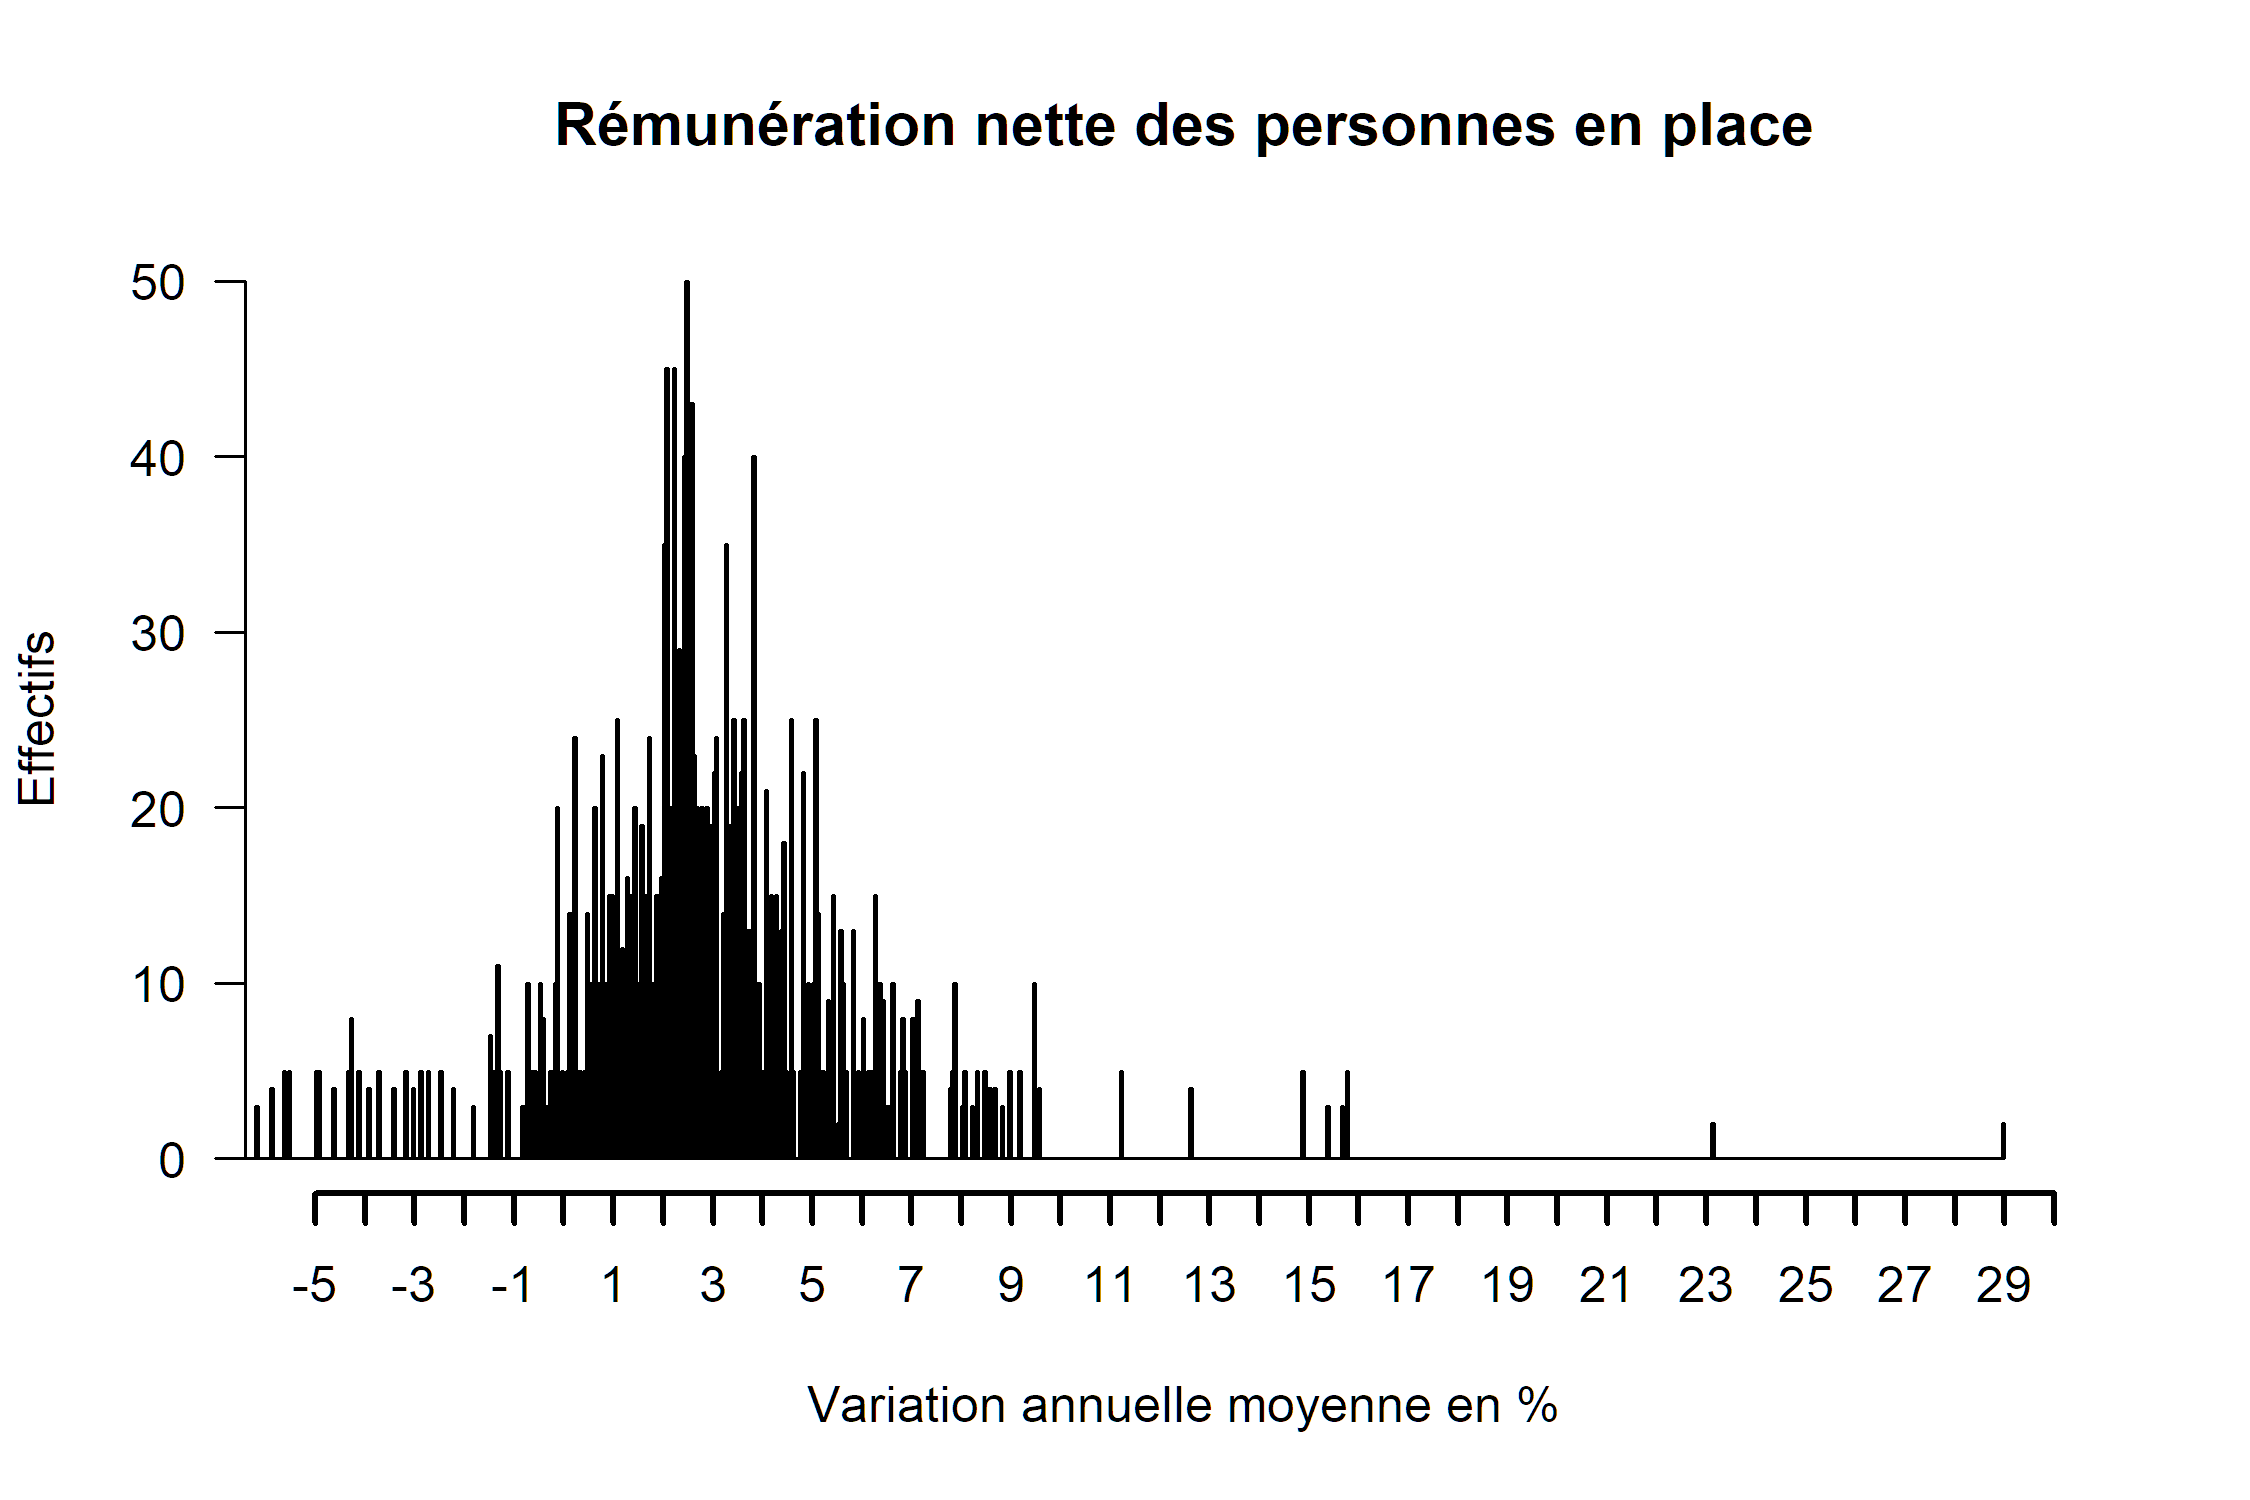
\includegraphics{altair_files/figure-latex/unnamed-chunk-133-1.png}

\emph{Cet histogramme décrit l'évolution de la rémunération moyenne des
personnes en place (RMPP), définies comme présentes deux annees entières
consécutives avec la même quotité}\\
\emph{L'évolution de la RMPP permet d'étudier le glissement
vieillesse-technicité ``positif'', à effectifs constants sur deux
années}

\textbf{Variation individuelle de rémunération nette en EQTP pour les
personnels présents sur toute la periode}

~\emph{Tableau 4.3.1.1}

\begin{longtable}[]{@{}rrrrr@{}}
\toprule
\begin{minipage}[b]{0.12\columnwidth}\raggedleft
Statistique\strut
\end{minipage} & \begin{minipage}[b]{0.22\columnwidth}\raggedleft
Variation normalisée (\%)\strut
\end{minipage} & \begin{minipage}[b]{0.37\columnwidth}\raggedleft
Variation annuelle moyenne normalisée (\%)\strut
\end{minipage} & \begin{minipage}[b]{0.07\columnwidth}\raggedleft
Quotité\strut
\end{minipage} & \begin{minipage}[b]{0.08\columnwidth}\raggedleft
Effectif\strut
\end{minipage}\tabularnewline
\midrule
\endhead
\begin{minipage}[t]{0.12\columnwidth}\raggedleft
Minimum\strut
\end{minipage} & \begin{minipage}[t]{0.22\columnwidth}\raggedleft
-46\strut
\end{minipage} & \begin{minipage}[t]{0.37\columnwidth}\raggedleft
-14\strut
\end{minipage} & \begin{minipage}[t]{0.07\columnwidth}\raggedleft
0,4\strut
\end{minipage} & \begin{minipage}[t]{0.08\columnwidth}\raggedleft
\strut
\end{minipage}\tabularnewline
\begin{minipage}[t]{0.12\columnwidth}\raggedleft
1er quartile\strut
\end{minipage} & \begin{minipage}[t]{0.22\columnwidth}\raggedleft
5,6\strut
\end{minipage} & \begin{minipage}[t]{0.37\columnwidth}\raggedleft
1,4\strut
\end{minipage} & \begin{minipage}[t]{0.07\columnwidth}\raggedleft
1\strut
\end{minipage} & \begin{minipage}[t]{0.08\columnwidth}\raggedleft
\strut
\end{minipage}\tabularnewline
\begin{minipage}[t]{0.12\columnwidth}\raggedleft
Médiane\strut
\end{minipage} & \begin{minipage}[t]{0.22\columnwidth}\raggedleft
10\strut
\end{minipage} & \begin{minipage}[t]{0.37\columnwidth}\raggedleft
2,5\strut
\end{minipage} & \begin{minipage}[t]{0.07\columnwidth}\raggedleft
1\strut
\end{minipage} & \begin{minipage}[t]{0.08\columnwidth}\raggedleft
\strut
\end{minipage}\tabularnewline
\begin{minipage}[t]{0.12\columnwidth}\raggedleft
Moyenne\strut
\end{minipage} & \begin{minipage}[t]{0.22\columnwidth}\raggedleft
12\strut
\end{minipage} & \begin{minipage}[t]{0.37\columnwidth}\raggedleft
2,7\strut
\end{minipage} & \begin{minipage}[t]{0.07\columnwidth}\raggedleft
0,95\strut
\end{minipage} & \begin{minipage}[t]{0.08\columnwidth}\raggedleft
373\strut
\end{minipage}\tabularnewline
\begin{minipage}[t]{0.12\columnwidth}\raggedleft
3ème quartile\strut
\end{minipage} & \begin{minipage}[t]{0.22\columnwidth}\raggedleft
16\strut
\end{minipage} & \begin{minipage}[t]{0.37\columnwidth}\raggedleft
3,8\strut
\end{minipage} & \begin{minipage}[t]{0.07\columnwidth}\raggedleft
1\strut
\end{minipage} & \begin{minipage}[t]{0.08\columnwidth}\raggedleft
\strut
\end{minipage}\tabularnewline
\begin{minipage}[t]{0.12\columnwidth}\raggedleft
Maximum\strut
\end{minipage} & \begin{minipage}[t]{0.22\columnwidth}\raggedleft
123\strut
\end{minipage} & \begin{minipage}[t]{0.37\columnwidth}\raggedleft
22\strut
\end{minipage} & \begin{minipage}[t]{0.07\columnwidth}\raggedleft
1\strut
\end{minipage} & \begin{minipage}[t]{0.08\columnwidth}\raggedleft
\strut
\end{minipage}\tabularnewline
\bottomrule
\end{longtable}

\hypertarget{rmpp-des-titulaires-et-stagiaires}{%
\subsubsection{4.3.2 RMPP des titulaires et
stagiaires}\label{rmpp-des-titulaires-et-stagiaires}}

\textbf{Variation individuelle de rémunération nette en EQTP pour les
personnels présents sur toute la periode}

~\emph{Tableau 4.3.2.1}

\begin{longtable}[]{@{}rrrrr@{}}
\toprule
\begin{minipage}[b]{0.12\columnwidth}\raggedleft
Statistique\strut
\end{minipage} & \begin{minipage}[b]{0.22\columnwidth}\raggedleft
Variation normalisée (\%)\strut
\end{minipage} & \begin{minipage}[b]{0.37\columnwidth}\raggedleft
Variation annuelle moyenne normalisée (\%)\strut
\end{minipage} & \begin{minipage}[b]{0.07\columnwidth}\raggedleft
Quotité\strut
\end{minipage} & \begin{minipage}[b]{0.08\columnwidth}\raggedleft
Effectif\strut
\end{minipage}\tabularnewline
\midrule
\endhead
\begin{minipage}[t]{0.12\columnwidth}\raggedleft
Minimum\strut
\end{minipage} & \begin{minipage}[t]{0.22\columnwidth}\raggedleft
-46\strut
\end{minipage} & \begin{minipage}[t]{0.37\columnwidth}\raggedleft
-14\strut
\end{minipage} & \begin{minipage}[t]{0.07\columnwidth}\raggedleft
0,42\strut
\end{minipage} & \begin{minipage}[t]{0.08\columnwidth}\raggedleft
\strut
\end{minipage}\tabularnewline
\begin{minipage}[t]{0.12\columnwidth}\raggedleft
1er quartile\strut
\end{minipage} & \begin{minipage}[t]{0.22\columnwidth}\raggedleft
5,4\strut
\end{minipage} & \begin{minipage}[t]{0.37\columnwidth}\raggedleft
1,3\strut
\end{minipage} & \begin{minipage}[t]{0.07\columnwidth}\raggedleft
1\strut
\end{minipage} & \begin{minipage}[t]{0.08\columnwidth}\raggedleft
\strut
\end{minipage}\tabularnewline
\begin{minipage}[t]{0.12\columnwidth}\raggedleft
Médiane\strut
\end{minipage} & \begin{minipage}[t]{0.22\columnwidth}\raggedleft
10\strut
\end{minipage} & \begin{minipage}[t]{0.37\columnwidth}\raggedleft
2,5\strut
\end{minipage} & \begin{minipage}[t]{0.07\columnwidth}\raggedleft
1\strut
\end{minipage} & \begin{minipage}[t]{0.08\columnwidth}\raggedleft
\strut
\end{minipage}\tabularnewline
\begin{minipage}[t]{0.12\columnwidth}\raggedleft
Moyenne\strut
\end{minipage} & \begin{minipage}[t]{0.22\columnwidth}\raggedleft
11\strut
\end{minipage} & \begin{minipage}[t]{0.37\columnwidth}\raggedleft
2,6\strut
\end{minipage} & \begin{minipage}[t]{0.07\columnwidth}\raggedleft
0,96\strut
\end{minipage} & \begin{minipage}[t]{0.08\columnwidth}\raggedleft
358\strut
\end{minipage}\tabularnewline
\begin{minipage}[t]{0.12\columnwidth}\raggedleft
3ème quartile\strut
\end{minipage} & \begin{minipage}[t]{0.22\columnwidth}\raggedleft
16\strut
\end{minipage} & \begin{minipage}[t]{0.37\columnwidth}\raggedleft
3,8\strut
\end{minipage} & \begin{minipage}[t]{0.07\columnwidth}\raggedleft
1\strut
\end{minipage} & \begin{minipage}[t]{0.08\columnwidth}\raggedleft
\strut
\end{minipage}\tabularnewline
\begin{minipage}[t]{0.12\columnwidth}\raggedleft
Maximum\strut
\end{minipage} & \begin{minipage}[t]{0.22\columnwidth}\raggedleft
93\strut
\end{minipage} & \begin{minipage}[t]{0.37\columnwidth}\raggedleft
18\strut
\end{minipage} & \begin{minipage}[t]{0.07\columnwidth}\raggedleft
1\strut
\end{minipage} & \begin{minipage}[t]{0.08\columnwidth}\raggedleft
\strut
\end{minipage}\tabularnewline
\bottomrule
\end{longtable}

\href{Bases/Remunerations/Anavar.synthese.csv}{Lien vers la base de
données}

\textbf{Nota}

\emph{Personnes en place :} en fonction au moins deux années
consécutives avec la même quotité sur la periode 2009 à 2013

\emph{Variation sur la periode d'activité :} entre l'arrivée et le
départ de la personne\\
\emph{Variation normalisée :} conforme à la définition INSEE (présente
en début et en fin de période avec la même quotité)

\textbf{Commentaire}

Les différences éventuelles constatées entre l'évolution de la RMPP au
tableau -2 sont dues soit à l'effet de noria soit à l'effet périmètre.

\hypertarget{les-filtres-rmpp-appliques-au-4.3.1-et-4.3.2-ne-sont-plus-appliques.-il-peut-en-resulter-des-variations-significativement-differentes-de-celles-calculees-precedemment.}{%
\subparagraph{Les filtres RMPP appliqués au 4.3.1 et 4.3.2 ne sont plus
appliqués. Il peut en résulter des variations significativement
différentes de celles calculees
précédemment.}\label{les-filtres-rmpp-appliques-au-4.3.1-et-4.3.2-ne-sont-plus-appliques.-il-peut-en-resulter-des-variations-significativement-differentes-de-celles-calculees-precedemment.}}

\hypertarget{effet-de-noria-et-de-variation-deffectifs-sur-remunerations-moyennes}{%
\subsubsection{4.3.3 Effet de noria et de variation d'effectifs sur
rémunérations
moyennes}\label{effet-de-noria-et-de-variation-deffectifs-sur-remunerations-moyennes}}

\emph{Les calculs de RMPP sur la première année de la periode sous revue
sont estimatifs et ne devraient pas être pris en compte pour
publication.}

\textbf{Effet de noria et de variations d'effectifs sur rémunérations
nettes moyennes EQTP}

~\emph{Tableau 4.3.3.1}

\begin{longtable}[]{@{}lllllllll@{}}
\toprule
\begin{minipage}[b]{0.05\columnwidth}\raggedright
Annee\strut
\end{minipage} & \begin{minipage}[b]{0.08\columnwidth}\raggedright
Effectifs\strut
\end{minipage} & \begin{minipage}[b]{0.05\columnwidth}\raggedright
ETPT\strut
\end{minipage} & \begin{minipage}[b]{0.10\columnwidth}\raggedright
ETPT entrants\strut
\end{minipage} & \begin{minipage}[b]{0.10\columnwidth}\raggedright
ETPT sortants\strut
\end{minipage} & \begin{minipage}[b]{0.07\columnwidth}\raggedright
Entrants\strut
\end{minipage} & \begin{minipage}[b]{0.07\columnwidth}\raggedright
Sortants\strut
\end{minipage} & \begin{minipage}[b]{0.11\columnwidth}\raggedright
Var. effectifs\strut
\end{minipage} & \begin{minipage}[b]{0.14\columnwidth}\raggedright
Taux de rotation \%\strut
\end{minipage}\tabularnewline
\midrule
\endhead
\begin{minipage}[t]{0.05\columnwidth}\raggedright
2009\strut
\end{minipage} & \begin{minipage}[t]{0.08\columnwidth}\raggedright
450,0\strut
\end{minipage} & \begin{minipage}[t]{0.05\columnwidth}\raggedright
424,7\strut
\end{minipage} & \begin{minipage}[t]{0.10\columnwidth}\raggedright
9,3\strut
\end{minipage} & \begin{minipage}[t]{0.10\columnwidth}\raggedright
11,4\strut
\end{minipage} & \begin{minipage}[t]{0.07\columnwidth}\raggedright
20,0\strut
\end{minipage} & \begin{minipage}[t]{0.07\columnwidth}\raggedright
21,0\strut
\end{minipage} & \begin{minipage}[t]{0.11\columnwidth}\raggedright
-1,0\strut
\end{minipage} & \begin{minipage}[t]{0.14\columnwidth}\raggedright
4,6\strut
\end{minipage}\tabularnewline
\begin{minipage}[t]{0.05\columnwidth}\raggedright
2010\strut
\end{minipage} & \begin{minipage}[t]{0.08\columnwidth}\raggedright
456,0\strut
\end{minipage} & \begin{minipage}[t]{0.05\columnwidth}\raggedright
431,2\strut
\end{minipage} & \begin{minipage}[t]{0.10\columnwidth}\raggedright
7,1\strut
\end{minipage} & \begin{minipage}[t]{0.10\columnwidth}\raggedright
10,2\strut
\end{minipage} & \begin{minipage}[t]{0.07\columnwidth}\raggedright
16,0\strut
\end{minipage} & \begin{minipage}[t]{0.07\columnwidth}\raggedright
17,0\strut
\end{minipage} & \begin{minipage}[t]{0.11\columnwidth}\raggedright
-1,0\strut
\end{minipage} & \begin{minipage}[t]{0.14\columnwidth}\raggedright
3,6\strut
\end{minipage}\tabularnewline
\begin{minipage}[t]{0.05\columnwidth}\raggedright
2011\strut
\end{minipage} & \begin{minipage}[t]{0.08\columnwidth}\raggedright
451,0\strut
\end{minipage} & \begin{minipage}[t]{0.05\columnwidth}\raggedright
424,9\strut
\end{minipage} & \begin{minipage}[t]{0.10\columnwidth}\raggedright
10,3\strut
\end{minipage} & \begin{minipage}[t]{0.10\columnwidth}\raggedright
12,7\strut
\end{minipage} & \begin{minipage}[t]{0.07\columnwidth}\raggedright
24,0\strut
\end{minipage} & \begin{minipage}[t]{0.07\columnwidth}\raggedright
25,0\strut
\end{minipage} & \begin{minipage}[t]{0.11\columnwidth}\raggedright
-1,0\strut
\end{minipage} & \begin{minipage}[t]{0.14\columnwidth}\raggedright
5,4\strut
\end{minipage}\tabularnewline
\begin{minipage}[t]{0.05\columnwidth}\raggedright
2012\strut
\end{minipage} & \begin{minipage}[t]{0.08\columnwidth}\raggedright
443,0\strut
\end{minipage} & \begin{minipage}[t]{0.05\columnwidth}\raggedright
414,0\strut
\end{minipage} & \begin{minipage}[t]{0.10\columnwidth}\raggedright
13,6\strut
\end{minipage} & \begin{minipage}[t]{0.10\columnwidth}\raggedright
17,2\strut
\end{minipage} & \begin{minipage}[t]{0.07\columnwidth}\raggedright
28,0\strut
\end{minipage} & \begin{minipage}[t]{0.07\columnwidth}\raggedright
35,0\strut
\end{minipage} & \begin{minipage}[t]{0.11\columnwidth}\raggedright
-7,0\strut
\end{minipage} & \begin{minipage}[t]{0.14\columnwidth}\raggedright
7,1\strut
\end{minipage}\tabularnewline
\begin{minipage}[t]{0.05\columnwidth}\raggedright
2013\strut
\end{minipage} & \begin{minipage}[t]{0.08\columnwidth}\raggedright
439,0\strut
\end{minipage} & \begin{minipage}[t]{0.05\columnwidth}\raggedright
417,9\strut
\end{minipage} & \begin{minipage}[t]{0.10\columnwidth}\raggedright
17,1\strut
\end{minipage} & \begin{minipage}[t]{0.10\columnwidth}\raggedright
14,3\strut
\end{minipage} & \begin{minipage}[t]{0.07\columnwidth}\raggedright
35,0\strut
\end{minipage} & \begin{minipage}[t]{0.07\columnwidth}\raggedright
26,0\strut
\end{minipage} & \begin{minipage}[t]{0.11\columnwidth}\raggedright
9,0\strut
\end{minipage} & \begin{minipage}[t]{0.14\columnwidth}\raggedright
6,9\strut
\end{minipage}\tabularnewline
\begin{minipage}[t]{0.05\columnwidth}\raggedright
Total\strut
\end{minipage} & \begin{minipage}[t]{0.08\columnwidth}\raggedright
\strut
\end{minipage} & \begin{minipage}[t]{0.05\columnwidth}\raggedright
\strut
\end{minipage} & \begin{minipage}[t]{0.10\columnwidth}\raggedright
57,5\strut
\end{minipage} & \begin{minipage}[t]{0.10\columnwidth}\raggedright
65,9\strut
\end{minipage} & \begin{minipage}[t]{0.07\columnwidth}\raggedright
123,0\strut
\end{minipage} & \begin{minipage}[t]{0.07\columnwidth}\raggedright
124,0\strut
\end{minipage} & \begin{minipage}[t]{0.11\columnwidth}\raggedright
-1,0\strut
\end{minipage} & \begin{minipage}[t]{0.14\columnwidth}\raggedright
\strut
\end{minipage}\tabularnewline
\bottomrule
\end{longtable}

\begin{longtable}[]{@{}lllllllll@{}}
\toprule
\begin{minipage}[b]{0.05\columnwidth}\raggedright
Annee\strut
\end{minipage} & \begin{minipage}[b]{0.10\columnwidth}\raggedright
Effet noria\strut
\end{minipage} & \begin{minipage}[b]{0.06\columnwidth}\raggedright
\% SMPT\strut
\end{minipage} & \begin{minipage}[b]{0.16\columnwidth}\raggedright
Effet var. effectifs\strut
\end{minipage} & \begin{minipage}[b]{0.06\columnwidth}\raggedright
\% SMPT\strut
\end{minipage} & \begin{minipage}[b]{0.12\columnwidth}\raggedright
Effet vacances\strut
\end{minipage} & \begin{minipage}[b]{0.06\columnwidth}\raggedright
\% SMPT\strut
\end{minipage} & \begin{minipage}[b]{0.09\columnwidth}\raggedright
Total\strut
\end{minipage} & \begin{minipage}[b]{0.06\columnwidth}\raggedright
\% SMPT\strut
\end{minipage}\tabularnewline
\midrule
\endhead
\begin{minipage}[t]{0.05\columnwidth}\raggedright
2009\strut
\end{minipage} & \begin{minipage}[t]{0.10\columnwidth}\raggedright
-54 038,7\strut
\end{minipage} & \begin{minipage}[t]{0.06\columnwidth}\raggedright
-0,7\strut
\end{minipage} & \begin{minipage}[t]{0.16\columnwidth}\raggedright
-5 764,6\strut
\end{minipage} & \begin{minipage}[t]{0.06\columnwidth}\raggedright
-0,1\strut
\end{minipage} & \begin{minipage}[t]{0.12\columnwidth}\raggedright
2 448,2\strut
\end{minipage} & \begin{minipage}[t]{0.06\columnwidth}\raggedright
0,0\strut
\end{minipage} & \begin{minipage}[t]{0.09\columnwidth}\raggedright
-57 355,2\strut
\end{minipage} & \begin{minipage}[t]{0.06\columnwidth}\raggedright
-0,7\strut
\end{minipage}\tabularnewline
\begin{minipage}[t]{0.05\columnwidth}\raggedright
2010\strut
\end{minipage} & \begin{minipage}[t]{0.10\columnwidth}\raggedright
-7 005,5\strut
\end{minipage} & \begin{minipage}[t]{0.06\columnwidth}\raggedright
-0,1\strut
\end{minipage} & \begin{minipage}[t]{0.16\columnwidth}\raggedright
-5 698,9\strut
\end{minipage} & \begin{minipage}[t]{0.06\columnwidth}\raggedright
-0,1\strut
\end{minipage} & \begin{minipage}[t]{0.12\columnwidth}\raggedright
10 338,9\strut
\end{minipage} & \begin{minipage}[t]{0.06\columnwidth}\raggedright
0,1\strut
\end{minipage} & \begin{minipage}[t]{0.09\columnwidth}\raggedright
-2 365,5\strut
\end{minipage} & \begin{minipage}[t]{0.06\columnwidth}\raggedright
-0,0\strut
\end{minipage}\tabularnewline
\begin{minipage}[t]{0.05\columnwidth}\raggedright
2011\strut
\end{minipage} & \begin{minipage}[t]{0.10\columnwidth}\raggedright
-65 883,9\strut
\end{minipage} & \begin{minipage}[t]{0.06\columnwidth}\raggedright
-0,8\strut
\end{minipage} & \begin{minipage}[t]{0.16\columnwidth}\raggedright
-4 940,3\strut
\end{minipage} & \begin{minipage}[t]{0.06\columnwidth}\raggedright
-0,1\strut
\end{minipage} & \begin{minipage}[t]{0.12\columnwidth}\raggedright
-17 673,0\strut
\end{minipage} & \begin{minipage}[t]{0.06\columnwidth}\raggedright
-0,2\strut
\end{minipage} & \begin{minipage}[t]{0.09\columnwidth}\raggedright
-88 497,2\strut
\end{minipage} & \begin{minipage}[t]{0.06\columnwidth}\raggedright
-1,1\strut
\end{minipage}\tabularnewline
\begin{minipage}[t]{0.05\columnwidth}\raggedright
2012\strut
\end{minipage} & \begin{minipage}[t]{0.10\columnwidth}\raggedright
-75 436,2\strut
\end{minipage} & \begin{minipage}[t]{0.06\columnwidth}\raggedright
-1,0\strut
\end{minipage} & \begin{minipage}[t]{0.16\columnwidth}\raggedright
-46 208,4\strut
\end{minipage} & \begin{minipage}[t]{0.06\columnwidth}\raggedright
-0,6\strut
\end{minipage} & \begin{minipage}[t]{0.12\columnwidth}\raggedright
-9 841,5\strut
\end{minipage} & \begin{minipage}[t]{0.06\columnwidth}\raggedright
-0,1\strut
\end{minipage} & \begin{minipage}[t]{0.09\columnwidth}\raggedright
-131 486,1\strut
\end{minipage} & \begin{minipage}[t]{0.06\columnwidth}\raggedright
-1,7\strut
\end{minipage}\tabularnewline
\begin{minipage}[t]{0.05\columnwidth}\raggedright
2013\strut
\end{minipage} & \begin{minipage}[t]{0.10\columnwidth}\raggedright
-17 597,4\strut
\end{minipage} & \begin{minipage}[t]{0.06\columnwidth}\raggedright
-0,2\strut
\end{minipage} & \begin{minipage}[t]{0.16\columnwidth}\raggedright
59 162,6\strut
\end{minipage} & \begin{minipage}[t]{0.06\columnwidth}\raggedright
0,7\strut
\end{minipage} & \begin{minipage}[t]{0.12\columnwidth}\raggedright
13 917,7\strut
\end{minipage} & \begin{minipage}[t]{0.06\columnwidth}\raggedright
0,2\strut
\end{minipage} & \begin{minipage}[t]{0.09\columnwidth}\raggedright
55 483,0\strut
\end{minipage} & \begin{minipage}[t]{0.06\columnwidth}\raggedright
0,7\strut
\end{minipage}\tabularnewline
\begin{minipage}[t]{0.05\columnwidth}\raggedright
Total\strut
\end{minipage} & \begin{minipage}[t]{0.10\columnwidth}\raggedright
-219 961,8\strut
\end{minipage} & \begin{minipage}[t]{0.06\columnwidth}\raggedright
\strut
\end{minipage} & \begin{minipage}[t]{0.16\columnwidth}\raggedright
-3 449,5\strut
\end{minipage} & \begin{minipage}[t]{0.06\columnwidth}\raggedright
\strut
\end{minipage} & \begin{minipage}[t]{0.12\columnwidth}\raggedright
-809,7\strut
\end{minipage} & \begin{minipage}[t]{0.06\columnwidth}\raggedright
\strut
\end{minipage} & \begin{minipage}[t]{0.09\columnwidth}\raggedright
-224 221,0\strut
\end{minipage} & \begin{minipage}[t]{0.06\columnwidth}\raggedright
\strut
\end{minipage}\tabularnewline
\bottomrule
\end{longtable}

\begin{longtable}[]{@{}lllllllll@{}}
\toprule
Annee & RMPP & Entrées n - 1 & Noria & Var. effectifs & Vacances & Total
E/S & Ajustement & SMPT\tabularnewline
\midrule
\endhead
2009 & 18 714,2 & -0,1 & -0,7 & -0,1 & 0,0 & -0,8 & -0,00 & 18
547,7\tabularnewline
2010 & 18 960,9 & -1,2 & -0,1 & -0,1 & 0,1 & -1,2 & -0,01 & 18
563,8\tabularnewline
2011 & 19 048,6 & -0,7 & -0,8 & -0,1 & -0,2 & -1,8 & -0,00 & 18
697,6\tabularnewline
2012 & 19 414,4 & -1,6 & -1,0 & -0,6 & -0,1 & -3,2 & 0,01 & 18
933,2\tabularnewline
2013 & 19 911,6 & -1,1 & -0,2 & 0,7 & 0,2 & -0,4 & -0,03 & 19
324,2\tabularnewline
Moyenne géom. & 19 205,5 & -0,9 & -0,6 & -0,0 & -0,0 & -1,5 & -0,02 & 18
811,1\tabularnewline
\bottomrule
\end{longtable}

\begin{longtable}[]{@{}lllll@{}}
\toprule
Annee & Var. RMPP & Var. effets E/S & Cumul & Var. SMPT\tabularnewline
\midrule
\endhead
2009-2010 & 1,3 & -1,2 & 0,1 & 0,1\tabularnewline
2010-2011 & 0,5 & 0,3 & 0,7 & 0,7\tabularnewline
2011-2012 & 1,9 & -0,6 & 1,3 & 1,3\tabularnewline
2012-2013 & 2,6 & -0,5 & 2,1 & 2,1\tabularnewline
2009-2013 & 6,4 & -2,1 & 4,2 & 4,2\tabularnewline
\bottomrule
\end{longtable}

\textbf{Effet de noria et de variations d'effectifs sur rémunérations
brutes moyennes EQTP}

~\emph{Tableau 4.3.3.2}

\begin{longtable}[]{@{}lllllllll@{}}
\toprule
\begin{minipage}[b]{0.05\columnwidth}\raggedright
Annee\strut
\end{minipage} & \begin{minipage}[b]{0.08\columnwidth}\raggedright
Effectifs\strut
\end{minipage} & \begin{minipage}[b]{0.05\columnwidth}\raggedright
ETPT\strut
\end{minipage} & \begin{minipage}[b]{0.10\columnwidth}\raggedright
ETPT entrants\strut
\end{minipage} & \begin{minipage}[b]{0.10\columnwidth}\raggedright
ETPT sortants\strut
\end{minipage} & \begin{minipage}[b]{0.07\columnwidth}\raggedright
Entrants\strut
\end{minipage} & \begin{minipage}[b]{0.07\columnwidth}\raggedright
Sortants\strut
\end{minipage} & \begin{minipage}[b]{0.11\columnwidth}\raggedright
Var. effectifs\strut
\end{minipage} & \begin{minipage}[b]{0.14\columnwidth}\raggedright
Taux de rotation \%\strut
\end{minipage}\tabularnewline
\midrule
\endhead
\begin{minipage}[t]{0.05\columnwidth}\raggedright
2009\strut
\end{minipage} & \begin{minipage}[t]{0.08\columnwidth}\raggedright
450,0\strut
\end{minipage} & \begin{minipage}[t]{0.05\columnwidth}\raggedright
424,7\strut
\end{minipage} & \begin{minipage}[t]{0.10\columnwidth}\raggedright
9,3\strut
\end{minipage} & \begin{minipage}[t]{0.10\columnwidth}\raggedright
11,4\strut
\end{minipage} & \begin{minipage}[t]{0.07\columnwidth}\raggedright
20,0\strut
\end{minipage} & \begin{minipage}[t]{0.07\columnwidth}\raggedright
21,0\strut
\end{minipage} & \begin{minipage}[t]{0.11\columnwidth}\raggedright
-1,0\strut
\end{minipage} & \begin{minipage}[t]{0.14\columnwidth}\raggedright
4,6\strut
\end{minipage}\tabularnewline
\begin{minipage}[t]{0.05\columnwidth}\raggedright
2010\strut
\end{minipage} & \begin{minipage}[t]{0.08\columnwidth}\raggedright
456,0\strut
\end{minipage} & \begin{minipage}[t]{0.05\columnwidth}\raggedright
431,2\strut
\end{minipage} & \begin{minipage}[t]{0.10\columnwidth}\raggedright
7,1\strut
\end{minipage} & \begin{minipage}[t]{0.10\columnwidth}\raggedright
10,2\strut
\end{minipage} & \begin{minipage}[t]{0.07\columnwidth}\raggedright
16,0\strut
\end{minipage} & \begin{minipage}[t]{0.07\columnwidth}\raggedright
17,0\strut
\end{minipage} & \begin{minipage}[t]{0.11\columnwidth}\raggedright
-1,0\strut
\end{minipage} & \begin{minipage}[t]{0.14\columnwidth}\raggedright
3,6\strut
\end{minipage}\tabularnewline
\begin{minipage}[t]{0.05\columnwidth}\raggedright
2011\strut
\end{minipage} & \begin{minipage}[t]{0.08\columnwidth}\raggedright
451,0\strut
\end{minipage} & \begin{minipage}[t]{0.05\columnwidth}\raggedright
424,9\strut
\end{minipage} & \begin{minipage}[t]{0.10\columnwidth}\raggedright
10,3\strut
\end{minipage} & \begin{minipage}[t]{0.10\columnwidth}\raggedright
12,7\strut
\end{minipage} & \begin{minipage}[t]{0.07\columnwidth}\raggedright
24,0\strut
\end{minipage} & \begin{minipage}[t]{0.07\columnwidth}\raggedright
25,0\strut
\end{minipage} & \begin{minipage}[t]{0.11\columnwidth}\raggedright
-1,0\strut
\end{minipage} & \begin{minipage}[t]{0.14\columnwidth}\raggedright
5,4\strut
\end{minipage}\tabularnewline
\begin{minipage}[t]{0.05\columnwidth}\raggedright
2012\strut
\end{minipage} & \begin{minipage}[t]{0.08\columnwidth}\raggedright
443,0\strut
\end{minipage} & \begin{minipage}[t]{0.05\columnwidth}\raggedright
414,0\strut
\end{minipage} & \begin{minipage}[t]{0.10\columnwidth}\raggedright
13,6\strut
\end{minipage} & \begin{minipage}[t]{0.10\columnwidth}\raggedright
17,2\strut
\end{minipage} & \begin{minipage}[t]{0.07\columnwidth}\raggedright
28,0\strut
\end{minipage} & \begin{minipage}[t]{0.07\columnwidth}\raggedright
35,0\strut
\end{minipage} & \begin{minipage}[t]{0.11\columnwidth}\raggedright
-7,0\strut
\end{minipage} & \begin{minipage}[t]{0.14\columnwidth}\raggedright
7,1\strut
\end{minipage}\tabularnewline
\begin{minipage}[t]{0.05\columnwidth}\raggedright
2013\strut
\end{minipage} & \begin{minipage}[t]{0.08\columnwidth}\raggedright
439,0\strut
\end{minipage} & \begin{minipage}[t]{0.05\columnwidth}\raggedright
417,9\strut
\end{minipage} & \begin{minipage}[t]{0.10\columnwidth}\raggedright
17,1\strut
\end{minipage} & \begin{minipage}[t]{0.10\columnwidth}\raggedright
14,3\strut
\end{minipage} & \begin{minipage}[t]{0.07\columnwidth}\raggedright
35,0\strut
\end{minipage} & \begin{minipage}[t]{0.07\columnwidth}\raggedright
26,0\strut
\end{minipage} & \begin{minipage}[t]{0.11\columnwidth}\raggedright
9,0\strut
\end{minipage} & \begin{minipage}[t]{0.14\columnwidth}\raggedright
6,9\strut
\end{minipage}\tabularnewline
\begin{minipage}[t]{0.05\columnwidth}\raggedright
Total\strut
\end{minipage} & \begin{minipage}[t]{0.08\columnwidth}\raggedright
\strut
\end{minipage} & \begin{minipage}[t]{0.05\columnwidth}\raggedright
\strut
\end{minipage} & \begin{minipage}[t]{0.10\columnwidth}\raggedright
57,5\strut
\end{minipage} & \begin{minipage}[t]{0.10\columnwidth}\raggedright
65,9\strut
\end{minipage} & \begin{minipage}[t]{0.07\columnwidth}\raggedright
123,0\strut
\end{minipage} & \begin{minipage}[t]{0.07\columnwidth}\raggedright
124,0\strut
\end{minipage} & \begin{minipage}[t]{0.11\columnwidth}\raggedright
-1,0\strut
\end{minipage} & \begin{minipage}[t]{0.14\columnwidth}\raggedright
\strut
\end{minipage}\tabularnewline
\bottomrule
\end{longtable}

\begin{longtable}[]{@{}lllllllll@{}}
\toprule
\begin{minipage}[b]{0.05\columnwidth}\raggedright
Annee\strut
\end{minipage} & \begin{minipage}[b]{0.10\columnwidth}\raggedright
Effet noria\strut
\end{minipage} & \begin{minipage}[b]{0.06\columnwidth}\raggedright
\% SMPT\strut
\end{minipage} & \begin{minipage}[b]{0.16\columnwidth}\raggedright
Effet var. effectifs\strut
\end{minipage} & \begin{minipage}[b]{0.06\columnwidth}\raggedright
\% SMPT\strut
\end{minipage} & \begin{minipage}[b]{0.12\columnwidth}\raggedright
Effet vacances\strut
\end{minipage} & \begin{minipage}[b]{0.06\columnwidth}\raggedright
\% SMPT\strut
\end{minipage} & \begin{minipage}[b]{0.09\columnwidth}\raggedright
Total\strut
\end{minipage} & \begin{minipage}[b]{0.06\columnwidth}\raggedright
\% SMPT\strut
\end{minipage}\tabularnewline
\midrule
\endhead
\begin{minipage}[t]{0.05\columnwidth}\raggedright
2009\strut
\end{minipage} & \begin{minipage}[t]{0.10\columnwidth}\raggedright
-68 397,7\strut
\end{minipage} & \begin{minipage}[t]{0.06\columnwidth}\raggedright
-0,7\strut
\end{minipage} & \begin{minipage}[t]{0.16\columnwidth}\raggedright
-6 843,8\strut
\end{minipage} & \begin{minipage}[t]{0.06\columnwidth}\raggedright
-0,1\strut
\end{minipage} & \begin{minipage}[t]{0.12\columnwidth}\raggedright
2 906,5\strut
\end{minipage} & \begin{minipage}[t]{0.06\columnwidth}\raggedright
0,0\strut
\end{minipage} & \begin{minipage}[t]{0.09\columnwidth}\raggedright
-72 335,0\strut
\end{minipage} & \begin{minipage}[t]{0.06\columnwidth}\raggedright
-0,8\strut
\end{minipage}\tabularnewline
\begin{minipage}[t]{0.05\columnwidth}\raggedright
2010\strut
\end{minipage} & \begin{minipage}[t]{0.10\columnwidth}\raggedright
-9 146,0\strut
\end{minipage} & \begin{minipage}[t]{0.06\columnwidth}\raggedright
-0,1\strut
\end{minipage} & \begin{minipage}[t]{0.16\columnwidth}\raggedright
-6 876,1\strut
\end{minipage} & \begin{minipage}[t]{0.06\columnwidth}\raggedright
-0,1\strut
\end{minipage} & \begin{minipage}[t]{0.12\columnwidth}\raggedright
12 474,5\strut
\end{minipage} & \begin{minipage}[t]{0.06\columnwidth}\raggedright
0,1\strut
\end{minipage} & \begin{minipage}[t]{0.09\columnwidth}\raggedright
-3 547,5\strut
\end{minipage} & \begin{minipage}[t]{0.06\columnwidth}\raggedright
-0,0\strut
\end{minipage}\tabularnewline
\begin{minipage}[t]{0.05\columnwidth}\raggedright
2011\strut
\end{minipage} & \begin{minipage}[t]{0.10\columnwidth}\raggedright
-85 990,6\strut
\end{minipage} & \begin{minipage}[t]{0.06\columnwidth}\raggedright
-0,9\strut
\end{minipage} & \begin{minipage}[t]{0.16\columnwidth}\raggedright
-5 908,1\strut
\end{minipage} & \begin{minipage}[t]{0.06\columnwidth}\raggedright
-0,1\strut
\end{minipage} & \begin{minipage}[t]{0.12\columnwidth}\raggedright
-21 135,1\strut
\end{minipage} & \begin{minipage}[t]{0.06\columnwidth}\raggedright
-0,2\strut
\end{minipage} & \begin{minipage}[t]{0.09\columnwidth}\raggedright
-113 033,7\strut
\end{minipage} & \begin{minipage}[t]{0.06\columnwidth}\raggedright
-1,2\strut
\end{minipage}\tabularnewline
\begin{minipage}[t]{0.05\columnwidth}\raggedright
2012\strut
\end{minipage} & \begin{minipage}[t]{0.10\columnwidth}\raggedright
-90 909,0\strut
\end{minipage} & \begin{minipage}[t]{0.06\columnwidth}\raggedright
-0,9\strut
\end{minipage} & \begin{minipage}[t]{0.16\columnwidth}\raggedright
-55 067,5\strut
\end{minipage} & \begin{minipage}[t]{0.06\columnwidth}\raggedright
-0,6\strut
\end{minipage} & \begin{minipage}[t]{0.12\columnwidth}\raggedright
-11 728,3\strut
\end{minipage} & \begin{minipage}[t]{0.06\columnwidth}\raggedright
-0,1\strut
\end{minipage} & \begin{minipage}[t]{0.09\columnwidth}\raggedright
-157 704,8\strut
\end{minipage} & \begin{minipage}[t]{0.06\columnwidth}\raggedright
-1,6\strut
\end{minipage}\tabularnewline
\begin{minipage}[t]{0.05\columnwidth}\raggedright
2013\strut
\end{minipage} & \begin{minipage}[t]{0.10\columnwidth}\raggedright
-19 652,2\strut
\end{minipage} & \begin{minipage}[t]{0.06\columnwidth}\raggedright
-0,2\strut
\end{minipage} & \begin{minipage}[t]{0.16\columnwidth}\raggedright
71 537,1\strut
\end{minipage} & \begin{minipage}[t]{0.06\columnwidth}\raggedright
0,7\strut
\end{minipage} & \begin{minipage}[t]{0.12\columnwidth}\raggedright
16 828,7\strut
\end{minipage} & \begin{minipage}[t]{0.06\columnwidth}\raggedright
0,2\strut
\end{minipage} & \begin{minipage}[t]{0.09\columnwidth}\raggedright
68 713,7\strut
\end{minipage} & \begin{minipage}[t]{0.06\columnwidth}\raggedright
0,7\strut
\end{minipage}\tabularnewline
\begin{minipage}[t]{0.05\columnwidth}\raggedright
Total\strut
\end{minipage} & \begin{minipage}[t]{0.10\columnwidth}\raggedright
-274 095,4\strut
\end{minipage} & \begin{minipage}[t]{0.06\columnwidth}\raggedright
\strut
\end{minipage} & \begin{minipage}[t]{0.16\columnwidth}\raggedright
-3 158,3\strut
\end{minipage} & \begin{minipage}[t]{0.06\columnwidth}\raggedright
\strut
\end{minipage} & \begin{minipage}[t]{0.12\columnwidth}\raggedright
-653,7\strut
\end{minipage} & \begin{minipage}[t]{0.06\columnwidth}\raggedright
\strut
\end{minipage} & \begin{minipage}[t]{0.09\columnwidth}\raggedright
-277 907,4\strut
\end{minipage} & \begin{minipage}[t]{0.06\columnwidth}\raggedright
\strut
\end{minipage}\tabularnewline
\bottomrule
\end{longtable}

\begin{longtable}[]{@{}lllllllll@{}}
\toprule
Annee & RMPP & Entrées n - 1 & Noria & Var. effectifs & Vacances & Total
E/S & Ajustement & SMPT\tabularnewline
\midrule
\endhead
2009 & 22 865,3 & -0,1 & -0,7 & -0,1 & 0,0 & -0,9 & -0,00 & 22
647,9\tabularnewline
2010 & 23 227,1 & -1,3 & -0,1 & -0,1 & 0,1 & -1,3 & -0,01 & 22
709,5\tabularnewline
2011 & 23 444,5 & -0,8 & -0,9 & -0,1 & -0,2 & -2,0 & 0,00 & 22
982,9\tabularnewline
2012 & 23 945,4 & -1,7 & -0,9 & -0,6 & -0,1 & -3,3 & 0,01 & 23
284,1\tabularnewline
2013 & 24 605,9 & -1,3 & -0,2 & 0,7 & 0,2 & -0,6 & -0,03 & 23
809,1\tabularnewline
Moyenne géom. & 23 609,9 & -1,0 & -0,6 & -0,0 & -0,0 & -1,6 & -0,02 & 23
082,8\tabularnewline
\bottomrule
\end{longtable}

\begin{longtable}[]{@{}lllll@{}}
\toprule
Annee & Var. RMPP & Var. effets E/S & Cumul & Var. SMPT\tabularnewline
\midrule
\endhead
2009-2010 & 1,6 & -1,3 & 0,3 & 0,3\tabularnewline
2010-2011 & 0,9 & 0,3 & 1,2 & 1,2\tabularnewline
2011-2012 & 2,1 & -0,8 & 1,3 & 1,3\tabularnewline
2012-2013 & 2,8 & -0,5 & 2,3 & 2,3\tabularnewline
2009-2013 & 7,6 & -2,3 & 5,1 & 5,1\tabularnewline
\bottomrule
\end{longtable}

\emph{Note :}\\
\emph{Effet de noria} : \emph{variation des rémunérations liées au
remplacement de salariés sortants par un même nombre d'entrants.}\\
\emph{Effet des variations d'effectifs (ou de périmètre)} :
\emph{variation des rémunérations liées à la différence entre nombre de
sortants et d'entrants.}\\
\emph{Les effets de vacances d'emploi, s'ils existent, sont intégrés
dans le calcul de l'effet de noria}\\
\emph{Voir les exemples traités en bas de page du lien technique
suivant}\\
\href{Docs/Notices/noria.html}{Spécifications techniques des tables RMPP
et effet de noria}\\
\href{Docs/Notices/GVT\%20et\%20noria.pdf}{Voir complément
méthodologique DGFIP}

\hypertarget{effet-de-noria-et-de-variation-deffectifs-sur-remunerations-moyennes-des-fonctionnaires}{%
\subsubsection{4.3.4 Effet de noria et de variation d'effectifs sur
rémunérations moyennes des
fonctionnaires}\label{effet-de-noria-et-de-variation-deffectifs-sur-remunerations-moyennes-des-fonctionnaires}}

\textbf{Effet de noria et de variations d'effectifs sur rémunérations
nettes moyennes EQTP des fonctionnaires}

~\emph{Tableau 4.3.4.1}

\begin{longtable}[]{@{}lllllllll@{}}
\toprule
\begin{minipage}[b]{0.05\columnwidth}\raggedright
Annee\strut
\end{minipage} & \begin{minipage}[b]{0.08\columnwidth}\raggedright
Effectifs\strut
\end{minipage} & \begin{minipage}[b]{0.05\columnwidth}\raggedright
ETPT\strut
\end{minipage} & \begin{minipage}[b]{0.10\columnwidth}\raggedright
ETPT entrants\strut
\end{minipage} & \begin{minipage}[b]{0.10\columnwidth}\raggedright
ETPT sortants\strut
\end{minipage} & \begin{minipage}[b]{0.07\columnwidth}\raggedright
Entrants\strut
\end{minipage} & \begin{minipage}[b]{0.07\columnwidth}\raggedright
Sortants\strut
\end{minipage} & \begin{minipage}[b]{0.11\columnwidth}\raggedright
Var. effectifs\strut
\end{minipage} & \begin{minipage}[b]{0.14\columnwidth}\raggedright
Taux de rotation \%\strut
\end{minipage}\tabularnewline
\midrule
\endhead
\begin{minipage}[t]{0.05\columnwidth}\raggedright
2009\strut
\end{minipage} & \begin{minipage}[t]{0.08\columnwidth}\raggedright
400,0\strut
\end{minipage} & \begin{minipage}[t]{0.05\columnwidth}\raggedright
381,7\strut
\end{minipage} & \begin{minipage}[t]{0.10\columnwidth}\raggedright
4,0\strut
\end{minipage} & \begin{minipage}[t]{0.10\columnwidth}\raggedright
6,2\strut
\end{minipage} & \begin{minipage}[t]{0.07\columnwidth}\raggedright
7,0\strut
\end{minipage} & \begin{minipage}[t]{0.07\columnwidth}\raggedright
10,0\strut
\end{minipage} & \begin{minipage}[t]{0.11\columnwidth}\raggedright
-3,0\strut
\end{minipage} & \begin{minipage}[t]{0.14\columnwidth}\raggedright
2,1\strut
\end{minipage}\tabularnewline
\begin{minipage}[t]{0.05\columnwidth}\raggedright
2010\strut
\end{minipage} & \begin{minipage}[t]{0.08\columnwidth}\raggedright
403,0\strut
\end{minipage} & \begin{minipage}[t]{0.05\columnwidth}\raggedright
386,3\strut
\end{minipage} & \begin{minipage}[t]{0.10\columnwidth}\raggedright
2,6\strut
\end{minipage} & \begin{minipage}[t]{0.10\columnwidth}\raggedright
4,5\strut
\end{minipage} & \begin{minipage}[t]{0.07\columnwidth}\raggedright
5,0\strut
\end{minipage} & \begin{minipage}[t]{0.07\columnwidth}\raggedright
6,0\strut
\end{minipage} & \begin{minipage}[t]{0.11\columnwidth}\raggedright
-1,0\strut
\end{minipage} & \begin{minipage}[t]{0.14\columnwidth}\raggedright
1,4\strut
\end{minipage}\tabularnewline
\begin{minipage}[t]{0.05\columnwidth}\raggedright
2011\strut
\end{minipage} & \begin{minipage}[t]{0.08\columnwidth}\raggedright
401,0\strut
\end{minipage} & \begin{minipage}[t]{0.05\columnwidth}\raggedright
378,8\strut
\end{minipage} & \begin{minipage}[t]{0.10\columnwidth}\raggedright
2,1\strut
\end{minipage} & \begin{minipage}[t]{0.10\columnwidth}\raggedright
5,4\strut
\end{minipage} & \begin{minipage}[t]{0.07\columnwidth}\raggedright
4,0\strut
\end{minipage} & \begin{minipage}[t]{0.07\columnwidth}\raggedright
10,0\strut
\end{minipage} & \begin{minipage}[t]{0.11\columnwidth}\raggedright
-6,0\strut
\end{minipage} & \begin{minipage}[t]{0.14\columnwidth}\raggedright
1,7\strut
\end{minipage}\tabularnewline
\begin{minipage}[t]{0.05\columnwidth}\raggedright
2012\strut
\end{minipage} & \begin{minipage}[t]{0.08\columnwidth}\raggedright
393,0\strut
\end{minipage} & \begin{minipage}[t]{0.05\columnwidth}\raggedright
370,1\strut
\end{minipage} & \begin{minipage}[t]{0.10\columnwidth}\raggedright
6,0\strut
\end{minipage} & \begin{minipage}[t]{0.10\columnwidth}\raggedright
9,0\strut
\end{minipage} & \begin{minipage}[t]{0.07\columnwidth}\raggedright
11,0\strut
\end{minipage} & \begin{minipage}[t]{0.07\columnwidth}\raggedright
19,0\strut
\end{minipage} & \begin{minipage}[t]{0.11\columnwidth}\raggedright
-8,0\strut
\end{minipage} & \begin{minipage}[t]{0.14\columnwidth}\raggedright
3,8\strut
\end{minipage}\tabularnewline
\begin{minipage}[t]{0.05\columnwidth}\raggedright
2013\strut
\end{minipage} & \begin{minipage}[t]{0.08\columnwidth}\raggedright
386,0\strut
\end{minipage} & \begin{minipage}[t]{0.05\columnwidth}\raggedright
367,7\strut
\end{minipage} & \begin{minipage}[t]{0.10\columnwidth}\raggedright
3,4\strut
\end{minipage} & \begin{minipage}[t]{0.10\columnwidth}\raggedright
3,8\strut
\end{minipage} & \begin{minipage}[t]{0.07\columnwidth}\raggedright
6,0\strut
\end{minipage} & \begin{minipage}[t]{0.07\columnwidth}\raggedright
7,0\strut
\end{minipage} & \begin{minipage}[t]{0.11\columnwidth}\raggedright
-1,0\strut
\end{minipage} & \begin{minipage}[t]{0.14\columnwidth}\raggedright
1,7\strut
\end{minipage}\tabularnewline
\begin{minipage}[t]{0.05\columnwidth}\raggedright
Total\strut
\end{minipage} & \begin{minipage}[t]{0.08\columnwidth}\raggedright
\strut
\end{minipage} & \begin{minipage}[t]{0.05\columnwidth}\raggedright
\strut
\end{minipage} & \begin{minipage}[t]{0.10\columnwidth}\raggedright
18,1\strut
\end{minipage} & \begin{minipage}[t]{0.10\columnwidth}\raggedright
29,0\strut
\end{minipage} & \begin{minipage}[t]{0.07\columnwidth}\raggedright
33,0\strut
\end{minipage} & \begin{minipage}[t]{0.07\columnwidth}\raggedright
52,0\strut
\end{minipage} & \begin{minipage}[t]{0.11\columnwidth}\raggedright
-19,0\strut
\end{minipage} & \begin{minipage}[t]{0.14\columnwidth}\raggedright
\strut
\end{minipage}\tabularnewline
\bottomrule
\end{longtable}

\begin{longtable}[]{@{}lllllllll@{}}
\toprule
\begin{minipage}[b]{0.05\columnwidth}\raggedright
Annee\strut
\end{minipage} & \begin{minipage}[b]{0.10\columnwidth}\raggedright
Effet noria\strut
\end{minipage} & \begin{minipage}[b]{0.06\columnwidth}\raggedright
\% SMPT\strut
\end{minipage} & \begin{minipage}[b]{0.16\columnwidth}\raggedright
Effet var. effectifs\strut
\end{minipage} & \begin{minipage}[b]{0.06\columnwidth}\raggedright
\% SMPT\strut
\end{minipage} & \begin{minipage}[b]{0.12\columnwidth}\raggedright
Effet vacances\strut
\end{minipage} & \begin{minipage}[b]{0.06\columnwidth}\raggedright
\% SMPT\strut
\end{minipage} & \begin{minipage}[b]{0.09\columnwidth}\raggedright
Total\strut
\end{minipage} & \begin{minipage}[b]{0.06\columnwidth}\raggedright
\% SMPT\strut
\end{minipage}\tabularnewline
\midrule
\endhead
\begin{minipage}[t]{0.05\columnwidth}\raggedright
2009\strut
\end{minipage} & \begin{minipage}[t]{0.10\columnwidth}\raggedright
-36 002,3\strut
\end{minipage} & \begin{minipage}[t]{0.06\columnwidth}\raggedright
-0,5\strut
\end{minipage} & \begin{minipage}[t]{0.16\columnwidth}\raggedright
-21 643,2\strut
\end{minipage} & \begin{minipage}[t]{0.06\columnwidth}\raggedright
-0,3\strut
\end{minipage} & \begin{minipage}[t]{0.12\columnwidth}\raggedright
24 300,0\strut
\end{minipage} & \begin{minipage}[t]{0.06\columnwidth}\raggedright
0,3\strut
\end{minipage} & \begin{minipage}[t]{0.09\columnwidth}\raggedright
-33 345,5\strut
\end{minipage} & \begin{minipage}[t]{0.06\columnwidth}\raggedright
-0,5\strut
\end{minipage}\tabularnewline
\begin{minipage}[t]{0.05\columnwidth}\raggedright
2010\strut
\end{minipage} & \begin{minipage}[t]{0.10\columnwidth}\raggedright
-3 329,3\strut
\end{minipage} & \begin{minipage}[t]{0.06\columnwidth}\raggedright
-0,0\strut
\end{minipage} & \begin{minipage}[t]{0.16\columnwidth}\raggedright
-7 995,5\strut
\end{minipage} & \begin{minipage}[t]{0.06\columnwidth}\raggedright
-0,1\strut
\end{minipage} & \begin{minipage}[t]{0.12\columnwidth}\raggedright
24 652,9\strut
\end{minipage} & \begin{minipage}[t]{0.06\columnwidth}\raggedright
0,3\strut
\end{minipage} & \begin{minipage}[t]{0.09\columnwidth}\raggedright
13 328,1\strut
\end{minipage} & \begin{minipage}[t]{0.06\columnwidth}\raggedright
0,2\strut
\end{minipage}\tabularnewline
\begin{minipage}[t]{0.05\columnwidth}\raggedright
2011\strut
\end{minipage} & \begin{minipage}[t]{0.10\columnwidth}\raggedright
-20 411,5\strut
\end{minipage} & \begin{minipage}[t]{0.06\columnwidth}\raggedright
-0,3\strut
\end{minipage} & \begin{minipage}[t]{0.16\columnwidth}\raggedright
-51 098,6\strut
\end{minipage} & \begin{minipage}[t]{0.06\columnwidth}\raggedright
-0,7\strut
\end{minipage} & \begin{minipage}[t]{0.12\columnwidth}\raggedright
12 814,3\strut
\end{minipage} & \begin{minipage}[t]{0.06\columnwidth}\raggedright
0,2\strut
\end{minipage} & \begin{minipage}[t]{0.09\columnwidth}\raggedright
-58 695,7\strut
\end{minipage} & \begin{minipage}[t]{0.06\columnwidth}\raggedright
-0,8\strut
\end{minipage}\tabularnewline
\begin{minipage}[t]{0.05\columnwidth}\raggedright
2012\strut
\end{minipage} & \begin{minipage}[t]{0.10\columnwidth}\raggedright
-70 403,4\strut
\end{minipage} & \begin{minipage}[t]{0.06\columnwidth}\raggedright
-1,0\strut
\end{minipage} & \begin{minipage}[t]{0.16\columnwidth}\raggedright
-72 436,2\strut
\end{minipage} & \begin{minipage}[t]{0.06\columnwidth}\raggedright
-1,0\strut
\end{minipage} & \begin{minipage}[t]{0.12\columnwidth}\raggedright
7 302,7\strut
\end{minipage} & \begin{minipage}[t]{0.06\columnwidth}\raggedright
0,1\strut
\end{minipage} & \begin{minipage}[t]{0.09\columnwidth}\raggedright
-135 536,9\strut
\end{minipage} & \begin{minipage}[t]{0.06\columnwidth}\raggedright
-1,9\strut
\end{minipage}\tabularnewline
\begin{minipage}[t]{0.05\columnwidth}\raggedright
2013\strut
\end{minipage} & \begin{minipage}[t]{0.10\columnwidth}\raggedright
-14 655,8\strut
\end{minipage} & \begin{minipage}[t]{0.06\columnwidth}\raggedright
-0,2\strut
\end{minipage} & \begin{minipage}[t]{0.16\columnwidth}\raggedright
-9 052,2\strut
\end{minipage} & \begin{minipage}[t]{0.06\columnwidth}\raggedright
-0,1\strut
\end{minipage} & \begin{minipage}[t]{0.12\columnwidth}\raggedright
11 317,0\strut
\end{minipage} & \begin{minipage}[t]{0.06\columnwidth}\raggedright
0,2\strut
\end{minipage} & \begin{minipage}[t]{0.09\columnwidth}\raggedright
-12 391,1\strut
\end{minipage} & \begin{minipage}[t]{0.06\columnwidth}\raggedright
-0,2\strut
\end{minipage}\tabularnewline
\begin{minipage}[t]{0.05\columnwidth}\raggedright
Total\strut
\end{minipage} & \begin{minipage}[t]{0.10\columnwidth}\raggedright
-144 802,3\strut
\end{minipage} & \begin{minipage}[t]{0.06\columnwidth}\raggedright
\strut
\end{minipage} & \begin{minipage}[t]{0.16\columnwidth}\raggedright
-162 225,8\strut
\end{minipage} & \begin{minipage}[t]{0.06\columnwidth}\raggedright
\strut
\end{minipage} & \begin{minipage}[t]{0.12\columnwidth}\raggedright
80 386,9\strut
\end{minipage} & \begin{minipage}[t]{0.06\columnwidth}\raggedright
\strut
\end{minipage} & \begin{minipage}[t]{0.09\columnwidth}\raggedright
-226 641,2\strut
\end{minipage} & \begin{minipage}[t]{0.06\columnwidth}\raggedright
\strut
\end{minipage}\tabularnewline
\bottomrule
\end{longtable}

\begin{longtable}[]{@{}lllllllll@{}}
\toprule
Annee & RMPP & Entrées n - 1 & Noria & Var. effectifs & Vacances & Total
E/S & Ajustement & SMPT\tabularnewline
\midrule
\endhead
2009 & 18 885,8 & 0,1 & -0,5 & -0,3 & 0,3 & -0,3 & 0,00 & 18
902,5\tabularnewline
2010 & 19 091,6 & -0,5 & -0,0 & -0,1 & 0,3 & -0,3 & -0,00 & 18
952,1\tabularnewline
2011 & 19 207,2 & -0,3 & -0,3 & -0,7 & 0,2 & -1,1 & 0,01 & 19
157,5\tabularnewline
2012 & 19 526,2 & -0,4 & -1,0 & -1,0 & 0,1 & -2,2 & 0,02 & 19
508,7\tabularnewline
2013 & 20 009,7 & -0,2 & -0,2 & -0,1 & 0,2 & -0,4 & 0,00 & 19
943,1\tabularnewline
Moyenne géom. & 19 340,1 & -0,2 & -0,4 & -0,5 & 0,2 & -0,9 & -0,00 & 19
288,9\tabularnewline
\bottomrule
\end{longtable}

\begin{longtable}[]{@{}lllll@{}}
\toprule
Annee & Var. RMPP & Var. effets E/S & Cumul & Var. SMPT\tabularnewline
\midrule
\endhead
2009-2010 & 1,1 & -0,8 & 0,3 & 0,3\tabularnewline
2010-2011 & 0,6 & 0,5 & 1,1 & 1,1\tabularnewline
2011-2012 & 1,7 & 0,2 & 1,8 & 1,8\tabularnewline
2012-2013 & 2,5 & -0,2 & 2,2 & 2,2\tabularnewline
2009-2013 & 6,0 & -0,4 & 5,5 & 5,5\tabularnewline
\bottomrule
\end{longtable}

\textbf{Effet de noria et de variations d'effectifs sur rémunérations
brutes moyennes EQTP des fonctionnaires}

~\emph{Tableau 4.3.4.2}

\begin{longtable}[]{@{}lllllllll@{}}
\toprule
\begin{minipage}[b]{0.05\columnwidth}\raggedright
Annee\strut
\end{minipage} & \begin{minipage}[b]{0.08\columnwidth}\raggedright
Effectifs\strut
\end{minipage} & \begin{minipage}[b]{0.05\columnwidth}\raggedright
ETPT\strut
\end{minipage} & \begin{minipage}[b]{0.10\columnwidth}\raggedright
ETPT entrants\strut
\end{minipage} & \begin{minipage}[b]{0.10\columnwidth}\raggedright
ETPT sortants\strut
\end{minipage} & \begin{minipage}[b]{0.07\columnwidth}\raggedright
Entrants\strut
\end{minipage} & \begin{minipage}[b]{0.07\columnwidth}\raggedright
Sortants\strut
\end{minipage} & \begin{minipage}[b]{0.11\columnwidth}\raggedright
Var. effectifs\strut
\end{minipage} & \begin{minipage}[b]{0.14\columnwidth}\raggedright
Taux de rotation \%\strut
\end{minipage}\tabularnewline
\midrule
\endhead
\begin{minipage}[t]{0.05\columnwidth}\raggedright
2009\strut
\end{minipage} & \begin{minipage}[t]{0.08\columnwidth}\raggedright
400,0\strut
\end{minipage} & \begin{minipage}[t]{0.05\columnwidth}\raggedright
381,7\strut
\end{minipage} & \begin{minipage}[t]{0.10\columnwidth}\raggedright
4,0\strut
\end{minipage} & \begin{minipage}[t]{0.10\columnwidth}\raggedright
6,2\strut
\end{minipage} & \begin{minipage}[t]{0.07\columnwidth}\raggedright
7,0\strut
\end{minipage} & \begin{minipage}[t]{0.07\columnwidth}\raggedright
10,0\strut
\end{minipage} & \begin{minipage}[t]{0.11\columnwidth}\raggedright
-3,0\strut
\end{minipage} & \begin{minipage}[t]{0.14\columnwidth}\raggedright
2,1\strut
\end{minipage}\tabularnewline
\begin{minipage}[t]{0.05\columnwidth}\raggedright
2010\strut
\end{minipage} & \begin{minipage}[t]{0.08\columnwidth}\raggedright
403,0\strut
\end{minipage} & \begin{minipage}[t]{0.05\columnwidth}\raggedright
386,3\strut
\end{minipage} & \begin{minipage}[t]{0.10\columnwidth}\raggedright
2,6\strut
\end{minipage} & \begin{minipage}[t]{0.10\columnwidth}\raggedright
4,5\strut
\end{minipage} & \begin{minipage}[t]{0.07\columnwidth}\raggedright
5,0\strut
\end{minipage} & \begin{minipage}[t]{0.07\columnwidth}\raggedright
6,0\strut
\end{minipage} & \begin{minipage}[t]{0.11\columnwidth}\raggedright
-1,0\strut
\end{minipage} & \begin{minipage}[t]{0.14\columnwidth}\raggedright
1,4\strut
\end{minipage}\tabularnewline
\begin{minipage}[t]{0.05\columnwidth}\raggedright
2011\strut
\end{minipage} & \begin{minipage}[t]{0.08\columnwidth}\raggedright
401,0\strut
\end{minipage} & \begin{minipage}[t]{0.05\columnwidth}\raggedright
378,8\strut
\end{minipage} & \begin{minipage}[t]{0.10\columnwidth}\raggedright
2,1\strut
\end{minipage} & \begin{minipage}[t]{0.10\columnwidth}\raggedright
5,4\strut
\end{minipage} & \begin{minipage}[t]{0.07\columnwidth}\raggedright
4,0\strut
\end{minipage} & \begin{minipage}[t]{0.07\columnwidth}\raggedright
10,0\strut
\end{minipage} & \begin{minipage}[t]{0.11\columnwidth}\raggedright
-6,0\strut
\end{minipage} & \begin{minipage}[t]{0.14\columnwidth}\raggedright
1,7\strut
\end{minipage}\tabularnewline
\begin{minipage}[t]{0.05\columnwidth}\raggedright
2012\strut
\end{minipage} & \begin{minipage}[t]{0.08\columnwidth}\raggedright
393,0\strut
\end{minipage} & \begin{minipage}[t]{0.05\columnwidth}\raggedright
370,1\strut
\end{minipage} & \begin{minipage}[t]{0.10\columnwidth}\raggedright
6,0\strut
\end{minipage} & \begin{minipage}[t]{0.10\columnwidth}\raggedright
9,0\strut
\end{minipage} & \begin{minipage}[t]{0.07\columnwidth}\raggedright
11,0\strut
\end{minipage} & \begin{minipage}[t]{0.07\columnwidth}\raggedright
19,0\strut
\end{minipage} & \begin{minipage}[t]{0.11\columnwidth}\raggedright
-8,0\strut
\end{minipage} & \begin{minipage}[t]{0.14\columnwidth}\raggedright
3,8\strut
\end{minipage}\tabularnewline
\begin{minipage}[t]{0.05\columnwidth}\raggedright
2013\strut
\end{minipage} & \begin{minipage}[t]{0.08\columnwidth}\raggedright
386,0\strut
\end{minipage} & \begin{minipage}[t]{0.05\columnwidth}\raggedright
367,7\strut
\end{minipage} & \begin{minipage}[t]{0.10\columnwidth}\raggedright
3,4\strut
\end{minipage} & \begin{minipage}[t]{0.10\columnwidth}\raggedright
3,8\strut
\end{minipage} & \begin{minipage}[t]{0.07\columnwidth}\raggedright
6,0\strut
\end{minipage} & \begin{minipage}[t]{0.07\columnwidth}\raggedright
7,0\strut
\end{minipage} & \begin{minipage}[t]{0.11\columnwidth}\raggedright
-1,0\strut
\end{minipage} & \begin{minipage}[t]{0.14\columnwidth}\raggedright
1,7\strut
\end{minipage}\tabularnewline
\begin{minipage}[t]{0.05\columnwidth}\raggedright
Total\strut
\end{minipage} & \begin{minipage}[t]{0.08\columnwidth}\raggedright
\strut
\end{minipage} & \begin{minipage}[t]{0.05\columnwidth}\raggedright
\strut
\end{minipage} & \begin{minipage}[t]{0.10\columnwidth}\raggedright
18,1\strut
\end{minipage} & \begin{minipage}[t]{0.10\columnwidth}\raggedright
29,0\strut
\end{minipage} & \begin{minipage}[t]{0.07\columnwidth}\raggedright
33,0\strut
\end{minipage} & \begin{minipage}[t]{0.07\columnwidth}\raggedright
52,0\strut
\end{minipage} & \begin{minipage}[t]{0.11\columnwidth}\raggedright
-19,0\strut
\end{minipage} & \begin{minipage}[t]{0.14\columnwidth}\raggedright
\strut
\end{minipage}\tabularnewline
\bottomrule
\end{longtable}

\begin{longtable}[]{@{}lllllllll@{}}
\toprule
\begin{minipage}[b]{0.05\columnwidth}\raggedright
Annee\strut
\end{minipage} & \begin{minipage}[b]{0.10\columnwidth}\raggedright
Effet noria\strut
\end{minipage} & \begin{minipage}[b]{0.06\columnwidth}\raggedright
\% SMPT\strut
\end{minipage} & \begin{minipage}[b]{0.16\columnwidth}\raggedright
Effet var. effectifs\strut
\end{minipage} & \begin{minipage}[b]{0.06\columnwidth}\raggedright
\% SMPT\strut
\end{minipage} & \begin{minipage}[b]{0.12\columnwidth}\raggedright
Effet vacances\strut
\end{minipage} & \begin{minipage}[b]{0.06\columnwidth}\raggedright
\% SMPT\strut
\end{minipage} & \begin{minipage}[b]{0.09\columnwidth}\raggedright
Total\strut
\end{minipage} & \begin{minipage}[b]{0.06\columnwidth}\raggedright
\% SMPT\strut
\end{minipage}\tabularnewline
\midrule
\endhead
\begin{minipage}[t]{0.05\columnwidth}\raggedright
2009\strut
\end{minipage} & \begin{minipage}[t]{0.10\columnwidth}\raggedright
-44 644,4\strut
\end{minipage} & \begin{minipage}[t]{0.06\columnwidth}\raggedright
-0,5\strut
\end{minipage} & \begin{minipage}[t]{0.16\columnwidth}\raggedright
-25 859,9\strut
\end{minipage} & \begin{minipage}[t]{0.06\columnwidth}\raggedright
-0,3\strut
\end{minipage} & \begin{minipage}[t]{0.12\columnwidth}\raggedright
29 034,3\strut
\end{minipage} & \begin{minipage}[t]{0.06\columnwidth}\raggedright
0,3\strut
\end{minipage} & \begin{minipage}[t]{0.09\columnwidth}\raggedright
-41 470,0\strut
\end{minipage} & \begin{minipage}[t]{0.06\columnwidth}\raggedright
-0,5\strut
\end{minipage}\tabularnewline
\begin{minipage}[t]{0.05\columnwidth}\raggedright
2010\strut
\end{minipage} & \begin{minipage}[t]{0.10\columnwidth}\raggedright
-5 014,7\strut
\end{minipage} & \begin{minipage}[t]{0.06\columnwidth}\raggedright
-0,1\strut
\end{minipage} & \begin{minipage}[t]{0.16\columnwidth}\raggedright
-9 611,2\strut
\end{minipage} & \begin{minipage}[t]{0.06\columnwidth}\raggedright
-0,1\strut
\end{minipage} & \begin{minipage}[t]{0.12\columnwidth}\raggedright
29 634,5\strut
\end{minipage} & \begin{minipage}[t]{0.06\columnwidth}\raggedright
0,3\strut
\end{minipage} & \begin{minipage}[t]{0.09\columnwidth}\raggedright
15 008,5\strut
\end{minipage} & \begin{minipage}[t]{0.06\columnwidth}\raggedright
0,2\strut
\end{minipage}\tabularnewline
\begin{minipage}[t]{0.05\columnwidth}\raggedright
2011\strut
\end{minipage} & \begin{minipage}[t]{0.10\columnwidth}\raggedright
-27 545,5\strut
\end{minipage} & \begin{minipage}[t]{0.06\columnwidth}\raggedright
-0,3\strut
\end{minipage} & \begin{minipage}[t]{0.16\columnwidth}\raggedright
-61 244,8\strut
\end{minipage} & \begin{minipage}[t]{0.06\columnwidth}\raggedright
-0,7\strut
\end{minipage} & \begin{minipage}[t]{0.12\columnwidth}\raggedright
15 358,7\strut
\end{minipage} & \begin{minipage}[t]{0.06\columnwidth}\raggedright
0,2\strut
\end{minipage} & \begin{minipage}[t]{0.09\columnwidth}\raggedright
-73 431,6\strut
\end{minipage} & \begin{minipage}[t]{0.06\columnwidth}\raggedright
-0,8\strut
\end{minipage}\tabularnewline
\begin{minipage}[t]{0.05\columnwidth}\raggedright
2012\strut
\end{minipage} & \begin{minipage}[t]{0.10\columnwidth}\raggedright
-89 444,9\strut
\end{minipage} & \begin{minipage}[t]{0.06\columnwidth}\raggedright
-1,0\strut
\end{minipage} & \begin{minipage}[t]{0.16\columnwidth}\raggedright
-86 114,5\strut
\end{minipage} & \begin{minipage}[t]{0.06\columnwidth}\raggedright
-1,0\strut
\end{minipage} & \begin{minipage}[t]{0.12\columnwidth}\raggedright
8 681,7\strut
\end{minipage} & \begin{minipage}[t]{0.06\columnwidth}\raggedright
0,1\strut
\end{minipage} & \begin{minipage}[t]{0.09\columnwidth}\raggedright
-166 877,7\strut
\end{minipage} & \begin{minipage}[t]{0.06\columnwidth}\raggedright
-1,9\strut
\end{minipage}\tabularnewline
\begin{minipage}[t]{0.05\columnwidth}\raggedright
2013\strut
\end{minipage} & \begin{minipage}[t]{0.10\columnwidth}\raggedright
-17 336,4\strut
\end{minipage} & \begin{minipage}[t]{0.06\columnwidth}\raggedright
-0,2\strut
\end{minipage} & \begin{minipage}[t]{0.16\columnwidth}\raggedright
-11 098,3\strut
\end{minipage} & \begin{minipage}[t]{0.06\columnwidth}\raggedright
-0,1\strut
\end{minipage} & \begin{minipage}[t]{0.12\columnwidth}\raggedright
13 874,9\strut
\end{minipage} & \begin{minipage}[t]{0.06\columnwidth}\raggedright
0,2\strut
\end{minipage} & \begin{minipage}[t]{0.09\columnwidth}\raggedright
-14 559,7\strut
\end{minipage} & \begin{minipage}[t]{0.06\columnwidth}\raggedright
-0,2\strut
\end{minipage}\tabularnewline
\begin{minipage}[t]{0.05\columnwidth}\raggedright
Total\strut
\end{minipage} & \begin{minipage}[t]{0.10\columnwidth}\raggedright
-183 985,9\strut
\end{minipage} & \begin{minipage}[t]{0.06\columnwidth}\raggedright
\strut
\end{minipage} & \begin{minipage}[t]{0.16\columnwidth}\raggedright
-193 928,7\strut
\end{minipage} & \begin{minipage}[t]{0.06\columnwidth}\raggedright
\strut
\end{minipage} & \begin{minipage}[t]{0.12\columnwidth}\raggedright
96 584,1\strut
\end{minipage} & \begin{minipage}[t]{0.06\columnwidth}\raggedright
\strut
\end{minipage} & \begin{minipage}[t]{0.09\columnwidth}\raggedright
-281 330,4\strut
\end{minipage} & \begin{minipage}[t]{0.06\columnwidth}\raggedright
\strut
\end{minipage}\tabularnewline
\bottomrule
\end{longtable}

\begin{longtable}[]{@{}lllllllll@{}}
\toprule
Annee & RMPP & Entrées n - 1 & Noria & Var. effectifs & Vacances & Total
E/S & Ajustement & SMPT\tabularnewline
\midrule
\endhead
2009 & 23 083,7 & 0,2 & -0,5 & -0,3 & 0,3 & -0,3 & 0,00 & 23
099,7\tabularnewline
2010 & 23 404,5 & -0,6 & -0,1 & -0,1 & 0,3 & -0,5 & -0,00 & 23
211,7\tabularnewline
2011 & 23 664,6 & -0,3 & -0,3 & -0,7 & 0,2 & -1,1 & 0,01 & 23
586,8\tabularnewline
2012 & 24 101,5 & -0,4 & -1,0 & -1,0 & 0,1 & -2,3 & 0,02 & 24
036,6\tabularnewline
2013 & 24 740,0 & -0,4 & -0,2 & -0,1 & 0,2 & -0,5 & 0,00 & 24
613,1\tabularnewline
Moyenne géom. & 23 791,9 & -0,3 & -0,4 & -0,4 & 0,2 & -1,0 & -0,00 & 23
703,1\tabularnewline
\bottomrule
\end{longtable}

\begin{longtable}[]{@{}lllll@{}}
\toprule
Annee & Var. RMPP & Var. effets E/S & Cumul & Var. SMPT\tabularnewline
\midrule
\endhead
2009-2010 & 1,4 & -0,9 & 0,5 & 0,5\tabularnewline
2010-2011 & 1,1 & 0,5 & 1,6 & 1,6\tabularnewline
2011-2012 & 1,8 & 0,1 & 1,9 & 1,9\tabularnewline
2012-2013 & 2,6 & -0,2 & 2,4 & 2,4\tabularnewline
2009-2013 & 7,2 & -0,6 & 6,6 & 6,6\tabularnewline
\bottomrule
\end{longtable}

\hypertarget{effet-de-noria-et-de-variation-deffectifs-sur-remunerations-moyennes-par-categorie-statutaire}{%
\subsubsection{4.3.5 Effet de noria et de variation d'effectifs sur
rémunérations moyennes par categorie
statutaire}\label{effet-de-noria-et-de-variation-deffectifs-sur-remunerations-moyennes-par-categorie-statutaire}}

\textbf{Effet de noria et de variations d'effectifs sur rémunérations
nettes moyennes EQTP des fonctionnaires de categorie A}

~\emph{Tableau 4.3.5.1}

\begin{longtable}[]{@{}lllllllll@{}}
\toprule
\begin{minipage}[b]{0.05\columnwidth}\raggedright
Annee\strut
\end{minipage} & \begin{minipage}[b]{0.08\columnwidth}\raggedright
Effectifs\strut
\end{minipage} & \begin{minipage}[b]{0.04\columnwidth}\raggedright
ETPT\strut
\end{minipage} & \begin{minipage}[b]{0.10\columnwidth}\raggedright
ETPT entrants\strut
\end{minipage} & \begin{minipage}[b]{0.10\columnwidth}\raggedright
ETPT sortants\strut
\end{minipage} & \begin{minipage}[b]{0.07\columnwidth}\raggedright
Entrants\strut
\end{minipage} & \begin{minipage}[b]{0.07\columnwidth}\raggedright
Sortants\strut
\end{minipage} & \begin{minipage}[b]{0.11\columnwidth}\raggedright
Var. effectifs\strut
\end{minipage} & \begin{minipage}[b]{0.14\columnwidth}\raggedright
Taux de rotation \%\strut
\end{minipage}\tabularnewline
\midrule
\endhead
\begin{minipage}[t]{0.05\columnwidth}\raggedright
2009\strut
\end{minipage} & \begin{minipage}[t]{0.08\columnwidth}\raggedright
27,0\strut
\end{minipage} & \begin{minipage}[t]{0.04\columnwidth}\raggedright
25,8\strut
\end{minipage} & \begin{minipage}[t]{0.10\columnwidth}\raggedright
0,0\strut
\end{minipage} & \begin{minipage}[t]{0.10\columnwidth}\raggedright
1,8\strut
\end{minipage} & \begin{minipage}[t]{0.07\columnwidth}\raggedright
0,0\strut
\end{minipage} & \begin{minipage}[t]{0.07\columnwidth}\raggedright
3,0\strut
\end{minipage} & \begin{minipage}[t]{0.11\columnwidth}\raggedright
-3,0\strut
\end{minipage} & \begin{minipage}[t]{0.14\columnwidth}\raggedright
5,6\strut
\end{minipage}\tabularnewline
\begin{minipage}[t]{0.05\columnwidth}\raggedright
2010\strut
\end{minipage} & \begin{minipage}[t]{0.08\columnwidth}\raggedright
25,0\strut
\end{minipage} & \begin{minipage}[t]{0.04\columnwidth}\raggedright
24,7\strut
\end{minipage} & \begin{minipage}[t]{0.10\columnwidth}\raggedright
0,0\strut
\end{minipage} & \begin{minipage}[t]{0.10\columnwidth}\raggedright
0,0\strut
\end{minipage} & \begin{minipage}[t]{0.07\columnwidth}\raggedright
0,0\strut
\end{minipage} & \begin{minipage}[t]{0.07\columnwidth}\raggedright
0,0\strut
\end{minipage} & \begin{minipage}[t]{0.11\columnwidth}\raggedright
0,0\strut
\end{minipage} & \begin{minipage}[t]{0.14\columnwidth}\raggedright
0,0\strut
\end{minipage}\tabularnewline
\begin{minipage}[t]{0.05\columnwidth}\raggedright
2011\strut
\end{minipage} & \begin{minipage}[t]{0.08\columnwidth}\raggedright
26,0\strut
\end{minipage} & \begin{minipage}[t]{0.04\columnwidth}\raggedright
24,3\strut
\end{minipage} & \begin{minipage}[t]{0.10\columnwidth}\raggedright
0,0\strut
\end{minipage} & \begin{minipage}[t]{0.10\columnwidth}\raggedright
2,1\strut
\end{minipage} & \begin{minipage}[t]{0.07\columnwidth}\raggedright
0,0\strut
\end{minipage} & \begin{minipage}[t]{0.07\columnwidth}\raggedright
3,0\strut
\end{minipage} & \begin{minipage}[t]{0.11\columnwidth}\raggedright
-3,0\strut
\end{minipage} & \begin{minipage}[t]{0.14\columnwidth}\raggedright
5,8\strut
\end{minipage}\tabularnewline
\begin{minipage}[t]{0.05\columnwidth}\raggedright
2012\strut
\end{minipage} & \begin{minipage}[t]{0.08\columnwidth}\raggedright
22,0\strut
\end{minipage} & \begin{minipage}[t]{0.04\columnwidth}\raggedright
19,4\strut
\end{minipage} & \begin{minipage}[t]{0.10\columnwidth}\raggedright
0,5\strut
\end{minipage} & \begin{minipage}[t]{0.10\columnwidth}\raggedright
1,6\strut
\end{minipage} & \begin{minipage}[t]{0.07\columnwidth}\raggedright
1,0\strut
\end{minipage} & \begin{minipage}[t]{0.07\columnwidth}\raggedright
4,0\strut
\end{minipage} & \begin{minipage}[t]{0.11\columnwidth}\raggedright
-3,0\strut
\end{minipage} & \begin{minipage}[t]{0.14\columnwidth}\raggedright
11,4\strut
\end{minipage}\tabularnewline
\begin{minipage}[t]{0.05\columnwidth}\raggedright
2013\strut
\end{minipage} & \begin{minipage}[t]{0.08\columnwidth}\raggedright
21,0\strut
\end{minipage} & \begin{minipage}[t]{0.04\columnwidth}\raggedright
20,2\strut
\end{minipage} & \begin{minipage}[t]{0.10\columnwidth}\raggedright
0,0\strut
\end{minipage} & \begin{minipage}[t]{0.10\columnwidth}\raggedright
0,8\strut
\end{minipage} & \begin{minipage}[t]{0.07\columnwidth}\raggedright
0,0\strut
\end{minipage} & \begin{minipage}[t]{0.07\columnwidth}\raggedright
1,0\strut
\end{minipage} & \begin{minipage}[t]{0.11\columnwidth}\raggedright
-1,0\strut
\end{minipage} & \begin{minipage}[t]{0.14\columnwidth}\raggedright
2,4\strut
\end{minipage}\tabularnewline
\begin{minipage}[t]{0.05\columnwidth}\raggedright
Total\strut
\end{minipage} & \begin{minipage}[t]{0.08\columnwidth}\raggedright
\strut
\end{minipage} & \begin{minipage}[t]{0.04\columnwidth}\raggedright
\strut
\end{minipage} & \begin{minipage}[t]{0.10\columnwidth}\raggedright
0,5\strut
\end{minipage} & \begin{minipage}[t]{0.10\columnwidth}\raggedright
6,3\strut
\end{minipage} & \begin{minipage}[t]{0.07\columnwidth}\raggedright
1,0\strut
\end{minipage} & \begin{minipage}[t]{0.07\columnwidth}\raggedright
11,0\strut
\end{minipage} & \begin{minipage}[t]{0.11\columnwidth}\raggedright
-10,0\strut
\end{minipage} & \begin{minipage}[t]{0.14\columnwidth}\raggedright
\strut
\end{minipage}\tabularnewline
\bottomrule
\end{longtable}

\begin{longtable}[]{@{}lllllllll@{}}
\toprule
\begin{minipage}[b]{0.05\columnwidth}\raggedright
Annee\strut
\end{minipage} & \begin{minipage}[b]{0.10\columnwidth}\raggedright
Effet noria\strut
\end{minipage} & \begin{minipage}[b]{0.06\columnwidth}\raggedright
\% SMPT\strut
\end{minipage} & \begin{minipage}[b]{0.16\columnwidth}\raggedright
Effet var. effectifs\strut
\end{minipage} & \begin{minipage}[b]{0.06\columnwidth}\raggedright
\% SMPT\strut
\end{minipage} & \begin{minipage}[b]{0.12\columnwidth}\raggedright
Effet vacances\strut
\end{minipage} & \begin{minipage}[b]{0.06\columnwidth}\raggedright
\% SMPT\strut
\end{minipage} & \begin{minipage}[b]{0.09\columnwidth}\raggedright
Total\strut
\end{minipage} & \begin{minipage}[b]{0.06\columnwidth}\raggedright
\% SMPT\strut
\end{minipage}\tabularnewline
\midrule
\endhead
\begin{minipage}[t]{0.05\columnwidth}\raggedright
2009\strut
\end{minipage} & \begin{minipage}[t]{0.10\columnwidth}\raggedright
\strut
\end{minipage} & \begin{minipage}[t]{0.06\columnwidth}\raggedright
\strut
\end{minipage} & \begin{minipage}[t]{0.16\columnwidth}\raggedright
\strut
\end{minipage} & \begin{minipage}[t]{0.06\columnwidth}\raggedright
\strut
\end{minipage} & \begin{minipage}[t]{0.12\columnwidth}\raggedright
\strut
\end{minipage} & \begin{minipage}[t]{0.06\columnwidth}\raggedright
\strut
\end{minipage} & \begin{minipage}[t]{0.09\columnwidth}\raggedright
\strut
\end{minipage} & \begin{minipage}[t]{0.06\columnwidth}\raggedright
\strut
\end{minipage}\tabularnewline
\begin{minipage}[t]{0.05\columnwidth}\raggedright
2010\strut
\end{minipage} & \begin{minipage}[t]{0.10\columnwidth}\raggedright
\strut
\end{minipage} & \begin{minipage}[t]{0.06\columnwidth}\raggedright
\strut
\end{minipage} & \begin{minipage}[t]{0.16\columnwidth}\raggedright
\strut
\end{minipage} & \begin{minipage}[t]{0.06\columnwidth}\raggedright
\strut
\end{minipage} & \begin{minipage}[t]{0.12\columnwidth}\raggedright
\strut
\end{minipage} & \begin{minipage}[t]{0.06\columnwidth}\raggedright
\strut
\end{minipage} & \begin{minipage}[t]{0.09\columnwidth}\raggedright
\strut
\end{minipage} & \begin{minipage}[t]{0.06\columnwidth}\raggedright
\strut
\end{minipage}\tabularnewline
\begin{minipage}[t]{0.05\columnwidth}\raggedright
2011\strut
\end{minipage} & \begin{minipage}[t]{0.10\columnwidth}\raggedright
\strut
\end{minipage} & \begin{minipage}[t]{0.06\columnwidth}\raggedright
\strut
\end{minipage} & \begin{minipage}[t]{0.16\columnwidth}\raggedright
\strut
\end{minipage} & \begin{minipage}[t]{0.06\columnwidth}\raggedright
\strut
\end{minipage} & \begin{minipage}[t]{0.12\columnwidth}\raggedright
\strut
\end{minipage} & \begin{minipage}[t]{0.06\columnwidth}\raggedright
\strut
\end{minipage} & \begin{minipage}[t]{0.09\columnwidth}\raggedright
\strut
\end{minipage} & \begin{minipage}[t]{0.06\columnwidth}\raggedright
\strut
\end{minipage}\tabularnewline
\begin{minipage}[t]{0.05\columnwidth}\raggedright
2012\strut
\end{minipage} & \begin{minipage}[t]{0.10\columnwidth}\raggedright
-63 768,4\strut
\end{minipage} & \begin{minipage}[t]{0.06\columnwidth}\raggedright
-9,1\strut
\end{minipage} & \begin{minipage}[t]{0.16\columnwidth}\raggedright
-31 620,8\strut
\end{minipage} & \begin{minipage}[t]{0.06\columnwidth}\raggedright
-4,5\strut
\end{minipage} & \begin{minipage}[t]{0.12\columnwidth}\raggedright
-6 290,2\strut
\end{minipage} & \begin{minipage}[t]{0.06\columnwidth}\raggedright
-0,9\strut
\end{minipage} & \begin{minipage}[t]{0.09\columnwidth}\raggedright
-101 679,4\strut
\end{minipage} & \begin{minipage}[t]{0.06\columnwidth}\raggedright
-14,5\strut
\end{minipage}\tabularnewline
\begin{minipage}[t]{0.05\columnwidth}\raggedright
2013\strut
\end{minipage} & \begin{minipage}[t]{0.10\columnwidth}\raggedright
\strut
\end{minipage} & \begin{minipage}[t]{0.06\columnwidth}\raggedright
\strut
\end{minipage} & \begin{minipage}[t]{0.16\columnwidth}\raggedright
\strut
\end{minipage} & \begin{minipage}[t]{0.06\columnwidth}\raggedright
\strut
\end{minipage} & \begin{minipage}[t]{0.12\columnwidth}\raggedright
\strut
\end{minipage} & \begin{minipage}[t]{0.06\columnwidth}\raggedright
\strut
\end{minipage} & \begin{minipage}[t]{0.09\columnwidth}\raggedright
\strut
\end{minipage} & \begin{minipage}[t]{0.06\columnwidth}\raggedright
\strut
\end{minipage}\tabularnewline
\begin{minipage}[t]{0.05\columnwidth}\raggedright
Total\strut
\end{minipage} & \begin{minipage}[t]{0.10\columnwidth}\raggedright
-63 768,4\strut
\end{minipage} & \begin{minipage}[t]{0.06\columnwidth}\raggedright
\strut
\end{minipage} & \begin{minipage}[t]{0.16\columnwidth}\raggedright
-31 620,8\strut
\end{minipage} & \begin{minipage}[t]{0.06\columnwidth}\raggedright
\strut
\end{minipage} & \begin{minipage}[t]{0.12\columnwidth}\raggedright
-6 290,2\strut
\end{minipage} & \begin{minipage}[t]{0.06\columnwidth}\raggedright
\strut
\end{minipage} & \begin{minipage}[t]{0.09\columnwidth}\raggedright
-101 679,4\strut
\end{minipage} & \begin{minipage}[t]{0.06\columnwidth}\raggedright
\strut
\end{minipage}\tabularnewline
\bottomrule
\end{longtable}

\begin{longtable}[]{@{}lllllllll@{}}
\toprule
Annee & RMPP & Entrées n - 1 & Noria & Var. effectifs & Vacances & Total
E/S & Ajustement & SMPT\tabularnewline
\midrule
\endhead
2009 & 37 714,0 & 0,5 & & & & & & 37 391,7\tabularnewline
2010 & 38 167,8 & -1,8 & & & & & & 37 465,8\tabularnewline
2011 & 37 942,0 & -1,2 & & & & & & 37 991,9\tabularnewline
2012 & 36 095,4 & -1,0 & -9,2 & -5,0 & -1,1 & -15,6 & 0,16 & 36
290,1\tabularnewline
2013 & 35 563,0 & -2,0 & & & & & & 34 930,2\tabularnewline
Moyenne géom. & 37 081,2 & -1,1 & & & & & & 36 797,5\tabularnewline
\bottomrule
\end{longtable}

\begin{longtable}[]{@{}lllll@{}}
\toprule
Annee & Var. RMPP & Var. effets E/S & Cumul & Var. SMPT\tabularnewline
\midrule
\endhead
2009-2010 & 1,2 & & & 0,2\tabularnewline
2010-2011 & -0,6 & & & 1,4\tabularnewline
2011-2012 & -4,9 & & & -4,5\tabularnewline
2012-2013 & -1,5 & & & -3,7\tabularnewline
2009-2013 & -5,7 & 0,0 & 0,0 & -6,6\tabularnewline
\bottomrule
\end{longtable}

\textbf{Effet de noria et de variations d'effectifs sur rémunérations
brutes moyennes EQTP des fonctionnaires de categorie A}

~\emph{Tableau 4.3.5.2}

\begin{longtable}[]{@{}lllllllll@{}}
\toprule
\begin{minipage}[b]{0.05\columnwidth}\raggedright
Annee\strut
\end{minipage} & \begin{minipage}[b]{0.08\columnwidth}\raggedright
Effectifs\strut
\end{minipage} & \begin{minipage}[b]{0.04\columnwidth}\raggedright
ETPT\strut
\end{minipage} & \begin{minipage}[b]{0.10\columnwidth}\raggedright
ETPT entrants\strut
\end{minipage} & \begin{minipage}[b]{0.10\columnwidth}\raggedright
ETPT sortants\strut
\end{minipage} & \begin{minipage}[b]{0.07\columnwidth}\raggedright
Entrants\strut
\end{minipage} & \begin{minipage}[b]{0.07\columnwidth}\raggedright
Sortants\strut
\end{minipage} & \begin{minipage}[b]{0.11\columnwidth}\raggedright
Var. effectifs\strut
\end{minipage} & \begin{minipage}[b]{0.14\columnwidth}\raggedright
Taux de rotation \%\strut
\end{minipage}\tabularnewline
\midrule
\endhead
\begin{minipage}[t]{0.05\columnwidth}\raggedright
2009\strut
\end{minipage} & \begin{minipage}[t]{0.08\columnwidth}\raggedright
27,0\strut
\end{minipage} & \begin{minipage}[t]{0.04\columnwidth}\raggedright
25,8\strut
\end{minipage} & \begin{minipage}[t]{0.10\columnwidth}\raggedright
0,0\strut
\end{minipage} & \begin{minipage}[t]{0.10\columnwidth}\raggedright
1,8\strut
\end{minipage} & \begin{minipage}[t]{0.07\columnwidth}\raggedright
0,0\strut
\end{minipage} & \begin{minipage}[t]{0.07\columnwidth}\raggedright
3,0\strut
\end{minipage} & \begin{minipage}[t]{0.11\columnwidth}\raggedright
-3,0\strut
\end{minipage} & \begin{minipage}[t]{0.14\columnwidth}\raggedright
5,6\strut
\end{minipage}\tabularnewline
\begin{minipage}[t]{0.05\columnwidth}\raggedright
2010\strut
\end{minipage} & \begin{minipage}[t]{0.08\columnwidth}\raggedright
25,0\strut
\end{minipage} & \begin{minipage}[t]{0.04\columnwidth}\raggedright
24,7\strut
\end{minipage} & \begin{minipage}[t]{0.10\columnwidth}\raggedright
0,0\strut
\end{minipage} & \begin{minipage}[t]{0.10\columnwidth}\raggedright
0,0\strut
\end{minipage} & \begin{minipage}[t]{0.07\columnwidth}\raggedright
0,0\strut
\end{minipage} & \begin{minipage}[t]{0.07\columnwidth}\raggedright
0,0\strut
\end{minipage} & \begin{minipage}[t]{0.11\columnwidth}\raggedright
0,0\strut
\end{minipage} & \begin{minipage}[t]{0.14\columnwidth}\raggedright
0,0\strut
\end{minipage}\tabularnewline
\begin{minipage}[t]{0.05\columnwidth}\raggedright
2011\strut
\end{minipage} & \begin{minipage}[t]{0.08\columnwidth}\raggedright
26,0\strut
\end{minipage} & \begin{minipage}[t]{0.04\columnwidth}\raggedright
24,3\strut
\end{minipage} & \begin{minipage}[t]{0.10\columnwidth}\raggedright
0,0\strut
\end{minipage} & \begin{minipage}[t]{0.10\columnwidth}\raggedright
2,1\strut
\end{minipage} & \begin{minipage}[t]{0.07\columnwidth}\raggedright
0,0\strut
\end{minipage} & \begin{minipage}[t]{0.07\columnwidth}\raggedright
3,0\strut
\end{minipage} & \begin{minipage}[t]{0.11\columnwidth}\raggedright
-3,0\strut
\end{minipage} & \begin{minipage}[t]{0.14\columnwidth}\raggedright
5,8\strut
\end{minipage}\tabularnewline
\begin{minipage}[t]{0.05\columnwidth}\raggedright
2012\strut
\end{minipage} & \begin{minipage}[t]{0.08\columnwidth}\raggedright
22,0\strut
\end{minipage} & \begin{minipage}[t]{0.04\columnwidth}\raggedright
19,4\strut
\end{minipage} & \begin{minipage}[t]{0.10\columnwidth}\raggedright
0,5\strut
\end{minipage} & \begin{minipage}[t]{0.10\columnwidth}\raggedright
1,6\strut
\end{minipage} & \begin{minipage}[t]{0.07\columnwidth}\raggedright
1,0\strut
\end{minipage} & \begin{minipage}[t]{0.07\columnwidth}\raggedright
4,0\strut
\end{minipage} & \begin{minipage}[t]{0.11\columnwidth}\raggedright
-3,0\strut
\end{minipage} & \begin{minipage}[t]{0.14\columnwidth}\raggedright
11,4\strut
\end{minipage}\tabularnewline
\begin{minipage}[t]{0.05\columnwidth}\raggedright
2013\strut
\end{minipage} & \begin{minipage}[t]{0.08\columnwidth}\raggedright
21,0\strut
\end{minipage} & \begin{minipage}[t]{0.04\columnwidth}\raggedright
20,2\strut
\end{minipage} & \begin{minipage}[t]{0.10\columnwidth}\raggedright
0,0\strut
\end{minipage} & \begin{minipage}[t]{0.10\columnwidth}\raggedright
0,8\strut
\end{minipage} & \begin{minipage}[t]{0.07\columnwidth}\raggedright
0,0\strut
\end{minipage} & \begin{minipage}[t]{0.07\columnwidth}\raggedright
1,0\strut
\end{minipage} & \begin{minipage}[t]{0.11\columnwidth}\raggedright
-1,0\strut
\end{minipage} & \begin{minipage}[t]{0.14\columnwidth}\raggedright
2,4\strut
\end{minipage}\tabularnewline
\begin{minipage}[t]{0.05\columnwidth}\raggedright
Total\strut
\end{minipage} & \begin{minipage}[t]{0.08\columnwidth}\raggedright
\strut
\end{minipage} & \begin{minipage}[t]{0.04\columnwidth}\raggedright
\strut
\end{minipage} & \begin{minipage}[t]{0.10\columnwidth}\raggedright
0,5\strut
\end{minipage} & \begin{minipage}[t]{0.10\columnwidth}\raggedright
6,3\strut
\end{minipage} & \begin{minipage}[t]{0.07\columnwidth}\raggedright
1,0\strut
\end{minipage} & \begin{minipage}[t]{0.07\columnwidth}\raggedright
11,0\strut
\end{minipage} & \begin{minipage}[t]{0.11\columnwidth}\raggedright
-10,0\strut
\end{minipage} & \begin{minipage}[t]{0.14\columnwidth}\raggedright
\strut
\end{minipage}\tabularnewline
\bottomrule
\end{longtable}

\begin{longtable}[]{@{}lllllllll@{}}
\toprule
\begin{minipage}[b]{0.05\columnwidth}\raggedright
Annee\strut
\end{minipage} & \begin{minipage}[b]{0.10\columnwidth}\raggedright
Effet noria\strut
\end{minipage} & \begin{minipage}[b]{0.06\columnwidth}\raggedright
\% SMPT\strut
\end{minipage} & \begin{minipage}[b]{0.16\columnwidth}\raggedright
Effet var. effectifs\strut
\end{minipage} & \begin{minipage}[b]{0.06\columnwidth}\raggedright
\% SMPT\strut
\end{minipage} & \begin{minipage}[b]{0.12\columnwidth}\raggedright
Effet vacances\strut
\end{minipage} & \begin{minipage}[b]{0.06\columnwidth}\raggedright
\% SMPT\strut
\end{minipage} & \begin{minipage}[b]{0.09\columnwidth}\raggedright
Total\strut
\end{minipage} & \begin{minipage}[b]{0.06\columnwidth}\raggedright
\% SMPT\strut
\end{minipage}\tabularnewline
\midrule
\endhead
\begin{minipage}[t]{0.05\columnwidth}\raggedright
2009\strut
\end{minipage} & \begin{minipage}[t]{0.10\columnwidth}\raggedright
\strut
\end{minipage} & \begin{minipage}[t]{0.06\columnwidth}\raggedright
\strut
\end{minipage} & \begin{minipage}[t]{0.16\columnwidth}\raggedright
\strut
\end{minipage} & \begin{minipage}[t]{0.06\columnwidth}\raggedright
\strut
\end{minipage} & \begin{minipage}[t]{0.12\columnwidth}\raggedright
\strut
\end{minipage} & \begin{minipage}[t]{0.06\columnwidth}\raggedright
\strut
\end{minipage} & \begin{minipage}[t]{0.09\columnwidth}\raggedright
\strut
\end{minipage} & \begin{minipage}[t]{0.06\columnwidth}\raggedright
\strut
\end{minipage}\tabularnewline
\begin{minipage}[t]{0.05\columnwidth}\raggedright
2010\strut
\end{minipage} & \begin{minipage}[t]{0.10\columnwidth}\raggedright
\strut
\end{minipage} & \begin{minipage}[t]{0.06\columnwidth}\raggedright
\strut
\end{minipage} & \begin{minipage}[t]{0.16\columnwidth}\raggedright
\strut
\end{minipage} & \begin{minipage}[t]{0.06\columnwidth}\raggedright
\strut
\end{minipage} & \begin{minipage}[t]{0.12\columnwidth}\raggedright
\strut
\end{minipage} & \begin{minipage}[t]{0.06\columnwidth}\raggedright
\strut
\end{minipage} & \begin{minipage}[t]{0.09\columnwidth}\raggedright
\strut
\end{minipage} & \begin{minipage}[t]{0.06\columnwidth}\raggedright
\strut
\end{minipage}\tabularnewline
\begin{minipage}[t]{0.05\columnwidth}\raggedright
2011\strut
\end{minipage} & \begin{minipage}[t]{0.10\columnwidth}\raggedright
\strut
\end{minipage} & \begin{minipage}[t]{0.06\columnwidth}\raggedright
\strut
\end{minipage} & \begin{minipage}[t]{0.16\columnwidth}\raggedright
\strut
\end{minipage} & \begin{minipage}[t]{0.06\columnwidth}\raggedright
\strut
\end{minipage} & \begin{minipage}[t]{0.12\columnwidth}\raggedright
\strut
\end{minipage} & \begin{minipage}[t]{0.06\columnwidth}\raggedright
\strut
\end{minipage} & \begin{minipage}[t]{0.09\columnwidth}\raggedright
\strut
\end{minipage} & \begin{minipage}[t]{0.06\columnwidth}\raggedright
\strut
\end{minipage}\tabularnewline
\begin{minipage}[t]{0.05\columnwidth}\raggedright
2012\strut
\end{minipage} & \begin{minipage}[t]{0.10\columnwidth}\raggedright
-80 565,3\strut
\end{minipage} & \begin{minipage}[t]{0.06\columnwidth}\raggedright
-9,4\strut
\end{minipage} & \begin{minipage}[t]{0.16\columnwidth}\raggedright
-37 223,9\strut
\end{minipage} & \begin{minipage}[t]{0.06\columnwidth}\raggedright
-4,3\strut
\end{minipage} & \begin{minipage}[t]{0.12\columnwidth}\raggedright
-7 404,7\strut
\end{minipage} & \begin{minipage}[t]{0.06\columnwidth}\raggedright
-0,9\strut
\end{minipage} & \begin{minipage}[t]{0.09\columnwidth}\raggedright
-125 193,9\strut
\end{minipage} & \begin{minipage}[t]{0.06\columnwidth}\raggedright
-14,6\strut
\end{minipage}\tabularnewline
\begin{minipage}[t]{0.05\columnwidth}\raggedright
2013\strut
\end{minipage} & \begin{minipage}[t]{0.10\columnwidth}\raggedright
\strut
\end{minipage} & \begin{minipage}[t]{0.06\columnwidth}\raggedright
\strut
\end{minipage} & \begin{minipage}[t]{0.16\columnwidth}\raggedright
\strut
\end{minipage} & \begin{minipage}[t]{0.06\columnwidth}\raggedright
\strut
\end{minipage} & \begin{minipage}[t]{0.12\columnwidth}\raggedright
\strut
\end{minipage} & \begin{minipage}[t]{0.06\columnwidth}\raggedright
\strut
\end{minipage} & \begin{minipage}[t]{0.09\columnwidth}\raggedright
\strut
\end{minipage} & \begin{minipage}[t]{0.06\columnwidth}\raggedright
\strut
\end{minipage}\tabularnewline
\begin{minipage}[t]{0.05\columnwidth}\raggedright
Total\strut
\end{minipage} & \begin{minipage}[t]{0.10\columnwidth}\raggedright
-80 565,3\strut
\end{minipage} & \begin{minipage}[t]{0.06\columnwidth}\raggedright
\strut
\end{minipage} & \begin{minipage}[t]{0.16\columnwidth}\raggedright
-37 223,9\strut
\end{minipage} & \begin{minipage}[t]{0.06\columnwidth}\raggedright
\strut
\end{minipage} & \begin{minipage}[t]{0.12\columnwidth}\raggedright
-7 404,7\strut
\end{minipage} & \begin{minipage}[t]{0.06\columnwidth}\raggedright
\strut
\end{minipage} & \begin{minipage}[t]{0.09\columnwidth}\raggedright
-125 193,9\strut
\end{minipage} & \begin{minipage}[t]{0.06\columnwidth}\raggedright
\strut
\end{minipage}\tabularnewline
\bottomrule
\end{longtable}

\begin{longtable}[]{@{}lllllllll@{}}
\toprule
Annee & RMPP & Entrées n - 1 & Noria & Var. effectifs & Vacances & Total
E/S & Ajustement & SMPT\tabularnewline
\midrule
\endhead
2009 & 45 938,2 & 0,4 & & & & & & 45 506,7\tabularnewline
2010 & 46 728,4 & -2,0 & & & & & & 45 786,0\tabularnewline
2011 & 46 747,5 & -1,3 & & & & & & 46 808,2\tabularnewline
2012 & 44 028,6 & -0,9 & -9,5 & -4,9 & -1,0 & -15,6 & 0,16 & 44
308,6\tabularnewline
2013 & 43 591,7 & -2,1 & & & & & & 42 766,5\tabularnewline
Moyenne géom. & 45 386,9 & -1,2 & & & & & & 45 013,7\tabularnewline
\bottomrule
\end{longtable}

\begin{longtable}[]{@{}lllll@{}}
\toprule
Annee & Var. RMPP & Var. effets E/S & Cumul & Var. SMPT\tabularnewline
\midrule
\endhead
2009-2010 & 1,7 & & & 0,6\tabularnewline
2010-2011 & 0,0 & & & 2,2\tabularnewline
2011-2012 & -5,8 & & & -5,3\tabularnewline
2012-2013 & -1,0 & & & -3,5\tabularnewline
2009-2013 & -5,1 & 0,0 & 0,0 & -6,0\tabularnewline
\bottomrule
\end{longtable}

\textbf{Effet de noria et de variations d'effectifs sur rémunérations
nettes moyennes EQTP des fonctionnaires de categorie B}

~\emph{Tableau 4.3.5.3}

\begin{longtable}[]{@{}lllllllll@{}}
\toprule
\begin{minipage}[b]{0.05\columnwidth}\raggedright
Annee\strut
\end{minipage} & \begin{minipage}[b]{0.08\columnwidth}\raggedright
Effectifs\strut
\end{minipage} & \begin{minipage}[b]{0.04\columnwidth}\raggedright
ETPT\strut
\end{minipage} & \begin{minipage}[b]{0.10\columnwidth}\raggedright
ETPT entrants\strut
\end{minipage} & \begin{minipage}[b]{0.10\columnwidth}\raggedright
ETPT sortants\strut
\end{minipage} & \begin{minipage}[b]{0.07\columnwidth}\raggedright
Entrants\strut
\end{minipage} & \begin{minipage}[b]{0.07\columnwidth}\raggedright
Sortants\strut
\end{minipage} & \begin{minipage}[b]{0.11\columnwidth}\raggedright
Var. effectifs\strut
\end{minipage} & \begin{minipage}[b]{0.14\columnwidth}\raggedright
Taux de rotation \%\strut
\end{minipage}\tabularnewline
\midrule
\endhead
\begin{minipage}[t]{0.05\columnwidth}\raggedright
2009\strut
\end{minipage} & \begin{minipage}[t]{0.08\columnwidth}\raggedright
59,0\strut
\end{minipage} & \begin{minipage}[t]{0.04\columnwidth}\raggedright
57,4\strut
\end{minipage} & \begin{minipage}[t]{0.10\columnwidth}\raggedright
1,2\strut
\end{minipage} & \begin{minipage}[t]{0.10\columnwidth}\raggedright
3,8\strut
\end{minipage} & \begin{minipage}[t]{0.07\columnwidth}\raggedright
4,0\strut
\end{minipage} & \begin{minipage}[t]{0.07\columnwidth}\raggedright
7,0\strut
\end{minipage} & \begin{minipage}[t]{0.11\columnwidth}\raggedright
-3,0\strut
\end{minipage} & \begin{minipage}[t]{0.14\columnwidth}\raggedright
9,3\strut
\end{minipage}\tabularnewline
\begin{minipage}[t]{0.05\columnwidth}\raggedright
2010\strut
\end{minipage} & \begin{minipage}[t]{0.08\columnwidth}\raggedright
64,0\strut
\end{minipage} & \begin{minipage}[t]{0.04\columnwidth}\raggedright
61,1\strut
\end{minipage} & \begin{minipage}[t]{0.10\columnwidth}\raggedright
0,4\strut
\end{minipage} & \begin{minipage}[t]{0.10\columnwidth}\raggedright
3,6\strut
\end{minipage} & \begin{minipage}[t]{0.07\columnwidth}\raggedright
1,0\strut
\end{minipage} & \begin{minipage}[t]{0.07\columnwidth}\raggedright
5,0\strut
\end{minipage} & \begin{minipage}[t]{0.11\columnwidth}\raggedright
-4,0\strut
\end{minipage} & \begin{minipage}[t]{0.14\columnwidth}\raggedright
4,7\strut
\end{minipage}\tabularnewline
\begin{minipage}[t]{0.05\columnwidth}\raggedright
2011\strut
\end{minipage} & \begin{minipage}[t]{0.08\columnwidth}\raggedright
65,0\strut
\end{minipage} & \begin{minipage}[t]{0.04\columnwidth}\raggedright
60,9\strut
\end{minipage} & \begin{minipage}[t]{0.10\columnwidth}\raggedright
2,2\strut
\end{minipage} & \begin{minipage}[t]{0.10\columnwidth}\raggedright
3,7\strut
\end{minipage} & \begin{minipage}[t]{0.07\columnwidth}\raggedright
5,0\strut
\end{minipage} & \begin{minipage}[t]{0.07\columnwidth}\raggedright
7,0\strut
\end{minipage} & \begin{minipage}[t]{0.11\columnwidth}\raggedright
-2,0\strut
\end{minipage} & \begin{minipage}[t]{0.14\columnwidth}\raggedright
9,2\strut
\end{minipage}\tabularnewline
\begin{minipage}[t]{0.05\columnwidth}\raggedright
2012\strut
\end{minipage} & \begin{minipage}[t]{0.08\columnwidth}\raggedright
68,0\strut
\end{minipage} & \begin{minipage}[t]{0.04\columnwidth}\raggedright
61,3\strut
\end{minipage} & \begin{minipage}[t]{0.10\columnwidth}\raggedright
2,8\strut
\end{minipage} & \begin{minipage}[t]{0.10\columnwidth}\raggedright
5,6\strut
\end{minipage} & \begin{minipage}[t]{0.07\columnwidth}\raggedright
7,0\strut
\end{minipage} & \begin{minipage}[t]{0.07\columnwidth}\raggedright
13,0\strut
\end{minipage} & \begin{minipage}[t]{0.11\columnwidth}\raggedright
-6,0\strut
\end{minipage} & \begin{minipage}[t]{0.14\columnwidth}\raggedright
14,7\strut
\end{minipage}\tabularnewline
\begin{minipage}[t]{0.05\columnwidth}\raggedright
2013\strut
\end{minipage} & \begin{minipage}[t]{0.08\columnwidth}\raggedright
65,0\strut
\end{minipage} & \begin{minipage}[t]{0.04\columnwidth}\raggedright
61,0\strut
\end{minipage} & \begin{minipage}[t]{0.10\columnwidth}\raggedright
3,1\strut
\end{minipage} & \begin{minipage}[t]{0.10\columnwidth}\raggedright
5,3\strut
\end{minipage} & \begin{minipage}[t]{0.07\columnwidth}\raggedright
7,0\strut
\end{minipage} & \begin{minipage}[t]{0.07\columnwidth}\raggedright
8,0\strut
\end{minipage} & \begin{minipage}[t]{0.11\columnwidth}\raggedright
-1,0\strut
\end{minipage} & \begin{minipage}[t]{0.14\columnwidth}\raggedright
11,5\strut
\end{minipage}\tabularnewline
\begin{minipage}[t]{0.05\columnwidth}\raggedright
Total\strut
\end{minipage} & \begin{minipage}[t]{0.08\columnwidth}\raggedright
\strut
\end{minipage} & \begin{minipage}[t]{0.04\columnwidth}\raggedright
\strut
\end{minipage} & \begin{minipage}[t]{0.10\columnwidth}\raggedright
9,7\strut
\end{minipage} & \begin{minipage}[t]{0.10\columnwidth}\raggedright
22,1\strut
\end{minipage} & \begin{minipage}[t]{0.07\columnwidth}\raggedright
24,0\strut
\end{minipage} & \begin{minipage}[t]{0.07\columnwidth}\raggedright
40,0\strut
\end{minipage} & \begin{minipage}[t]{0.11\columnwidth}\raggedright
-16,0\strut
\end{minipage} & \begin{minipage}[t]{0.14\columnwidth}\raggedright
\strut
\end{minipage}\tabularnewline
\bottomrule
\end{longtable}

\begin{longtable}[]{@{}lllllllll@{}}
\toprule
\begin{minipage}[b]{0.05\columnwidth}\raggedright
Annee\strut
\end{minipage} & \begin{minipage}[b]{0.10\columnwidth}\raggedright
Effet noria\strut
\end{minipage} & \begin{minipage}[b]{0.06\columnwidth}\raggedright
\% SMPT\strut
\end{minipage} & \begin{minipage}[b]{0.16\columnwidth}\raggedright
Effet var. effectifs\strut
\end{minipage} & \begin{minipage}[b]{0.06\columnwidth}\raggedright
\% SMPT\strut
\end{minipage} & \begin{minipage}[b]{0.12\columnwidth}\raggedright
Effet vacances\strut
\end{minipage} & \begin{minipage}[b]{0.06\columnwidth}\raggedright
\% SMPT\strut
\end{minipage} & \begin{minipage}[b]{0.09\columnwidth}\raggedright
Total\strut
\end{minipage} & \begin{minipage}[b]{0.06\columnwidth}\raggedright
\% SMPT\strut
\end{minipage}\tabularnewline
\midrule
\endhead
\begin{minipage}[t]{0.05\columnwidth}\raggedright
2009\strut
\end{minipage} & \begin{minipage}[t]{0.10\columnwidth}\raggedright
-17 627,3\strut
\end{minipage} & \begin{minipage}[t]{0.06\columnwidth}\raggedright
-1,4\strut
\end{minipage} & \begin{minipage}[t]{0.16\columnwidth}\raggedright
-12 108,1\strut
\end{minipage} & \begin{minipage}[t]{0.06\columnwidth}\raggedright
-0,9\strut
\end{minipage} & \begin{minipage}[t]{0.12\columnwidth}\raggedright
-14 546,6\strut
\end{minipage} & \begin{minipage}[t]{0.06\columnwidth}\raggedright
-1,1\strut
\end{minipage} & \begin{minipage}[t]{0.09\columnwidth}\raggedright
-44 282,0\strut
\end{minipage} & \begin{minipage}[t]{0.06\columnwidth}\raggedright
-3,4\strut
\end{minipage}\tabularnewline
\begin{minipage}[t]{0.05\columnwidth}\raggedright
2010\strut
\end{minipage} & \begin{minipage}[t]{0.10\columnwidth}\raggedright
-17 617,9\strut
\end{minipage} & \begin{minipage}[t]{0.06\columnwidth}\raggedright
-1,3\strut
\end{minipage} & \begin{minipage}[t]{0.16\columnwidth}\raggedright
-17 216,3\strut
\end{minipage} & \begin{minipage}[t]{0.06\columnwidth}\raggedright
-1,3\strut
\end{minipage} & \begin{minipage}[t]{0.12\columnwidth}\raggedright
7 000,7\strut
\end{minipage} & \begin{minipage}[t]{0.06\columnwidth}\raggedright
0,5\strut
\end{minipage} & \begin{minipage}[t]{0.09\columnwidth}\raggedright
-27 833,5\strut
\end{minipage} & \begin{minipage}[t]{0.06\columnwidth}\raggedright
-2,0\strut
\end{minipage}\tabularnewline
\begin{minipage}[t]{0.05\columnwidth}\raggedright
2011\strut
\end{minipage} & \begin{minipage}[t]{0.10\columnwidth}\raggedright
-33 541,8\strut
\end{minipage} & \begin{minipage}[t]{0.06\columnwidth}\raggedright
-2,5\strut
\end{minipage} & \begin{minipage}[t]{0.16\columnwidth}\raggedright
-8 611,5\strut
\end{minipage} & \begin{minipage}[t]{0.06\columnwidth}\raggedright
-0,6\strut
\end{minipage} & \begin{minipage}[t]{0.12\columnwidth}\raggedright
-2 899,1\strut
\end{minipage} & \begin{minipage}[t]{0.06\columnwidth}\raggedright
-0,2\strut
\end{minipage} & \begin{minipage}[t]{0.09\columnwidth}\raggedright
-45 052,3\strut
\end{minipage} & \begin{minipage}[t]{0.06\columnwidth}\raggedright
-3,3\strut
\end{minipage}\tabularnewline
\begin{minipage}[t]{0.05\columnwidth}\raggedright
2012\strut
\end{minipage} & \begin{minipage}[t]{0.10\columnwidth}\raggedright
-49 879,0\strut
\end{minipage} & \begin{minipage}[t]{0.06\columnwidth}\raggedright
-3,7\strut
\end{minipage} & \begin{minipage}[t]{0.16\columnwidth}\raggedright
-26 759,9\strut
\end{minipage} & \begin{minipage}[t]{0.06\columnwidth}\raggedright
-2,0\strut
\end{minipage} & \begin{minipage}[t]{0.12\columnwidth}\raggedright
-24 085,0\strut
\end{minipage} & \begin{minipage}[t]{0.06\columnwidth}\raggedright
-1,8\strut
\end{minipage} & \begin{minipage}[t]{0.09\columnwidth}\raggedright
-100 723,8\strut
\end{minipage} & \begin{minipage}[t]{0.06\columnwidth}\raggedright
-7,5\strut
\end{minipage}\tabularnewline
\begin{minipage}[t]{0.05\columnwidth}\raggedright
2013\strut
\end{minipage} & \begin{minipage}[t]{0.10\columnwidth}\raggedright
-27 758,2\strut
\end{minipage} & \begin{minipage}[t]{0.06\columnwidth}\raggedright
-2,0\strut
\end{minipage} & \begin{minipage}[t]{0.16\columnwidth}\raggedright
-4 739,3\strut
\end{minipage} & \begin{minipage}[t]{0.06\columnwidth}\raggedright
-0,3\strut
\end{minipage} & \begin{minipage}[t]{0.12\columnwidth}\raggedright
9 491,1\strut
\end{minipage} & \begin{minipage}[t]{0.06\columnwidth}\raggedright
0,7\strut
\end{minipage} & \begin{minipage}[t]{0.09\columnwidth}\raggedright
-23 006,4\strut
\end{minipage} & \begin{minipage}[t]{0.06\columnwidth}\raggedright
-1,7\strut
\end{minipage}\tabularnewline
\begin{minipage}[t]{0.05\columnwidth}\raggedright
Total\strut
\end{minipage} & \begin{minipage}[t]{0.10\columnwidth}\raggedright
-146 424,2\strut
\end{minipage} & \begin{minipage}[t]{0.06\columnwidth}\raggedright
\strut
\end{minipage} & \begin{minipage}[t]{0.16\columnwidth}\raggedright
-69 435,0\strut
\end{minipage} & \begin{minipage}[t]{0.06\columnwidth}\raggedright
\strut
\end{minipage} & \begin{minipage}[t]{0.12\columnwidth}\raggedright
-25 038,9\strut
\end{minipage} & \begin{minipage}[t]{0.06\columnwidth}\raggedright
\strut
\end{minipage} & \begin{minipage}[t]{0.09\columnwidth}\raggedright
-240 898,0\strut
\end{minipage} & \begin{minipage}[t]{0.06\columnwidth}\raggedright
\strut
\end{minipage}\tabularnewline
\bottomrule
\end{longtable}

\begin{longtable}[]{@{}lllllllll@{}}
\toprule
Annee & RMPP & Entrées n - 1 & Noria & Var. effectifs & Vacances & Total
E/S & Ajustement & SMPT\tabularnewline
\midrule
\endhead
2009 & 22 639,8 & 0,8 & -1,3 & -0,9 & -1,1 & -2,6 & 0,02 & 22
516,4\tabularnewline
2010 & 22 996,7 & -2,3 & -1,3 & -1,3 & 0,5 & -4,3 & 0,02 & 22
518,4\tabularnewline
2011 & 23 618,0 & -2,7 & -2,4 & -0,6 & -0,2 & -5,9 & 0,00 & 22
325,5\tabularnewline
2012 & 23 169,0 & -1,3 & -3,6 & -2,0 & -1,8 & -8,4 & 0,03 & 22
015,8\tabularnewline
2013 & 23 812,7 & -2,4 & -2,0 & -0,3 & 0,7 & -4,0 & -0,01 & 22
608,4\tabularnewline
Moyenne géom. & 23 243,4 & -1,6 & -2,1 & -1,0 & -0,4 & -5,0 & -0,04 & 22
395,9\tabularnewline
\bottomrule
\end{longtable}

\begin{longtable}[]{@{}lllll@{}}
\toprule
Annee & Var. RMPP & Var. effets E/S & Cumul & Var. SMPT\tabularnewline
\midrule
\endhead
2009-2010 & 1,6 & -1,5 & 0,0 & 0,0\tabularnewline
2010-2011 & 2,7 & -3,5 & -0,9 & -0,9\tabularnewline
2011-2012 & -1,9 & 0,5 & -1,4 & -1,4\tabularnewline
2012-2013 & 2,8 & -0,1 & 2,7 & 2,7\tabularnewline
2009-2013 & 5,2 & -4,5 & 0,4 & 0,4\tabularnewline
\bottomrule
\end{longtable}

\textbf{Effet de noria et de variations d'effectifs sur rémunérations
brutes moyennes EQTP des fonctionnaires de categorie B}

~\emph{Tableau 4.3.5.4}

\begin{longtable}[]{@{}lllllllll@{}}
\toprule
\begin{minipage}[b]{0.05\columnwidth}\raggedright
Annee\strut
\end{minipage} & \begin{minipage}[b]{0.08\columnwidth}\raggedright
Effectifs\strut
\end{minipage} & \begin{minipage}[b]{0.04\columnwidth}\raggedright
ETPT\strut
\end{minipage} & \begin{minipage}[b]{0.10\columnwidth}\raggedright
ETPT entrants\strut
\end{minipage} & \begin{minipage}[b]{0.10\columnwidth}\raggedright
ETPT sortants\strut
\end{minipage} & \begin{minipage}[b]{0.07\columnwidth}\raggedright
Entrants\strut
\end{minipage} & \begin{minipage}[b]{0.07\columnwidth}\raggedright
Sortants\strut
\end{minipage} & \begin{minipage}[b]{0.11\columnwidth}\raggedright
Var. effectifs\strut
\end{minipage} & \begin{minipage}[b]{0.14\columnwidth}\raggedright
Taux de rotation \%\strut
\end{minipage}\tabularnewline
\midrule
\endhead
\begin{minipage}[t]{0.05\columnwidth}\raggedright
2009\strut
\end{minipage} & \begin{minipage}[t]{0.08\columnwidth}\raggedright
59,0\strut
\end{minipage} & \begin{minipage}[t]{0.04\columnwidth}\raggedright
57,4\strut
\end{minipage} & \begin{minipage}[t]{0.10\columnwidth}\raggedright
1,2\strut
\end{minipage} & \begin{minipage}[t]{0.10\columnwidth}\raggedright
3,8\strut
\end{minipage} & \begin{minipage}[t]{0.07\columnwidth}\raggedright
4,0\strut
\end{minipage} & \begin{minipage}[t]{0.07\columnwidth}\raggedright
7,0\strut
\end{minipage} & \begin{minipage}[t]{0.11\columnwidth}\raggedright
-3,0\strut
\end{minipage} & \begin{minipage}[t]{0.14\columnwidth}\raggedright
9,3\strut
\end{minipage}\tabularnewline
\begin{minipage}[t]{0.05\columnwidth}\raggedright
2010\strut
\end{minipage} & \begin{minipage}[t]{0.08\columnwidth}\raggedright
64,0\strut
\end{minipage} & \begin{minipage}[t]{0.04\columnwidth}\raggedright
61,1\strut
\end{minipage} & \begin{minipage}[t]{0.10\columnwidth}\raggedright
0,4\strut
\end{minipage} & \begin{minipage}[t]{0.10\columnwidth}\raggedright
3,6\strut
\end{minipage} & \begin{minipage}[t]{0.07\columnwidth}\raggedright
1,0\strut
\end{minipage} & \begin{minipage}[t]{0.07\columnwidth}\raggedright
5,0\strut
\end{minipage} & \begin{minipage}[t]{0.11\columnwidth}\raggedright
-4,0\strut
\end{minipage} & \begin{minipage}[t]{0.14\columnwidth}\raggedright
4,7\strut
\end{minipage}\tabularnewline
\begin{minipage}[t]{0.05\columnwidth}\raggedright
2011\strut
\end{minipage} & \begin{minipage}[t]{0.08\columnwidth}\raggedright
65,0\strut
\end{minipage} & \begin{minipage}[t]{0.04\columnwidth}\raggedright
60,9\strut
\end{minipage} & \begin{minipage}[t]{0.10\columnwidth}\raggedright
2,2\strut
\end{minipage} & \begin{minipage}[t]{0.10\columnwidth}\raggedright
3,7\strut
\end{minipage} & \begin{minipage}[t]{0.07\columnwidth}\raggedright
5,0\strut
\end{minipage} & \begin{minipage}[t]{0.07\columnwidth}\raggedright
7,0\strut
\end{minipage} & \begin{minipage}[t]{0.11\columnwidth}\raggedright
-2,0\strut
\end{minipage} & \begin{minipage}[t]{0.14\columnwidth}\raggedright
9,2\strut
\end{minipage}\tabularnewline
\begin{minipage}[t]{0.05\columnwidth}\raggedright
2012\strut
\end{minipage} & \begin{minipage}[t]{0.08\columnwidth}\raggedright
68,0\strut
\end{minipage} & \begin{minipage}[t]{0.04\columnwidth}\raggedright
61,3\strut
\end{minipage} & \begin{minipage}[t]{0.10\columnwidth}\raggedright
2,8\strut
\end{minipage} & \begin{minipage}[t]{0.10\columnwidth}\raggedright
5,6\strut
\end{minipage} & \begin{minipage}[t]{0.07\columnwidth}\raggedright
7,0\strut
\end{minipage} & \begin{minipage}[t]{0.07\columnwidth}\raggedright
13,0\strut
\end{minipage} & \begin{minipage}[t]{0.11\columnwidth}\raggedright
-6,0\strut
\end{minipage} & \begin{minipage}[t]{0.14\columnwidth}\raggedright
14,7\strut
\end{minipage}\tabularnewline
\begin{minipage}[t]{0.05\columnwidth}\raggedright
2013\strut
\end{minipage} & \begin{minipage}[t]{0.08\columnwidth}\raggedright
65,0\strut
\end{minipage} & \begin{minipage}[t]{0.04\columnwidth}\raggedright
61,0\strut
\end{minipage} & \begin{minipage}[t]{0.10\columnwidth}\raggedright
3,1\strut
\end{minipage} & \begin{minipage}[t]{0.10\columnwidth}\raggedright
5,3\strut
\end{minipage} & \begin{minipage}[t]{0.07\columnwidth}\raggedright
7,0\strut
\end{minipage} & \begin{minipage}[t]{0.07\columnwidth}\raggedright
8,0\strut
\end{minipage} & \begin{minipage}[t]{0.11\columnwidth}\raggedright
-1,0\strut
\end{minipage} & \begin{minipage}[t]{0.14\columnwidth}\raggedright
11,5\strut
\end{minipage}\tabularnewline
\begin{minipage}[t]{0.05\columnwidth}\raggedright
Total\strut
\end{minipage} & \begin{minipage}[t]{0.08\columnwidth}\raggedright
\strut
\end{minipage} & \begin{minipage}[t]{0.04\columnwidth}\raggedright
\strut
\end{minipage} & \begin{minipage}[t]{0.10\columnwidth}\raggedright
9,7\strut
\end{minipage} & \begin{minipage}[t]{0.10\columnwidth}\raggedright
22,1\strut
\end{minipage} & \begin{minipage}[t]{0.07\columnwidth}\raggedright
24,0\strut
\end{minipage} & \begin{minipage}[t]{0.07\columnwidth}\raggedright
40,0\strut
\end{minipage} & \begin{minipage}[t]{0.11\columnwidth}\raggedright
-16,0\strut
\end{minipage} & \begin{minipage}[t]{0.14\columnwidth}\raggedright
\strut
\end{minipage}\tabularnewline
\bottomrule
\end{longtable}

\begin{longtable}[]{@{}lllllllll@{}}
\toprule
\begin{minipage}[b]{0.05\columnwidth}\raggedright
Annee\strut
\end{minipage} & \begin{minipage}[b]{0.10\columnwidth}\raggedright
Effet noria\strut
\end{minipage} & \begin{minipage}[b]{0.06\columnwidth}\raggedright
\% SMPT\strut
\end{minipage} & \begin{minipage}[b]{0.16\columnwidth}\raggedright
Effet var. effectifs\strut
\end{minipage} & \begin{minipage}[b]{0.06\columnwidth}\raggedright
\% SMPT\strut
\end{minipage} & \begin{minipage}[b]{0.12\columnwidth}\raggedright
Effet vacances\strut
\end{minipage} & \begin{minipage}[b]{0.06\columnwidth}\raggedright
\% SMPT\strut
\end{minipage} & \begin{minipage}[b]{0.09\columnwidth}\raggedright
Total\strut
\end{minipage} & \begin{minipage}[b]{0.06\columnwidth}\raggedright
\% SMPT\strut
\end{minipage}\tabularnewline
\midrule
\endhead
\begin{minipage}[t]{0.05\columnwidth}\raggedright
2009\strut
\end{minipage} & \begin{minipage}[t]{0.10\columnwidth}\raggedright
-22 512,0\strut
\end{minipage} & \begin{minipage}[t]{0.06\columnwidth}\raggedright
-1,4\strut
\end{minipage} & \begin{minipage}[t]{0.16\columnwidth}\raggedright
-14 217,0\strut
\end{minipage} & \begin{minipage}[t]{0.06\columnwidth}\raggedright
-0,9\strut
\end{minipage} & \begin{minipage}[t]{0.12\columnwidth}\raggedright
-17 080,3\strut
\end{minipage} & \begin{minipage}[t]{0.06\columnwidth}\raggedright
-1,1\strut
\end{minipage} & \begin{minipage}[t]{0.09\columnwidth}\raggedright
-53 809,3\strut
\end{minipage} & \begin{minipage}[t]{0.06\columnwidth}\raggedright
-3,4\strut
\end{minipage}\tabularnewline
\begin{minipage}[t]{0.05\columnwidth}\raggedright
2010\strut
\end{minipage} & \begin{minipage}[t]{0.10\columnwidth}\raggedright
-20 839,6\strut
\end{minipage} & \begin{minipage}[t]{0.06\columnwidth}\raggedright
-1,2\strut
\end{minipage} & \begin{minipage}[t]{0.16\columnwidth}\raggedright
-20 859,7\strut
\end{minipage} & \begin{minipage}[t]{0.06\columnwidth}\raggedright
-1,2\strut
\end{minipage} & \begin{minipage}[t]{0.12\columnwidth}\raggedright
8 482,2\strut
\end{minipage} & \begin{minipage}[t]{0.06\columnwidth}\raggedright
0,5\strut
\end{minipage} & \begin{minipage}[t]{0.09\columnwidth}\raggedright
-33 217,0\strut
\end{minipage} & \begin{minipage}[t]{0.06\columnwidth}\raggedright
-2,0\strut
\end{minipage}\tabularnewline
\begin{minipage}[t]{0.05\columnwidth}\raggedright
2011\strut
\end{minipage} & \begin{minipage}[t]{0.10\columnwidth}\raggedright
-43 863,5\strut
\end{minipage} & \begin{minipage}[t]{0.06\columnwidth}\raggedright
-2,6\strut
\end{minipage} & \begin{minipage}[t]{0.16\columnwidth}\raggedright
-9 971,6\strut
\end{minipage} & \begin{minipage}[t]{0.06\columnwidth}\raggedright
-0,6\strut
\end{minipage} & \begin{minipage}[t]{0.12\columnwidth}\raggedright
-3 357,0\strut
\end{minipage} & \begin{minipage}[t]{0.06\columnwidth}\raggedright
-0,2\strut
\end{minipage} & \begin{minipage}[t]{0.09\columnwidth}\raggedright
-57 192,2\strut
\end{minipage} & \begin{minipage}[t]{0.06\columnwidth}\raggedright
-3,4\strut
\end{minipage}\tabularnewline
\begin{minipage}[t]{0.05\columnwidth}\raggedright
2012\strut
\end{minipage} & \begin{minipage}[t]{0.10\columnwidth}\raggedright
-63 473,1\strut
\end{minipage} & \begin{minipage}[t]{0.06\columnwidth}\raggedright
-3,8\strut
\end{minipage} & \begin{minipage}[t]{0.16\columnwidth}\raggedright
-30 599,5\strut
\end{minipage} & \begin{minipage}[t]{0.06\columnwidth}\raggedright
-1,9\strut
\end{minipage} & \begin{minipage}[t]{0.12\columnwidth}\raggedright
-27 540,8\strut
\end{minipage} & \begin{minipage}[t]{0.06\columnwidth}\raggedright
-1,7\strut
\end{minipage} & \begin{minipage}[t]{0.09\columnwidth}\raggedright
-121 613,3\strut
\end{minipage} & \begin{minipage}[t]{0.06\columnwidth}\raggedright
-7,4\strut
\end{minipage}\tabularnewline
\begin{minipage}[t]{0.05\columnwidth}\raggedright
2013\strut
\end{minipage} & \begin{minipage}[t]{0.10\columnwidth}\raggedright
-34 069,9\strut
\end{minipage} & \begin{minipage}[t]{0.06\columnwidth}\raggedright
-2,0\strut
\end{minipage} & \begin{minipage}[t]{0.16\columnwidth}\raggedright
-5 560,3\strut
\end{minipage} & \begin{minipage}[t]{0.06\columnwidth}\raggedright
-0,3\strut
\end{minipage} & \begin{minipage}[t]{0.12\columnwidth}\raggedright
11 135,3\strut
\end{minipage} & \begin{minipage}[t]{0.06\columnwidth}\raggedright
0,7\strut
\end{minipage} & \begin{minipage}[t]{0.09\columnwidth}\raggedright
-28 494,9\strut
\end{minipage} & \begin{minipage}[t]{0.06\columnwidth}\raggedright
-1,7\strut
\end{minipage}\tabularnewline
\begin{minipage}[t]{0.05\columnwidth}\raggedright
Total\strut
\end{minipage} & \begin{minipage}[t]{0.10\columnwidth}\raggedright
-184 758,1\strut
\end{minipage} & \begin{minipage}[t]{0.06\columnwidth}\raggedright
\strut
\end{minipage} & \begin{minipage}[t]{0.16\columnwidth}\raggedright
-81 208,1\strut
\end{minipage} & \begin{minipage}[t]{0.06\columnwidth}\raggedright
\strut
\end{minipage} & \begin{minipage}[t]{0.12\columnwidth}\raggedright
-28 360,5\strut
\end{minipage} & \begin{minipage}[t]{0.06\columnwidth}\raggedright
\strut
\end{minipage} & \begin{minipage}[t]{0.09\columnwidth}\raggedright
-294 326,7\strut
\end{minipage} & \begin{minipage}[t]{0.06\columnwidth}\raggedright
\strut
\end{minipage}\tabularnewline
\bottomrule
\end{longtable}

\begin{longtable}[]{@{}lllllllll@{}}
\toprule
Annee & RMPP & Entrées n - 1 & Noria & Var. effectifs & Vacances & Total
E/S & Ajustement & SMPT\tabularnewline
\midrule
\endhead
2009 & 27 439,1 & 0,7 & -1,4 & -0,9 & -1,1 & -2,7 & 0,02 & 27
247,4\tabularnewline
2010 & 27 969,4 & -2,2 & -1,2 & -1,3 & 0,5 & -4,1 & 0,02 & 27
398,4\tabularnewline
2011 & 28 960,8 & -2,8 & -2,6 & -0,6 & -0,2 & -6,0 & 0,00 & 27
338,5\tabularnewline
2012 & 28 447,6 & -1,4 & -3,7 & -1,8 & -1,7 & -8,4 & 0,03 & 26
930,7\tabularnewline
2013 & 29 481,8 & -2,6 & -1,9 & -0,3 & 0,6 & -4,2 & -0,01 & 27
852,4\tabularnewline
Moyenne géom. & 28 450,7 & -1,7 & -2,2 & -1,0 & -0,4 & -5,1 & -0,04 & 27
351,9\tabularnewline
\bottomrule
\end{longtable}

\begin{longtable}[]{@{}lllll@{}}
\toprule
Annee & Var. RMPP & Var. effets E/S & Cumul & Var. SMPT\tabularnewline
\midrule
\endhead
2009-2010 & 1,9 & -1,4 & 0,6 & 0,6\tabularnewline
2010-2011 & 3,5 & -3,6 & -0,2 & -0,2\tabularnewline
2011-2012 & -1,8 & 0,3 & -1,5 & -1,5\tabularnewline
2012-2013 & 3,6 & -0,2 & 3,4 & 3,4\tabularnewline
2009-2013 & 7,4 & -4,9 & 2,2 & 2,2\tabularnewline
\bottomrule
\end{longtable}

\textbf{Effet de noria et de variations d'effectifs sur rémunérations
nettes moyennes EQTP des fonctionnaires de categorie C}

~\emph{Tableau 4.3.5.5}

\begin{longtable}[]{@{}lllllllll@{}}
\toprule
\begin{minipage}[b]{0.05\columnwidth}\raggedright
Annee\strut
\end{minipage} & \begin{minipage}[b]{0.08\columnwidth}\raggedright
Effectifs\strut
\end{minipage} & \begin{minipage}[b]{0.05\columnwidth}\raggedright
ETPT\strut
\end{minipage} & \begin{minipage}[b]{0.10\columnwidth}\raggedright
ETPT entrants\strut
\end{minipage} & \begin{minipage}[b]{0.10\columnwidth}\raggedright
ETPT sortants\strut
\end{minipage} & \begin{minipage}[b]{0.07\columnwidth}\raggedright
Entrants\strut
\end{minipage} & \begin{minipage}[b]{0.07\columnwidth}\raggedright
Sortants\strut
\end{minipage} & \begin{minipage}[b]{0.11\columnwidth}\raggedright
Var. effectifs\strut
\end{minipage} & \begin{minipage}[b]{0.14\columnwidth}\raggedright
Taux de rotation \%\strut
\end{minipage}\tabularnewline
\midrule
\endhead
\begin{minipage}[t]{0.05\columnwidth}\raggedright
2009\strut
\end{minipage} & \begin{minipage}[t]{0.08\columnwidth}\raggedright
338,0\strut
\end{minipage} & \begin{minipage}[t]{0.05\columnwidth}\raggedright
314,0\strut
\end{minipage} & \begin{minipage}[t]{0.10\columnwidth}\raggedright
5,5\strut
\end{minipage} & \begin{minipage}[t]{0.10\columnwidth}\raggedright
17,6\strut
\end{minipage} & \begin{minipage}[t]{0.07\columnwidth}\raggedright
11,0\strut
\end{minipage} & \begin{minipage}[t]{0.07\columnwidth}\raggedright
25,0\strut
\end{minipage} & \begin{minipage}[t]{0.11\columnwidth}\raggedright
-14,0\strut
\end{minipage} & \begin{minipage}[t]{0.14\columnwidth}\raggedright
5,3\strut
\end{minipage}\tabularnewline
\begin{minipage}[t]{0.05\columnwidth}\raggedright
2010\strut
\end{minipage} & \begin{minipage}[t]{0.08\columnwidth}\raggedright
328,0\strut
\end{minipage} & \begin{minipage}[t]{0.05\columnwidth}\raggedright
308,1\strut
\end{minipage} & \begin{minipage}[t]{0.10\columnwidth}\raggedright
6,1\strut
\end{minipage} & \begin{minipage}[t]{0.10\columnwidth}\raggedright
12,5\strut
\end{minipage} & \begin{minipage}[t]{0.07\columnwidth}\raggedright
14,0\strut
\end{minipage} & \begin{minipage}[t]{0.07\columnwidth}\raggedright
18,0\strut
\end{minipage} & \begin{minipage}[t]{0.11\columnwidth}\raggedright
-4,0\strut
\end{minipage} & \begin{minipage}[t]{0.14\columnwidth}\raggedright
4,9\strut
\end{minipage}\tabularnewline
\begin{minipage}[t]{0.05\columnwidth}\raggedright
2011\strut
\end{minipage} & \begin{minipage}[t]{0.08\columnwidth}\raggedright
323,0\strut
\end{minipage} & \begin{minipage}[t]{0.05\columnwidth}\raggedright
304,0\strut
\end{minipage} & \begin{minipage}[t]{0.10\columnwidth}\raggedright
6,6\strut
\end{minipage} & \begin{minipage}[t]{0.10\columnwidth}\raggedright
11,9\strut
\end{minipage} & \begin{minipage}[t]{0.07\columnwidth}\raggedright
16,0\strut
\end{minipage} & \begin{minipage}[t]{0.07\columnwidth}\raggedright
20,0\strut
\end{minipage} & \begin{minipage}[t]{0.11\columnwidth}\raggedright
-4,0\strut
\end{minipage} & \begin{minipage}[t]{0.14\columnwidth}\raggedright
5,6\strut
\end{minipage}\tabularnewline
\begin{minipage}[t]{0.05\columnwidth}\raggedright
2012\strut
\end{minipage} & \begin{minipage}[t]{0.08\columnwidth}\raggedright
320,0\strut
\end{minipage} & \begin{minipage}[t]{0.05\columnwidth}\raggedright
302,6\strut
\end{minipage} & \begin{minipage}[t]{0.10\columnwidth}\raggedright
9,2\strut
\end{minipage} & \begin{minipage}[t]{0.10\columnwidth}\raggedright
9,1\strut
\end{minipage} & \begin{minipage}[t]{0.07\columnwidth}\raggedright
18,0\strut
\end{minipage} & \begin{minipage}[t]{0.07\columnwidth}\raggedright
16,0\strut
\end{minipage} & \begin{minipage}[t]{0.11\columnwidth}\raggedright
2,0\strut
\end{minipage} & \begin{minipage}[t]{0.14\columnwidth}\raggedright
5,3\strut
\end{minipage}\tabularnewline
\begin{minipage}[t]{0.05\columnwidth}\raggedright
2013\strut
\end{minipage} & \begin{minipage}[t]{0.08\columnwidth}\raggedright
320,0\strut
\end{minipage} & \begin{minipage}[t]{0.05\columnwidth}\raggedright
304,2\strut
\end{minipage} & \begin{minipage}[t]{0.10\columnwidth}\raggedright
11,0\strut
\end{minipage} & \begin{minipage}[t]{0.10\columnwidth}\raggedright
14,2\strut
\end{minipage} & \begin{minipage}[t]{0.07\columnwidth}\raggedright
23,0\strut
\end{minipage} & \begin{minipage}[t]{0.07\columnwidth}\raggedright
23,0\strut
\end{minipage} & \begin{minipage}[t]{0.11\columnwidth}\raggedright
0,0\strut
\end{minipage} & \begin{minipage}[t]{0.14\columnwidth}\raggedright
7,2\strut
\end{minipage}\tabularnewline
\begin{minipage}[t]{0.05\columnwidth}\raggedright
Total\strut
\end{minipage} & \begin{minipage}[t]{0.08\columnwidth}\raggedright
\strut
\end{minipage} & \begin{minipage}[t]{0.05\columnwidth}\raggedright
\strut
\end{minipage} & \begin{minipage}[t]{0.10\columnwidth}\raggedright
38,4\strut
\end{minipage} & \begin{minipage}[t]{0.10\columnwidth}\raggedright
65,4\strut
\end{minipage} & \begin{minipage}[t]{0.07\columnwidth}\raggedright
82,0\strut
\end{minipage} & \begin{minipage}[t]{0.07\columnwidth}\raggedright
102,0\strut
\end{minipage} & \begin{minipage}[t]{0.11\columnwidth}\raggedright
-20,0\strut
\end{minipage} & \begin{minipage}[t]{0.14\columnwidth}\raggedright
\strut
\end{minipage}\tabularnewline
\bottomrule
\end{longtable}

\begin{longtable}[]{@{}lllllllll@{}}
\toprule
\begin{minipage}[b]{0.05\columnwidth}\raggedright
Annee\strut
\end{minipage} & \begin{minipage}[b]{0.10\columnwidth}\raggedright
Effet noria\strut
\end{minipage} & \begin{minipage}[b]{0.06\columnwidth}\raggedright
\% SMPT\strut
\end{minipage} & \begin{minipage}[b]{0.17\columnwidth}\raggedright
Effet var. effectifs\strut
\end{minipage} & \begin{minipage}[b]{0.06\columnwidth}\raggedright
\% SMPT\strut
\end{minipage} & \begin{minipage}[b]{0.12\columnwidth}\raggedright
Effet vacances\strut
\end{minipage} & \begin{minipage}[b]{0.06\columnwidth}\raggedright
\% SMPT\strut
\end{minipage} & \begin{minipage}[b]{0.08\columnwidth}\raggedright
Total\strut
\end{minipage} & \begin{minipage}[b]{0.06\columnwidth}\raggedright
\% SMPT\strut
\end{minipage}\tabularnewline
\midrule
\endhead
\begin{minipage}[t]{0.05\columnwidth}\raggedright
2009\strut
\end{minipage} & \begin{minipage}[t]{0.10\columnwidth}\raggedright
-22 101,6\strut
\end{minipage} & \begin{minipage}[t]{0.06\columnwidth}\raggedright
-0,4\strut
\end{minipage} & \begin{minipage}[t]{0.17\columnwidth}\raggedright
-85 048,5\strut
\end{minipage} & \begin{minipage}[t]{0.06\columnwidth}\raggedright
-1,6\strut
\end{minipage} & \begin{minipage}[t]{0.12\columnwidth}\raggedright
62 693,5\strut
\end{minipage} & \begin{minipage}[t]{0.06\columnwidth}\raggedright
1,2\strut
\end{minipage} & \begin{minipage}[t]{0.08\columnwidth}\raggedright
-44 456,7\strut
\end{minipage} & \begin{minipage}[t]{0.06\columnwidth}\raggedright
-0,9\strut
\end{minipage}\tabularnewline
\begin{minipage}[t]{0.05\columnwidth}\raggedright
2010\strut
\end{minipage} & \begin{minipage}[t]{0.10\columnwidth}\raggedright
-7 713,7\strut
\end{minipage} & \begin{minipage}[t]{0.06\columnwidth}\raggedright
-0,2\strut
\end{minipage} & \begin{minipage}[t]{0.17\columnwidth}\raggedright
-23 724,9\strut
\end{minipage} & \begin{minipage}[t]{0.06\columnwidth}\raggedright
-0,5\strut
\end{minipage} & \begin{minipage}[t]{0.12\columnwidth}\raggedright
31 659,1\strut
\end{minipage} & \begin{minipage}[t]{0.06\columnwidth}\raggedright
0,6\strut
\end{minipage} & \begin{minipage}[t]{0.08\columnwidth}\raggedright
220,5\strut
\end{minipage} & \begin{minipage}[t]{0.06\columnwidth}\raggedright
0,0\strut
\end{minipage}\tabularnewline
\begin{minipage}[t]{0.05\columnwidth}\raggedright
2011\strut
\end{minipage} & \begin{minipage}[t]{0.10\columnwidth}\raggedright
-10 526,4\strut
\end{minipage} & \begin{minipage}[t]{0.06\columnwidth}\raggedright
-0,2\strut
\end{minipage} & \begin{minipage}[t]{0.17\columnwidth}\raggedright
-20 504,7\strut
\end{minipage} & \begin{minipage}[t]{0.06\columnwidth}\raggedright
-0,4\strut
\end{minipage} & \begin{minipage}[t]{0.12\columnwidth}\raggedright
2 374,6\strut
\end{minipage} & \begin{minipage}[t]{0.06\columnwidth}\raggedright
0,0\strut
\end{minipage} & \begin{minipage}[t]{0.08\columnwidth}\raggedright
-28 656,5\strut
\end{minipage} & \begin{minipage}[t]{0.06\columnwidth}\raggedright
-0,6\strut
\end{minipage}\tabularnewline
\begin{minipage}[t]{0.05\columnwidth}\raggedright
2012\strut
\end{minipage} & \begin{minipage}[t]{0.10\columnwidth}\raggedright
-10 845,8\strut
\end{minipage} & \begin{minipage}[t]{0.06\columnwidth}\raggedright
-0,2\strut
\end{minipage} & \begin{minipage}[t]{0.17\columnwidth}\raggedright
15 025,7\strut
\end{minipage} & \begin{minipage}[t]{0.06\columnwidth}\raggedright
0,3\strut
\end{minipage} & \begin{minipage}[t]{0.12\columnwidth}\raggedright
18 932,8\strut
\end{minipage} & \begin{minipage}[t]{0.06\columnwidth}\raggedright
0,4\strut
\end{minipage} & \begin{minipage}[t]{0.08\columnwidth}\raggedright
23 112,8\strut
\end{minipage} & \begin{minipage}[t]{0.06\columnwidth}\raggedright
0,4\strut
\end{minipage}\tabularnewline
\begin{minipage}[t]{0.05\columnwidth}\raggedright
2013\strut
\end{minipage} & \begin{minipage}[t]{0.10\columnwidth}\raggedright
-19 990,2\strut
\end{minipage} & \begin{minipage}[t]{0.06\columnwidth}\raggedright
-0,4\strut
\end{minipage} & \begin{minipage}[t]{0.17\columnwidth}\raggedright
0,0\strut
\end{minipage} & \begin{minipage}[t]{0.06\columnwidth}\raggedright
0,0\strut
\end{minipage} & \begin{minipage}[t]{0.12\columnwidth}\raggedright
31 699,4\strut
\end{minipage} & \begin{minipage}[t]{0.06\columnwidth}\raggedright
0,6\strut
\end{minipage} & \begin{minipage}[t]{0.08\columnwidth}\raggedright
11 709,2\strut
\end{minipage} & \begin{minipage}[t]{0.06\columnwidth}\raggedright
0,2\strut
\end{minipage}\tabularnewline
\begin{minipage}[t]{0.05\columnwidth}\raggedright
Total\strut
\end{minipage} & \begin{minipage}[t]{0.10\columnwidth}\raggedright
-71 177,7\strut
\end{minipage} & \begin{minipage}[t]{0.06\columnwidth}\raggedright
\strut
\end{minipage} & \begin{minipage}[t]{0.17\columnwidth}\raggedright
-114 252,3\strut
\end{minipage} & \begin{minipage}[t]{0.06\columnwidth}\raggedright
\strut
\end{minipage} & \begin{minipage}[t]{0.12\columnwidth}\raggedright
147 359,4\strut
\end{minipage} & \begin{minipage}[t]{0.06\columnwidth}\raggedright
\strut
\end{minipage} & \begin{minipage}[t]{0.08\columnwidth}\raggedright
-38 070,6\strut
\end{minipage} & \begin{minipage}[t]{0.06\columnwidth}\raggedright
\strut
\end{minipage}\tabularnewline
\bottomrule
\end{longtable}

\begin{longtable}[]{@{}lllllllll@{}}
\toprule
Annee & RMPP & Entrées n - 1 & Noria & Var. effectifs & Vacances & Total
E/S & Ajustement & SMPT\tabularnewline
\midrule
\endhead
2009 & 16 755,2 & -0,8 & -0,4 & -1,6 & 1,2 & -1,6 & -0,00 & 16
453,6\tabularnewline
2010 & 16 904,4 & -0,9 & -0,1 & -0,5 & 0,6 & -0,9 & -0,01 & 16
641,9\tabularnewline
2011 & 17 046,3 & -0,5 & -0,2 & -0,4 & 0,0 & -1,0 & -0,01 & 16
776,2\tabularnewline
2012 & 17 799,2 & -1,3 & -0,2 & 0,3 & 0,4 & -0,8 & -0,01 & 17
471,9\tabularnewline
2013 & 18 128,5 & -0,5 & -0,4 & 0,0 & 0,6 & -0,3 & -0,01 & 17
871,9\tabularnewline
Moyenne géom. & 17 318,4 & -0,8 & -0,3 & -0,4 & 0,6 & -0,9 & -0,02 & 17
034,7\tabularnewline
\bottomrule
\end{longtable}

\begin{longtable}[]{@{}lllll@{}}
\toprule
Annee & Var. RMPP & Var. effets E/S & Cumul & Var. SMPT\tabularnewline
\midrule
\endhead
2009-2010 & 0,9 & 0,3 & 1,1 & 1,1\tabularnewline
2010-2011 & 0,8 & -0,0 & 0,8 & 0,8\tabularnewline
2011-2012 & 4,4 & -0,3 & 4,1 & 4,1\tabularnewline
2012-2013 & 1,9 & 0,4 & 2,3 & 2,3\tabularnewline
2009-2013 & 8,2 & 0,4 & 8,6 & 8,6\tabularnewline
\bottomrule
\end{longtable}

\textbf{Effet de noria et de variations d'effectifs sur rémunérations
brutes moyennes EQTP des fonctionnaires de categorie C}

~\emph{Tableau 4.3.5.6}

\begin{longtable}[]{@{}lllllllll@{}}
\toprule
\begin{minipage}[b]{0.05\columnwidth}\raggedright
Annee\strut
\end{minipage} & \begin{minipage}[b]{0.08\columnwidth}\raggedright
Effectifs\strut
\end{minipage} & \begin{minipage}[b]{0.05\columnwidth}\raggedright
ETPT\strut
\end{minipage} & \begin{minipage}[b]{0.10\columnwidth}\raggedright
ETPT entrants\strut
\end{minipage} & \begin{minipage}[b]{0.10\columnwidth}\raggedright
ETPT sortants\strut
\end{minipage} & \begin{minipage}[b]{0.07\columnwidth}\raggedright
Entrants\strut
\end{minipage} & \begin{minipage}[b]{0.07\columnwidth}\raggedright
Sortants\strut
\end{minipage} & \begin{minipage}[b]{0.11\columnwidth}\raggedright
Var. effectifs\strut
\end{minipage} & \begin{minipage}[b]{0.14\columnwidth}\raggedright
Taux de rotation \%\strut
\end{minipage}\tabularnewline
\midrule
\endhead
\begin{minipage}[t]{0.05\columnwidth}\raggedright
2009\strut
\end{minipage} & \begin{minipage}[t]{0.08\columnwidth}\raggedright
338,0\strut
\end{minipage} & \begin{minipage}[t]{0.05\columnwidth}\raggedright
314,0\strut
\end{minipage} & \begin{minipage}[t]{0.10\columnwidth}\raggedright
5,5\strut
\end{minipage} & \begin{minipage}[t]{0.10\columnwidth}\raggedright
17,6\strut
\end{minipage} & \begin{minipage}[t]{0.07\columnwidth}\raggedright
11,0\strut
\end{minipage} & \begin{minipage}[t]{0.07\columnwidth}\raggedright
25,0\strut
\end{minipage} & \begin{minipage}[t]{0.11\columnwidth}\raggedright
-14,0\strut
\end{minipage} & \begin{minipage}[t]{0.14\columnwidth}\raggedright
5,3\strut
\end{minipage}\tabularnewline
\begin{minipage}[t]{0.05\columnwidth}\raggedright
2010\strut
\end{minipage} & \begin{minipage}[t]{0.08\columnwidth}\raggedright
328,0\strut
\end{minipage} & \begin{minipage}[t]{0.05\columnwidth}\raggedright
308,1\strut
\end{minipage} & \begin{minipage}[t]{0.10\columnwidth}\raggedright
6,1\strut
\end{minipage} & \begin{minipage}[t]{0.10\columnwidth}\raggedright
12,5\strut
\end{minipage} & \begin{minipage}[t]{0.07\columnwidth}\raggedright
14,0\strut
\end{minipage} & \begin{minipage}[t]{0.07\columnwidth}\raggedright
18,0\strut
\end{minipage} & \begin{minipage}[t]{0.11\columnwidth}\raggedright
-4,0\strut
\end{minipage} & \begin{minipage}[t]{0.14\columnwidth}\raggedright
4,9\strut
\end{minipage}\tabularnewline
\begin{minipage}[t]{0.05\columnwidth}\raggedright
2011\strut
\end{minipage} & \begin{minipage}[t]{0.08\columnwidth}\raggedright
323,0\strut
\end{minipage} & \begin{minipage}[t]{0.05\columnwidth}\raggedright
304,0\strut
\end{minipage} & \begin{minipage}[t]{0.10\columnwidth}\raggedright
6,6\strut
\end{minipage} & \begin{minipage}[t]{0.10\columnwidth}\raggedright
11,9\strut
\end{minipage} & \begin{minipage}[t]{0.07\columnwidth}\raggedright
16,0\strut
\end{minipage} & \begin{minipage}[t]{0.07\columnwidth}\raggedright
20,0\strut
\end{minipage} & \begin{minipage}[t]{0.11\columnwidth}\raggedright
-4,0\strut
\end{minipage} & \begin{minipage}[t]{0.14\columnwidth}\raggedright
5,6\strut
\end{minipage}\tabularnewline
\begin{minipage}[t]{0.05\columnwidth}\raggedright
2012\strut
\end{minipage} & \begin{minipage}[t]{0.08\columnwidth}\raggedright
320,0\strut
\end{minipage} & \begin{minipage}[t]{0.05\columnwidth}\raggedright
302,6\strut
\end{minipage} & \begin{minipage}[t]{0.10\columnwidth}\raggedright
9,2\strut
\end{minipage} & \begin{minipage}[t]{0.10\columnwidth}\raggedright
9,1\strut
\end{minipage} & \begin{minipage}[t]{0.07\columnwidth}\raggedright
18,0\strut
\end{minipage} & \begin{minipage}[t]{0.07\columnwidth}\raggedright
16,0\strut
\end{minipage} & \begin{minipage}[t]{0.11\columnwidth}\raggedright
2,0\strut
\end{minipage} & \begin{minipage}[t]{0.14\columnwidth}\raggedright
5,3\strut
\end{minipage}\tabularnewline
\begin{minipage}[t]{0.05\columnwidth}\raggedright
2013\strut
\end{minipage} & \begin{minipage}[t]{0.08\columnwidth}\raggedright
320,0\strut
\end{minipage} & \begin{minipage}[t]{0.05\columnwidth}\raggedright
304,2\strut
\end{minipage} & \begin{minipage}[t]{0.10\columnwidth}\raggedright
11,0\strut
\end{minipage} & \begin{minipage}[t]{0.10\columnwidth}\raggedright
14,2\strut
\end{minipage} & \begin{minipage}[t]{0.07\columnwidth}\raggedright
23,0\strut
\end{minipage} & \begin{minipage}[t]{0.07\columnwidth}\raggedright
23,0\strut
\end{minipage} & \begin{minipage}[t]{0.11\columnwidth}\raggedright
0,0\strut
\end{minipage} & \begin{minipage}[t]{0.14\columnwidth}\raggedright
7,2\strut
\end{minipage}\tabularnewline
\begin{minipage}[t]{0.05\columnwidth}\raggedright
Total\strut
\end{minipage} & \begin{minipage}[t]{0.08\columnwidth}\raggedright
\strut
\end{minipage} & \begin{minipage}[t]{0.05\columnwidth}\raggedright
\strut
\end{minipage} & \begin{minipage}[t]{0.10\columnwidth}\raggedright
38,4\strut
\end{minipage} & \begin{minipage}[t]{0.10\columnwidth}\raggedright
65,4\strut
\end{minipage} & \begin{minipage}[t]{0.07\columnwidth}\raggedright
82,0\strut
\end{minipage} & \begin{minipage}[t]{0.07\columnwidth}\raggedright
102,0\strut
\end{minipage} & \begin{minipage}[t]{0.11\columnwidth}\raggedright
-20,0\strut
\end{minipage} & \begin{minipage}[t]{0.14\columnwidth}\raggedright
\strut
\end{minipage}\tabularnewline
\bottomrule
\end{longtable}

\begin{longtable}[]{@{}lllllllll@{}}
\toprule
\begin{minipage}[b]{0.05\columnwidth}\raggedright
Annee\strut
\end{minipage} & \begin{minipage}[b]{0.10\columnwidth}\raggedright
Effet noria\strut
\end{minipage} & \begin{minipage}[b]{0.06\columnwidth}\raggedright
\% SMPT\strut
\end{minipage} & \begin{minipage}[b]{0.17\columnwidth}\raggedright
Effet var. effectifs\strut
\end{minipage} & \begin{minipage}[b]{0.06\columnwidth}\raggedright
\% SMPT\strut
\end{minipage} & \begin{minipage}[b]{0.12\columnwidth}\raggedright
Effet vacances\strut
\end{minipage} & \begin{minipage}[b]{0.06\columnwidth}\raggedright
\% SMPT\strut
\end{minipage} & \begin{minipage}[b]{0.08\columnwidth}\raggedright
Total\strut
\end{minipage} & \begin{minipage}[b]{0.06\columnwidth}\raggedright
\% SMPT\strut
\end{minipage}\tabularnewline
\midrule
\endhead
\begin{minipage}[t]{0.05\columnwidth}\raggedright
2009\strut
\end{minipage} & \begin{minipage}[t]{0.10\columnwidth}\raggedright
-27 836,6\strut
\end{minipage} & \begin{minipage}[t]{0.06\columnwidth}\raggedright
-0,4\strut
\end{minipage} & \begin{minipage}[t]{0.17\columnwidth}\raggedright
-102 152,9\strut
\end{minipage} & \begin{minipage}[t]{0.06\columnwidth}\raggedright
-1,6\strut
\end{minipage} & \begin{minipage}[t]{0.12\columnwidth}\raggedright
75 302,0\strut
\end{minipage} & \begin{minipage}[t]{0.06\columnwidth}\raggedright
1,2\strut
\end{minipage} & \begin{minipage}[t]{0.08\columnwidth}\raggedright
-54 687,5\strut
\end{minipage} & \begin{minipage}[t]{0.06\columnwidth}\raggedright
-0,9\strut
\end{minipage}\tabularnewline
\begin{minipage}[t]{0.05\columnwidth}\raggedright
2010\strut
\end{minipage} & \begin{minipage}[t]{0.10\columnwidth}\raggedright
-12 303,4\strut
\end{minipage} & \begin{minipage}[t]{0.06\columnwidth}\raggedright
-0,2\strut
\end{minipage} & \begin{minipage}[t]{0.17\columnwidth}\raggedright
-28 613,1\strut
\end{minipage} & \begin{minipage}[t]{0.06\columnwidth}\raggedright
-0,5\strut
\end{minipage} & \begin{minipage}[t]{0.12\columnwidth}\raggedright
38 182,1\strut
\end{minipage} & \begin{minipage}[t]{0.06\columnwidth}\raggedright
0,6\strut
\end{minipage} & \begin{minipage}[t]{0.08\columnwidth}\raggedright
-2 734,5\strut
\end{minipage} & \begin{minipage}[t]{0.06\columnwidth}\raggedright
-0,0\strut
\end{minipage}\tabularnewline
\begin{minipage}[t]{0.05\columnwidth}\raggedright
2011\strut
\end{minipage} & \begin{minipage}[t]{0.10\columnwidth}\raggedright
-13 692,1\strut
\end{minipage} & \begin{minipage}[t]{0.06\columnwidth}\raggedright
-0,2\strut
\end{minipage} & \begin{minipage}[t]{0.17\columnwidth}\raggedright
-24 662,5\strut
\end{minipage} & \begin{minipage}[t]{0.06\columnwidth}\raggedright
-0,4\strut
\end{minipage} & \begin{minipage}[t]{0.12\columnwidth}\raggedright
2 856,1\strut
\end{minipage} & \begin{minipage}[t]{0.06\columnwidth}\raggedright
0,0\strut
\end{minipage} & \begin{minipage}[t]{0.08\columnwidth}\raggedright
-35 498,6\strut
\end{minipage} & \begin{minipage}[t]{0.06\columnwidth}\raggedright
-0,6\strut
\end{minipage}\tabularnewline
\begin{minipage}[t]{0.05\columnwidth}\raggedright
2012\strut
\end{minipage} & \begin{minipage}[t]{0.10\columnwidth}\raggedright
-14 211,2\strut
\end{minipage} & \begin{minipage}[t]{0.06\columnwidth}\raggedright
-0,2\strut
\end{minipage} & \begin{minipage}[t]{0.17\columnwidth}\raggedright
18 071,4\strut
\end{minipage} & \begin{minipage}[t]{0.06\columnwidth}\raggedright
0,3\strut
\end{minipage} & \begin{minipage}[t]{0.12\columnwidth}\raggedright
22 770,4\strut
\end{minipage} & \begin{minipage}[t]{0.06\columnwidth}\raggedright
0,3\strut
\end{minipage} & \begin{minipage}[t]{0.08\columnwidth}\raggedright
26 630,7\strut
\end{minipage} & \begin{minipage}[t]{0.06\columnwidth}\raggedright
0,4\strut
\end{minipage}\tabularnewline
\begin{minipage}[t]{0.05\columnwidth}\raggedright
2013\strut
\end{minipage} & \begin{minipage}[t]{0.10\columnwidth}\raggedright
-28 723,5\strut
\end{minipage} & \begin{minipage}[t]{0.06\columnwidth}\raggedright
-0,4\strut
\end{minipage} & \begin{minipage}[t]{0.17\columnwidth}\raggedright
0,0\strut
\end{minipage} & \begin{minipage}[t]{0.06\columnwidth}\raggedright
0,0\strut
\end{minipage} & \begin{minipage}[t]{0.12\columnwidth}\raggedright
38 535,3\strut
\end{minipage} & \begin{minipage}[t]{0.06\columnwidth}\raggedright
0,6\strut
\end{minipage} & \begin{minipage}[t]{0.08\columnwidth}\raggedright
9 811,8\strut
\end{minipage} & \begin{minipage}[t]{0.06\columnwidth}\raggedright
0,1\strut
\end{minipage}\tabularnewline
\begin{minipage}[t]{0.05\columnwidth}\raggedright
Total\strut
\end{minipage} & \begin{minipage}[t]{0.10\columnwidth}\raggedright
-96 766,9\strut
\end{minipage} & \begin{minipage}[t]{0.06\columnwidth}\raggedright
\strut
\end{minipage} & \begin{minipage}[t]{0.17\columnwidth}\raggedright
-137 357,2\strut
\end{minipage} & \begin{minipage}[t]{0.06\columnwidth}\raggedright
\strut
\end{minipage} & \begin{minipage}[t]{0.12\columnwidth}\raggedright
177 645,9\strut
\end{minipage} & \begin{minipage}[t]{0.06\columnwidth}\raggedright
\strut
\end{minipage} & \begin{minipage}[t]{0.08\columnwidth}\raggedright
-56 478,2\strut
\end{minipage} & \begin{minipage}[t]{0.06\columnwidth}\raggedright
\strut
\end{minipage}\tabularnewline
\bottomrule
\end{longtable}

\begin{longtable}[]{@{}lllllllll@{}}
\toprule
Annee & RMPP & Entrées n - 1 & Noria & Var. effectifs & Vacances & Total
E/S & Ajustement & SMPT\tabularnewline
\midrule
\endhead
2009 & 20 494,4 & -0,7 & -0,4 & -1,6 & 1,2 & -1,6 & -0,00 & 20
128,1\tabularnewline
2010 & 20 723,0 & -0,9 & -0,2 & -0,5 & 0,6 & -1,0 & -0,01 & 20
393,6\tabularnewline
2011 & 20 986,6 & -0,5 & -0,2 & -0,4 & 0,0 & -1,1 & -0,01 & 20
622,8\tabularnewline
2012 & 21 988,9 & -1,4 & -0,2 & 0,3 & 0,3 & -1,0 & -0,01 & 21
537,9\tabularnewline
2013 & 22 383,1 & -0,7 & -0,4 & 0,0 & 0,6 & -0,5 & -0,01 & 22
038,1\tabularnewline
Moyenne géom. & 21 302,5 & -0,8 & -0,3 & -0,4 & 0,6 & -1,0 & -0,02 & 20
931,7\tabularnewline
\bottomrule
\end{longtable}

\begin{longtable}[]{@{}lllll@{}}
\toprule
Annee & Var. RMPP & Var. effets E/S & Cumul & Var. SMPT\tabularnewline
\midrule
\endhead
2009-2010 & 1,1 & 0,2 & 1,3 & 1,3\tabularnewline
2010-2011 & 1,3 & -0,1 & 1,1 & 1,1\tabularnewline
2011-2012 & 4,8 & -0,3 & 4,4 & 4,4\tabularnewline
2012-2013 & 1,8 & 0,5 & 2,3 & 2,3\tabularnewline
2009-2013 & 9,2 & 0,3 & 9,5 & 9,5\tabularnewline
\bottomrule
\end{longtable}

\href{Bases/Remunerations/Anavar.synthese.csv}{Lien vers la base de
données}

\hypertarget{remunerations-nettes-par-grade-emploi-et-service}{%
\subsection{4.4 Rémunérations nettes par grade, emploi et
service}\label{remunerations-nettes-par-grade-emploi-et-service}}

\href{Bases/Remunerations/net.grades.csv}{Rémunérations nettes par
grade}

\href{Bases/Remunerations/net.emplois.csv}{Rémunérations nettes par
emploi}

\emph{Note : les moyennes des tableaux sont pondérées en EQTP. Les
rémunérations nettes sont calculees en retranchant le supplément
familial de traitement.}

\hypertarget{comparaisons-avec-la-situation-nationale-des-remunerations}{%
\subsection{4.5 Comparaisons avec la situation nationale des
rémunérations}\label{comparaisons-avec-la-situation-nationale-des-remunerations}}

\textbf{Évolution en euros courants du SMPT et de la RMPP dans la FPT
(en \% et euros courants)}

~\emph{Tableau 4.5.1}

\begin{longtable}[]{@{}crrrrrrrrr@{}}
\toprule
Annee & 2009 & 2010 & 2011 & 2012 & 2013 & 2014 & 2015 & 2016 &
2017\tabularnewline
\midrule
\endhead
SMPT brut & 2,5 & 1,3 & 1,5 & 1,7 & 1,1 & 1,7 & 1,2 & 0,9 &
2,4\tabularnewline
SMPT net & 3,0 & 1,4 & 1,3 & 1,4 & 0,8 & 1,3 & 0,8 & 0,6 &
2,1\tabularnewline
RMPP brute & 3,3 & 2,5 & 2,5 & 2,7 & 1,9 & 3,0 & 2,1 & 1,7 &
3,2\tabularnewline
RMPP nette & 3,3 & 2,5 & 2,3 & 2,4 & 1,6 & 2,7 & 1,7 & 1,3 &
2,8\tabularnewline
\bottomrule
\end{longtable}

\emph{Source : fichier général de l'État (FGE), DADS, SIASP, Insee,
Drees. Traitement Insee, Drees, DGCL}\\
Hors assistants maternels et familiaux, y compris bénéficiaires de
contrats aidés.\\
Lecture : en 2014, le SMPT brut en EQTP a augmenté de 1,7 \% SMPT :
Salaire moyen par tête en EQTP.\\
RMPP : Agents présents 24 mois consécutifs chez le même employeur avec
la même quotité de travail.\\
Lecture : en 2014, la rémunération nette en EQTP des agents présents
deux annees consécutives en 2012 et 2013 avec la même quotité a augmenté
de 2,7 \%

\textbf{Salaires nets annuels et évolution moyenne type de collectivité
en euros courants EQTP}

~\emph{Tableau 4.5.2}

\begin{longtable}[]{@{}crrrrrrr@{}}
\toprule
\begin{minipage}[b]{0.24\columnwidth}\centering
Organisme SMPT net\strut
\end{minipage} & \begin{minipage}[b]{0.07\columnwidth}\raggedleft
2011\strut
\end{minipage} & \begin{minipage}[b]{0.09\columnwidth}\raggedleft
2012\strut
\end{minipage} & \begin{minipage}[b]{0.08\columnwidth}\raggedleft
2013\strut
\end{minipage} & \begin{minipage}[b]{0.07\columnwidth}\raggedleft
2014\strut
\end{minipage} & \begin{minipage}[b]{0.06\columnwidth}\raggedleft
2015\strut
\end{minipage} & \begin{minipage}[b]{0.09\columnwidth}\raggedleft
2016\strut
\end{minipage} & \begin{minipage}[b]{0.07\columnwidth}\raggedleft
2017\strut
\end{minipage}\tabularnewline
\midrule
\endhead
\begin{minipage}[t]{0.24\columnwidth}\centering
Communes\strut
\end{minipage} & \begin{minipage}[t]{0.07\columnwidth}\raggedleft
20 784\strut
\end{minipage} & \begin{minipage}[t]{0.09\columnwidth}\raggedleft
21 120\strut
\end{minipage} & \begin{minipage}[t]{0.08\columnwidth}\raggedleft
21 096\strut
\end{minipage} & \begin{minipage}[t]{0.07\columnwidth}\raggedleft
21 444\strut
\end{minipage} & \begin{minipage}[t]{0.06\columnwidth}\raggedleft
21 552\strut
\end{minipage} & \begin{minipage}[t]{0.09\columnwidth}\raggedleft
21 632\strut
\end{minipage} & \begin{minipage}[t]{0.07\columnwidth}\raggedleft
22 116\strut
\end{minipage}\tabularnewline
\begin{minipage}[t]{0.24\columnwidth}\centering
CCAS et caisses des écoles\strut
\end{minipage} & \begin{minipage}[t]{0.07\columnwidth}\raggedleft
19 415\strut
\end{minipage} & \begin{minipage}[t]{0.09\columnwidth}\raggedleft
19 716\strut
\end{minipage} & \begin{minipage}[t]{0.08\columnwidth}\raggedleft
19 788\strut
\end{minipage} & \begin{minipage}[t]{0.07\columnwidth}\raggedleft
20 124\strut
\end{minipage} & \begin{minipage}[t]{0.06\columnwidth}\raggedleft
20 232\strut
\end{minipage} & \begin{minipage}[t]{0.09\columnwidth}\raggedleft
20 370\strut
\end{minipage} & \begin{minipage}[t]{0.07\columnwidth}\raggedleft
20 796\strut
\end{minipage}\tabularnewline
\begin{minipage}[t]{0.24\columnwidth}\centering
EPCI à fiscalité propre\strut
\end{minipage} & \begin{minipage}[t]{0.07\columnwidth}\raggedleft
22 882\strut
\end{minipage} & \begin{minipage}[t]{0.09\columnwidth}\raggedleft
23 088\strut
\end{minipage} & \begin{minipage}[t]{0.08\columnwidth}\raggedleft
23 184\strut
\end{minipage} & \begin{minipage}[t]{0.07\columnwidth}\raggedleft
23 412\strut
\end{minipage} & \begin{minipage}[t]{0.06\columnwidth}\raggedleft
23 424\strut
\end{minipage} & \begin{minipage}[t]{0.09\columnwidth}\raggedleft
23 754\strut
\end{minipage} & \begin{minipage}[t]{0.07\columnwidth}\raggedleft
24 288\strut
\end{minipage}\tabularnewline
\begin{minipage}[t]{0.24\columnwidth}\centering
Autres structures intercommunales\strut
\end{minipage} & \begin{minipage}[t]{0.07\columnwidth}\raggedleft
21 299\strut
\end{minipage} & \begin{minipage}[t]{0.09\columnwidth}\raggedleft
21 684\strut
\end{minipage} & \begin{minipage}[t]{0.08\columnwidth}\raggedleft
21 828\strut
\end{minipage} & \begin{minipage}[t]{0.07\columnwidth}\raggedleft
22 140\strut
\end{minipage} & \begin{minipage}[t]{0.06\columnwidth}\raggedleft
22 332\strut
\end{minipage} & \begin{minipage}[t]{0.09\columnwidth}\raggedleft
22 517\strut
\end{minipage} & \begin{minipage}[t]{0.07\columnwidth}\raggedleft
22 908\strut
\end{minipage}\tabularnewline
\begin{minipage}[t]{0.24\columnwidth}\centering
Départements\strut
\end{minipage} & \begin{minipage}[t]{0.07\columnwidth}\raggedleft
24 487\strut
\end{minipage} & \begin{minipage}[t]{0.09\columnwidth}\raggedleft
24 744\strut
\end{minipage} & \begin{minipage}[t]{0.08\columnwidth}\raggedleft
24 852\strut
\end{minipage} & \begin{minipage}[t]{0.07\columnwidth}\raggedleft
25 068\strut
\end{minipage} & \begin{minipage}[t]{0.06\columnwidth}\raggedleft
25 344\strut
\end{minipage} & \begin{minipage}[t]{0.09\columnwidth}\raggedleft
25 391\strut
\end{minipage} & \begin{minipage}[t]{0.07\columnwidth}\raggedleft
25 908\strut
\end{minipage}\tabularnewline
\begin{minipage}[t]{0.24\columnwidth}\centering
SDIS\strut
\end{minipage} & \begin{minipage}[t]{0.07\columnwidth}\raggedleft
29 811\strut
\end{minipage} & \begin{minipage}[t]{0.09\columnwidth}\raggedleft
29 940\strut
\end{minipage} & \begin{minipage}[t]{0.08\columnwidth}\raggedleft
30 180\strut
\end{minipage} & \begin{minipage}[t]{0.07\columnwidth}\raggedleft
30 480\strut
\end{minipage} & \begin{minipage}[t]{0.06\columnwidth}\raggedleft
30 912\strut
\end{minipage} & \begin{minipage}[t]{0.09\columnwidth}\raggedleft
31 147\strut
\end{minipage} & \begin{minipage}[t]{0.07\columnwidth}\raggedleft
31 740\strut
\end{minipage}\tabularnewline
\begin{minipage}[t]{0.24\columnwidth}\centering
Régions\strut
\end{minipage} & \begin{minipage}[t]{0.07\columnwidth}\raggedleft
22 432\strut
\end{minipage} & \begin{minipage}[t]{0.09\columnwidth}\raggedleft
22 836\strut
\end{minipage} & \begin{minipage}[t]{0.08\columnwidth}\raggedleft
23 004\strut
\end{minipage} & \begin{minipage}[t]{0.07\columnwidth}\raggedleft
23 484\strut
\end{minipage} & \begin{minipage}[t]{0.06\columnwidth}\raggedleft
23 808\strut
\end{minipage} & \begin{minipage}[t]{0.09\columnwidth}\raggedleft
24 284\strut
\end{minipage} & \begin{minipage}[t]{0.07\columnwidth}\raggedleft
24 936\strut
\end{minipage}\tabularnewline
\begin{minipage}[t]{0.24\columnwidth}\centering
Autres collectivités locales\strut
\end{minipage} & \begin{minipage}[t]{0.07\columnwidth}\raggedleft
24 680\strut
\end{minipage} & \begin{minipage}[t]{0.09\columnwidth}\raggedleft
24 696\strut
\end{minipage} & \begin{minipage}[t]{0.08\columnwidth}\raggedleft
24 828\strut
\end{minipage} & \begin{minipage}[t]{0.07\columnwidth}\raggedleft
25 032\strut
\end{minipage} & \begin{minipage}[t]{0.06\columnwidth}\raggedleft
25 368\strut
\end{minipage} & \begin{minipage}[t]{0.09\columnwidth}\raggedleft
25 456\strut
\end{minipage} & \begin{minipage}[t]{0.07\columnwidth}\raggedleft
25 848\strut
\end{minipage}\tabularnewline
\begin{minipage}[t]{0.24\columnwidth}\centering
Ensemble (moyenne)\strut
\end{minipage} & \begin{minipage}[t]{0.07\columnwidth}\raggedleft
21 873\strut
\end{minipage} & \begin{minipage}[t]{0.09\columnwidth}\raggedleft
22 176\strut
\end{minipage} & \begin{minipage}[t]{0.08\columnwidth}\raggedleft
22 212\strut
\end{minipage} & \begin{minipage}[t]{0.07\columnwidth}\raggedleft
22 524\strut
\end{minipage} & \begin{minipage}[t]{0.06\columnwidth}\raggedleft
22 692\strut
\end{minipage} & \begin{minipage}[t]{0.09\columnwidth}\raggedleft
22 819\strut
\end{minipage} & \begin{minipage}[t]{0.07\columnwidth}\raggedleft
23 328\strut
\end{minipage}\tabularnewline
\bottomrule
\end{longtable}

\textbf{RMPP nette (salariés présents deux années de suite avec la même
quotité) en EQTP}

\begin{longtable}[]{@{}crrrr@{}}
\toprule
Organisme RMPP net & 2014 & 2014-2015 (\%) & 2015-2016 (\%) & 2016-2017
(\%)\tabularnewline
\midrule
\endhead
Communes & 22 524 & 1,5 & 1,1 & 2,1\tabularnewline
CCAS et caisses des écoles & 21 420 & 1,6 & 1,1 & 2\tabularnewline
EPCI à fiscalité propre & 24 864 & 1,9 & 1,6 & 2\tabularnewline
Autres structures intercommunales & 23 988 & 2,1 & 1,7 &
1,6\tabularnewline
Départements & 25 932 & 1,9 & 1,3 & 1,8\tabularnewline
SDIS & 31 032 & 2,6 & 1,5 & 1,8\tabularnewline
Régions & 24 240 & 2,1 & 1,3 & 2,4\tabularnewline
Autres collectivités locales & 21 873 & 2,0 & 1,7 & 1,4\tabularnewline
Ensemble (moyenne) & 23 760 & 1,7 & 1,3 & 2,1\tabularnewline
\bottomrule
\end{longtable}

\emph{Champ : France. Salariés en équivalent-temps plein (EQTP) des
collectivités territoriales (y compris bénéficiaires de contrats aidés,
hors assistantes maternelles).}\\
Conversion en euros courants, calcul CRC. La métropole de Lyon est
classée avec les départements\\
\href{Docs/RA_2016.pdf}{Source RAEFP 2016 données 2014}\\
\href{Docs/RA_2017.pdf}{Source RAEFP 2017 données 2015}\\
\href{Docs/RA_2018.pdf}{Source RAEFP 2018 données 2016}\\
\href{Docs/RA_2019.pdf}{Source RAEFP 2019 données 2017}

\newpage

\hypertarget{tests-reglementaires}{%
\section{5. Tests réglementaires}\label{tests-reglementaires}}

\textbf{Dans cette partie, l'ensemble de la base de paie est étudié.}\\
Les agents non actifs ou dont le poste est annexe sont réintroduits dans
le périmètre.

\hypertarget{controle-des-nouvelles-bonifications-indiciaires-nbi}{%
\subsection{5.1 Contrôle des nouvelles bonifications indiciaires
(NBI)}\label{controle-des-nouvelles-bonifications-indiciaires-nbi}}

Il est fortement conseillé, pour ce test, de saisir les codes de NBI
dans l'onglet Codes de l'interface graphique ~
\href{Docs/Notices/fiche_onglet_codes.odt}{
\includegraphics{icones/Notice.png}}\\
A défaut, des lignes de paye de rappels de cotisations sur NBI peuvent
être agrégées, dans certains cas, aux rappels de rémunération brute.\\
Avertissement : les contrôles de liquidation et de proratisation
tiennent compte de rappels de paiement. D'importants écarts peuvent être
liés à des problèmes de qualité sur le renseignement des rappels.\\
En début et en fin de période, le fait que des rappels de paiement ne
soient pas disponibles peut également fausser les calculs.\\
Ces tests ne doivent donc donner lieu à instruction que si les écarts
constatés sont significatifs, en tenant compte des rappels et de la
manière dont ils sont comptabilisés,\\
qui peut différer de la modélisation adoptée (voir notices).

Pas de NBI en points non entiers.\\
Il existe 1 non titulaire percevant une NBI.Le champ Année de
rattachement du rappel n'est pas renseigné en base (défaut de qualité)
pour 816 ligne(s) de rappels.\\
L'année de rattachement du rappel est présumée être celle en cours.\\
Le champ Mois de rappel n'est pas renseigné en base (défaut de qualité)
pour 816 ligne(s) de rappel.Le mois de rattachement du rappel est
présumé être celui du mois en cours.

\href{Bases/Reglementation/NBI.aux.non.titulaires.csv}{Lien vers la base
de données NBI aux non titulaires}

\href{Docs/Notices/fiche_NBI_nt.odt}{
\includegraphics{icones/Notice.png}}

~\emph{Tableau 5.1.1 : Contrôle de liquidation de la NBI}
\href{Docs/Notices/fiche_NBI_liq.odt}{
\includegraphics{icones/Notice.png}}

\begin{longtable}[]{@{}ccc@{}}
\toprule
Lignes de NBI concernées & Coûts correspondants & Rappels (montants
bruts)\tabularnewline
\midrule
\endhead
322 & 21 432,6 & 9 996,6\tabularnewline
\bottomrule
\end{longtable}

~\emph{Tableau 5.1.2 : Contrôle de liquidation de la NBI, hors rappels}
~
\href{Docs/Notices/fiche_NBI_liq.odt}{
\includegraphics{icones/Notice.png}}

\begin{longtable}[]{@{}cc@{}}
\toprule
Lignes de NBI concernées (hors rappels) & Coûts
correspondants\tabularnewline
\midrule
\endhead
322 & 21 432,6\tabularnewline
\bottomrule
\end{longtable}

\href{Bases/Fiabilite/lignes.nbi.anormales.csv}{Lien vers la base de
données des anomalies de NBI}\\
\href{Bases/Fiabilite/lignes.nbi.anormales.hors.rappels.csv}{Lien vers
la base de données des anomalies de NBI hors rappels}

\textbf{Nota :}\\
\emph{Est considéré comme anomalie manifeste un total annuel de
rémunérations NBI correspondant à un point d'indice net mensuel
inférieur à la moyenne de l'annee moins 1 euro ou supérieur à cette
moyenne plus 1 euro.}\\
\emph{Les rappels ne sont pas pris en compte dans les montants versés.
Certains écarts peuvent être régularisés en les prenant en compte}

~\emph{Tableau 5.1.3 : Contrôle global de la liquidation des NBI} ~
\href{Docs/Notices/fiche_NBI_glob.odt}{
\includegraphics{icones/Notice.png}}

\href{Bases/Fiabilite/cumuls.nbi.csv}{Lien vers la base de données des
cumuls annuels de NBI}

~\emph{Tableau 5.1.4 : Contrôle de proratisation/liquidation de la NBI}
~
\href{Docs/Notices/fiche_NBI_prorat.odt}{
\includegraphics{icones/Notice.png}}

\begin{longtable}[]{@{}cc@{}}
\toprule
Differences \textgreater{} 2 euro : nombre de lignes & Coût total des
différences\tabularnewline
\midrule
\endhead
1 319 & 549 364\tabularnewline
\bottomrule
\end{longtable}

\href{Bases/Fiabilite/lignes.nbi.anormales.mensuel.csv}{Lien vers les
bulletins anormaux du contrôle de proratisation/liquidation de la NBI}

\href{Bases/Fiabilite/lignes.paie.nbi.anormales.mensuel.csv}{Lien vers
les lignes de paye du contrôle de proratisation/liquidation de la NBI}

~\emph{Tableau 5.1.5 : Contrôle d'attribution de NBI par categorie
statutaire} ~
\href{Docs/Notices/fiche_plafonds_NBI.odt}{
\includegraphics{icones/Notice.png}}

\begin{longtable}[]{@{}cc@{}}
\toprule
Nombre d'agents concernés & Coût total des dépassements\tabularnewline
\midrule
\endhead
7 & 862,4\tabularnewline
\bottomrule
\end{longtable}

\textbf{Nota :}\\
Coût annuel calcule pour la quotite de travail observée, limité aux
dépassements des maxima ci-après.\\
Dépassements de NBI :\\
- plus de 50 points pour la categorie A;\\
- plus de 30 points pour la categorie B;\\
- plus de 20 points pour la categorie C.\\
Directeurs généraux adjoints : plus de 80 points.\\
Directeurs généraux adjoints : plus de 120 points.

\href{Bases/Reglementation/NBI.cat.irreg.csv}{Lien vers les NBI
dépassant les seuils par categorie statutaire}

\hypertarget{controle-sur-les-heures-supplementaires}{%
\subsection{5.11 Contrôle sur les heures
supplémentaires}\label{controle-sur-les-heures-supplementaires}}

\href{Docs/Notices/fiche_IHTS.odt}{
\includegraphics{icones/Notice.png}}

~\emph{Tableau 5.11.1 : Paiements au-delà des seuils de liquidation pour
l'exercice}

66 attributaires des IHTS sont des non-titulaires.\\
\textbf{Vérifier l'existence d'une délibération} le prévoyant
expressément.\\
Il y a 1 agents qui perçoivent davantage que le maximum d'IHTS pouvant
être liquidé au titre du mois.

\begin{longtable}[]{@{}lll@{}}
\toprule
Annee & Coût en euros & Nombre d'agents\tabularnewline
\midrule
\endhead
2013 & 29 & 1\tabularnewline
\bottomrule
\end{longtable}

~
\href{Docs/Notices/fiche_liquidation_IHTS.odt}{\includegraphics{icones/Notice.png}}

\href{Bases/Reglementation/Base.IHTS.non.tit.csv}{Lien vers la base de
données des IHTS aux non-titulaires}\\
\href{Bases/Reglementation/depassement.agent.annee.csv}{Lien vers le
tableau des dépassements individuels des seuils de liquidation}\\
\href{Bases/Reglementation/depassement.agent.csv}{Lien vers la base de
données dépassements individuels des seuils de liquidation}\\
\href{Bases/Reglementation/Taux.horaires.csv}{Lien vers la base de
données calcul des taux horaires individuels}

\emph{Le cumul des heures supplémentaires déclarées (colonne Heures.Sup.
des bases) est, par année, comparé au cumul des bases de liquidation
IHTS, pour l'année et en régularisation l'année suivante au titre du
même exercice}\\
\emph{Le volume d'heures supplémentaires déclarées et non liquidées sous
forme d'IHTS peut correspondre à d'autres régimes d'heures
supplémentaires (enseignants, élections) ou à des heures supplémentaires
non effectuées ou sous-déclarées}\\
\emph{Des différences importantes peuvent indiquer une mauvaise
fiabilité des déclarations d'heures supplémentaires et/ou des bases de
liquidation IHTS}

~\emph{Tableau 5.11.2 : Cumuls d'heures supplémentaires déclarées et des
IHTS payees, en nombre d'heures}

\begin{longtable}[]{@{}llllll@{}}
\toprule
Annee N & Cumul HS N & Cumul IHTS N & dont du mois & dont rappels N &
dont payes N+1\tabularnewline
\midrule
\endhead
2009 & 18 744,5 & 306,2 & 306,2 & &\tabularnewline
2010 & 17 550,0 & 214,5 & 214,5 & &\tabularnewline
2011 & 18 238,7 & 233,6 & 233,6 & &\tabularnewline
2012 & 13 576,5 & 370,6 & 370,6 & &\tabularnewline
2013 & 13 160,6 & 881,0 & 881,0 & &\tabularnewline
\bottomrule
\end{longtable}

\href{Bases/Reglementation/CumHS.csv}{Lien vers les données du
tableau}\\
\href{Bases/Reglementation/lignes.IHTS.tot.csv}{Lien vers les cumuls
IHTS par matricule}\\
\href{Bases/Reglementation/lignes.IHTS.csv}{Lien vers les lignes IHTS}

~\emph{Tableau 5.11.3 : Heures supplémentaires au-delà des seuils}

Les cumuls d'IHTS sont déterminés à partir des paiements de l'année,
rappels compris, et des rappels payés l'année suivante.

\begin{longtable}[]{@{}cc@{}}
\toprule
Nombre de lignes HS en excès & Nombre de lignes IHTS cat.
A\tabularnewline
\midrule
\endhead
25 & 0\tabularnewline
\bottomrule
\end{longtable}

\href{Bases/Reglementation/HS.sup.25.csv}{Lien vers la base de données
Heures supplémentaires en excès du seuil de 15h (FPH) ou de 25h/mois
(FPT)}\\
\href{Bases/Reglementation/Depassement.seuil.180h.csv}{Lien vers la base
de données cumuls en excès des seuils annuels de 180 h (FPH)}\\
\href{Bases/Reglementation/Depassement.seuil.220h.csv}{Lien vers la base
de données cumuls en excès des seuils annuels de 220 h (FPH)}

\textbf{Nota :}\\
HS en excès : au-delà de 25 heures par mois dans la FPT et 15 heures par
mois dans la FPH, sauf pour certains emplois (18,3 heures par mois)\\
IHTS cat.A : attribuées à des fonctionnaires ou non-titulaires de
categorie A ou assimilés.\\
Dans les tableaux en lien les grades, emplois et service sont ceux
connus en fin d'annee.

\hypertarget{controle-des-indemnites-pour-astreintes}{%
\subsection{5.12 Contrôle des indemnités pour
astreintes}\label{controle-des-indemnites-pour-astreintes}}

\href{Docs/Notices/fiche_astreintes.odt}{\includegraphics{icones/Notice.png}}

~\emph{Tableau 5.12.1 : Cumuls irréguliers NBI et astreintes
(responsabilité supérieure)}

\begin{longtable}[]{@{}ll@{}}
\toprule
Annee & Montant astreintes irrégulières (euros)\tabularnewline
\midrule
\endhead
Total &\tabularnewline
\bottomrule
\end{longtable}

\textbf{Nota}\\
Vérifier l'adéquation des libellés de paye d'astreinte dans le tableau
en lien ci-après.\\
Définition des fonctions de responsabilité supérieure : décrets du 27
décembre 2001 et du 28 décembre 200

\href{Bases/Reglementation/libelles.astreintes.csv}{Lien vers les
libellés et codes astreintes}

Des astreintes sont payees à 49 personnels bénéficiaires d'IHTS.

~\emph{Tableau 5.12.2 : Cumuls potentiellement irréguliers IHTS et
astreintes}

\begin{longtable}[]{@{}lll@{}}
\toprule
\begin{minipage}[b]{0.07\columnwidth}\raggedright
Annee\strut
\end{minipage} & \begin{minipage}[b]{0.55\columnwidth}\raggedright
Montant astreintes potentiellement irrégulières (euros)\strut
\end{minipage} & \begin{minipage}[b]{0.29\columnwidth}\raggedright
Montant IHTS correspondantes\strut
\end{minipage}\tabularnewline
\midrule
\endhead
\begin{minipage}[t]{0.07\columnwidth}\raggedright
2009\strut
\end{minipage} & \begin{minipage}[t]{0.55\columnwidth}\raggedright
9 228,5\strut
\end{minipage} & \begin{minipage}[t]{0.29\columnwidth}\raggedright
7 010,0\strut
\end{minipage}\tabularnewline
\begin{minipage}[t]{0.07\columnwidth}\raggedright
2010\strut
\end{minipage} & \begin{minipage}[t]{0.55\columnwidth}\raggedright
11 470,3\strut
\end{minipage} & \begin{minipage}[t]{0.29\columnwidth}\raggedright
11 057,7\strut
\end{minipage}\tabularnewline
\begin{minipage}[t]{0.07\columnwidth}\raggedright
2011\strut
\end{minipage} & \begin{minipage}[t]{0.55\columnwidth}\raggedright
9 739,7\strut
\end{minipage} & \begin{minipage}[t]{0.29\columnwidth}\raggedright
8 774,7\strut
\end{minipage}\tabularnewline
\begin{minipage}[t]{0.07\columnwidth}\raggedright
2012\strut
\end{minipage} & \begin{minipage}[t]{0.55\columnwidth}\raggedright
17 300,3\strut
\end{minipage} & \begin{minipage}[t]{0.29\columnwidth}\raggedright
15 306,4\strut
\end{minipage}\tabularnewline
\begin{minipage}[t]{0.07\columnwidth}\raggedright
2013\strut
\end{minipage} & \begin{minipage}[t]{0.55\columnwidth}\raggedright
28 409,9\strut
\end{minipage} & \begin{minipage}[t]{0.29\columnwidth}\raggedright
27 865,6\strut
\end{minipage}\tabularnewline
\begin{minipage}[t]{0.07\columnwidth}\raggedright
Total\strut
\end{minipage} & \begin{minipage}[t]{0.55\columnwidth}\raggedright
76 148,8\strut
\end{minipage} & \begin{minipage}[t]{0.29\columnwidth}\raggedright
70 014,5\strut
\end{minipage}\tabularnewline
\bottomrule
\end{longtable}

\textbf{Nota}:\\
Les cumuls peuvent être réguliers s'il y a eu des interventions non
compensées en periode d'astreinte.

\href{Bases/Reglementation/Controle_astreintes_HS_irreg.csv}{Lien vers
la base des cumuls astreintes/IHTS}\\
\href{Bases/Reglementation/Cum_astreintes_HS_irreg.csv}{Lien vers les
cumuls annuels}

\hypertarget{controle-sur-les-indemnites-iat-et-ifts}{%
\subsection{5.6 Contrôle sur les indemnités IAT et
IFTS}\label{controle-sur-les-indemnites-iat-et-ifts}}

\href{Docs/Notices/fiche_IAT_IFTS.odt}{\includegraphics{icones/Notice.png}}

Les attributaires de IFTS satisfont tous au critère de la borne
indiciaire (INM 350). 4 attributaires IFTS sont des non-titulaires. 2
attributaires de IFTS ne sont pas identifiés en categorie A B . 18
attributaires IAT sont des non-titulaires. 26 attributaires de IAT ne
sont pas identifiés en categorie B C .

\begin{longtable}[]{@{}cc@{}}
\toprule
Codes IAT & Agents cumulant IAT et IFTS\tabularnewline
\midrule
\endhead
3051 3052 401A & 19\tabularnewline
\bottomrule
\end{longtable}

\hypertarget{controle-sur-les-iat-pour-categories-b-c-et-non-titulaires}{%
\subsubsection{Contrôle sur les IAT pour categories B C et
non-titulaires}\label{controle-sur-les-iat-pour-categories-b-c-et-non-titulaires}}

\href{Bases/Reglementation/IAT.non.tit.csv}{Lien vers la base de données
IAT aux non-titulaires}\\
\href{Bases/Reglementation/IAT.non.catBC.csv}{Lien vers la base de
données IAT non cat B-C}

\hypertarget{controle-sur-les-ifts-pour-categories-b-et-non-titulaires}{%
\subsubsection{Contrôle sur les IFTS pour categories B et
non-titulaires}\label{controle-sur-les-ifts-pour-categories-b-et-non-titulaires}}

\href{Bases/Reglementation/IFTS.non.tit.csv}{Lien vers la base de
données IFTS aux non-titulaires}\\
\href{Bases/Reglementation/IFTS.non.catAB.csv}{Lien vers la base de
données IFTS non cat A-B}

~\emph{Tableau 5.6.1 : Cumul IAT/IFTS}

\begin{longtable}[]{@{}lrll@{}}
\toprule
Matricule & Annee & Grade & Régime\tabularnewline
\midrule
\endhead
010843 & 2009 & ANIMATEUR TERRITORIAL & IFTS 1 mois-IAT 10 mois-Cumul 1
mois\tabularnewline
010843 & 2010 & ANIMATEUR TERRITORIAL & IFTS 11 mois-IAT 0 mois-Cumul 1
mois\tabularnewline
010854 & 2009 & REDACTEUR TERRITORIAL & IFTS 9 mois-IAT 2 mois-Cumul 1
mois\tabularnewline
010875 & 2012 & EDUCATEUR TERRIT. APS & IFTS 2 mois-IAT 9 mois-Cumul 1
mois\tabularnewline
010980 & 2009 & REDACTEUR TERRITORIAL & IFTS 6 mois-IAT 5 mois-Cumul 1
mois\tabularnewline
010981 & 2009 & ANIMATEUR TERRITORIAL & IFTS 3 mois-IAT 8 mois-Cumul 1
mois\tabularnewline
010981 & 2013 & ANIMATEUR TERRITORIAL & IFTS 11 mois-IAT 0 mois-Cumul 1
mois\tabularnewline
011003 & 2011 & REDACTEUR TERRITORIAL & IFTS 11 mois-IAT 0 mois-Cumul 1
mois\tabularnewline
011006 & 2011 & REDACTEUR TERRITORIAL & IFTS 11 mois-IAT 0 mois-Cumul 1
mois\tabularnewline
011028 & 2009 & REDACTEUR TERRITORIAL & IFTS 11 mois-IAT 0 mois-Cumul 1
mois\tabularnewline
011037 & 2009 & REDACTEUR TERRITORIAL & IFTS 11 mois-IAT 0 mois-Cumul 1
mois\tabularnewline
011043 & 2010 & REDACTEUR TERRITORIAL & IFTS 11 mois-IAT 0 mois-Cumul 1
mois\tabularnewline
011101 & 2009 & REDACTEUR TERRITORIAL & IFTS 11 mois-IAT 0 mois-Cumul 1
mois\tabularnewline
011105 & 2011 & REDACTEUR TERRITORIAL & IFTS 11 mois-IAT 0 mois-Cumul 1
mois\tabularnewline
011111 & 2011 & REDACTEUR TERRITORIAL & IFTS 11 mois-IAT 0 mois-Cumul 1
mois\tabularnewline
011139 & 2013 & ADJT ADMINIS. PRINC 1 CL & IFTS 3 mois-IAT 8 mois-Cumul
1 mois\tabularnewline
011145 & 2009 & ADJT ADMINIS. PRINC 2 CL & IFTS 3 mois-IAT 8 mois-Cumul
1 mois\tabularnewline
011148 & 2013 & ADJT ADMINIS. PRINC 1 CL & IFTS 3 mois-IAT 8 mois-Cumul
1 mois\tabularnewline
011159 & 2009 & REDACTEUR TERRITORIAL & IFTS 11 mois-IAT 0 mois-Cumul 1
mois\tabularnewline
220478 & 2012 & REDACTEUR TERRITORIAL & IFTS 3 mois-IAT 8 mois-Cumul 1
mois\tabularnewline
300021 & 2010 & ANIMATEUR TERRITORIAL & IFTS 11 mois-IAT 0 mois-Cumul 1
mois\tabularnewline
\bottomrule
\end{longtable}

\href{Bases/Reglementation/personnels.iat.ifts.csv}{Lien vers la base de
données cumuls IAT/IFTS}

\hypertarget{controle-sur-le-cumul-logement-par-nas-et-ifts}{%
\subsubsection{Contrôle sur le cumul logement par NAS et
IFTS}\label{controle-sur-le-cumul-logement-par-nas-et-ifts}}

~\emph{Tableau 5.6.2 : Cumul logement par NAS/IFTS}

Pas de cumuls prime-NAS.\\
La base des logements par NAS n'est pas détectée.\\
Le test de compatibilité de la prime avec les concessions de logements
ne sera pas réalisé.

\hypertarget{controle-de-la-prime-de-fonctions-et-de-resultats-pfr}{%
\subsection{5.7 Contrôle de la prime de fonctions et de résultats
(PFR)}\label{controle-de-la-prime-de-fonctions-et-de-resultats-pfr}}

\href{Docs/Notices/fiche_PFR.odt}{\includegraphics{icones/Notice.png}}

~\emph{Tableau 5.7.1 : Cumul PFR/IFTS}

3 attributaires PFR sont des non-titulaires. 1 attributaires de PFR ne
sont pas identifiés en categorie A .

\begin{longtable}[]{@{}cc@{}}
\toprule
Codes PFR & Agents cumulant PFR et IFTS\tabularnewline
\midrule
\endhead
4307 4308 3052 401A 401B & 13\tabularnewline
\bottomrule
\end{longtable}

~\emph{Tableau 5.7.2 : Cumuls PFR/IFTS}

\begin{longtable}[]{@{}lrll@{}}
\toprule
Matricule & Annee & Grade & Régime\tabularnewline
\midrule
\endhead
011018 & 2011 & ATTACHE PRINCIPAL & IFTS 5 mois-PFR 6 mois-Cumul 1
mois\tabularnewline
011030 & 2011 & DIRECTEUR TERRITORIAL & IFTS 5 mois-PFR 5 mois-Cumul 2
mois\tabularnewline
011044 & 2011 & ATTACHE PRINCIPAL & IFTS 5 mois-PFR 6 mois-Cumul 1
mois\tabularnewline
011061 & 2011 & DIRECT.GEN.ADJ. SERVICES & IFTS 5 mois-PFR 6 mois-Cumul
1 mois\tabularnewline
011066 & 2011 & ATTACHE TERRITORIAL & IFTS 5 mois-PFR 6 mois-Cumul 1
mois\tabularnewline
011093 & 2011 & ATTACHE TERRITORIAL & IFTS 5 mois-PFR 6 mois-Cumul 1
mois\tabularnewline
011118 & 2011 & ATTACHE PRINCIPAL & IFTS 5 mois-PFR 6 mois-Cumul 1
mois\tabularnewline
011164 & 2011 & ATTACHE TERRITORIAL & IFTS 5 mois-PFR 6 mois-Cumul 1
mois\tabularnewline
023180 & 2011 & ATTACHE TERRITORIAL & IFTS 5 mois-PFR 6 mois-Cumul 1
mois\tabularnewline
221162 & 2011 & ATTACHE TERRITORIAL & IFTS 5 mois-PFR 6 mois-Cumul 1
mois\tabularnewline
300459 & 2011 & ATTACHE TERRITORIAL & IFTS 5 mois-PFR 6 mois-Cumul 1
mois\tabularnewline
300906 & 2011 & ATTACHE TERRITORIAL & IFTS 5 mois-PFR 6 mois-Cumul 1
mois\tabularnewline
301329 & 2011 & ATTACHE TERRITORIAL & IFTS 5 mois-PFR 6 mois-Cumul 1
mois\tabularnewline
\bottomrule
\end{longtable}

\href{Bases/Reglementation/personnels.pfr.ifts.csv}{Lien vers la base de
données cumuls pfr/ifts}\\
\href{Bases/Reglementation/PFR.non.catA.csv}{Lien vers la base de
données PFR non cat.A}\\
\href{Bases/Reglementation/PFR.non.tit.csv}{Lien vers la base de données
PFR non tit}

9 attributaires ISS sont des non-titulaires. 20 attributaires de ISS ne
sont pas identifiés en categorie A B . 3 attributaires PFR sont des
non-titulaires. 1 attributaires de PFR ne sont pas identifiés en
categorie A .

\begin{longtable}[]{@{}cc@{}}
\toprule
Codes PFR & Agents cumulant PFR et ISS\tabularnewline
\midrule
\endhead
4307 4308 3052 401A 401B & 0\tabularnewline
\bottomrule
\end{longtable}

~\emph{Tableau 5.7.3 : Cumul PFR/ISS}

\begin{longtable}[]{@{}lrll@{}}
\toprule
Matricule & Annee & Grade & Régime\tabularnewline
\midrule
\endhead
011018 & 2011 & ATTACHE PRINCIPAL & IFTS 5 mois-PFR 6 mois-Cumul 1
mois\tabularnewline
011030 & 2011 & DIRECTEUR TERRITORIAL & IFTS 5 mois-PFR 5 mois-Cumul 2
mois\tabularnewline
011044 & 2011 & ATTACHE PRINCIPAL & IFTS 5 mois-PFR 6 mois-Cumul 1
mois\tabularnewline
011061 & 2011 & DIRECT.GEN.ADJ. SERVICES & IFTS 5 mois-PFR 6 mois-Cumul
1 mois\tabularnewline
011066 & 2011 & ATTACHE TERRITORIAL & IFTS 5 mois-PFR 6 mois-Cumul 1
mois\tabularnewline
011093 & 2011 & ATTACHE TERRITORIAL & IFTS 5 mois-PFR 6 mois-Cumul 1
mois\tabularnewline
011118 & 2011 & ATTACHE PRINCIPAL & IFTS 5 mois-PFR 6 mois-Cumul 1
mois\tabularnewline
011164 & 2011 & ATTACHE TERRITORIAL & IFTS 5 mois-PFR 6 mois-Cumul 1
mois\tabularnewline
023180 & 2011 & ATTACHE TERRITORIAL & IFTS 5 mois-PFR 6 mois-Cumul 1
mois\tabularnewline
221162 & 2011 & ATTACHE TERRITORIAL & IFTS 5 mois-PFR 6 mois-Cumul 1
mois\tabularnewline
300459 & 2011 & ATTACHE TERRITORIAL & IFTS 5 mois-PFR 6 mois-Cumul 1
mois\tabularnewline
300906 & 2011 & ATTACHE TERRITORIAL & IFTS 5 mois-PFR 6 mois-Cumul 1
mois\tabularnewline
301329 & 2011 & ATTACHE TERRITORIAL & IFTS 5 mois-PFR 6 mois-Cumul 1
mois\tabularnewline
\bottomrule
\end{longtable}

21 attributaires IEMP sont des non-titulaires. 28 attributaires de IEMP
ne sont pas identifiés en categorie A B C . 3 attributaires PFR sont des
non-titulaires. 1 attributaires de PFR ne sont pas identifiés en
categorie A .

\begin{longtable}[]{@{}cc@{}}
\toprule
Codes PFR & Agents cumulant PFR et IEMP\tabularnewline
\midrule
\endhead
4307 4308 3052 401A 401B & 13\tabularnewline
\bottomrule
\end{longtable}

~\emph{Tableau 5.7.4 : Cumul PFR/IEMP}

\begin{longtable}[]{@{}lrll@{}}
\toprule
Matricule & Annee & Grade & Régime\tabularnewline
\midrule
\endhead
011018 & 2011 & ATTACHE PRINCIPAL & IEMP 5 mois-PFR 6 mois-Cumul 1
mois\tabularnewline
011030 & 2011 & DIRECTEUR TERRITORIAL & IEMP 5 mois-PFR 6 mois-Cumul 1
mois\tabularnewline
011044 & 2011 & ATTACHE PRINCIPAL & IEMP 5 mois-PFR 6 mois-Cumul 1
mois\tabularnewline
011061 & 2011 & DIRECT.GEN.ADJ. SERVICES & IEMP 5 mois-PFR 6 mois-Cumul
1 mois\tabularnewline
011066 & 2011 & ATTACHE TERRITORIAL & IEMP 5 mois-PFR 6 mois-Cumul 1
mois\tabularnewline
011093 & 2011 & ATTACHE TERRITORIAL & IEMP 5 mois-PFR 6 mois-Cumul 1
mois\tabularnewline
011118 & 2011 & ATTACHE PRINCIPAL & IEMP 5 mois-PFR 6 mois-Cumul 1
mois\tabularnewline
011164 & 2011 & ATTACHE TERRITORIAL & IEMP 5 mois-PFR 6 mois-Cumul 1
mois\tabularnewline
023180 & 2011 & ATTACHE TERRITORIAL & IEMP 5 mois-PFR 6 mois-Cumul 1
mois\tabularnewline
221162 & 2011 & ATTACHE TERRITORIAL & IEMP 5 mois-PFR 6 mois-Cumul 1
mois\tabularnewline
300459 & 2011 & ATTACHE TERRITORIAL & IEMP 5 mois-PFR 6 mois-Cumul 1
mois\tabularnewline
300906 & 2011 & ATTACHE TERRITORIAL & IEMP 5 mois-PFR 6 mois-Cumul 1
mois\tabularnewline
301329 & 2011 & ATTACHE TERRITORIAL & IEMP 5 mois-PFR 6 mois-Cumul 1
mois\tabularnewline
\bottomrule
\end{longtable}

\href{Bases/Reglementation/personnels.pfr.iemp.csv}{Lien vers la base de
données cumuls pfr/iemp}

~\emph{Tableau 5.7.5 : Rappel des plafonds annuels de la PFR}

\begin{longtable}[]{@{}ccccc@{}}
\toprule
Adm. général & Adm. HC & Adm. & Direct./Attaché princ. & Secr.
mairie/Attaché\tabularnewline
\midrule
\endhead
58 800 & 55 200 & 49 800 & 25 800 & 20 100\tabularnewline
\bottomrule
\end{longtable}

Les plafonds annuels de la PFR sont dépassés pour 1 cumuls annuels.

\begin{longtable}[]{@{}rrrrr@{}}
\toprule
Matricule & Annee & PFR\_annuel & nb.mois & Grade\tabularnewline
\midrule
\endhead
011061 & 2011 & 27550,13 & 7 & DIRECT.GEN.ADJ. SERVICES\tabularnewline
\bottomrule
\end{longtable}

~\emph{Tableau 5.7.6 : Valeurs de l'agrégat annuel (PFR ou IFTS) pour
les bénéficiaires de la PFR}

\href{Bases/Remunerations/beneficiaires.PFR.IFTS.csv}{Lien vers la base
de données agrégat PFR-IFTS}

~\emph{Tableau 5.7.7 : Variations de l'agrégat mensuel moyen (PFR ou
IFTS) pour les bénéficiaires de la PFR}

\href{Bases/Remunerations/beneficiaires.PFR.IFTS.Variation.csv}{Lien
vers la base de données variations agrégat PFR-IFTS}

\hypertarget{controle-de-la-prime-de-service-et-de-rendement-psr}{%
\subsection{5.8 Contrôle de la prime de service et de rendement
(PSR)}\label{controle-de-la-prime-de-service-et-de-rendement-psr}}

4 attributaires PSR sont des non-titulaires. 2 attributaires de PSR ne
sont pas identifiés en categorie A B .

\begin{longtable}[]{@{}cc@{}}
\toprule
Codes PSR & Agents cumulant PSR et IFTS\tabularnewline
\midrule
\endhead
3205 401A 3209 & 0\tabularnewline
\bottomrule
\end{longtable}

~\emph{Tableau 5.8.1 : Cumul PSR/IFTS}

Pas de cumuls.

\href{Bases/Reglementation/PSR.non.catAB.csv}{Lien vers la base de
données PSR grade non conforme}\\
\href{Bases/Reglementation/PSR.non.tit.csv}{Lien vers la base de données
PSR non tit}

~\emph{Tableau 5.8.2 : Valeurs de l'agrégat annuel (PSR ou IFTS) pour
les bénéficiaires de la PSR}

\href{Bases/Remunerations/beneficiaires.PSR.IFTS.csv}{Lien vers la base
de données agrégat PSR-IFTS}

~\emph{Tableau 5.8.3 : Variations de l'agrégat mensuel moyen (PSR ou
IFTS) pour les bénéficiaires de la PSR}

\href{Bases/Remunerations/beneficiaires.PSR.IFTS.Variation.csv}{Lien
vers la base de données variations agrégat PSR-IFTS}

4 attributaires PSR sont des non-titulaires. 2 attributaires de PSR ne
sont pas identifiés en categorie A B .

\begin{longtable}[]{@{}cc@{}}
\toprule
Codes PSR & Agents cumulant PSR et IAT\tabularnewline
\midrule
\endhead
3205 401A 3209 & 1\tabularnewline
\bottomrule
\end{longtable}

~\emph{Tableau 5.8.4 : Cumul PSR/IAT}

\begin{longtable}[]{@{}lrll@{}}
\toprule
Matricule & Annee & Grade & Régime\tabularnewline
\midrule
\endhead
010850 & 2009 & ADJOINT ADMINIST. 2 CL & IAT 8 mois-PSR 3 mois-Cumul 1
mois\tabularnewline
\bottomrule
\end{longtable}

\href{Bases/Reglementation/personnels.psr.iat.csv}{Lien vers la base de
données cumuls psr/iat}

~\emph{Tableau 5.8.5 : Valeurs de l'agrégat annuel (PSR ou IAT) pour les
bénéficiaires de la PSR}

\href{Bases/Remunerations/beneficiaires.PSR.IAT.csv}{Lien vers la base
de données agrégat PSR-IAT}

~\emph{Tableau 5.8.6 : Variations de l'agrégat mensuel moyen (PSR ou
IAT) pour les bénéficiaires de la PSR}

\href{Bases/Remunerations/beneficiaires.PSR.IAT.Variation.csv}{Lien vers
la base de données variations agrégat PSR-IAT}

\hypertarget{controle-de-lindemnite-de-performance-et-de-fonctions-ipf}{%
\subsection{5.9 Contrôle de l'indemnité de performance et de fonctions
(IPF)}\label{controle-de-lindemnite-de-performance-et-de-fonctions-ipf}}

Tous les attributaires de IPF sont titulaires ou stagiaires. Tous les
attributaires de IPF sont identifiés en categorie A .

\begin{longtable}[]{@{}cc@{}}
\toprule
Codes IPF & Agents cumulant IPF et IFTS\tabularnewline
\midrule
\endhead
& 0\tabularnewline
\bottomrule
\end{longtable}

~\emph{Tableau 5.9.1 : Cumul IPF/IFTS}

Pas de cumuls.

Tous les attributaires de IPF sont titulaires ou stagiaires. Tous les
attributaires de IPF sont identifiés en categorie A .

\begin{longtable}[]{@{}cc@{}}
\toprule
Codes IPF & Agents cumulant IPF et PFR\tabularnewline
\midrule
\endhead
& 0\tabularnewline
\bottomrule
\end{longtable}

~\emph{Tableau 5.9.2 : Cumul IPF/PFR}

Pas de cumuls.

Tous les attributaires de IPF sont titulaires ou stagiaires. Tous les
attributaires de IPF sont identifiés en categorie A .

\begin{longtable}[]{@{}cc@{}}
\toprule
Codes IPF & Agents cumulant IPF et ISS\tabularnewline
\midrule
\endhead
& 0\tabularnewline
\bottomrule
\end{longtable}

~\emph{Tableau 5.9.3 : Cumul IPF/ISS}

Pas de cumuls.

~\emph{Tableau 5.9.4 : Valeurs de l'agrégat annuel (IPF ou IFTS) pour
les bénéficiaires de l'IPF}

~\emph{Tableau 5.9.5 : Variations de l'agrégat mensuel moyen (IPF ou
IFTS) pour les bénéficiaires de l'IPF}

\hypertarget{controle-du-rifseep-ifse}{%
\subsection{5.10 Contrôle du RIFSEEP
(IFSE)}\label{controle-du-rifseep-ifse}}

\emph{Pour tirer pleinement profit de ces fonctionnalités, il est
préférable de faire remplir, par les organismes contrôlés le tableau CSV
accessible dans le bloc} \textbf{IFSE} \emph{de l'onglet Extra de
l'application graphique, ou bien à ce lien. Voir aussi la notice} ~
\href{Docs/Notices/fiche_tableau_ifse.odt}{\includegraphics{icones/Notice.png}}

4 attributaires IFSE sont des non-titulaires. Tous les attributaires de
IFSE sont identifiés en categorie A B C .

\begin{longtable}[]{@{}cc@{}}
\toprule
Codes IFSE & Agents cumulant IFSE et IFTS\tabularnewline
\midrule
\endhead
3432 3052 & 0\tabularnewline
\bottomrule
\end{longtable}

~\emph{Tableau 5.10.1 : Cumul IFSE/IFTS}

Pas de cumuls.

\href{Bases/Reglementation/IFSE.non.tit.csv}{Lien vers la base de
données IFSE non tit}

~\emph{Tableau 5.10.2 : Cumul IFSE/IAT}

4 attributaires IFSE sont des non-titulaires. Tous les attributaires de
IFSE sont identifiés en categorie A B C .

\begin{longtable}[]{@{}cc@{}}
\toprule
Codes IFSE & Agents cumulant IFSE et IAT\tabularnewline
\midrule
\endhead
3432 3052 & 0\tabularnewline
\bottomrule
\end{longtable}

Pas de cumuls.

9 attributaires ISS sont des non-titulaires. 20 attributaires de ISS ne
sont pas identifiés en categorie A B . 4 attributaires IFSE sont des
non-titulaires. Tous les attributaires de IFSE sont identifiés en
categorie A B C .

\begin{longtable}[]{@{}cc@{}}
\toprule
Codes IFSE & Agents cumulant IFSE et ISS\tabularnewline
\midrule
\endhead
3432 3052 & 0\tabularnewline
\bottomrule
\end{longtable}

~\emph{Tableau 5.10.3 : Cumul IFSE/ISS}

Pas de cumuls.

21 attributaires IEMP sont des non-titulaires. 28 attributaires de IEMP
ne sont pas identifiés en categorie A B C . 4 attributaires IFSE sont
des non-titulaires. Tous les attributaires de IFSE sont identifiés en
categorie A B C .

\begin{longtable}[]{@{}cc@{}}
\toprule
Codes IFSE & Agents cumulant IFSE et IEMP\tabularnewline
\midrule
\endhead
3432 3052 & 7\tabularnewline
\bottomrule
\end{longtable}

~\emph{Tableau 5.10.4 : Cumul IFSE/IEMP}

\begin{longtable}[]{@{}lrll@{}}
\toprule
Matricule & Annee & Grade & Régime\tabularnewline
\midrule
\endhead
020844 & 2009 & ASSISTANT SOCIO-EDUCATIF & IEMP 0 mois-IFSE 0 mois-Cumul
12 mois\tabularnewline
020844 & 2010 & ASSISTANT SOCIO-EDUCATIF & IEMP 0 mois-IFSE 0 mois-Cumul
12 mois\tabularnewline
020844 & 2011 & ASSIST.SOCIO-EDUC.PRINC & IEMP 0 mois-IFSE 1 mois-Cumul
2 mois\tabularnewline
020979 & 2009 & ASSIST.SOCIO-EDUC.PRINC & IEMP 0 mois-IFSE 0 mois-Cumul
12 mois\tabularnewline
020979 & 2010 & ASSIST.SOCIO-EDUC.PRINC & IEMP 0 mois-IFSE 0 mois-Cumul
12 mois\tabularnewline
300066 & 2009 & ASSISTANT SOCIO-EDUCATIF & IEMP 0 mois-IFSE 0 mois-Cumul
12 mois\tabularnewline
300066 & 2010 & ASSIST.SOCIO-EDUC.PRINC & IEMP 0 mois-IFSE 0 mois-Cumul
12 mois\tabularnewline
300066 & 2011 & ASSIST.SOCIO-EDUC.PRINC & IEMP 0 mois-IFSE 0 mois-Cumul
11 mois\tabularnewline
300066 & 2012 & ASSIST.SOCIO-EDUC.PRINC & IEMP 0 mois-IFSE 0 mois-Cumul
12 mois\tabularnewline
300066 & 2013 & ASSIST.SOCIO-EDUC.PRINC & IEMP 0 mois-IFSE 0 mois-Cumul
12 mois\tabularnewline
300208 & 2013 & ASSISTANT SOCIO-EDUCATIF & IEMP 0 mois-IFSE 0 mois-Cumul
12 mois\tabularnewline
300352 & 2009 & ASSISTANT SOCIO-EDUCATIF & IEMP 0 mois-IFSE 0 mois-Cumul
12 mois\tabularnewline
300352 & 2010 & ASSISTANT SOCIO-EDUCATIF & IEMP 0 mois-IFSE 0 mois-Cumul
12 mois\tabularnewline
300352 & 2011 & ASSIST.SOCIO-EDUC.PRINC & IEMP 0 mois-IFSE 1 mois-Cumul
2 mois\tabularnewline
300357 & 2009 & ASSISTANT SOCIO-EDUCATIF & IEMP 0 mois-IFSE 0 mois-Cumul
12 mois\tabularnewline
300357 & 2010 & ASSISTANT SOCIO-EDUCATIF & IEMP 0 mois-IFSE 0 mois-Cumul
12 mois\tabularnewline
300357 & 2011 & ASSISTANT SOCIO-EDUCATIF & IEMP 0 mois-IFSE 1 mois-Cumul
2 mois\tabularnewline
300658 & 2009 & ASSISTANT SOCIO-EDUCATIF & IEMP 0 mois-IFSE 0 mois-Cumul
12 mois\tabularnewline
300658 & 2010 & ASSISTANT SOCIO-EDUCATIF & IEMP 0 mois-IFSE 0 mois-Cumul
12 mois\tabularnewline
300658 & 2011 & ASSISTANT SOCIO-EDUCATIF & IEMP 0 mois-IFSE 0 mois-Cumul
2 mois\tabularnewline
\bottomrule
\end{longtable}

\href{Bases/Reglementation/personnels.ifse.iemp.csv}{Lien vers la base
de données cumuls ifse/iemp}

Tous les attributaires de PFI sont titulaires ou stagiaires. Tous les
attributaires de PFI sont identifiés en categorie A B C . 4
attributaires IFSE sont des non-titulaires. Tous les attributaires de
IFSE sont identifiés en categorie A B C .

\begin{longtable}[]{@{}cc@{}}
\toprule
Codes IFSE & Agents cumulant IFSE et PFI\tabularnewline
\midrule
\endhead
3432 3052 & 0\tabularnewline
\bottomrule
\end{longtable}

~\emph{Tableau 5.10.5 : Cumul IFSE/PFI}

Pas de cumuls.

4 attributaires IFSE sont des non-titulaires. Tous les attributaires de
IFSE sont identifiés en categorie A B C .

\begin{longtable}[]{@{}cc@{}}
\toprule
Codes IFSE & Agents cumulant IFSE et PSR\tabularnewline
\midrule
\endhead
3432 3052 & 0\tabularnewline
\bottomrule
\end{longtable}

~\emph{Tableau 5.10.6 : Cumul IFSE/PSR}

Pas de cumuls.

4 attributaires IFSE sont des non-titulaires. Tous les attributaires de
IFSE sont identifiés en categorie A B C .

\begin{longtable}[]{@{}cc@{}}
\toprule
Codes IFSE & Agents cumulant IFSE et PFR\tabularnewline
\midrule
\endhead
3432 3052 & 0\tabularnewline
\bottomrule
\end{longtable}

~\emph{Tableau 5.10.7 : Cumul IFSE/PFR}

Pas de cumuls.

Le fichier des plafonds de l'IFSE n'est pas importé. Le test du respect
des plafonds ne peut donc pas être effectué. Le lien ci-après est
inactif.

~\emph{Tableau 5.10.8 : Coûts des dépassements de plafond IFSE}

Pas d'analyse des plafonds IFSE.

~\emph{Tableau 5.10.9 : Valeurs de l'agrégat annuel (IFSE ou PFR) pour
les bénéficiaires de l'IFSE}

~\emph{Tableau 5.10.10 : Variations de l'agrégat mensuel moyen (IFSE ou
PFR) pour les bénéficiaires de l'IFSE}

\href{Bases/Remunerations/beneficiaires.IFSE.PFR.csv}{Lien vers la base
de données agrégat IFSE-PFR}

\href{Bases/Remunerations/beneficiaires.IFSE.PFR.Variation.csv}{Lien
vers la base de données variations agrégat IFSE-PFR}

\hypertarget{controle-de-la-prime-de-fonctions-informatiques-pfi}{%
\subsection{5.2 Contrôle de la prime de fonctions informatiques
(PFI)}\label{controle-de-la-prime-de-fonctions-informatiques-pfi}}

\href{Docs/Notices/fiche_PFI.odt}{\includegraphics{icones/Notice.png}}

Il existe 5 agents percevant une PFI.PRIME FONCTION INFORMATIQUE

\hypertarget{controle-des-vacations-horaires-pour-les-fonctionnaires}{%
\subsection{5.3 Contrôle des vacations horaires pour les
fonctionnaires}\label{controle-des-vacations-horaires-pour-les-fonctionnaires}}

Les fonctionnaires peuvent effectuer des vacations horaires pour leur
propre employeur à condition de bénéficier d'une autorisation de cumul
d'activité accessoire et que les activités concernées ne fassent pas
partie du service normal. Les cumuls détectés ci-dessous se limitent aux
cas de vacations horaires détectées. L'existence des pièces
justificatives pourra être recherchée.

Il y a 134 fonctionnaire(s) effectuant des vacations pour son propre
établissement. Les bulletins concernés sont donnés en lien.
\href{Bases/Reglementation/matricules.fonctionnaires.et.vacations.csv}{Matricules
des fonctionnaires concernés}\\
\href{Bases/Reglementation/lignes.fonctionnaires.et.vacations.csv}{Lien
vers les vacations payees à des fonctionnaires}\\
\href{Bases/Reglementation/Paie_vac_fonct.csv}{Lien vers les bulletins
de paie correspondants}

\hypertarget{controles-sur-les-contractuels-effectuant-des-vacations-horaires}{%
\subsection{5.4 Contrôles sur les contractuels effectuant des vacations
horaires}\label{controles-sur-les-contractuels-effectuant-des-vacations-horaires}}

\href{Docs/Notices/fiche_CEV_droit.odt}{\includegraphics{icones/Notice.png}}

\textbf{Attention}\\
Les contrôles réalisés sur les payes des vacataires nécessitent, le plus
souvent, la saisie des codes de paye relatifs aux vacations dans
l'onglet Codes de l'interface graphique, en raison du fréquent mauvais
renseignement de ces codes en base de paye. ~
\href{Docs/Notices/fiche_onglet_codes.odt}{\includegraphics{icones/Notice.png}}

~\emph{Tableau 5.4.1 : Contractuels effectuant des vacations horaires
(CEV)} ~
\href{Docs/Notices/fiche_CEV_horaires.odt}{\includegraphics{icones/Notice.png}}

\begin{longtable}[]{@{}cc@{}}
\toprule
Nombre de CEV & Nombre de lignes indemnitaires payees\tabularnewline
\midrule
\endhead
267 & 67\tabularnewline
\bottomrule
\end{longtable}

\href{Bases/Reglementation/matricules.contractuels.et.vacations.csv}{Lien
vers les matricules des vacataires}\\
\href{Bases/Reglementation/RI.et.vacations.csv}{Lien vers les lignes
indemnitaires à vérifier}\\
\href{Bases/Reglementation/Paie_vac_contr.csv}{Lien vers les bulletins
de paye correspondants}

~\emph{Tableau 5.4.2 : CEV percevant le supplément familial de
traitement ou l'indemnité de résidence} ~
\href{Docs/Notices/fiche_CEV_SFT.odt}{\includegraphics{icones/Notice.png}}

\begin{longtable}[]{@{}cc@{}}
\toprule
Nombre d'agents concernés & Nombre de lignes de paye
SFT/IR\tabularnewline
\midrule
\endhead
12 & 29\tabularnewline
\bottomrule
\end{longtable}

\href{Bases/Reglementation/matricules.SFT_IR.et.vacations.csv}{Lien vers
les matricules concernés}\\
\href{Bases/Reglementation/SFT_IR.et.vacations.csv}{Lien vers les lignes
SFT/IR à vérifier}\\
\href{Bases/Reglementation/Paie_vac_sft_ir.csv}{Lien vers les bulletins
de paye correspondants}

\hypertarget{controle-sur-les-logements-par-necessite-absolue-de-service-nas}{%
\subsection{5.5 Contrôle sur les logements par nécessité absolue de
service
(NAS)}\label{controle-sur-les-logements-par-necessite-absolue-de-service-nas}}

\href{Docs/Notices/fiche_NAS.odt}{\includegraphics{icones/Notice.png}}\\
\emph{Pour que le logiciel puisse contrôler sans risque d'erreur les
concessions de logement, il est nécessaire de faire remplir, par les
organismes contrôlés le tableau CSV accessible dans le bloc}
\textbf{Logement} \emph{de l'onglet Extra de l'application graphique, ou
bien à ce lien. Voir aussi la notice} ~
\href{Docs/Notices/fiche_tableau_logements.odt}{\includegraphics{icones/Notice.png}}

\textbf{Contrôle sur les logements par NAS}

Pas de logement par NAS déclaré dans le fichier de l'onglet Extra mais
non déclaré en base de paye\\
Pas de logement par NAS déclaré en base de paye mais non déclaré dans le
fichier importé par l'onglet Extra

\hypertarget{controle-sur-les-indemnites-des-elus}{%
\subsection{5.13 Contrôle sur les indemnités des
élus}\label{controle-sur-les-indemnites-des-elus}}

\begin{longtable}[]{@{}llrlrrr@{}}
\toprule
Matricule & Nom & Annee & Emploi & Indemnités & Autres &
Total\tabularnewline
\midrule
\endhead
YYY & 010108 & 2009 & MAIRE ADJOINT & 13835,25 & 0 &
13835,25\tabularnewline
YYY & 010108 & 2010 & MAIRE ADJOINT & 13935,66 & 0 &
13935,66\tabularnewline
YYY & 010108 & 2011 & MAIRE ADJOINT & 13970,40 & 0 &
13970,40\tabularnewline
YYY & 010108 & 2012 & MAIRE ADJOINT & 13970,40 & 0 &
13970,40\tabularnewline
YYY & 010108 & 2013 & MAIRE ADJOINT & 13970,40 & 0 &
13970,40\tabularnewline
YYY & 010183 & 2009 & MAIRE ADJOINT & 13835,25 & 0 &
13835,25\tabularnewline
YYY & 010183 & 2010 & MAIRE ADJOINT & 13935,66 & 0 &
13935,66\tabularnewline
YYY & 010183 & 2011 & CONSEILLER MUNICIPAL & 5145,40 & 0 &
5145,40\tabularnewline
YYY & 010183 & 2012 & CONSEILLER MUNICIPAL & 5337,24 & 0 &
5337,24\tabularnewline
YYY & 010183 & 2013 & CONSEILLER MUNICIPAL & 5337,24 & 0 &
5337,24\tabularnewline
YYY & 300918 & 2009 & MAIRE ADJOINT & 13835,25 & 0 &
13835,25\tabularnewline
YYY & 300918 & 2010 & MAIRE ADJOINT & 13935,66 & 0 &
13935,66\tabularnewline
YYY & 300918 & 2011 & MAIRE ADJOINT & 13970,40 & 0 &
13970,40\tabularnewline
YYY & 300918 & 2012 & MAIRE ADJOINT & 13970,40 & 0 &
13970,40\tabularnewline
YYY & 300918 & 2013 & MAIRE ADJOINT & 13970,40 & 0 &
13970,40\tabularnewline
YYY & 300919 & 2009 & MAIRE ADJOINT & 13835,25 & 0 &
13835,25\tabularnewline
YYY & 300919 & 2010 & MAIRE ADJOINT & 13935,66 & 0 &
13935,66\tabularnewline
YYY & 300919 & 2011 & MAIRE ADJOINT & 13970,40 & 0 &
13970,40\tabularnewline
YYY & 300919 & 2012 & MAIRE ADJOINT & 13970,40 & 0 &
13970,40\tabularnewline
YYY & 300919 & 2013 & MAIRE ADJOINT & 13970,40 & 0 &
13970,40\tabularnewline
YYY & 300920 & 2009 & MAIRE ADJOINT & 13835,25 & 0 &
13835,25\tabularnewline
YYY & 300920 & 2010 & MAIRE ADJOINT & 13935,66 & 0 &
13935,66\tabularnewline
YYY & 300920 & 2011 & MAIRE ADJOINT & 13970,40 & 0 &
13970,40\tabularnewline
YYY & 300920 & 2012 & MAIRE ADJOINT & 13970,40 & 0 &
13970,40\tabularnewline
YYY & 300920 & 2013 & MAIRE ADJOINT & 13970,40 & 0 &
13970,40\tabularnewline
YYY & 300921 & 2009 & MAIRE ADJOINT & 13835,25 & 0 &
13835,25\tabularnewline
YYY & 300921 & 2010 & MAIRE ADJOINT & 13935,66 & 0 &
13935,66\tabularnewline
YYY & 300921 & 2011 & MAIRE ADJOINT & 13970,40 & 0 &
13970,40\tabularnewline
YYY & 300921 & 2012 & MAIRE ADJOINT & 13970,40 & 0 &
13970,40\tabularnewline
YYY & 300921 & 2013 & MAIRE ADJOINT & 13970,40 & 0 &
13970,40\tabularnewline
YYY & 300922 & 2009 & MAIRE ADJOINT & 13835,25 & 0 &
13835,25\tabularnewline
YYY & 300922 & 2010 & MAIRE ADJOINT & 13935,66 & 0 &
13935,66\tabularnewline
YYY & 300922 & 2011 & MAIRE ADJOINT & 13970,40 & 0 &
13970,40\tabularnewline
YYY & 300922 & 2012 & MAIRE ADJOINT & 13970,40 & 0 &
13970,40\tabularnewline
YYY & 300922 & 2013 & MAIRE ADJOINT & 13970,40 & 0 &
13970,40\tabularnewline
YYY & 300923 & 2009 & MAIRE ADJOINT & 13835,25 & 0 &
13835,25\tabularnewline
YYY & 300923 & 2010 & MAIRE ADJOINT & 13935,66 & 0 &
13935,66\tabularnewline
YYY & 300923 & 2011 & MAIRE ADJOINT & 13970,40 & 0 &
13970,40\tabularnewline
YYY & 300923 & 2012 & MAIRE ADJOINT & 13970,40 & 0 &
13970,40\tabularnewline
YYY & 300923 & 2013 & MAIRE ADJOINT & 13970,40 & 0 &
13970,40\tabularnewline
YYY & 300924 & 2009 & MAIRE ADJOINT & 13835,25 & 0 &
13835,25\tabularnewline
YYY & 300924 & 2010 & MAIRE ADJOINT & 13935,66 & 0 &
13935,66\tabularnewline
YYY & 300924 & 2011 & MAIRE ADJOINT & 13970,40 & 0 &
13970,40\tabularnewline
YYY & 300924 & 2012 & MAIRE ADJOINT & 13970,40 & 0 &
13970,40\tabularnewline
YYY & 300924 & 2013 & MAIRE ADJOINT & 13970,40 & 0 &
13970,40\tabularnewline
YYY & 300929 & 2009 & MAIRE & 47435,16 & 0 & 47435,16\tabularnewline
YYY & 300929 & 2010 & MAIRE & 47779,38 & 0 & 47779,38\tabularnewline
YYY & 300929 & 2011 & MAIRE & 26077,57 & 0 & 26077,57\tabularnewline
YYY & 300929 & 2012 & MAIRE & 34099,07 & 0 & 34099,07\tabularnewline
YYY & 300929 & 2013 & MAIRE & 39658,80 & 0 & 39658,80\tabularnewline
YYY & 300930 & 2009 & MAIRE ADJOINT & 13835,25 & 0 &
13835,25\tabularnewline
YYY & 300930 & 2010 & MAIRE ADJOINT & 13935,66 & 0 &
13935,66\tabularnewline
YYY & 300930 & 2011 & MAIRE ADJOINT & 13970,40 & 0 &
13970,40\tabularnewline
YYY & 300930 & 2012 & MAIRE ADJOINT & 13970,40 & 0 &
13970,40\tabularnewline
YYY & 300930 & 2013 & MAIRE ADJOINT & 13970,40 & 0 &
13970,40\tabularnewline
YYY & 300932 & 2009 & CONSEILLER MUNICIPAL & 3767,73 & 0 &
3767,73\tabularnewline
YYY & 300932 & 2010 & CONSEILLER MUNICIPAL & 3795,06 & 0 &
3795,06\tabularnewline
YYY & 300932 & 2011 & CONSEILLER MUNICIPAL & 3804,48 & 0 &
3804,48\tabularnewline
YYY & 300932 & 2012 & CONSEILLER MUNICIPAL & 3804,48 & 0 &
3804,48\tabularnewline
YYY & 300932 & 2013 & CONSEILLER MUNICIPAL & 3804,48 & 0 &
3804,48\tabularnewline
YYY & 300935 & 2009 & CONSEILLER MUNICIPAL & 3767,73 & 0 &
3767,73\tabularnewline
YYY & 300935 & 2010 & CONSEILLER MUNICIPAL & 3795,06 & 0 &
3795,06\tabularnewline
YYY & 300935 & 2011 & CONSEILLER MUNICIPAL & 3804,48 & 0 &
3804,48\tabularnewline
YYY & 300935 & 2012 & CONSEILLER MUNICIPAL & 3804,48 & 0 &
3804,48\tabularnewline
YYY & 300935 & 2013 & CONSEILLER MUNICIPAL & 3804,48 & 0 &
3804,48\tabularnewline
YYY & 301116 & 2009 & CONSEILLER MUNICIPAL & 9460,65 & 0 &
9460,65\tabularnewline
YYY & 301116 & 2010 & CONSEILLER MUNICIPAL & 10147,44 & 0 &
10147,44\tabularnewline
YYY & 301116 & 2011 & CONSEILLER MUNICIPAL & 14054,79 & 0 &
14054,79\tabularnewline
YYY & 301116 & 2012 & MAIRE ADJOINT & 13970,40 & 0 &
13970,40\tabularnewline
YYY & 301116 & 2013 & MAIRE ADJOINT & 13970,40 & 0 &
13970,40\tabularnewline
\bottomrule
\end{longtable}

\href{Bases/Reglementation/remunerations.elu.csv}{Lien vers la base de
données Rémunérations des élus}

\hypertarget{lien-avec-le-compte-de-gestion}{%
\subsection{5.14 Lien avec le compte de
gestion}\label{lien-avec-le-compte-de-gestion}}

\emph{Pour tirer pleinement profit de ces fonctionnalités, il est
préférable de faire remplir, par les organismes contrôlés le tableau CSV
accessible dans le bloc} \textbf{Bugdet} \emph{de l'onglet Extra de
l'application graphique, ou bien à ce lien. Voir aussi la notice} ~
\href{Docs/Notices/fiche_tableau_budget.odt}{\includegraphics{icones/Notice.png}}

La correspondance avec le compte de gestion ne peut pas être établie
réigoureusement sans le fichier de correspondance paye-budget (voir
onglet Extra).

\emph{Avertissement : les rappels comprennent également les rappels de
cotisations et déductions diverses.}

\hypertarget{controle-du-supplement-familial-de-traitement}{%
\subsection{5.15 Contrôle du supplément familial de
traitement}\label{controle-du-supplement-familial-de-traitement}}

\href{Docs/Notices/fiche_SFT.odt}{\includegraphics{icones/Notice.png}}

Pour les agents n'ayant pas d'enfant signalé en base, il a été détecté
187 bulletins de paie présentant un paiement du SFT apparemment anormal.

\href{Bases/Reglementation/Paie.sans.enfant.reduit.csv}{Lien vers la
base des paiements de SFT à agents sans enfant signalé}

Pour les agents ayant au moins un enfant, il a été détecté 1 bulletin de
paie présentant un écart de paiement du SFT supérieur à 1 euro.

\href{Bases/Reglementation/controle.sft.csv}{Lien vers la base des
écarts de paiement sur SFT}

\hypertarget{controle-des-cotisations-de-retraite}{%
\subsection{5.16 Contrôle des cotisations de
retraite}\label{controle-des-cotisations-de-retraite}}

\href{Docs/Notices/fiche_retraite.odt}{\includegraphics{icones/Notice.png}}\\
\textbf{Non titulaires}

Les non titulaires ne doivent pas cotiser à la CNRACL.

~\emph{Tableau 5.16.1 : Cotisations irrégulières à la CNRACL}

Des cotisations CNRACL sont versées pour des agents non titulaires : 9
lignes de paye.

\begin{longtable}[]{@{}cc@{}}
\toprule
Cotisations salarié & Cotisations employeur\tabularnewline
\midrule
\endhead
268,04 & 888,2\tabularnewline
\bottomrule
\end{longtable}

\href{Bases/Reglementation/Cotisations.irreg.csv}{Lien vers la base des
cotisations irrégulières}

\textbf{Titulaires}

Les titulaires ne doivent pas cotiser à l'IRCANTEC.

~\emph{Tableau 5.16.2 : Cotisations irrégulières à l'IRCANTEC}

Des cotisations IRCANTEC sont versées pour des agents titulaires : 1384
lignes de paye.

\begin{longtable}[]{@{}cc@{}}
\toprule
Cotisations salarié & Cotisations employeur\tabularnewline
\midrule
\endhead
10 026,22 & 14 932,16\tabularnewline
\bottomrule
\end{longtable}

\href{Bases/Reglementation/Cotisations.irreg.ircantec.csv}{Lien vers la
base des cotisations irrégulières}

\hypertarget{primes-de-la-fonction-publique-hospitaliere}{%
\subsection{5.17 Primes de la fonction publique
hospitalière}\label{primes-de-la-fonction-publique-hospitaliere}}

\href{Docs/Notices/fiche_FPH.odt}{\includegraphics{icones/Notice.png}}

\emph{Les primes qui suivent ne peuvent être octroyées qu'à des
fontionnaires.}\\
\emph{Les tests portent sur les cas d'attribution à des non-titulaires
(et autres statuts)}

\textbf{Prime spécifique}

Ce contrôle ne porte pas sur la FPH. Les liens hypertextes ci-dessous
seront désactivés.\\
Pour activer le contrôle FPH, cocher la case correspondante de l'onglet
\textbf{Options \textgreater{} Format} de l'interface graphique\\
Prime spécifique Non traité.

\textbf{Prime de technicité}

Ce contrôle ne porte pas sur la FPH. Les liens hypertextes ci-dessous
seront désactivés.\\
Pour activer le contrôle FPH, cocher la case correspondante de l'onglet
\textbf{Options \textgreater{} Format} de l'interface graphique\\
Primes de technicité Non traité.

\textbf{Indemnité forfaitaire et technique}

Ce contrôle ne porte pas sur la FPH. Les liens hypertextes ci-dessous
seront désactivés.\\
Pour activer le contrôle FPH, cocher la case correspondante de l'onglet
\textbf{Options \textgreater{} Format} de l'interface graphique

Indemnité forfaitaire et technique Non traité.

\textbf{Prime de service}

Ce contrôle ne porte pas sur la FPH. Les liens hypertextes ci-dessous
seront désactivés.\\
Pour activer le contrôle FPH, cocher la case correspondante de l'onglet
\textbf{Options \textgreater{} Format} de l'interface graphique

Primes de service Non traité.

\newpage

\hypertarget{annexe}{%
\section{Annexe}\label{annexe}}

\hypertarget{controle-des-evenements-de-paye}{%
\subsection{Contrôle des événements de
paye}\label{controle-des-evenements-de-paye}}

\href{Bases/Fiabilite/Evenements.csv}{Lien vers la nomenclature des
événements de paye}\\
\href{Bases/Fiabilite/Evenements.ind.csv}{Tri par type d'évement, agent,
année, mois}\\
\href{Bases/Fiabilite/Evenements.mat.csv}{Tri par agent, année, mois,
événement}

\hypertarget{codes-et-libelles-de-paye}{%
\subsection{Codes et libellés de paye}\label{codes-et-libelles-de-paye}}

\href{Docs/Notices/fiche_individualisation.odt}{\includegraphics{icones/Notice.png}}

Certains libellés ou codes de paye peuvent être équivoques et entraîner
des erreurs de requête.\\
Les liens ci-après donnent les codes correspondant à au moins deux
libellés distincts, les libellés correspondant à au moins deux codes et
les codes ou libellés correspondant à au moins deux types de ligne de
paye distincts.\\
L'association d'un même code à plusieurs libellés de paye peut induire
des erreurs d'analyse comptable et financière lorsque les libellés
correspondent à des types de ligne de paye distincts.

\href{Bases/Fiabilite/code.libelle.short.csv}{Lien vers la table
Codes/Libelles pour l'onglet Codes}\\
\href{Bases/Fiabilite/code.libelle.csv}{Lien vers la table
Codes/Libelles pour appariement avec les balances}

\href{Bases/Fiabilite/plusieurs_libelles_par_code.csv}{Plusieurs
libellés par code}\\
\href{Bases/Fiabilite/plusieurs_codes_par_libelle.csv}{Plusieurs codes
par libellé}\\
\href{Bases/Fiabilite/plusieurs_types_par_code.csv}{Plusieurs types de
ligne par code}\\
\href{Bases/Fiabilite/plusieurs_types_par_libelle.csv}{Plusieurs types
de ligne par libellé}

\hypertarget{doublons}{%
\subsection{Doublons}\label{doublons}}

Attention : Altaïr a détecté des lignes dupliquées alors qu'aucun
retraitement des lignes dupliquées n'est prévu par défaut.

\hypertarget{fiabilite-des-heures-et-des-quotites-de-travail}{%
\subsection{Fiabilite des heures et des quotités de
travail}\label{fiabilite-des-heures-et-des-quotites-de-travail}}

Nombre de bulletins : 32 107

Les heures de travail ont été redressées avec la méthode des quotités.
La méthode des quotités ne s'applique pas aux élus, vacataires et
assistantes maternelles détectés. Pour les autres agents, si la quotité
de temps de travail est non nulle, la méthode redresse le nombre
d'heures réalisées à partir du nombre d'heures normal à temps plein
lorsqu'une quotité de temps de travail est aussi indiquée.

Nombre de bulletins de paie redressés : 525

Pourcentage de redressements : 1,64 \% des bulletins de paie.

Pourcentage d'heures renseignées (après redressement éventuel): 95,4 \%

Pourcentage de quotités renseignées : 99,4 \%

Nombre de bulletins à heures et quotités : 30579 {[} 95,2 \%{]}

Nombre de bulletins à heures sans quotités : 53 {[} 0,2 \%{]}

Nombre de bulletins à quotités sans heures : 1334 {[} 4,2 \%{]}

Nombre de bulletins apparemment inactifs : 141 {[} 0,4 \%{]}

Nombre de bulletins de paie de salaires versés pour un champ Heures = 0
: 1 398 {[} 0,4 \%{]}

\href{Bases/Fiabilite/base.heures.nulles.salaire.nonnull.csv}{Lien vers
la base de données des salaires versés pour Heures=0}

\hypertarget{tableau-des-personnels}{%
\subsection{Tableau des personnels}\label{tableau-des-personnels}}

\emph{Pour vérifier que le logiciel déduit correctement les categories
statutaires des libellés de grade, il est préférable de faire remplir,
par les organismes contrôlés le tableau CSV accessible dans le bloc}
\textbf{Grade et categorie statutaire} \emph{de l'onglet Extra de
l'application graphique, ou bien à ce lien. Voir aussi la notice} ~
\href{Docs/Notices/fiche_tableau_categories.odt}{\includegraphics{icones/Notice.png}}

\href{Bases/Effectifs/grades.categories.csv}{Lien vers la base des
grades et categories}

\href{Bases/Effectifs/matricules.csv}{Lien vers la base des personnels}
